\documentclass[14pt,a4paper]{extreport}

% 1. Gọi file cấu hình
\input{preamble}

%------Cấu hình Header và Footer cho trang thường------
\pagestyle{fancy}
\fancyhf{}

\lhead{\fontsize{13}{16}\selectfont \textcolor{fitblue}{CSC10012 - Cơ sở lập trình}}
\rhead{\fontsize{13}{16}\selectfont \textcolor{fitblue}{Đồ án Caro}}
\lfoot{\fontsize{13}{16}\selectfont Nhóm 3 - Lớp 25CTT7}
\cfoot{\fontsize{13}{16}\selectfont Trang \thepage}

\renewcommand{\headrulewidth}{0.4pt}
\renewcommand{\footrulewidth}{0.4pt}

%------Định nghĩa lại Style plain để áp dụng cho trang đầu chương------
\fancypagestyle{plain}{
  \fancyhf{}
  \lhead{\fontsize{13}{16}\selectfont \textcolor{fitblue}{CSC10012 - Cơ sở lập trình}}
  \rhead{\fontsize{13}{16}\selectfont \textcolor{fitblue}{Đồ án Caro}}
  \lfoot{\fontsize{13}{16}\selectfont Nhóm 3 - Lớp 25CTT7}
  \cfoot{\fontsize{13}{16}\selectfont Trang \thepage}
  \renewcommand{\headrulewidth}{0.4pt}
  \renewcommand{\footrulewidth}{0.4pt}
}

% Tùy chỉnh màu đường kẻ cho đồng bộ (tùy chọn)
\makeatletter
\def\headrule{{\if@fancyplain\let\headrulewidth\plainheadrulewidth\fi
\textcolor{fitblue}{\hrule\@height\headrulewidth\@width\headwidth \vskip-\headrulewidth}}}
\def\footrule{{\if@fancyplain\let\footrulewidth\plainfootrulewidth\fi
\textcolor{fitblue}{\vskip-\footruleskip\hrule\@height\footrulewidth\@width\headwidth \vskip\footruleskip}}}
\makeatother

\begin{document}

% 2. Trang bìa
\thispagestyle{empty}
\begin{center}
\thispagestyle{empty}  % Không đánh số
    \setlength{\fboxrule}{1.2pt}
    \doublebox{%
        \begin{minipage}{0.95\textwidth}
            \begin{center}
                \vspace{0.6cm}
                ĐẠI HỌC QUỐC GIA THÀNH PHỐ HỒ CHÍ MINH\\
                TRƯỜNG ĐẠI HỌC KHOA HỌC TỰ NHIÊN\\
                \textbf{KHOA CÔNG NGHỆ THÔNG TIN}\\[0.4em]
                -\hspace{0.01cm}-\hspace{0.01cm}-\hspace{0.01cm}-\hspace{0.01cm}-\hspace{0.01cm}-\textbf{oOo}-\hspace{0.01cm}-\hspace{0.01cm}-\hspace{0.01cm}-\hspace{0.01cm}-\hspace{0.01cm}-\\[2em]

                % Logo
                
\includegraphics[width=0.20\textwidth]{images/logo-hcmus.png}\\[1em]

                \textbf{\LARGE BÁO CÁO MÔN HỌC}\\[0.5em]
                \textbf{CSC10012 - Cơ sở lập trình}\\[1em]
                \textcolor{fitblue}{\LARGE{\textbf{Đồ án Caro}}}\\[3em]

                \begin{tabular}{ l  l }
                    \textbf{Giảng viên hướng dẫn} &: TS. Trương Toàn Thịnh\\
                    \textbf{Nhóm sinh viên thực hiện} &: Nhóm 3 - Lớp 25CTT7\\
                \end{tabular}\\[1.5em]

                % Bảng thành viên
                \renewcommand{\arraystretch}{1.2}
                \begin{tabular}{ c  l  l }
                
                    \textbf{STT} & \textbf{MSSV} & \textbf{Họ và tên} \\
                    
                    1 & 24120260 & Trương Tuấn Anh \\
                    2 & 24120421 & Lê Văn Quốc \\
                    3 & 24120428 & Đặng Quang Sang \\
                    4 & 24120451 & Trương Đoàn Công Thành \\
                
                \end{tabular}

                
                \vspace{10em}
                \textbf{TP. Hồ Chí Minh, tháng 04 năm 2026}
                \\[1em]
                \textbf{ }
            \end{center}
        \end{minipage}
    }
\end{center}

% 3. Cấu hình số trang và Mục lục
\newpage
\pagenumbering{arabic}
\setcounter{page}{1}

\renewcommand{\contentsname}{}        % Xóa "Mục lục"
\renewcommand{\listtablename}{}       % Xóa "Danh mục các bảng"
\renewcommand{\listfigurename}{}      % Xóa "Danh mục hình vẽ"

% 4. Các nội dung chính
\newpage
\chapter*{\centering{\MakeUppercase{Bảng phân công}}}
\addcontentsline{toc}{chapter}{\textcolor{fitblue}{\MakeUppercase{Bảng phân công}}}
\begin{center}
    \renewcommand{\arraystretch}{1.3}
    \resizebox{\textwidth}{!}{%
        \begin{tabular}{| c | l | l | l |}
        \hline
        \textbf{STT} & \textbf{MSSV} & \textbf{Họ và tên} & \textbf{Nhiệm vụ} \\
        \hline
        1 & 24120260 & Trương Tuấn Anh & - Lên template source \\
        &&& - Thiết kế giao diện \\
        \hline
        2 & 24120421 & Lê Văn Quốc & - Thiết kế Game Logic \\
        \hline
        3 & 24120428 & Đặng Quang Sang & - Quản lý âm thanh, ngôn ngữ, thời gian \\
        \hline
        4 & 24120451 & Trương Đoàn Công Thành & - Thiết kế Game Logic \\
        \hline
        \end{tabular}
    }
\end{center}

\newpage
\chapter*{\centering{\MakeUppercase{Lời nói đầu}}}
\addcontentsline{toc}{chapter}{\textcolor{fitblue}{\MakeUppercase{Lời nói đầu}}}

\noindent \indent Đồ án Caro được xây dựng trong khuôn khổ môn học Cơ sở lập trình tại Trường Đại học Khoa học Tự nhiên TP.HCM. Thay vì chỉ dừng lại ở các giao diện console cơ bản, dự án của nhóm đã tập trung ứng dụng ngôn ngữ C++17 kết hợp cùng Win32 API và thư viện đồ họa GDI+ để tạo ra một thế giới bóng đá Pixel Art sinh động.

Đồ án không chỉ là một trò chơi trí tuệ, mà còn là sự kết hợp độc đáo giữa logic cờ caro và không khí cuồng nhiệt của các sân vận động hàng đầu thế giới. Dự án tích hợp nhiều tính năng hiện đại như:
\begin{itemize}
    \item Hệ thống AI thông minh: Sử dụng thuật toán Alpha-Beta Pruning và Zobrist Hashing để tạo ra các cấp độ thử thách từ cơ bản đến chuyên nghiệp.

    \item Giao diện \& Âm thanh sống động: Hiệu ứng Glassmorphism hiện đại, hệ thống âm thanh đa luồng không gây gián đoạn và các nhân vật biểu tượng như Ronaldo, Messi, Neymar dưới dạng Pixel Art.

    \item Cơ chế chuyên sâu: Thống kê tỷ lệ kiểm soát bóng, số nước đi, hệ thống lưu/tải trò chơi nhị phân đảm bảo tính ổn định và bảo mật dữ liệu.
\end{itemize}

Thông qua đồ án này, nhóm chúng em không chỉ củng cố kỹ thuật xử lý mảng, tập tin và con trỏ mà còn học cách tổ chức mã nguồn theo mô-đun chuyên nghiệp và tối ưu hóa hiệu suất ứng dụng.

Chúng em xin gửi lời cảm ơn chân thành đến thầy Trương Toàn Thịnh đã tận tình hướng dẫn và tạo điều kiện để nhóm có thể hoàn thiện đồ án này một cách tốt nhất.


\chapter*{\centering{MỤC LỤC}}
\addcontentsline{toc}{chapter}{\textcolor{fitblue}{MỤC LỤC}}
{\setstretch{1.2}
\tableofcontents
}

\chapter*{\centering{DANH SÁCH HÌNH ẢNH}}
\addcontentsline{toc}{chapter}{\textcolor{fitblue}{DANH SÁCH HÌNH ẢNH}}
{\setstretch{1.2}
\listoffigures
}

\chapter*{\centering{DANH SÁCH BẢNG}}
\addcontentsline{toc}{chapter}{\textcolor{fitblue}{DANH SÁCH BẢNG}}
{\setstretch{1.2}
\listoftables
}

\renewcommand{\lstlistlistingname}{
    \centering{DANH SÁCH MÃ NGUỒN}
}

{\setstretch{1.2}
\lstlistoflistings
}
\addcontentsline{toc}{chapter}{\textcolor{fitblue}{DANH SÁCH MÃ NGUỒN}}


\newpage
\chapter*{\centering{\MakeUppercase{CHƯƠNG 1. TỔNG QUAN ĐỀ TÀI VÀ CÔNG NGHỆ}}}
\addcontentsline{toc}{chapter}{\textcolor{fitblue}{\MakeUppercase{CHƯƠNG 1. TỔNG QUAN ĐỀ TÀI VÀ CÔNG NGHỆ}}}

\section*{1.1. Giới thiệu đề tài}
\addcontentsline{toc}{section}{\textcolor{black}{1.1. Giới thiệu đề tài}}

\subsection*{1.1.1. Bối cảnh, lý do chọn đề tài}
\addcontentsline{toc}{subsection}{\textcolor{black}{1.1.1. Bối cảnh, lý do chọn đề tài}}

\begin{itemize}
    \item \textbf{Bối cảnh thực hiện:} Đề tài được phát triển trong khuôn khổ môn học Cơ sở lập trình tại Trường Đại học Khoa học Tự nhiên TP.HCM. Dự án không chỉ là bài tập vận dụng kiến thức về xử lý mảng, con trỏ và tệp tin, mà còn là thử thách trong việc quản lý bộ nhớ và tối ưu hóa hiệu năng trong môi trường Windows.
    \item \textbf{Sự phổ biến của trò chơi:} Cờ Caro là một trò chơi trí tuệ kinh điển, sở hữu luật chơi đơn giản nhưng chứa đựng không gian trạng thái khổng lồ, là mảnh đất màu mỡ để thử nghiệm các thuật toán tìm kiếm và trí tuệ nhân tạo.
    \item \textbf{Lý do chọn đề tài:} 
    \begin{itemize}
        \item \textit{Đổi mới sáng tạo:} Dự án xóa bỏ sự khô khan của bàn cờ truyền thống bằng việc "gamification" – kết hợp không khí kịch tính của bóng đá thế giới, tạo ra sự giao thoa độc đáo giữa trò chơi dân gian và thể thao hiện đại.
        \item \textit{Thử thách kỹ năng:} Việc xây dựng một ứng dụng Win32 hoàn chỉnh đòi hỏi khả năng tổ chức mã nguồn theo mô hình hướng mô-đun, xử lý sự kiện hệ thống và phối hợp đa luồng.
    \end{itemize}
\end{itemize}

\subsection*{1.1.2. Mục tiêu kỹ thuật và giá trị giải trí}
\addcontentsline{toc}{subsection}{\textcolor{black}{1.1.2. Mục tiêu kỹ thuật và giá trị giải trí}}

\begin{itemize}
    \item \textbf{Mục tiêu kỹ thuật:}
    \begin{itemize}
        \item \textit{Đồ họa cao cấp:} Ứng dụng tiêu chuẩn ngôn ngữ C++17 cùng thư viện GDI+ để xây dựng hệ thống render. Áp dụng kỹ thuật \textbf{Caching System} cho tài nguyên đồ họa và phương pháp \textbf{Flicker-free rendering} (Double Buffering) để đạt trải nghiệm FPS ổn định.
        \item \textit{Trí tuệ nhân tạo:} Cài đặt Bot AI với \textbf{Alpha-Beta Pruning} kết hợp \textbf{Zobrist Hashing} và \textbf{Transposition Table} (kèm sắp xếp nước đi), tối ưu không gian tìm kiếm ở mức độ khó.
        \item \textit{Xử lý song song:} Hệ thống âm thanh chạy trên luồng phụ với \texttt{std::thread} và \texttt{std::condition\_variable}, xử lý hàng đợi hiệu ứng âm thanh để không gây nghẽn luồng giao diện chính.
        \item \textit{Kiến trúc dữ liệu:} Cơ chế lưu/khôi phục trạng thái trận đấu bằng tệp nhị phân, bảo toàn dữ liệu ván chơi.
    \end{itemize}

    \item \textbf{Giá trị trải nghiệm và giải trí:}
    \begin{itemize}
        \item \textit{Hệ thống nhân vật:} Sử dụng phong cách đồ họa \textbf{Pixel Art} mô phỏng các huyền thoại bóng đá (Ronaldo, Messi, Neymar), được render từ các tệp dữ liệu cấu trúc tự định nghĩa thay vì ảnh bitmap tĩnh.
        \item \textit{Tính tương tác:} Giao diện hỗ trợ đa ngôn ngữ, tích hợp hệ thống \textbf{Match Statistics} (thống kê tỷ lệ kiểm soát, lịch sử nước đi) tạo cảm giác chuyên nghiệp như một giải đấu thực thụ.
        \item \textit{Thẩm mỹ hiện đại:} Áp dụng ngôn ngữ thiết kế \textbf{Glassmorphism} với các lớp nền kính mờ, gradient và hiệu ứng chuyển động nhẹ (nhấp nháy khán đài, nhấn nhá con trỏ, highlight ô thắng) giúp giao diện sống động và lôi cuốn.
    \end{itemize}
\end{itemize}


\section*{1.2. Phạm vi và ràng buộc}
\addcontentsline{toc}{section}{\textcolor{black}{1.2. Phạm vi và ràng buộc}}

\subsection*{1.2.1. Phạm vi chức năng chính}
\addcontentsline{toc}{subsection}{\textcolor{black}{1.2.1. Phạm vi chức năng chính}}

\noindent \indent Đề tài tập trung xây dựng một hệ thống trò chơi hoàn chỉnh với các nhóm chức năng trọng tâm sau:

\begin{itemize}
    \item \textbf{Cơ chế thi đấu:}
    \begin{itemize}
        \item Hỗ trợ hai chế độ chơi cơ bản: Đối kháng trực tiếp giữa hai người chơi hoặc đối đầu với trí tuệ nhân tạo.
        \item Cung cấp hai biến thể luật chơi: Cờ Caro truyền thống trên bàn cờ kích thước 15x15 và Cờ Caro rút gọn trên bàn cờ 3x3.
        \item Hệ thống tính điểm theo thể thức chuỗi trận, cho phép người chơi thiết lập mục tiêu thắng trước một số ván nhất định để kết thúc trận đấu.
    \end{itemize}

    \item \textbf{Hệ thống trí tuệ nhân tạo:}
    \begin{itemize}
        \item Xây dựng ba cấp độ khó khác nhau: Cấp độ dễ sử dụng phương pháp chọn nước đi ngẫu nhiên; cấp độ trung bình và khó ứng dụng thuật toán tìm kiếm tối ưu kết hợp với các bộ hàm lượng giá bàn cờ chuyên sâu.
        \item Tích hợp cơ chế lưu trữ các trạng thái bàn cờ đã tính toán để tăng tốc độ phản hồi trong các tình huống phức tạp.
    \end{itemize}

    \item \textbf{Quản lý dữ liệu và trạng thái:}
    \begin{itemize}
        \item Cho phép người chơi tạm dừng và lưu lại trạng thái trận đấu hiện tại vào bộ nhớ để tiếp tục vào lần sau.
        \item Chức năng hoàn tác và thực hiện lại cho phép người chơi điều chỉnh các nước đi sai sót trong quá trình thi đấu.
        \item Hệ thống lưu trữ thông tin người dùng bao gồm tên hiệu, hình đại diện và các thông số thống kê trận đấu.
    \end{itemize}

    \item \textbf{Tương tác và giao diện:}
    \begin{itemize}
        \item Giao diện người dùng hỗ trợ hoàn toàn hai ngôn ngữ: Tiếng Việt và Tiếng Anh.
        \item Hệ thống cài đặt cho phép tinh chỉnh các thông số về âm thanh nền, hiệu ứng đặc biệt và thời gian giới hạn cho mỗi lượt đi.
    \end{itemize}
\end{itemize}

\subsection*{1.2.2. Ràng buộc hiệu năng và nền tảng}
\addcontentsline{toc}{subsection}{\textcolor{black}{1.2.2. Ràng buộc hiệu năng và nền tảng}}

\noindent \indent Để đảm bảo tính ổn định và trải nghiệm mượt mà, dự án tuân thủ các ràng buộc kỹ thuật sau:

\begin{itemize}
    \item \textbf{Nền tảng phát triển:} 
    \begin{itemize}
        \item Ứng dụng được thiết kế chạy trên hệ điều hành Windows, sử dụng giao diện lập trình ứng dụng Win32 và tiêu chuẩn ngôn ngữ chuyên dụng để đảm bảo hiệu suất tối đa ở mức phần cứng.
    \end{itemize}

    \item \textbf{Hiệu năng xử lý đồ họa:}
    \begin{itemize}
        \item Hoạt động hiển thị phải đạt tốc độ 60 khung hình trên giây để đảm bảo các hiệu ứng chuyển động và hoạt cảnh diễn ra mượt mà.
        \item Áp dụng kỹ thuật vùng đệm kép và cơ chế bộ nhớ đệm tài nguyên để triệt tiêu hiện tượng nháy màn hình và giảm tải cho bộ vi xử lý trung tâm.
    \end{itemize}

    \item \textbf{Xử lý đa luồng và phản hồi:}
    \begin{itemize}
        \item Các tác vụ nặng như tính toán nước đi của máy hoặc tái tạo âm thanh phải được xử lý trên các luồng độc lập, không được phép gây nghẽn luồng xử lý giao diện chính.
        \item Thời gian phản hồi của máy ở cấp độ khó nhất được đặt mục tiêu giữ ở mức thấp để duy trì nhịp độ trận đấu.
    \end{itemize}

    \item \textbf{Quản lý tài nguyên:}
    \begin{itemize}
        \item Toàn bộ dữ liệu trận đấu và cấu hình người dùng được lưu dưới dạng tệp nhị phân nhằm tối ưu hóa không gian lưu trữ và hạn chế can thiệp chỉnh sửa thủ công từ bên ngoài.
    \end{itemize}
\end{itemize}


\section*{1.3. Công nghệ và môi trường triển khai}
\addcontentsline{toc}{section}{\textcolor{black}{1.3. Công nghệ và môi trường triển khai}}

\noindent \indent Dự án được xây dựng dựa trên sự kết hợp giữa hiệu năng mạnh mẽ của ngôn ngữ lập trình hệ thống và tính ổn định của các thư viện đồ họa tích hợp sẵn trên nền tảng Windows.

\subsection*{1.3.1. C++17 và tư duy lập trình mô-đun}
\addcontentsline{toc}{subsection}{\textcolor{black}{1.3.1. C++17 và tư duy lập trình mô-đun}}

\begin{itemize}
    \item \textbf{Tiêu chuẩn ngôn ngữ C++17:} Dự án khai thác các tính năng hiện đại của ngôn ngữ C++17 nhằm tăng cường độ an toàn và hiệu suất xử lý. Việc sử dụng các cấu trúc dữ liệu tối ưu giúp quản lý bộ nhớ hiệu quả và giảm thiểu sai sót trong quá trình thao tác với các thực thể phức tạp (như bảng băm cho AI hoặc bộ đệm tài nguyên đồ họa).
    \item \textbf{Tư duy lập trình mô-đun:} Mã nguồn được phân tách một cách khoa học thành các phân hệ chức năng độc lập, giúp việc bảo trì và mở rộng trở nên dễ dàng:
    \begin{itemize}
        \item \textit{Phân hệ Logic (\texttt{GameLogic}):} Chứa các quy tắc trò chơi và bộ não trí tuệ nhân tạo, hoàn toàn độc lập với phần hiển thị.
        \item \textit{Phân hệ Hiển thị (\texttt{RenderAPI}):} Quản lý các hàm vẽ cấp thấp, xử lý mô hình điểm ảnh và các hiệu ứng hình ảnh đạo cụ.
        \item \textit{Phân hệ Quản lý màn hình (\texttt{ScreenModules}):} Điều khiển luồng chuyển động giữa các trạng thái của ứng dụng theo mô hình máy trạng thái hữu hạn.
        \item \textit{Phân hệ Hệ thống (\texttt{SystemModules}):} Đảm nhiệm các tác vụ phụ trợ như âm thanh, cấu hình tệp tin và đa ngôn ngữ.
    \end{itemize}
\end{itemize}

\subsection*{1.3.2. Win32 API + GDI+ cho đồ họa 2D}
\addcontentsline{toc}{subsection}{\textcolor{black}{1.3.2. Win32 API + GDI+ cho đồ họa 2D}}

\noindent \indent Sự kết hợp giữa Win32 API và thư viện GDI+ mang lại khả năng kiểm soát tuyệt đối trên kiến trúc Windows mà không cần phụ thuộc vào bên thứ ba:

\begin{itemize}
    \item \textbf{Win32 API:} Được sử dụng để thiết lập cửa sổ ứng dụng, quản lý hàng chờ thông điệp hệ thống và xử lý các sự kiện từ bàn phím. Hệ thống sử dụng bộ hẹn giờ độ phân giải cao để đảm bảo nhịp độ logic của trò chơi không bị biến động theo cấu hình phần cứng.
    \item \textbf{GDI+ (Graphics Device Interface Plus):} Đóng vai trò là công cụ render chính cho toàn bộ trò chơi:
    \begin{itemize}
        \item Hỗ trợ các chế độ trộn màu phức tạp, độ trong suốt cho các thành phần kính mờ và kỹ thuật khử răng cưa giúp hình ảnh Pixel Art sắc nét nhưng vẫn mềm mại.
        \item Khả năng xử lý các loại bút vẽ dải màu giúp tạo nên không gian sân vận động có chiều sâu, vượt qua giới hạn của các ứng dụng vẽ cửa sổ thông thường.
    \end{itemize}
\end{itemize}

\subsection*{1.3.3. Visual Studio, cấu hình build và quản lý phiên bản}
\addcontentsline{toc}{subsection}{\textcolor{black}{1.3.3. Visual Studio, cấu hình build và quản lý phiên bản}}

\begin{itemize}
    \item \textbf{Môi trường phát triển tích hợp (IDE):} Dự án sử dụng Microsoft Visual Studio 2022. Đây là công cụ hỗ trợ mạnh mẽ nhất cho lập trình Win32 với các tính năng gỡ lỗi trực quan, phân tích hiệu năng và quản lý tài nguyên hệ thống đồng bộ.
    \item \textbf{Cấu hình Build:}
    \begin{itemize}
        \item \textit{Bộ biên dịch:} Hỗ trợ cả Win32 và x64; cấu hình phát hành ưu tiên tối ưu hiệu năng trên máy mục tiêu.
        \item \textit{Chế độ tối ưu hóa:} Sử dụng cấu hình phát hành để nén mã nguồn, loại bỏ các chỉ thị gỡ lỗi thừa, giúp ứng dụng có dung lượng nhỏ gọn và tốc độ khởi chạy tức thì.
    \end{itemize}
    \item \textbf{Quản lý phiên bản:} Toàn bộ quá trình phát triển được kiểm soát thông qua hệ thống quản lý phiên bản Git. Điều này giúp nhóm lưu trữ lịch sử thay đổi, phối hợp làm việc trên các nhánh chức năng khác nhau và đảm bảo mã nguồn luôn ở trạng thái ổn định trước khi tích hợp các tính năng mới.
\end{itemize}


\section*{1.4. Tổng quan chức năng hệ thống}
\addcontentsline{toc}{section}{\textcolor{black}{1.4. Tổng quan chức năng hệ thống}}

\noindent \indent Hệ thống được thiết kế nhằm cung cấp một trải nghiệm trò chơi Caro hoàn chỉnh, từ việc thi đấu, quản lý dữ liệu đến bộ máy phân tích số liệu trận đấu chuyên nghiệp.

\subsection*{1.4.1. PvP, PvE và các mức độ trí tuệ nhân tạo}
\addcontentsline{toc}{subsection}{\textcolor{black}{1.4.1. PvP, PvE và các mức độ trí tuệ nhân tạo}}

\noindent \indent Trò chơi cung cấp khả năng tùy biến linh hoạt giữa các hình thức đối đầu, đáp ứng nhu cầu giải trí cá nhân hoặc thi đấu nhóm:

\begin{itemize}
    \item \textbf{Chế độ Người đấu Người (PvP):} Hai người chơi có thể thi đấu trực tiếp trên cùng một thiết bị. Hệ thống cho phép cá nhân hóa tên hiệu, hình đại diện (theo phong cách các cầu thủ huyền thoại) và chọn quân cờ đại diện.
    \item \textbf{Chế độ Người đấu Máy (PvE):} Người chơi thử thách kỹ năng trước hệ thống AI được xây dựng theo ba cấp độ mang tính phân loại cao:
    \begin{itemize}
        \item \textit{Cấp độ Đồng (Dễ):} Máy thực hiện các nước đi cơ bản, ưu tiên chặn các chuỗi ngắn và tạo cơ hội cho người chơi làm quen với giao diện.
        \item \textit{Cấp độ Vàng (Trung bình):} AI bắt đầu biết dàn trận, nhận diện các thế cờ nguy hiểm và thực hiện các chiến thuật tấn công dồn dập khi có lỗ hổng.
        \item \textit{Cấp độ Thách đấu (Khó):} Đây là mức độ cao nhất ứng dụng thuật toán tìm kiếm theo chiều sâu. AI có khả năng đọc trước nhiều nước đi, sử dụng bộ nhớ trạng thái để đưa ra các phản hồi mang tính chiến lược cao, thách thức ngay cả những người chơi chuyên nghiệp.
    \end{itemize}
\end{itemize}

\subsection*{1.4.2. Lưu/Tải, Hoàn tác/Thực hiện lại và Hệ thống Thống kê}
\addcontentsline{toc}{subsection}{\textcolor{black}{1.4.2. Lưu/Tải, Hoàn tác/Thực hiện lại và Hệ thống Thống kê}}

\noindent \indent Bên cạnh lõi trò chơi, các chức năng quản trị được thiết kế đồng bộ nhằm tối ưu hóa trải nghiệm người dùng và cung cấp cái nhìn chi tiết về hiệu suất thi đấu:

\begin{itemize}
    \item \textbf{Quản lý trạng thái trận đấu:}
    \begin{itemize}
        \item \textit{Lưu/Tải:} Hệ thống cung cấp 05 vị trí lưu trữ độc lập (Slot). Dữ liệu được đóng gói vào tệp tin nhị phân (.bin) bao gồm: Toàn bộ ma trận bàn cờ, thông tin chi tiết của hai tuyển thủ (tên, ảnh đại diện, số bàn thắng), lịch sử nước đi và các cấu hình trận đấu (thể thức BoX, độ khó AI). Chức năng này cho phép người chơi không chỉ tải lại mà còn có thể đổi tên nhãn bản lưu hoặc xóa bỏ để tối ưu không gian.
        \item \textit{Hoàn tác/Thực hiện lại:} Tính năng này được lập trình thông minh để thích ứng với từng chế độ. Trong chế độ Người đấu Máy, khi thực hiện Hoàn tác, hệ thống sẽ lùi lại 02 bước đi cùng lúc để trả lượt về đúng vị trí của người chơi; trong khi ở chế độ Đối kháng, việc lùi bước diễn ra tuần tự. Toàn bộ các chỉ số về lượt đánh và thời gian đếm ngược sẽ được khôi phục tương ứng.
    \end{itemize}
    
    \item \textbf{Hệ thống Thống kê:} Phản ánh đúng tinh thần bóng đá, hệ thống ghi nhận và phân tích các chỉ số vận động thực tế của từng tuyển thủ tại màn hình Tổng kết ván đấu:
    \begin{itemize}
        \item \textit{Dẫn bóng:} Thống kê tổng số nước đi mà cầu thủ đã thực hiện trên sân cỏ, phản ánh cường độ điều phối trận đấu.
        \item \textit{Giữ bóng:} Tính toán tổng thời gian tích lũy (theo giây) mà người chơi nắm quyền kiểm soát lượt đi. Đây là chỉ số quan trọng để đánh giá khả năng làm chủ nhịp độ trận đấu.
        \item \textit{Bàn thắng:} Số ván thắng mà cầu thủ đã ghi được trong loạt trận hiện tại để tiến tới Cup vô địch.
        \item \textit{Thủng lưới:} Số ván thua phản ánh sơ hở trong hệ thống phòng ngự của cầu thủ trước đối phương.
        \item \textit{Thể thức chuỗi trận:} Theo dõi số trận thắng chung cuộc (Bo1, Bo3, Bo5) để vinh danh nhà vô địch sau cùng của giải đấu.
        \item \textit{Thời lượng trận đấu:} Tổng thời gian thực tế diễn ra cuộc đối đầu, giúp đánh giá độ kịch tính và dai sức của các tuyển thủ.
    \end{itemize}
\end{itemize}


\chapter*{\centering CHƯƠNG 2. KIẾN TRÚC HỆ THỐNG VÀ TỔ CHỨC MÃ NGUỒN}
\addcontentsline{toc}{chapter}{\textcolor{fitblue}{CHƯƠNG 2. KIẾN TRÚC HỆ THỐNG VÀ TỔ CHỨC MÃ NGUỒN}}

\noindent \indent Dự án được xây dựng theo hai hướng phân rã bổ trợ nhau: phân hệ và phân tầng. Phân hệ dùng để nhóm các thành phần theo chức năng (RenderAPI, GameLogic, ScreenModules, SystemModules, ApplicationTypes, Asset), từ đó cô lập trách nhiệm, giảm phụ thuộc chéo và giúp mở rộng từng mảng độc lập. Phân tầng là cách tổ chức theo luồng xử lý (hiển thị, logic, hệ thống), làm rõ ranh giới dữ liệu đi qua các tầng và kiểm soát chiều phụ thuộc từ trên xuống. Nhờ kết hợp cả hai, mã nguồn vừa có cấu trúc rõ ràng ở cấp thư mục/chức năng, vừa có kỷ luật kiến trúc ở cấp luồng xử lý, giúp dễ đọc, dễ gỡ lỗi và thuận tiện mở rộng.

\section*{2.1. Kiến trúc phân tầng}
\addcontentsline{toc}{section}{\textcolor{black}{2.1. Kiến trúc phân tầng}}

\noindent \indent Kiến trúc tổng thể của hệ thống được chia thành ba tầng chính, hoạt động phối hợp thông qua một bộ điều phối trung tâm tại lớp màn hình.

\subsection*{2.1.1. Render Layer và Logic Layer}
\addcontentsline{toc}{subsection}{\textcolor{black}{2.1.1. Render Layer và Logic Layer}}

\noindent \indent Đây là hai tầng quan trọng nhất, đảm nhiệm vai trò hiển thị và xử lý "linh hồn" của trò chơi:

\begin{itemize}
    \item \textbf{Render Layer (Tầng hiển thị - Thư mục RenderAPI):}
    \begin{itemize}
        \item \textit{Vai trò:} Chịu trách nhiệm vẽ toàn bộ các thành phần hình ảnh lên màn hình bằng thư viện GDI+.
        \item \textit{Thành phần cốt lõi:} Các mô-đun như \texttt{Renderer} (quản lý vùng đệm), \\ \texttt{UIComponents} (vẽ các thành phần giao diện, Pixel Art) và \texttt{UIScaler} (tính toán tỷ lệ màn hình động).
        \item \textit{Kỹ thuật đặc trưng:} Sử dụng hệ thống bộ nhớ đệm để lưu trữ các đối tượng đồ họa nặng (Bitmap, Brush), giúp tốc độ phản hồi đồ họa cực nhanh và mượt mà. Tầng này chỉ nhận dữ liệu thô và thực hiện việc vẽ, không can thiệp vào logic thắng thua.
    \end{itemize}

    \item \textbf{Logic Layer (Tầng xử lý - Thư mục GameLogic):}
    \begin{itemize}
        \item \textit{Vai trò:} Đảm nhiệm việc kiểm soát luật chơi, trạng thái bàn cờ và bộ não trí tuệ nhân tạo.
        \item \textit{Thành phần cốt lõi:} \texttt{GameRules} (kiểm tra điều kiện thắng), \texttt{GameEngine} (đầu não điều phối trận đấu) và \texttt{BotAI} (xử lý thuật toán tìm kiếm nước đi).
        \item \textit{Đặc điểm:} Tách biệt hoàn toàn với môi trường đồ họa. Tầng Logic làm việc trực tiếp trên các cấu hình dữ liệu và ma trận trạng thái, cho phép hệ thống tính toán hàng triệu trạng thái mà không bị ảnh hưởng bởi tốc độ render của giao diện.
    \end{itemize}
\end{itemize}

\subsection*{2.1.2. System Layer: Tài nguyên, cấu hình và thời gian}
\addcontentsline{toc}{subsection}{\textcolor{black}{2.1.2. System Layer: Tài nguyên, cấu hình và thời gian}}

\noindent \indent Tầng hệ thống (Thư mục SystemModules) đóng vai trò là "hậu cần", cung cấp các dịch vụ nền tảng cho toàn bộ ứng dụng:

\begin{itemize}
    \item \textbf{Quản lý Tài nguyên và Đa ngôn ngữ (Localization):}
    \begin{itemize}
        \item Mô-đun \texttt{Localization} chịu trách nhiệm tải và ánh xạ các chuỗi văn bản từ tệp tin bên ngoài vào ứng dụng. Điều này cho phép chuyển đổi ngôn ngữ (Vietnamese/English) ngay lập tức mà không cần biên dịch lại mã nguồn.
    \end{itemize}

    \item \textbf{Hệ thống cấu hình (ConfigLoader):}
    \begin{itemize}
        \item Sử dụng tệp \texttt{config.ini} để lưu trữ các tùy chỉnh của người dùng như âm lượng, ngôn ngữ, trạng thái bật/tắt nhạc nền. Cơ chế này giúp trò chơi "ghi nhớ" được trạng thái của người chơi qua các lần khởi động khác nhau.
    \end{itemize}

    \item \textbf{Hệ thống Âm thanh (AudioSystem):}
    \begin{itemize}
        \item Đây là một dịch vụ đặc biệt được vận hành theo cơ chế không đồng bộ. Âm thanh được quản lý bởi một luồng tách biệt, giúp các hiệu ứng tiếng vang, nhạc nền hay tiếng hò reo của khán giả có thể phát ra liên tục mà không làm gián đoạn luồng xử lý nước đi của người chơi.
    \end{itemize}

    \item \textbf{Quản lý Thời gian (TimeSystem):}
    \begin{itemize}
        \item Sử dụng thư viện \texttt{chrono} để tính toán chính xác thời gian đếm ngược và tổng thời lượng trận đấu. Hệ thống đảm bảo sự công bằng tuyệt đối trong thi đấu, đặc biệt là khi áp dụng các ràng buộc về thời gian suy nghĩ cho mỗi tuyển thủ.
    \end{itemize}
\end{itemize}

\section*{2.2. Luồng xử lý sự kiện}
\addcontentsline{toc}{section}{\textcolor{black}{2.2. Luồng xử lý sự kiện}}

\noindent \indent Để đảm bảo hiệu năng và sự mượt mà trong các thao tác tương tác, hệ thống ứng dụng một cơ chế vận hành theo thời gian thực thay vì mô hình hướng sự kiện thụ động thông thường.

\subsection*{2.2.1. Vòng lặp trò chơi và Thời gian sai lệch}
\addcontentsline{toc}{subsection}{\textcolor{black}{2.2.1. Vòng lặp trò chơi và Thời gian sai lệch}}

\begin{itemize}
    \item \textbf{Vòng lặp trò chơi:} Tại tệp hệ thống chính (\texttt{main.cpp}), ứng dụng sử dụng cơ chế kiểm tra thông điệp không chặn thông qua hàm \texttt{PeekMessage}. Điều này cho phép ứng dụng liên tục thực hiện các tác vụ cập nhật logic và dựng hình ngay cả khi không có tác động từ người dùng.
    \item \textbf{Thời gian sai lệch:} Để đảm bảo các hiệu ứng chuyển động và hoạt cảnh diễn ra với tốc độ đồng nhất trên mọi cấu hình máy tính, hệ thống sử dụng thư viện \texttt{chrono} để tính toán chính xác khoảng thời gian giữa hai khung hình liên tiếp. Chỉ số này được dùng để nhân với vận tốc của các hiệu ứng (như xung nhịp của bộ đệm, hiệu ứng sóng rung), giúp trò chơi vận hành ổn định tại mức khung hình mục tiêu là 60 FPS.
\end{itemize}

\subsection*{2.2.2. Kỹ thuật vùng đệm kép chống nhấp nháy}
\addcontentsline{toc}{subsection}{\textcolor{black}{2.2.2. Kỹ thuật vùng đệm kép chống nhấp nháy}}

\noindent \indent Nhược điểm của việc dựng hình trực tiếp lên màn hình trong Windows là hiện tượng nhấp nháy do quá trình xóa và vẽ lại diễn ra liên tục. Dự án giải quyết triệt để vấn đề này bằng kỹ thuật vùng đệm kép:

\begin{itemize}
    \item \textbf{Cấu trúc vùng đệm:} Toàn bộ quá trình vẽ từ thư viện GDI+ được thực hiện lên một ngữ cảnh thiết bị ảo trong bộ nhớ (Back Buffer) thay vì trực tiếp lên cửa sổ.
    \item \textbf{Cơ chế hoán đổi:} Chỉ khi tất cả các thành phần đồ họa (bàn cờ, quân cờ, hiệu ứng) đã được vẽ hoàn tất lên vùng đệm, hệ thống mới thực hiện một lệnh sao chép khối lượng lớn (\texttt{BitBlt}) duy nhất để đẩy toàn bộ hình ảnh lên màn hình. 
    \item \textbf{Tối ưu hóa:} Ứng dụng can thiệp vào sự kiện xóa nền hệ thống để ngăn chặn Windows tự ý xóa màn hình trước mỗi khung hình, từ đó tạo ra trải nghiệm hình ảnh cực kỳ ổn định và không có độ trễ.
\end{itemize}

\subsection*{2.2.3. Sơ đồ kiến trúc hệ thống}
\addcontentsline{toc}{subsection}{\textcolor{black}{2.2.3. Biểu đồ phân rã kiến trúc hệ thống}}

\noindent \indent Dưới đây là sơ đồ chi tiết về mối liên kết giữa các mô-đun trong hệ thống. Kiến trúc được thiết kế theo mô hình "Trung tâm trạng thái", nơi thông tin về trạng thái trận đấu (\texttt{PlayState}) được chia sẻ giữa các tầng xử lý và tầng hiển thị:

\begin{figure}[H]
    \centering
    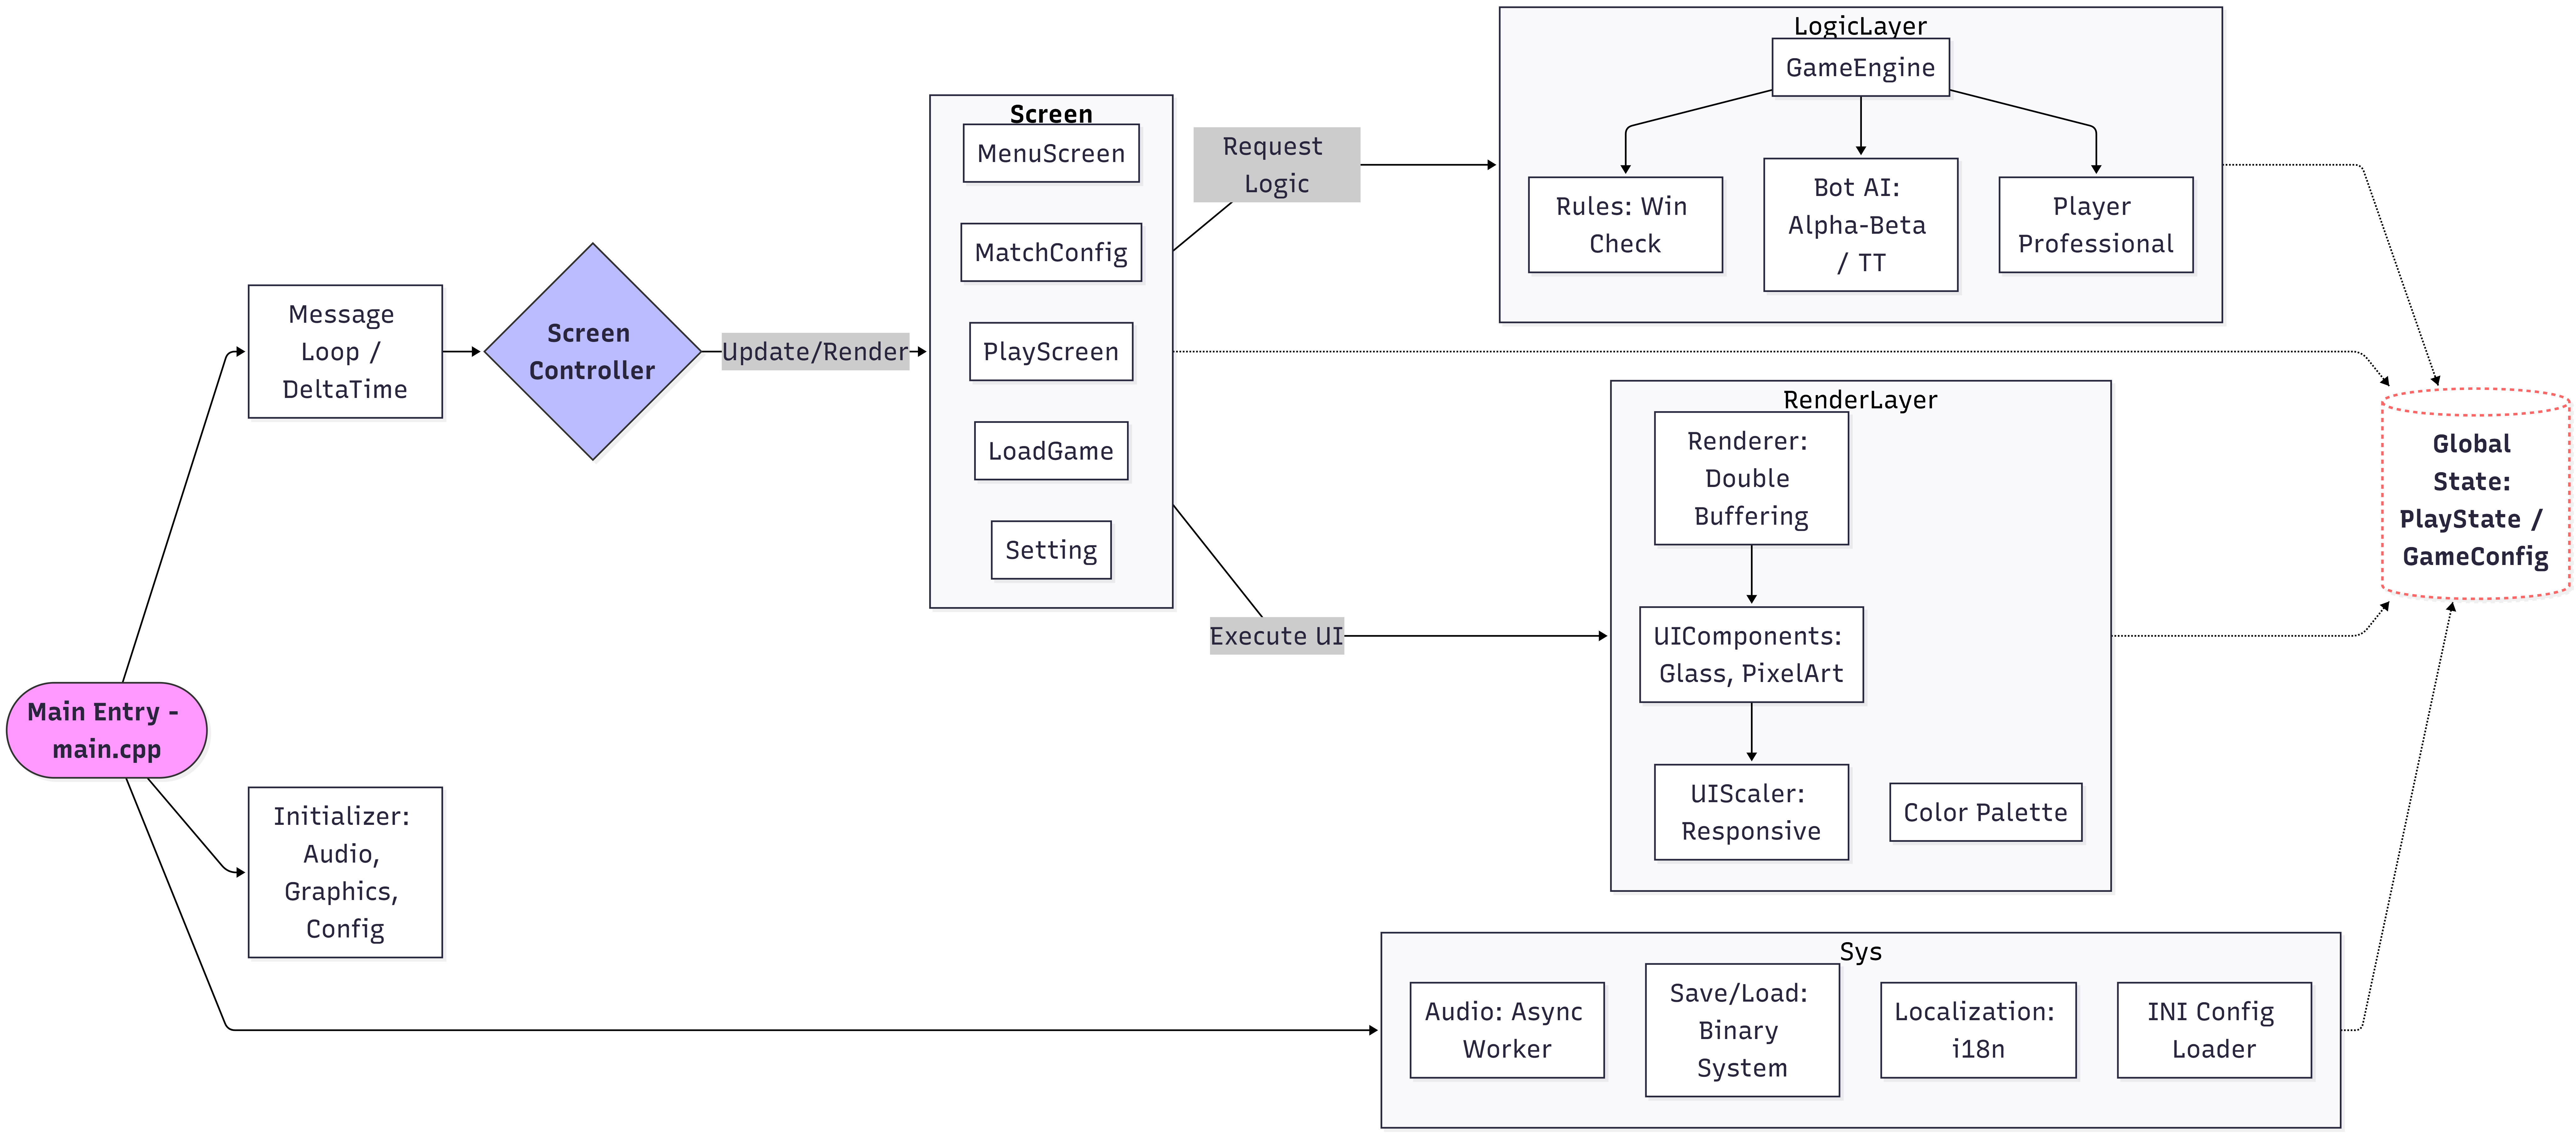
\includegraphics[width=1.4\linewidth, angle=90]{images/uml.png}
    \caption*{Hình 2.1: Sơ đồ kiến trúc hệ thống}
    \addcontentsline{lof}{figure}{Hình 2.1: Sơ đồ kiến trúc hệ thống}
\end{figure}

\textbf{Diễn giải chi tiết các mối quan hệ:}
\begin{itemize}
    \item \textbf{Luồng khởi tạo và vòng lặp chính:} Từ \texttt{main.cpp}, khối khởi tạo nạp Audio/Graphics/Config, sau đó đi vào \textit{Message Loop/DeltaTime}. Nhịp cập nhật này là nguồn kích hoạt cho \textit{Screen Controller}.
    \item \textbf{Tầng điều phối (Screen Controller):} Bộ điều phối chọn màn hình hiện tại (\texttt{MenuScreen}, \texttt{MatchConfig}, \texttt{PlayScreen}, \texttt{LoadGame}, \texttt{Setting}) và gọi \textit{Update/Render}. Khi cần xử lý nước đi hoặc luật, nó gửi \textit{Request Logic} sang \\ \texttt{GameEngine}.
    \item \textbf{LogicLayer:} \texttt{GameEngine} điều phối luật và lượt chơi, gọi \texttt{GameRules} để kiểm tra thắng, dùng \texttt{BotAI} (Alpha-Beta/TT) cho PvE và \texttt{PlayerEngineer} để xử lý thao tác người chơi. Tầng này chỉ làm việc với dữ liệu bàn cờ/trạng thái.
    \item \textbf{RenderLayer:} \texttt{Renderer} dựng khung hình bằng double buffering, \texttt{UIComponents} vẽ Glass/PixelArt, \texttt{UIScaler} đảm bảo responsive, và \texttt{Colours} cung cấp bảng màu đồng nhất.
    \item \textbf{Sys:} Các dịch vụ nền gồm Audio Async Worker, Save/Load Binary, Localization (i18n) và INI Config Loader, được các màn hình và logic gọi theo nhu cầu.
    \item \textbf{Global State:} \texttt{PlayState} và \texttt{GameConfig} là nguồn dữ liệu trung tâm. Logic cập nhật, Render đọc để vẽ, còn Sys đọc/ghi khi lưu/tải hoặc nạp cấu hình, bảo đảm tính nhất quán giữa các tầng.
\end{itemize}


\subsection*{2.2.4. Sơ đồ luồng chương trình}
\addcontentsline{toc}{subsection}{\textcolor{black}{2.2.4. Sơ đồ luồng chương trình}}

\noindent \indent Sơ đồ luồng dưới đây mô tả quá trình từ khi khởi chạy ứng dụng, điều hướng qua các màn hình chức năng cho đến khi kết thúc một vòng đời của trận đấu và thoát chương trình:

\begin{figure}[H]
    \centering
    \includegraphics[width=0.9\linewidth]{images/uml2.png}
    \caption*{Hình 2.2: Sơ đồ luồng chương trình}
    \addcontentsline{lof}{figure}{Hình 2.2: Sơ đồ luồng chương trình}
\end{figure}

\textbf{Mô tả các nút thắt quyết định:}

\begin{itemize}
    \item \textbf{Khởi tạo hệ thống:} Bắt đầu \textrightarrow{} khởi tạo GDI+, Audio, Config. Sau khi sẵn sàng, chương trình chuyển vào luồng điều hướng chính.
    \item \textbf{Điều hướng từ Màn hình chính:} 
    \begin{itemize}
        \item \textit{Chơi} \textrightarrow{} Thiết lập trận đấu \textrightarrow{} Màn hình Play (bắt đầu trận).
        \item \textit{Tải trận} \textrightarrow{} Danh sách bản lưu \textrightarrow{} Chọn slot \textrightarrow{} Xác nhận \textrightarrow{} Màn hình Play.
        \item \textit{Cài đặt} \textrightarrow{} Tùy chỉnh âm thanh/ngôn ngữ.
        \item \textit{Hướng dẫn/Thông tin} \textrightarrow{} Xem tài liệu/giới thiệu.
        \item \textit{Thoát} \textrightarrow{} Giải phóng tài nguyên và kết thúc.
    \end{itemize}
    \item \textbf{Vòng lặp trận đấu (Match Loop):} Màn hình Play nhận input di chuyển/đặt quân \textrightarrow{} logic xử lý (đánh quân hoặc AI tính toán) \textrightarrow{} kiểm tra thắng/hòa. Nếu \textit{chưa} kết thúc, quay lại vòng lặp; nếu \textit{kết thúc ván}, chuyển sang Bảng tổng kết.
    \item \textbf{Menu tạm và Lưu:} Trong khi chơi, nhấn \textit{ESC} mở Menu tạm, cho phép tiếp tục, lưu, hoặc thoát về màn hình chính. Lưu sẽ ghi \texttt{PlayState} ra file để có thể tải lại ở lần sau.
    \item \textbf{Tổng kết và điều hướng sau ván:} Bảng tổng kết ván đấu cho phép lưu, chơi ván tiếp theo (quay lại Match Loop), hoặc trở về Màn hình chính/thoát.
\end{itemize}

\section*{2.3. Cấu trúc thư mục và phân hệ}
\addcontentsline{toc}{section}{\textcolor{black}{2.3. Cấu trúc thư mục và phân hệ}}

\noindent \indent Dự án được tổ chức theo cấu trúc phân rã chức năng nghiêm ngặt, giúp việc quản lý hàng chục tệp tin mã nguồn trở nên khoa học và tránh hiện tượng chồng chéo định nghĩa.

\noindent \indent Cấu trúc thư mục tổng quát của mã nguồn được thể hiện như sau:

{\small
\begin{verbatim}
src/
|---- ApplicationTypes/
|     |---- GameConfig.h
|     |---- GameConstants.h
|     |---- GameState.h
|     |---- PlayState.h
|---- GameLogic/
|     |---- BotAI.cpp
|     |---- BotAI.h
|     |---- GameEngine.cpp
|     |---- GameEngine.h
|     |---- GameRules.cpp
|     |---- GameRules.h
|     |---- PlayerEngineer.cpp
|     |---- PlayerEngineer.h
|---- RenderAPI/
|     |---- Colours.cpp
|     |---- Colours.h
|     |---- Renderer.cpp
|     |---- Renderer.h
|     |---- UIComponents.cpp
|     |---- UIComponents.h
|     |---- UIScaler.cpp
|     |---- UIScaler.h
|---- ScreenModules/
|     |---- AboutScreen.cpp
|     |---- AboutScreen.h
|     |---- GuildScreen.cpp
|     |---- GuildScreen.h
|     |---- LoadGameScreen.cpp
|     |---- LoadGameScreen.h
|     |---- MatchConfigScreen.cpp
|     |---- MatchConfigScreen.h
|     |---- MenuScreen.cpp
|     |---- MenuScreen.h
|     |---- PlayScreen.cpp
|     |---- PlayScreen.h
|     |---- SettingScreen.cpp
|     |---- SettingScreen.h
|---- SystemModules/
|     |---- AudioSystem.cpp
|     |---- AudioSystem.h
|     |---- ConfigLoader.cpp
|     |---- ConfigLoader.h
|     |---- Localization.cpp
|     |---- Localization.h
|     |---- SaveLoadSystem.cpp
|     |---- SaveLoadSystem.h
|     |---- TimeSystem.cpp
|     |---- TimeSystem.h
|---- Asset/
|     |---- config.ini
|     |---- audio/
|     |---- font/
|     |---- lang/
|     |---- models/
|     |---- save/
|---- main.cpp
|---- src.sln
|---- src.vcxproj
|---- src.vcxproj.filters
\end{verbatim}
}

\subsection*{2.3.1. Chi tiết các phân hệ: RenderAPI, GameLogic, ScreenModules và SystemModules}
\addcontentsline{toc}{subsection}{\textcolor{black}{2.3.1. Chi tiết các phân hệ}}

\noindent \indent Mã nguồn và tài nguyên được chia thành 6 thư mục cốt lõi, mỗi thư mục đảm nhiệm một vai trò chuyên biệt trong vòng đời của ứng dụng. Dưới đây là mô tả đầy đủ theo từng phân hệ, nêu rõ trách nhiệm, phạm vi dữ liệu và các mô-đun chính:

\begin{itemize}
    \item \textbf{Phân hệ ApplicationTypes (Nền tảng dữ liệu):}
    Đây là nơi định nghĩa các kiểu dữ liệu và hằng số dùng chung cho toàn bộ dự án, làm "hợp đồng dữ liệu" giữa các tầng. Các tệp tiêu biểu gồm:
    \begin{itemize}
        \item \texttt{GameConfig.h}: lưu cấu hình trận đấu (chế độ chơi, kích thước bàn cờ, thời gian, âm lượng) để các phân hệ khác đọc thống nhất.
        \item \texttt{GameConstants.h}: tập hợp các hằng số hệ thống (kích thước ô, giới hạn mảng, mã trạng thái) nhằm tránh rải rác magic number.
        \item \texttt{GameState.h}: định nghĩa trạng thái tổng quát của ứng dụng và trận đấu (ví dụ: đang ở menu, đang chơi, đang tổng kết).
        \item \texttt{PlayState.h}: cấu trúc trung tâm lưu trạng thái bàn cờ, lượt chơi, lịch sử nước đi, thông số người chơi/AI.
    \end{itemize}
    Việc tập trung dữ liệu tại đây giúp đảm bảo tính nhất quán khi các phân hệ khác cùng truy cập và cập nhật.

    \item \textbf{Phân hệ RenderAPI (Thư viện đồ họa nội bộ):}
    Đóng vai trò là lớp vỏ bọc cho GDI+, cung cấp các công cụ vẽ bậc cao và nhất quán giao diện:
    \begin{itemize}
        \item \texttt{Colours}: quản lý bảng màu, đảm bảo toàn bộ giao diện dùng cùng hệ màu (nút, nền, hiệu ứng).
        \item \texttt{Renderer}: khởi tạo ngữ cảnh đồ họa, quản lý back buffer và thực hiện quy trình vẽ khung hình.
        \item \texttt{UIComponents}: dựng các thành phần giao diện (bàn cờ, quân cờ, nút) từ dữ liệu mô tả.
        \item \texttt{UIScaler}: tính toán tỷ lệ và chuyển đổi tọa độ nhằm hỗ trợ đa độ phân giải và tỷ lệ màn hình.
    \end{itemize}
    Tầng này chỉ nhận dữ liệu đã được chuẩn hóa và không tự ý thay đổi logic trận đấu.

    \item \textbf{Phân hệ GameLogic (Đầu não xử lý):}
    Tập trung vào quy tắc, điều phối trận đấu và trí tuệ nhân tạo:
    \begin{itemize}
        \item \texttt{GameEngine}: điều phối vòng đời trận đấu, xử lý đặt quân, chuyển lượt, kiểm soát trạng thái và lịch sử nước đi.
        \item \texttt{GameRules}: kiểm tra điều kiện thắng, hòa, hợp lệ nước đi theo hàng ngang, dọc, chéo.
        \item \texttt{BotAI}: tính toán nước đi tối ưu cho chế độ PvE, tách biệt khỏi phần đồ họa.
        \item \texttt{PlayerEngineer}: xử lý thao tác người chơi và chuyển dữ liệu đầu vào thành nước đi trước khi chuyển sang \texttt{GameEngine}.
    \end{itemize}
    Mọi xử lý trong phân hệ này chỉ làm việc với dữ liệu thuần (ma trận bàn cờ, trạng thái), không phụ thuộc GDI+.

    \item \textbf{Phân hệ ScreenModules (Quản lý màn hình):}
    Mỗi tệp trong thư mục này tương ứng một màn hình cụ thể, chịu trách nhiệm xử lý input, điều hướng và cập nhật trạng thái hiển thị:
    \begin{itemize}
        \item \texttt{MenuScreen}: màn hình chính, điều hướng đến các chế độ chơi và thiết lập.
        \item \texttt{PlayScreen}: màn hình trận đấu, kết nối trực tiếp với \texttt{GameEngine} và \texttt{Renderer}.
        \item \texttt{MatchConfigScreen}: cấu hình trận đấu (chế độ, nhân vật, luật chơi).
        \item \texttt{LoadGameScreen}: tải trận đã lưu, khôi phục \texttt{PlayState}.
        \item \texttt{SettingScreen}: điều chỉnh âm lượng, ngôn ngữ, tùy chọn hiển thị.
        \item \texttt{AboutScreen} và \texttt{GuildScreen}: các màn hình thông tin/bảng thành tích.
    \end{itemize}
    Cách tổ chức này giúp mỗi màn hình có vòng đời rõ ràng, tránh chồng chéo xử lý.

    \item \textbf{Phân hệ SystemModules (Dịch vụ nền):}
    Cung cấp các dịch vụ hỗ trợ cho toàn ứng dụng:
    \begin{itemize}
        \item \texttt{AudioSystem}: quản lý âm thanh đa luồng, phát nhạc nền và hiệu ứng.
        \item \texttt{ConfigLoader}: tải và lưu cấu hình người dùng từ \texttt{config.ini}.
        \item \texttt{Localization}: nạp và ánh xạ chuỗi đa ngôn ngữ từ tệp tài nguyên.
        \item \texttt{SaveLoadSystem}: lưu/khôi phục \texttt{PlayState} xuống ổ đĩa.
        \item \texttt{TimeSystem}: cung cấp bộ đếm thời gian và đo độ trễ khung hình.
    \end{itemize}
    Các dịch vụ này độc lập với logic trận đấu và được gọi theo nhu cầu của các màn hình.

    \item \textbf{Phân hệ Asset (Tài nguyên dữ liệu):}
    Lưu trữ toàn bộ tài nguyên đầu vào của trò chơi, tách biệt khỏi mã nguồn để dễ cập nhật:
    \begin{itemize}
        \item \texttt{config.ini}: cấu hình người dùng và thiết lập mặc định.
        \item \texttt{audio/}: tệp nhạc nền và hiệu ứng âm thanh.
        \item \texttt{font/}: phông chữ hiển thị trong giao diện.
        \item \texttt{lang/}: tệp ngôn ngữ (Việt/Anh) dùng cho \texttt{Localization}.
        \item \texttt{models/}: dữ liệu pixel art, hình nền, vật thể.
        \item \texttt{save/}: dữ liệu lưu trận và lịch sử chơi.
    \end{itemize}
    Thư mục này giúp tách biệt nội dung và logic, cho phép thay đổi tài nguyên mà không cần biên dịch lại.
\end{itemize}

\subsection*{2.3.2. Quy ước Header, Cấu trúc dữ liệu và Đóng gói dữ liệu}
\addcontentsline{toc}{subsection}{\textcolor{black}{2.3.2. Quy ước Header, Cấu trúc dữ liệu và Đóng gói dữ liệu}}

\noindent \indent Để duy trì tính ổn định của mã nguồn, dự án áp dụng các quy chuẩn lập trình đồng bộ, đảm bảo khả năng mở rộng và giảm lỗi phát sinh khi nhiều mô-đun cùng phát triển:

\begin{itemize}
    \item \textbf{Quy ước tệp tiêu đề (Header Guards):}
    Tất cả các tệp \texttt{.h} đều dùng \texttt{\#ifndef / \#define / \#endif} để chống khai báo trùng lặp. Tên guard được đặt theo tên file và phân hệ để tránh va chạm (ví dụ: \texttt{GAMELOGIC\_GAMEENGINE\_H}).

    \item \textbf{Tổ chức Cấu trúc và Kiểu liệt kê (Struct/Enum):}
    \begin{itemize}
        \item Enum được dùng để mô tả trạng thái màn hình, chế độ chơi và trạng thái trận đấu, giúp logic điều phối rõ ràng và tránh dùng số "ẩn".
        \item Struct được thiết kế theo hướng dữ liệu thuần (POD), bao gồm các trường cần thiết cho hiển thị và xử lý (bàn cờ, lượt chơi, điểm, thời gian), không nhúng thuật toán bên trong.
        \item Các struct trong \texttt{ApplicationTypes} là nguồn dữ liệu chuẩn cho cả \texttt{GameLogic} và \texttt{RenderAPI}, tránh trùng lặp định nghĩa.
    \end{itemize}

    \item \textbf{Cơ chế đóng gói và Quản lý biến toàn cục:}
    \begin{itemize}
        \item Các biến trạng thái dùng chung (như cấu hình và trạng thái trận) được khai báo \texttt{extern} trong header và định nghĩa duy nhất tại tệp triển khai để mọi mô-đun truy cập đồng nhất.
        \item Biến nội bộ của từng màn hình được giới hạn phạm vi bằng \texttt{static} trong file \texttt{.cpp} để tránh va chạm tên và giảm rủi ro chỉnh sửa ngoài ý muốn.
        \item Mọi thay đổi lên dữ liệu dùng chung đều đi qua các hàm điều phối (ví dụ: từ \texttt{GameEngine} hoặc \texttt{ScreenModules}) để đảm bảo thứ tự cập nhật nhất quán.
    \end{itemize}

    \item \textbf{Tách biệt giao diện và thực thi:}
    Các tệp \texttt{.h} chỉ khai báo lớp/hàm cần thiết, còn phần triển khai đặt trong \texttt{.cpp}. Điều này giúp giảm phụ thuộc chéo, rút ngắn thời gian biên dịch và tạo giao diện lập trình rõ ràng giữa các phân hệ.

    \item \textbf{Quy ước lưu trữ và tuần tự hóa dữ liệu:}
    Dữ liệu trận đấu được lưu dưới dạng nhị phân thông qua \texttt{SaveLoadSystem}, đảm bảo tốc độ đọc/ghi cao và khôi phục đúng trạng thái. Cấu hình người dùng được lưu trong \texttt{config.ini} để dễ chỉnh sửa và tương thích lâu dài.
\end{itemize}

\newpage
\chapter*{\centering CHƯƠNG 3. THIẾT KẾ DỮ LIỆU VÀ CẤU TRÚC CỐT LÕI}
\addcontentsline{toc}{chapter}{\textcolor{fitblue}{CHƯƠNG 3. THIẾT KẾ DỮ LIỆU VÀ CẤU TRÚC CỐT LÕI}}

\section*{3.1. Quản lý trạng thái ván đấu}
\addcontentsline{toc}{section}{\textcolor{black}{3.1. Quản lý trạng thái ván đấu}}

\noindent \indent Lõi dữ liệu của toàn bộ hệ thống được gom vào cấu trúc \texttt{PlayState}. Cấu trúc này lưu tất cả thông tin cần thiết để khôi phục ván đấu, điều phối lượt đi, hiển thị giao diện và hỗ trợ lưu/tải. Dữ liệu được thiết kế theo hướng POD để tối ưu hiệu năng và đơn giản hóa việc tuần tự hóa.

\subsection*{3.1.1. Ma trận bàn cờ và tối ưu bộ nhớ}
\addcontentsline{toc}{subsection}{\textcolor{black}{3.1.1. Ma trận bàn cờ và tối ưu bộ nhớ}}

\noindent \indent Bàn cờ được lưu dưới dạng mảng tĩnh hai chiều, kết hợp các hằng số hệ thống trong \texttt{GameConstants.h}. Thiết kế này tránh cấp phát động lặp lại, giúp truy cập theo chỉ số O(1) và giảm overhead khi kiểm tra luật thắng.

\begin{itemize}
  \item \textbf{Kích thước và giới hạn:} \texttt{GOMOKU\_SIZE = 15}, \texttt{WIN\_CONDITION = 5}, \\ \texttt{MAX\_BOARD\_SIZE = 20} đảm bảo đủ vùng đệm cho mọi chế độ.
  \item \textbf{Giá trị ô:} mỗi ô mang một trong ba trạng thái \texttt{CELL\_EMPTY}, \texttt{CELL\_PLAYER1}, \texttt{CELL\_PLAYER2}.
  \item \textbf{Kích thước thực tế:} \texttt{boardSize} cho phép chuyển giữa Caro (15x15) và TTT (3x3) mà không đổi cấu trúc lưu trữ.
\end{itemize}

\begin{table}[H]
\captionsetup{type=lstlisting}
\caption{Mã nguồn Hằng số và định nghĩa trạng thái ô bàn cờ}
\label{lst:gameconstants}
\centering
\renewcommand{\arraystretch}{0.8}
\begin{tabularx}{\linewidth}{|>{\ttfamily\small\color{black}\raggedleft\arraybackslash}p{0.8cm}|>{\ttfamily\small\color{black}\arraybackslash}X|}
\hline
\normalfont\bfseries STT & \normalfont\bfseries Mã nguồn \\ \hline
1 & \cppkw{\#define} GOMOKU\_SIZE 15 \\ \hline
2 & \cppkw{\#define} WIN\_CONDITION 5 \\ \hline
3 & \cppkw{\#define} MAX\_BOARD\_SIZE 20 \\ \hline
4 &  \\ \hline
5 & \cppkw{\#define} CELL\_EMPTY 0 \\ \hline
6 & \cppkw{\#define} CELL\_PLAYER1 1 \\ \hline
7 & \cppkw{\#define} CELL\_PLAYER2 2 \\ \hline
8 &  \\ \hline
9 & \cppkw{\#define} MAX\_SAVE\_SLOTS 5 \textcolor{dkgreen}{// Giới hạn 5 slot lưu game} \\ \hline
10 & \cppkw{\#define} MAX\_SAVE\_NAME\_LEN 15 \textcolor{dkgreen}{// Giới hạn 15 ký tự cho tên/thông tin hiển thị} \\ \hline
\end{tabularx}
\end{table}

\begin{table}[H]
\captionsetup{type=lstlisting}
\caption{Mã nguồn Ma trận bàn cờ trong PlayState}
\label{lst:playstate_board}
\centering
\renewcommand{\arraystretch}{0.8}
\begin{tabularx}{\linewidth}{|>{\ttfamily\small\color{black}\raggedleft\arraybackslash}p{0.8cm}|>{\ttfamily\small\color{black}\arraybackslash}X|}
\hline
\normalfont\bfseries STT & \normalfont\bfseries Mã nguồn \\ \hline
1 & \cppkw{int} boardSize = 15; \\ \hline
2 & \textcolor{dkgreen}{// Ma trận lưu giá trị: CELL\_EMPTY, CELL\_PLAYER1, hoặc CELL\_PLAYER2} \\ \hline
3 & \cppkw{int} board[MAX\_BOARD\_SIZE][MAX\_BOARD\_SIZE] = {0}; \\ \hline
\end{tabularx}
\end{table}

\subsection*{3.1.2. Turn-based logic và Match Status}
\addcontentsline{toc}{subsection}{\textcolor{black}{3.1.2. Turn-based logic và Match Status}}

\noindent \indent Vòng đời ván đấu được điều phối bằng các trường trạng thái trong \texttt{PlayState} và enum \texttt{MatchStatus}. Trạng thái này là cơ sở để GameEngine quyết định xử lý nước đi, tạm dừng hoặc tổng kết.

\begin{itemize}
  \item \textbf{Lượt chơi:} \texttt{isP1Turn} quyết định quân cờ đang được đặt và cập nhật đếm lượt.
  \item \textbf{Trạng thái ván:} \texttt{MATCH\_PLAYING}, \texttt{MATCH\_PAUSED}, \texttt{MATCH\_FINISHED}, \\ \texttt{MATCH\_SUMMARY}.
  \item \textbf{Kết quả:} \texttt{winner} lưu giá trị \texttt{-1} (đang chơi), \texttt{0} (hòa), \texttt{1} (P1), \texttt{2} (P2).
  \item \textbf{Thời gian:} \texttt{countdownTime} và \texttt{timeRemaining} quản lý thời gian lượt; \\ \texttt{isMatchTimed}, \texttt{p1TotalTimeLeft}, \texttt{p2TotalTimeLeft} quản lý thời gian toàn trận.
\end{itemize}

\begin{table}[H]
\captionsetup{type=lstlisting}
\caption{Mã nguồn Enum MatchStatus trong PlayState}
\label{lst:matchstatus}
\centering
\renewcommand{\arraystretch}{0.8}
\begin{tabularx}{\linewidth}{|>{\ttfamily\small\color{black}\raggedleft\arraybackslash}p{0.8cm}|>{\ttfamily\small\color{black}\arraybackslash}X|}
\hline
\normalfont\bfseries STT & \normalfont\bfseries Mã nguồn \\ \hline
1 & \cppkw{enum} MatchStatus \\ \hline
2 & \{ \\ \hline
3 & \ \ MATCH\_PLAYING, \\ \hline
4 & \ \ MATCH\_PAUSED, \\ \hline
5 & \ \ MATCH\_FINISHED, \\ \hline
6 & \ \ MATCH\_SUMMARY \\ \hline
7 & \}; \\ \hline
\end{tabularx}
\end{table}

\subsection*{3.1.3. Lịch sử nước đi và cơ chế Undo/Redo}
\addcontentsline{toc}{subsection}{\textcolor{black}{3.1.3. Lịch sử nước đi và cơ chế Undo/Redo}}

\noindent \indent Dữ liệu lịch sử được lưu trong \texttt{matchHistory} và \texttt{redoStack}. Điều này cho phép hoàn tác và thực hiện lại một cách nhất quán giữa PvP và PvE.

\begin{itemize}
  \item \textbf{matchHistory:} chuỗi các tọa độ đã đánh, dùng để khôi phục và tính toán kết quả.
  \item \textbf{redoStack:} lưu các nước đã hoàn tác để có thể thực hiện lại.
  \item \textbf{lastMoveRow/Col và winningCells:} phục vụ hiển thị nước đi cuối và highlight chuỗi thắng.
\end{itemize}

\begin{table}[H]
\captionsetup{type=lstlisting}
\caption{Mã nguồn Quy tắc Undo cho PvE (lùi 2 nước)}
\label{lst:undo_pve}
\centering
\renewcommand{\arraystretch}{0.8}
\begin{tabularx}{\linewidth}{|>{\ttfamily\small\color{black}\raggedleft\arraybackslash}p{0.8cm}|>{\ttfamily\small\color{black}\arraybackslash}X|}
\hline
\normalfont\bfseries STT & \normalfont\bfseries Mã nguồn \\ \hline
1 & \cppkw{void} undoMove(PlayState* state) \{ \\ \hline
2 & \ \ \cppkw{if} (state->matchHistory.empty()) \cppkw{return}; \\ \hline
3 &  \\ \hline
4 & \ \ \textcolor{dkgreen}{// PVE: lùi 2 bước để trả lượt về người chơi} \\ \hline
5 & \ \ \cppkw{int} popCount = (state->matchType == MATCH\_PVE \\ \hline
6 & \ \ \ \ \&\& state->matchHistory.size() >= 2) ? 2 : 1; \\ \hline
\end{tabularx}
\end{table}

\subsection*{3.1.4. Kiểm tra điều kiện thắng và trạng thái kết thúc}
\addcontentsline{toc}{subsection}{\textcolor{black}{3.1.4. Kiểm tra điều kiện thắng và trạng thái kết thúc}}

\noindent \indent Luật thắng được xử lý trong \texttt{GameRules::checkWinCondition}. Hệ thống tự động chọn độ dài thắng theo chế độ (Caro: 5, TTT: 3), quét 4 hướng và trả về toàn bộ chuỗi thắng để hiển thị.

\begin{table}[H]
\captionsetup{type=lstlisting}
\caption{Mã nguồn Xác định độ dài thắng theo chế độ chơi}
\label{lst:winlen}
\centering
\renewcommand{\arraystretch}{0.8}
\begin{tabularx}{\linewidth}{|>{\ttfamily\small\color{black}\raggedleft\arraybackslash}p{0.8cm}|>{\ttfamily\small\color{black}\arraybackslash}X|}
\hline
\normalfont\bfseries STT & \normalfont\bfseries Mã nguồn \\ \hline
1 & \cppkw{const} \cppkw{int} winLength = (state->gameMode == MODE\_CARO) ? 5 : 3; \\ \hline
2 & \cppkw{const} \cppkw{int} size = state->boardSize; \\ \hline
\end{tabularx}
\end{table}

\begin{table}[H]
\captionsetup{type=lstlisting}
\caption{Mã nguồn Trả về toàn bộ chuỗi thắng để highlight}
\label{lst:winline}
\centering
\renewcommand{\arraystretch}{0.8}
\begin{tabularx}{\linewidth}{|>{\ttfamily\small\color{black}\raggedleft\arraybackslash}p{0.8cm}|>{\ttfamily\small\color{black}\arraybackslash}X|}
\hline
\normalfont\bfseries STT & \normalfont\bfseries Mã nguồn \\ \hline
1 & \cppkw{if} ((\cppkw{int})line.size() >= winLength) \{ \\ \hline
2 & \ \ \cppkw{if} (outWinCells) \\ \hline
3 & \ \ \ \ *outWinCells = line; \textcolor{dkgreen}{// Trả về toàn bộ chuỗi, không cắt} \\ \hline
4 & \ \ \cppkw{return} currentPiece; \\ \hline
5 & \} \\ \hline
\end{tabularx}
\end{table}

\section*{3.2. Mô hình người chơi}
\addcontentsline{toc}{section}{\textcolor{black}{3.2. Mô hình người chơi}}

\noindent \indent Thông tin người chơi được chuẩn hóa qua \texttt{PlayerInfo2}. Cấu trúc này tập trung các thống kê phục vụ hiển thị, tính điểm và lưu/tải.

\subsection*{3.2.1. PlayerInfo2: Wins, Moves, Possession Time}
\addcontentsline{toc}{subsection}{\textcolor{black}{3.2.1. PlayerInfo2: Wins, Moves, Possession Time}}

\begin{itemize}
  \item \textbf{name, avatarPath, piece:} thông tin định danh và quân cờ đại diện.
  \item \textbf{totalWins:} số ván thắng trong series BO hiện tại.
  \item \textbf{matchWins:} số series BO đã thắng.
  \item \textbf{movesCount:} tổng số nước đã đi trong ván.
  \item \textbf{maxTurnTime, totalTimePossessed:} giới hạn thời gian lượt và tổng thời gian giữ lượt.
\end{itemize}

\begin{table}[H]
\captionsetup{type=lstlisting}
\caption{Mã nguồn Cấu trúc PlayerInfo2}
\label{lst:playerinfo2}
\centering
\renewcommand{\arraystretch}{0.8}
\begin{tabularx}{\linewidth}{|>{\ttfamily\small\color{black}\raggedleft\arraybackslash}p{0.8cm}|>{\ttfamily\small\color{black}\arraybackslash}X|}
\hline
\normalfont\bfseries STT & \normalfont\bfseries Mã nguồn \\ \hline
1 & \cppkw{struct} PlayerInfo2 \\ \hline
2 & \{ \\ \hline
3 & \ \ \cppkw{wstring} name; \\ \hline
4 & \ \ \cppkw{string} avatarPath; \\ \hline
5 & \ \ \cppkw{char} piece = ' '; \textcolor{dkgreen}{// 'X' hoặc 'O'} \\ \hline
6 & \ \ \cppkw{int} totalWins = 0; \textcolor{dkgreen}{// Số Bàn Thắng (trong series BO hiện tại)} \\ \hline
7 & \ \ \cppkw{int} matchWins = 0; \textcolor{dkgreen}{// Số Trận Thắng BO (đã thắng trọn 1 serie BO)} \\ \hline
8 & \ \ \cppkw{int} movesCount = 0; \\ \hline
9 & \ \ \cppkw{float} maxTurnTime = 0.0f; \textcolor{dkgreen}{// Thời gian tối đa cho 1 lượt} \\ \hline
10 & \ \ \cppkw{float} totalTimePossessed = 0.0f; \textcolor{dkgreen}{// Tổng thời gian giữ bóng (giây), cộng dồn theo phiên} \\ \hline
11 & \}; \\ \hline
\end{tabularx}
\end{table}

\subsection*{3.2.2. PlayerEngineer và vòng đời thực thể}
\addcontentsline{toc}{subsection}{\textcolor{black}{3.2.2. PlayerEngineer và vòng đời thực thể}}

\noindent \indent \texttt{PlayerEngineer} đóng vai trò khởi tạo và reset chỉ số theo vòng đời ván đấu. Các thao tác này được GameEngine gọi khi bắt đầu match hoặc round mới.

\begin{itemize}
  \item \textbf{initPlayer:} gán tên, avatar, quân cờ và reset các thống kê cần thiết.
  \item \textbf{resetPlayerForRound:} chỉ reset thống kê theo round (ví dụ \texttt{movesCount}), giữ nguyên tiến trình series BO.
\end{itemize}

\begin{table}[H]
\captionsetup{type=lstlisting}
\caption{Mã nguồn Reset thống kê theo round trong PlayerEngineer}
\label{lst:resetplayer}
\centering
\renewcommand{\arraystretch}{0.8}
\begin{tabularx}{\linewidth}{|>{\ttfamily\small\color{black}\raggedleft\arraybackslash}p{0.8cm}|>{\ttfamily\small\color{black}\arraybackslash}X|}
\hline
\normalfont\bfseries STT & \normalfont\bfseries Mã nguồn \\ \hline
1 & \cppkw{void} resetPlayerForRound(PlayerInfo2\& player) \{ \\ \hline
2 & \ \ player.movesCount = 0; \\ \hline
3 & \ \ \textcolor{dkgreen}{// Lưu ý: totalWins và matchWins được giữ nguyên để tính tiến trình series BO} \\ \hline
4 & \} \\ \hline
\end{tabularx}
\end{table}

\section*{3.3. Cấu hình và môi trường}
\addcontentsline{toc}{section}{\textcolor{black}{3.3. Cấu hình và môi trường}}

\subsection*{3.3.1. Nạp Config và thiết lập mặc định}
\addcontentsline{toc}{subsection}{\textcolor{black}{3.3.1. Nạp Config và thiết lập mặc định}}

\noindent \indent Thông số hệ thống (âm thanh, ngôn ngữ) được gói trong \texttt{GameConfig}. \texttt{ConfigLoader} đọc/ghi trực tiếp cấu trúc này theo dạng nhị phân và tự tạo mặc định nếu thiếu tệp.

\begin{itemize}
  \item \textbf{Audio:} \texttt{isBgmEnabled}, \texttt{bgmVolume}, \texttt{isSfxEnabled}, \texttt{sfxVolume}.
  \item \textbf{Language:} \texttt{currentLang} với hai lựa chọn \texttt{APP\_LANG\_VI} và \texttt{APP\_LANG\_EN}.
\end{itemize}

\begin{table}[H]
\captionsetup{type=lstlisting}
\caption{Mã nguồn Thiết lập mặc định trong ConfigLoader}
\label{lst:defaultconfig}
\centering
\renewcommand{\arraystretch}{0.8}
\begin{tabularx}{\linewidth}{|>{\ttfamily\small\color{black}\raggedleft\arraybackslash}p{0.8cm}|>{\ttfamily\small\color{black}\arraybackslash}X|}
\hline
\normalfont\bfseries STT & \normalfont\bfseries Mã nguồn \\ \hline
1 & \cppkw{static} \cppkw{void} SetDefaultConfig(GameConfig* config) \{ \\ \hline
2 & \ \ config->isBgmEnabled = \cppkw{true}; \\ \hline
3 & \ \ config->bgmVolume = 50; \\ \hline
4 & \ \ config->isSfxEnabled = \cppkw{true}; \\ \hline
5 & \ \ config->sfxVolume = 50; \\ \hline
6 & \ \ config->currentLang = APP\_LANG\_VI; \\ \hline
7 & \} \\ \hline
\end{tabularx}
\end{table}

\subsection*{3.3.2. Lưu/Tải trạng thái và metadata}
\addcontentsline{toc}{subsection}{\textcolor{black}{3.3.2. Lưu/Tải trạng thái và metadata}}

\noindent \indent Hệ thống lưu/tải được triển khai trong \texttt{SaveLoadSystem}. Mỗi bản lưu được quản lý theo slot, kèm metadata để hiển thị ở màn hình Load Game. File save có magic number và version để kiểm tra tính hợp lệ.

\begin{itemize}
  \item \textbf{MAX\_SAVE\_SLOTS = 5:} giới hạn số slot lưu.
  \item \textbf{SaveMetadata:} lưu tên, thời gian, chế độ, điểm và độ khó.
  \item \textbf{SAVE\_MAGIC / SAVE\_VERSION:} dùng để kiểm tra định dạng file và tương thích phiên bản.
\end{itemize}

\begin{table}[H]
\captionsetup{type=lstlisting}
\caption{Mã nguồn Cấu trúc metadata cho slot lưu}
\label{lst:savemetadata}
\centering
\renewcommand{\arraystretch}{0.8}
\begin{tabularx}{\linewidth}{|>{\ttfamily\small\color{black}\raggedleft\arraybackslash}p{0.8cm}|>{\ttfamily\small\color{black}\arraybackslash}X|}
\hline
\normalfont\bfseries STT & \normalfont\bfseries Mã nguồn \\ \hline
1 & \cppkw{struct} SaveMetadata \{ \\ \hline
2 & \ \ std::wstring name; \\ \hline
3 & \ \ std::wstring timestamp; \\ \hline
4 & \ \ \cppkw{int} mode; \textcolor{dkgreen}{// 0: Caro, 1: TTT} \\ \hline
5 & \ \ \cppkw{int} type; \textcolor{dkgreen}{// 0: PvP, 1: PvE} \\ \hline
6 & \ \ \cppkw{int} p1Wins; \\ \hline
7 & \ \ \cppkw{int} p2Wins; \\ \hline
8 & \ \ \cppkw{int} difficulty; \\ \hline
9 & \ \ \cppkw{int} boardSize; \\ \hline
10 & \ \ \cppkw{bool} exists; \\ \hline
11 & \ \ \cppkw{uint32\_t} version; \\ \hline
12 & \}; \\ \hline
\end{tabularx}
\end{table}

\begin{table}[H]
\captionsetup{type=lstlisting}
\caption{Mã nguồn Magic number và phiên bản file save}
\label{lst:savemagic}
\centering
\renewcommand{\arraystretch}{0.8}
\begin{tabularx}{\linewidth}{|>{\ttfamily\small\color{black}\raggedleft\arraybackslash}p{0.8cm}|>{\ttfamily\small\color{black}\arraybackslash}X|}
\hline
\normalfont\bfseries STT & \normalfont\bfseries Mã nguồn \\ \hline
1 & \cppkw{static} \cppkw{const} \cppkw{uint32\_t} SAVE\_MAGIC = 0xCA05A1E2; \\ \hline
2 & \cppkw{static} \cppkw{const} \cppkw{uint32\_t} SAVE\_VERSION = 5; \\ \hline
\end{tabularx}
\end{table}

\subsection*{3.3.3. Hệ thống màu sắc và theme động}
\addcontentsline{toc}{subsection}{\textcolor{black}{3.3.3. Hệ thống màu sắc và theme động}}

\noindent \indent Hệ thống màu được chuẩn hóa qua \texttt{SmartColor}, \texttt{Palette} và \texttt{Theme}. Điều này giúp giao diện đồng nhất, dễ mở rộng, và hỗ trợ pha trộn alpha cho hiệu ứng kính mờ và highlight.

\begin{itemize}
  \item \textbf{SmartColor:} cấu trúc ARGB dạng POD, dùng chung cho GDI và GDI+.
  \item \textbf{Palette:} tập hợp màu cơ bản (đen, trắng, xám, đỏ, xanh, cyan...) và các dải màu phụ trợ.
  \item \textbf{Theme:} màu theo ngữ nghĩa (panel, pitch, highlight, border, turn pulse).
\end{itemize}

\begin{table}[H]
\captionsetup{type=lstlisting}
\caption{Mã nguồn Cấu trúc SmartColor}
\label{lst:smartcolor}
\centering
\renewcommand{\arraystretch}{0.8}
\begin{tabularx}{\linewidth}{|>{\ttfamily\small\color{black}\raggedleft\arraybackslash}p{0.8cm}|>{\ttfamily\small\color{black}\arraybackslash}X|}
\hline
\normalfont\bfseries STT & \normalfont\bfseries Mã nguồn \\ \hline
1 & \cppkw{struct} SmartColor \\ \hline
2 & \{ \\ \hline
3 & \ \ \cppkw{BYTE} a; \\ \hline
4 & \ \ \cppkw{BYTE} r; \\ \hline
5 & \ \ \cppkw{BYTE} g; \\ \hline
6 & \ \ \cppkw{BYTE} b; \\ \hline
7 & \}; \\ \hline
\end{tabularx}
\end{table}

\captionsetup{type=lstlisting}
\renewcommand{\arraystretch}{0.8}

\captionof{lstlisting}{Mã nguồn Một số màu chủ đạo trong Theme}\label{lst:theme} 
\begin{longtable}{|>{\ttfamily\small\color{black}\raggedleft\arraybackslash}p{0.8cm}|>{\ttfamily\small\color{black}\arraybackslash}p{\dimexpr\linewidth-0.8cm-3\tabcolsep-2\arrayrulewidth}|}
\hline
\normalfont\bfseries STT & \normalfont\bfseries Mã nguồn \\ \hline
\endfirsthead

\hline
\normalfont\bfseries STT & \normalfont\bfseries Mã nguồn \\ \hline
\endhead

1 & \cppkw{constexpr} SmartColor GlassWhite = \{220, 255, 255, 255\}; \textcolor{dkgreen}{// Panel trắng mờ} \\ \hline
2 & \cppkw{constexpr} SmartColor GlassDark = \{200, 15, 20, 30\}; \textcolor{dkgreen}{// Panel tối (pause)} \\ \hline
3 & \cppkw{constexpr} SmartColor GlassGleam = \{150, 255, 255, 255\}; \textcolor{dkgreen}{// Viền trắng mờ} \\ \hline
4 &  \\ \hline
5 & \cppkw{constexpr} SmartColor P1TurnPulse = \{30, 255, 150, 0\}; \\ \hline
6 & \cppkw{constexpr} SmartColor P1TurnBorder = \{200, 255, 150, 0\}; \\ \hline
7 & \cppkw{constexpr} SmartColor P1Watermark = \{60, 255, 150, 0\}; \\ \hline
8 &  \\ \hline
9 & \cppkw{constexpr} SmartColor P2TurnPulse = \{30, 0, 255, 255\}; \\ \hline
10 & \cppkw{constexpr} SmartColor P2TurnBorder = \{200, 0, 255, 255\}; \\ \hline
11 & \cppkw{constexpr} SmartColor P2Watermark = \{60, 0, 255, 255\}; \\ \hline

\end{longtable}

\newpage
\chapter*{\centering CHƯƠNG 4. HỆ THỐNG ĐỒ HỌA VÀ UI/UX}
\addcontentsline{toc}{chapter}{\textcolor{fitblue}{CHƯƠNG 4. HỆ THỐNG ĐỒ HỌA VÀ UI/UX}}
\setlength{\parindent}{1.5em}

\section*{4.1. Tổng quan pipeline đồ họa}
\addcontentsline{toc}{section}{\textcolor{black}{4.1. Tổng quan pipeline đồ họa}}

\setlength{\parindent}{1.5em} Chương này trình bày toàn bộ kiến trúc đồ họa và UI/UX của trò chơi, dựa trên cấu trúc triển khai và các mô-đun hệ thống. Hệ thống được xây dựng trên Win32 API kết hợp GDI/GDI+ theo hướng ``raster + procedural'', nhấn mạnh tốc độ, độ mượt và cảm giác thị giác retro \cite{ms_windows_gdi}. Phần này không chỉ mô tả cách vẽ mà còn lý giải các tối ưu quan trọng (double buffering, cache bitmap, palette động) và cách các màn hình thực tế ghép các thành phần đó thành trải nghiệm người dùng nhất quán.

\setlength{\parindent}{1.5em} Về mặt kỹ thuật, vòng đời đồ họa bắt đầu từ \texttt{InitGraphics} (khởi động GDI+), kế tiếp là \\ \texttt{GlobalFont::Initialize} để nạp font VT323, sau đó tạo \texttt{DoubleBuffer} để vẽ toàn bộ frame lên HDC bộ nhớ. Khi thoát game, \texttt{GlobalFont::Cleanup} gỡ font đã nạp và \texttt{ShutdownGraphics} giải phóng token GDI+ nhằm tránh rò rỉ tài nguyên hệ thống.

\setlength{\parindent}{1.5em} Pipeline hiển thị chia làm hai lớp:
\begin{itemize}
  \item \textbf{Lớp khởi tạo và tài nguyên toàn cục}: GDI+ được khởi tạo, font riêng (VT323) được nạp vào môi trường chạy, sau đó tạo các font theo tỉ lệ UI hiện tại.
  \item \textbf{Lớp vẽ theo khung hình}: các màn hình gọi renderer/utility để vẽ nền, panel, text, pixel art và hiệu ứng động. GDI được dùng cho các primitive đơn giản (text, line) trong khi GDI+ chịu trách nhiệm phần hiệu ứng và bitmap.
\end{itemize}

\setlength{\parindent}{1.5em} Các tệp cốt lõi trong RenderAPI gồm: \texttt{Renderer.*}, \texttt{UIScaler.*}, \texttt{Colours.*}, \texttt{UIComponents.*}. Những tệp này cung cấp API cấp cao để các mô-đun màn hình (\texttt{ScreenModule}) chỉ cần gọi hàm vẽ theo ngữ cảnh.

\setlength{\parindent}{1.5em} Luồng gọi chính vì vậy rất rõ ràng: mô-đun màn hình (\texttt{ScreenModule}) tính bố cục (theo \texttt{UIScaler}), gọi các hàm vẽ nền/đối tượng (trong \texttt{UIComponents}), sau cùng "đổ" nội dung ra màn hình thông qua buffer kép. Việc chia lớp giúp tránh trộn lẫn logic UI với xử lý tài nguyên mức thấp.

\section*{4.2. Renderer và tối ưu hóa hiển thị}
\addcontentsline{toc}{section}{\textcolor{black}{4.2. Renderer và tối ưu hóa hiển thị}}

\subsection*{4.2.1. Khởi tạo GDI+ và quản lý font}
\addcontentsline{toc}{subsection}{\textcolor{black}{4.2.1. Khởi tạo GDI+ và quản lý font}}

\setlength{\parindent}{1.5em} GDI+ được bật/tắt có kiểm soát, tránh rò rỉ tài nguyên. Font VT323 được load từ thư mục Asset và tạo 4 biến thể: Default, Bold, Title, Note. Điểm quan trọng là kích thước font phụ thuộc vào \texttt{UIScaler::S()}, đảm bảo phóng to/thu nhỏ đồng bộ với tỉ lệ màn hình.

\setlength{\parindent}{1.5em} Cụ thể, \texttt{AddFontResourceExW} dùng \texttt{FR\_PRIVATE} để font chỉ có hiệu lực trong tiến trình hiện tại, không ảnh hưởng hệ thống. Khi resize, \texttt{GlobalFont::RebuildFonts} xóa font cũ trước khi tạo mới, tránh leak GDI objects. Đây là phần quan trọng vì GDI giới hạn số handle, nếu không dọn đúng sẽ dẫn tới lỗi hiển thị sau thời gian dài.

\captionsetup{type=lstlisting}
\renewcommand{\arraystretch}{0.8}
\captionof{lstlisting}{Mã nguồn Khởi tạo font và tái tạo theo tỉ lệ UI}\label{lst:ch4_fonts}
\begin{longtable}{|>{\ttfamily\small\color{black}\raggedleft\arraybackslash}p{0.8cm}|>{\ttfamily\small\color{black}\arraybackslash}p{0.85\linewidth}|}
\hline
\normalfont\bfseries STT & \normalfont\bfseries Mã nguồn \\ \hline
1 & \cppkw{void} Initialize() \\ \hline
2 & \{ \\ \hline
3 & \ \ \textcolor{dkgreen}{// Nạp file Font từ thư mục Asset vào môi trường chạy tạm thời của Windows} \\ \hline
4 & \ \ AddFontResourceExW(L"Asset/font/VT323/VT323-Regular.ttf", FR\_PRIVATE, 0); \\ \hline
5 &  \\ \hline
6 & \ \ RebuildFonts(); \\ \hline
7 & \} \\ \hline
8 &  \\ \hline
9 & \cppkw{void} RebuildFonts() \\ \hline
10 & \{ \\ \hline
11 & \ \ \cppkw{if} (Default) \{ DeleteObject(Default); \} \\ \hline
12 & \ \ \cppkw{if} (Bold) \ \ \ \{ DeleteObject(Bold); \} \\ \hline
13 & \ \ \cppkw{if} (Title) \ \ \{ DeleteObject(Title); \} \\ \hline
14 & \ \ \cppkw{if} (Note) \ \ \ \{ DeleteObject(Note); \} \\ \hline
15 &  \\ \hline
16 & \ \ Default = CreateFontW(UIScaler::S(36), 0, 0, 0, FW\_NORMAL, FALSE, FALSE, FALSE, \\ \hline
17 & \ \ \ \ \ \ \ \ \ \ \ \ \ \ \ DEFAULT\_CHARSET, OUT\_DEFAULT\_PRECIS, CLIP\_DEFAULT\_PRECIS, \\ \hline
18 & \ \ \ \ \ \ \ \ \ \ \ \ \ \ \ NONANTIALIASED\_QUALITY, DEFAULT\_PITCH | FF\_DONTCARE, L"VT323"); \\ \hline
19 & \ \ Bold \ \ \ = CreateFontW(UIScaler::S(42), 0, 0, 0, FW\_BOLD, FALSE, FALSE, FALSE, \\ \hline
20 & \ \ \ \ \ \ \ \ \ \ \ \ \ \ \ DEFAULT\_CHARSET, OUT\_DEFAULT\_PRECIS, CLIP\_DEFAULT\_PRECIS, \\ \hline
21 & \ \ \ \ \ \ \ \ \ \ \ \ \ \ \ NONANTIALIASED\_QUALITY, DEFAULT\_PITCH | FF\_DONTCARE, L"VT323"); \\ \hline
22 & \ \ Title \ \ = CreateFontW(UIScaler::S(64), 0, 0, 0, FW\_HEAVY, FALSE, FALSE, FALSE, \\ \hline
23 & \ \ \ \ \ \ \ \ \ \ \ \ \ \ \ DEFAULT\_CHARSET, OUT\_DEFAULT\_PRECIS, CLIP\_DEFAULT\_PRECIS, \\ \hline
24 & \ \ \ \ \ \ \ \ \ \ \ \ \ \ \ NONANTIALIASED\_QUALITY, DEFAULT\_PITCH | FF\_DONTCARE, L"VT323"); \\ \hline
25 & \ \ Note \ \ \ = CreateFontW(UIScaler::S(28), 0, 0, 0, FW\_NORMAL, FALSE, FALSE, FALSE, \\ \hline
26 & \ \ \ \ \ \ \ \ \ \ \ \ \ \ \ DEFAULT\_CHARSET, OUT\_DEFAULT\_PRECIS, CLIP\_DEFAULT\_PRECIS, \\ \hline
27 & \ \ \ \ \ \ \ \ \ \ \ \ \ \ \ NONANTIALIASED\_QUALITY, DEFAULT\_PITCH | FF\_DONTCARE, L"VT323"); \\ \hline
28 & \} \\ \hline
\end{longtable}

\setlength{\parindent}{1.5em} Việc dùng \texttt{NONANTIALIASED\_QUALITY} giúp font giữ độ sắc và phù hợp phong cách pixel. Khi thay đổi kích thước cửa sổ, \texttt{UIScaler::Update()} sẽ cập nhật tỉ lệ, sau đó font được rebuild để đảm bảo tính nhất quán kích thước.

\subsection*{4.2.2. Double Buffering chống nhấp nháy}
\addcontentsline{toc}{subsection}{\textcolor{black}{4.2.2. Double Buffering chống nhấp nháy}}

\setlength{\parindent}{1.5em} Hiện tượng nhấp nháy (flicker) rất dễ xảy ra khi vẽ nhiều lớp. Để xử lý, renderer sử dụng bộ đệm kép: tạo một HDC bộ nhớ, vẽ toàn bộ frame lên đó, sau cùng mới blit ra màn hình. Tối ưu quan trọng là đảm bảo kích thước buffer tối thiểu 1x1 để tránh lỗi khi cửa sổ bị thu nhỏ.

\setlength{\parindent}{1.5em} Trong \texttt{CreateBuffer}, việc gọi \texttt{CreateCompatibleDC} và \texttt{CreateCompatibleBitmap} theo kích thước hiện tại giúp đảm bảo bề mặt vẽ tương thích với HDC cửa sổ. Sau khi tạo, buffer được xóa nền trắng bằng \texttt{FillRect} để tránh "rác" hình ảnh trong khung đầu tiên.

\captionsetup{type=lstlisting}
\renewcommand{\arraystretch}{0.8}
\captionof{lstlisting}{Mã nguồn Tạo bộ đệm kép theo kích thước cửa sổ}\label{lst:ch4_doublebuffer}
\begin{longtable}{|>{\ttfamily\small\color{black}\raggedleft\arraybackslash}p{0.8cm}|>{\ttfamily\small\color{black}\arraybackslash}p{0.85\linewidth}|}
\hline
\normalfont\bfseries STT & \normalfont\bfseries Mã nguồn \\ \hline
1 & \cppkw{void} CreateBuffer(HWND hwnd, HDC hdc, DoubleBuffer \&buffer) \\ \hline
2 & \{ \\ \hline
3 & \ \ RECT rect; \\ \hline
4 & \ \ GetClientRect(hwnd, \&rect); \\ \hline
5 & \ \ \cppkw{int} w = rect.right - rect.left; \\ \hline
6 & \ \ \cppkw{int} h = rect.bottom - rect.top; \\ \hline
7 &  \\ \hline
8 & \ \ \cppkw{if} (w <= 0) \{ w = 1; \} \\ \hline
9 & \ \ \cppkw{if} (h <= 0) \{ h = 1; \} \\ \hline
10 & \ \ buffer.width = w; \\ \hline
11 & \ \ buffer.height = h; \\ \hline
12 &  \\ \hline
13 & \ \ buffer.hdcMem = CreateCompatibleDC(hdc); \\ \hline
14 & \ \ buffer.hBitmap = CreateCompatibleBitmap(hdc, w, h); \\ \hline
15 & \ \ buffer.hOldBitmap = (HBITMAP)SelectObject(buffer.hdcMem, buffer.hBitmap); \\ \hline
16 &  \\ \hline
17 & \ \ RECT fillRect = \{0, 0, w, h\}; \\ \hline
18 & \ \ HBRUSH hBrush = CreateSolidBrush(RGB(255, 255, 255)); \\ \hline
19 & \ \ FillRect(buffer.hdcMem, \&fillRect, hBrush); \\ \hline
20 & \ \ DeleteObject(hBrush); \\ \hline
21 & \} \\ \hline
\end{longtable}

\subsection*{4.2.3. Đồng bộ resize và tái tạo back buffer}
\addcontentsline{toc}{subsection}{\textcolor{black}{4.2.3. Đồng bộ resize và tái tạo back buffer}}

\setlength{\parindent}{1.5em} Khi kích thước cửa sổ thay đổi, hệ thống cập nhật tỉ lệ UI, rebuild font và tái tạo back buffer để đảm bảo vùng vẽ luôn đúng kích thước. Cơ chế này đồng bộ trong xử lý \texttt{WM\_SIZE} để tránh tình trạng render vào buffer sai kích thước.

\setlength{\parindent}{1.5em} Việc \texttt{DeleteBuffer} luôn chọn lại \texttt{hOldBitmap} trước khi giải phóng nhằm tránh trạng thái HDC "treo" vào bitmap cũ. Đây là lỗi phổ biến trong GDI nếu không hoàn nguyên object trước khi \texttt{DeleteObject}.

\captionsetup{type=lstlisting}
\renewcommand{\arraystretch}{0.8}
\captionof{lstlisting}{Mã nguồn Cập nhật tỉ lệ và back buffer khi resize}\label{lst:ch4_resize_buffer}
\begin{longtable}{|>{\ttfamily\small\color{black}\raggedleft\arraybackslash}p{0.8cm}|>{\ttfamily\small\color{black}\arraybackslash}p{0.85\linewidth}|}
\hline
\normalfont\bfseries STT & \normalfont\bfseries Mã nguồn \\ \hline
1 & \cppkw{case} WM\_SIZE: \\ \hline
2 & \{ \\ \hline
3 & \ \ \cppkw{int} w = LOWORD(lParam); \\ \hline
4 & \ \ \cppkw{int} h = HIWORD(lParam); \\ \hline
5 & \ \ UIScaler::Update(w, h); \\ \hline
6 & \ \ GlobalFont::RebuildFonts(); \\ \hline
7 & \ \ HDC hdc = GetDC(hWnd); \\ \hline
8 & \ \ DeleteBuffer(g\_BackBuffer); \\ \hline
9 & \ \ CreateBuffer(hWnd, hdc, g\_BackBuffer); \\ \hline
10 & \ \ ReleaseDC(hWnd, hdc); \\ \hline
11 & \ \ InvalidateRect(hWnd, NULL, FALSE); \\ \hline
12 & \ \ \cppkw{return} DefWindowProc(hWnd, message, wParam, lParam); \\ \hline
13 & \} \\ \hline
\end{longtable}

\subsection*{4.2.4. GDI+ nâng cao: Alpha Blending và Linear Gradient}
\addcontentsline{toc}{subsection}{\textcolor{black}{4.2.4. GDI+ nâng cao: Alpha Blending và Linear Gradient}}

\setlength{\parindent}{1.5em} GDI+ được dùng để tạo các hiệu ứng thị giác ``mềm'' mà GDI thuần khó làm được: nền kính mờ (glassmorphism), viền phát sáng, gradient nền banner. Ví dụ \texttt{DrawPixelBanner} sử dụng \texttt{LinearGradientBrush} cho nền, thêm viền sáng theo nhịp sin để tạo cảm giác động.

\setlength{\parindent}{1.5em} Hàm \texttt{DrawPixelBanner} còn hỗ trợ icon pixel art ở hai đầu banner. Khi không cung cấp icon, hệ thống vẽ bóng (football) mặc định; khi có đường dẫn icon, hàm tự tạo palette động dựa trên màu nhấn của màn hình để đảm bảo icon hòa hợp với theme hiện hành.

\captionsetup{type=lstlisting}
\renewcommand{\arraystretch}{0.8}
\captionof{lstlisting}{Mã nguồn Banner gradient và viền pulse}\label{lst:ch4_banner_grad}
\begin{longtable}{|>{\ttfamily\small\color{black}\raggedleft\arraybackslash}p{0.8cm}|>{\ttfamily\small\color{black}\arraybackslash}p{0.85\linewidth}|}
\hline
\normalfont\bfseries STT & \normalfont\bfseries Mã nguồn \\ \hline
1 & Gdiplus::LinearGradientBrush gradBrush( \\ \hline
2 & \ \ Gdiplus::Point(bannerX, bannerY), \\ \hline
3 & \ \ Gdiplus::Point(bannerX + bannerW, bannerY), \\ \hline
4 & \ \ Gdiplus::Color(230, 10, 15, 25), \\ \hline
5 & \ \ Gdiplus::Color(230, 30, 60, 90)); \\ \hline
6 & g.FillRectangle(\&gradBrush, bannerX, bannerY, bannerW, bannerH); \\ \hline
7 &  \\ \hline
8 & \cppkw{float} pulse = 0.6f + sin(g\_GlobalAnimTime * 6.0f) * 0.4f; \\ \hline
9 & BYTE lineA = (BYTE)(180 + pulse * 75); \\ \hline
10 & Gdiplus::Pen topLine(Gdiplus::Color(lineA, gr, gg, gb), 2.5f); \\ \hline
11 & Gdiplus::Pen botLine(Gdiplus::Color((BYTE)(lineA * 0.6f), gr, gg, gb), 1.5f); \\ \hline
12 & g.DrawLine(\&topLine, bannerX, bannerY, bannerX + bannerW, bannerY); \\ \hline
13 & g.DrawLine(\&botLine, bannerX, bannerY + bannerH, bannerX + bannerW, bannerY + bannerH); \\ \hline
\end{longtable}

\setlength{\parindent}{1.5em} Nhờ alpha blending, các lớp kính và glow chồng lên nền sân vận động vẫn giữ độ rõ của nền phía sau, qua đó tạo chiều sâu cho UI.

\subsection*{4.2.5. Bitmap Caching cho đối tượng phức tạp}
\addcontentsline{toc}{subsection}{\textcolor{black}{4.2.5. Bitmap Caching cho đối tượng phức tạp}}

\setlength{\parindent}{1.5em} Các đối tượng vẽ bằng pixel art thường nặng nếu vẽ từng pixel mỗi frame. Hệ thống sử dụng nhiều cache độc lập:
\begin{itemize}
  \item \texttt{g\_RawModelCache}: cache dữ liệu ma trận số đọc từ file txt.
  \item \texttt{g\_ModelCache}: cache bitmap đã dựng từ ma trận + palette.
  \item \texttt{g\_AvatarCache, g\_ActionCache, g\_FootballCache, g\_TrophyCache, g\_ClockCache}: cache theo loại đối tượng.
  \item \texttt{g\_BrushCache}: cache các brush GDI+ theo màu ARGB để tránh new/delete liên tục.
\end{itemize}
\begin{table}[H]
\caption*{Bảng 4.1: Tổng hợp cache đồ họa và khóa nhận diện}
\addcontentsline{lot}{table}{Bảng 4.1: Tổng hợp cache đồ họa và khóa nhận diện}
\label{tbl:ch4_cache_map}
\centering
\renewcommand{\arraystretch}{0.9}
\begin{tabularx}{\linewidth}{|L{4.0cm}|L{4.2cm}|L{4.4cm}|X|}
\hline
\textbf{Cache} & \textbf{Dữ liệu} & \textbf{Khóa (key)} & \textbf{Ghi chú} \\ \hline
\texttt{g\_RawModelCache} & PixelModel thô & Đường dẫn file txt & Tránh đọc file lặp lại \\ \hline
\texttt{g\_ModelCache} & Bitmap từ model + palette & Hash (model ptr, size, palette) & Dùng lại bitmap đã dựng \\ \hline
\texttt{g\_AvatarCache} & Avatar bitmap & Hash (avatarType, size) & Fallback về avatar 0 nếu thiếu \\ \hline
\texttt{g\_ActionCache} & Action frame bitmap & Hash (avatarType, action, frame, flipH, size) & Cache theo từng frame hoạt họa \\ \hline
\texttt{g\_FootballCache} & Bitmap bóng & Size (int) & Vẽ pulse theo thời gian \\ \hline
\texttt{g\_TrophyCache} & Bitmap cúp & Size (int) & Dựng theo palette cúp \\ \hline
\texttt{g\_ClockCache} & Bitmap đồng hồ & Hash (size, color) & Màu phụ thuộc chủ đề \\ \hline
\texttt{g\_BrushCache} & GDI+ SolidBrush & ARGB value & Tránh new/delete liên tục \\ \hline
\end{tabularx}
\end{table}
\setlength{\parindent}{1.5em} Khi một model hoặc action đã được dựng, các frame sau chỉ cần vẽ lại bitmap đã cache bằng \texttt{DrawImage}, giảm đáng kể chi phí CPU.

\setlength{\parindent}{1.5em} Cơ chế cache dựa trên khóa hash (model pointer + size + palette) giúp hệ thống không cần ghép chuỗi tên file trong vòng lặp nóng. Điều này vừa tăng hiệu suất, vừa giảm phân mảnh bộ nhớ do tạo/huỷ string liên tục.

\section*{4.3. Pixel Art Engine}
\addcontentsline{toc}{section}{\textcolor{black}{4.3. Pixel Art Engine}}

\subsection*{4.3.1. Dựng hình từ ma trận dữ liệu số}
\addcontentsline{toc}{subsection}{\textcolor{black}{4.3.1. Dựng hình từ ma trận dữ liệu số}}

\setlength{\parindent}{1.5em} Pixel art được lưu dưới dạng file txt chứa kích thước và ma trận số (mỗi số là một mã màu). Ví dụ một file model được đọc bằng \texttt{LoadPixelModel} và dựng ảnh trong \texttt{DrawPixelModel}.

\setlength{\parindent}{1.5em} \texttt{LoadPixelModel} có cache cấp dữ liệu thô (\texttt{g\_RawModelCache}) để tránh đọc file lặp lại. Sau khi đọc, \texttt{model.isLoaded} được bật nhằm cho phép các bước dựng ảnh phía sau kiểm tra nhanh tính hợp lệ.

\begin{table}[H]
\caption*{Bảng 4.2: Kích thước các mô hình pixel art tiêu biểu}
\addcontentsline{lot}{table}{Bảng 4.2: Kích thước các mô hình pixel art tiêu biểu}
\label{tbl:ch4_pixel_models}
\centering
\renewcommand{\arraystretch}{0.9}
\begin{tabularx}{\linewidth}{|L{8.0cm}|L{3.0cm}|X|}
\hline
\textbf{File} & \textbf{Kích thước} & \textbf{Sử dụng} \\ \hline
\texttt{Asset/models/bg/title\_caro.txt} & 31\,$\times$\,8 & Tiêu đề banner Caro \\ \hline
\texttt{Asset/models/bg/badge.txt} & 12\,$\times$\,14 & Huy hiệu thắng \\ \hline
\texttt{Asset/models/bg/trophy.txt} & 12\,$\times$\,12 & Cúp tổng kết \\ \hline
\texttt{Asset/models/bg/clock.txt} & 8\,$\times$\,8 & Đồng hồ đếm ngược \\ \hline
\texttt{Asset/models/bg/cloud.txt} & 16\,$\times$\,6 & Mây nền sân \\ \hline
\texttt{Asset/models/bg/football.txt} & 8\,$\times$\,8 & Bóng khán đài \\ \hline
\texttt{Asset/models/avt\_00/avt.txt} & 48\,$\times$\,48 & Avatar cầu thủ \\ \hline
\end{tabularx}
\end{table}

\begin{table}[H]
\caption*{Hình 4.1: Hình minh họa dữ liệu pixel model (ví dụ title\_caro)}
\addcontentsline{lof}{figure}{Hình 4.1: Hình minh họa dữ liệu pixel model (ví dụ title\_caro)}
\centering

\includegraphics[width=0.9\linewidth]{images/ch4_pixel_model.png}
\end{table}

\setlength{\parindent}{1.5em} Ví dụ rút gọn nội dung file \texttt{Asset/models/bg/title\_caro.txt} (dòng đầu là kích thước, các dòng sau là ma trận mã màu):

\captionsetup{type=lstlisting}
\renewcommand{\arraystretch}{0.8}
\captionof{lstlisting}{Ví dụ file pixel art \texttt{title\_caro.txt}}
\label{lst:ch4_title_caro_txt}
\begin{longtable}{|>{\ttfamily\small\color{black}\raggedleft\arraybackslash}p{0.8cm}|>{\ttfamily\small\color{black}\arraybackslash}p{0.85\linewidth}|}
\hline
\normalfont\bfseries STT & \normalfont\bfseries Mã nguồn \\ \hline
1 & 31 8 \\ \hline
2 & 0 0 0 1 1 1 0 0 0 0 1 1 1 0 0 0 1 1 1 1 1 0 0 0 0 0 1 1 1 0 0 \\ \hline
3 & 0 0 1 2 2 2 1 0 0 1 2 2 2 1 0 0 1 2 2 2 2 1 0 0 0 1 2 2 2 1 0 \\ \hline
4 & 0 1 2 2 0 0 0 0 1 2 2 0 2 2 0 0 1 2 2 0 2 2 0 0 1 2 2 0 2 2 0 \\ \hline
5 & 0 1 2 2 0 0 0 0 1 2 2 2 2 2 0 0 1 2 2 2 2 1 0 0 1 2 2 0 2 2 0 \\ \hline
6 & 0 1 2 2 0 0 0 0 1 2 2 0 2 2 0 0 1 2 2 1 2 2 0 0 1 2 2 0 2 2 0 \\ \hline
7 & 0 0 1 2 2 2 1 0 1 2 2 0 2 2 0 0 1 2 2 0 2 2 0 0 0 1 2 2 2 1 0 \\ \hline
8 & 0 0 0 1 1 1 0 3 1 1 1 0 1 1 3 0 1 1 1 0 1 1 3 0 0 0 1 1 1 0 3 \\ \hline
9 & 0 0 0 0 3 3 0 0 0 3 3 0 0 3 0 0 0 3 3 0 0 3 0 0 0 0 0 3 3 0 0 \\ \hline
\end{longtable}

\captionsetup{type=lstlisting}
\renewcommand{\arraystretch}{0.8}
\captionof{lstlisting}{Mã nguồn Load dữ liệu pixel từ file txt}\label{lst:ch4_load_pixel}
\begin{longtable}{|>{\ttfamily\small\color{black}\raggedleft\arraybackslash}p{0.8cm}|>{\ttfamily\small\color{black}\arraybackslash}p{0.85\linewidth}|}
\hline
\normalfont\bfseries STT & \normalfont\bfseries Mã nguồn \\ \hline
1 & \cpptype{PixelModel} LoadPixelModel(const std::string \&filePath) \\ \hline
2 & \{ \\ \hline
3 & \ \ \cppkw{auto} it = g\_RawModelCache.find(filePath); \\ \hline
4 & \ \ \cppkw{if} (it != g\_RawModelCache.end()) \cppkw{return} it->second; \\ \hline
5 &  \\ \hline
6 & \ \ \cpptype{PixelModel} model; \\ \hline
7 & \ \ std::ifstream file(filePath); \\ \hline
8 & \ \ \cppkw{if} (!file.is\_open()) \{ \cppkw{return} model; \} \\ \hline
9 &  \\ \hline
10 & \ \ std::string line; \\ \hline
11 & \ \ \cppkw{if} (std::getline(file, line)) \{ \\ \hline
12 & \ \ \ \ std::stringstream ss(line); \\ \hline
13 & \ \ \ \ ss >> model.width >> model.height; \\ \hline
14 & \ \ \} \\ \hline
15 &  \\ \hline
16 & \ \ model.data.resize(model.height, std::vector<int>(model.width, 0)); \\ \hline
17 & \ \ \cppkw{for} (\cppkw{int} r = 0; r < model.height; ++r) \{ \\ \hline
18 & \ \ \ \ \cppkw{if} (!std::getline(file, line)) \cppkw{break}; \\ \hline
19 & \ \ \ \ std::stringstream ss(line); \\ \hline
20 & \ \ \ \ \cppkw{for} (\cppkw{int} c = 0; c < model.width; ++c) \{ \\ \hline
21 & \ \ \ \ \ \ \cppkw{int} val = 0; \\ \hline
22 & \ \ \ \ \ \ \cppkw{if} (ss >> val) model.data[r][c] = val; \\ \hline
23 & \ \ \ \ \} \\ \hline
24 & \ \ \} \\ \hline
25 & \ \ model.isLoaded = true; \\ \hline
26 & \ \ g\_RawModelCache[filePath] = model; \\ \hline
27 & \ \ \cppkw{return} model; \\ \hline
28 & \} \\ \hline
\end{longtable}

\setlength{\parindent}{1.5em} Quá trình dựng bitmap từ ma trận được tối ưu bằng hashing key (không dùng string concat trong vòng lặp nóng). Ngoài ra, mỗi pixel được vẽ kèm một đường lưới mờ để duy trì phong cách retro.

\setlength{\parindent}{1.5em} Trong \texttt{DrawPixelModel}, kích thước pixel \texttt{pSize} được suy ra từ \texttt{totalSize} và kích thước model, đảm bảo hình giữ đúng tỷ lệ. Khi vẽ, hệ thống đặt \texttt{InterpolationModeNearestNeighbor} và \texttt{PixelOffsetModeHalf} để tránh mờ biên, giữ đúng cảm giác pixel art.

\captionsetup{type=lstlisting}
\renewcommand{\arraystretch}{0.8}
\captionof{lstlisting}{Mã nguồn Dựng bitmap pixel art với cache và lưới}\label{lst:ch4_draw_model}
\begin{longtable}{|>{\ttfamily\small\color{black}\raggedleft\arraybackslash}p{0.8cm}|>{\ttfamily\small\color{black}\arraybackslash}p{0.85\linewidth}|}
\hline
\normalfont\bfseries STT & \normalfont\bfseries Mã nguồn \\ \hline
1 & size\_t key = (size\_t)\&model; \\ \hline
2 & hash\_combine(key, totalSize); \\ \hline
3 & \cppkw{for} (\cppkw{auto} \cppkw{const} \&[id, col] : palette) \\ \hline
4 & \{ \\ \hline
5 & \ \ hash\_combine(key, id); \\ \hline
6 & \ \ hash\_combine(key, col.GetValue()); \\ \hline
7 & \} \\ \hline
8 &  \\ \hline
9 & \cppkw{if} (g\_ModelCache.find(key) == g\_ModelCache.end()) \\ \hline
10 & \{ \\ \hline
11 & \ \ \cppkw{int} totalW = model.width * pSize; \\ \hline
12 & \ \ \cppkw{int} totalH = model.height * pSize; \\ \hline
13 & \ \ Gdiplus::Bitmap *bmp = \cppkw{new} Gdiplus::Bitmap(totalW + 2, totalH + 2, PixelFormat32bppARGB); \\ \hline
14 & \ \ Gdiplus::Graphics gBmp(bmp); \\ \hline
15 & \ \ gBmp.SetSmoothingMode(Gdiplus::SmoothingModeNone); \\ \hline
16 &  \\ \hline
17 & \ \ Gdiplus::Pen gridPen(Gdiplus::Color(60, 0, 0, 0), 1.0f); \\ \hline
18 & \ \ \cppkw{for} (\cppkw{int} r = 0; r < model.height; ++r) \\ \hline
19 & \ \ \{ \\ \hline
20 & \ \ \ \ \cppkw{for} (\cppkw{int} c = 0; c < model.width; ++c) \\ \hline
21 & \ \ \ \ \{ \\ \hline
22 & \ \ \ \ \ \ \cppkw{int} val = model.data[r][c]; \\ \hline
23 & \ \ \ \ \ \ \cppkw{if} (val != 0) \\ \hline
24 & \ \ \ \ \ \ \{ \\ \hline
25 & \ \ \ \ \ \ \ \ \cppkw{auto} it = palette.find(val); \\ \hline
26 & \ \ \ \ \ \ \ \ \cppkw{if} (it != palette.end()) \\ \hline
27 & \ \ \ \ \ \ \ \ \{ \\ \hline
28 & \ \ \ \ \ \ \ \ \ \ Gdiplus::SolidBrush *b = GetCachedBrush(it->second); \\ \hline
29 & \ \ \ \ \ \ \ \ \ \ gBmp.FillRectangle(b, c * pSize, r * pSize, pSize, pSize); \\ \hline
30 & \ \ \ \ \ \ \ \ \ \ gBmp.DrawRectangle(\&gridPen, c * pSize, r * pSize, pSize, pSize); \\ \hline
31 & \ \ \ \ \ \ \ \ \} \\ \hline
32 & \ \ \ \ \ \ \} \\ \hline
33 & \ \ \ \ \} \\ \hline
34 & \ \ \} \\ \hline
35 & \ \ g\_ModelCache[key] = bmp; \\ \hline
36 & \} \\ \hline
\end{longtable}

\setlength{\parindent}{1.5em} Hệ thống này cho phép các biểu tượng như bóng, cúp, đồng hồ, banner, mây, bóng bay được tạo hoàn toàn bằng dữ liệu (không cần PNG). Cách tiếp cận này giảm phụ thuộc vào asset ảnh, đồng thời cho phép thay đổi palette theo chủ đề một cách linh hoạt.

\subsection*{4.3.2. Palette và ngữ nghĩa màu}
\addcontentsline{toc}{subsection}{\textcolor{black}{4.3.2. Palette và ngữ nghĩa màu}}

\setlength{\parindent}{1.5em} Tệp \texttt{Colours.h} định nghĩa hai nhóm màu:
\begin{itemize}
  \item \textbf{Palette}: màu nguyên thủy dùng chung (đen, trắng, xám, đỏ, xanh, v.v.).
  \item \textbf{Theme}: màu ngữ nghĩa (shadow, glass panel, pitch, viền panel, màu P1/P2, highlight, v.v.).
\end{itemize}
\setlength{\parindent}{1.5em} Điểm nổi bật là bảng màu avatar có mã số riêng cho từng cầu thủ (Ronaldo, Messi, Neymar). Mỗi mã số (2,3,4,6,8,15,16...) được ánh xạ sang màu cụ thể để giữ nhận diện nhân vật.

\setlength{\parindent}{1.5em} Lớp màu được tách thành \texttt{Palette} (màu nguyên thủy) và \texttt{Theme} (màu ngữ nghĩa). Cấu trúc \texttt{SmartColor} là POD đơn giản để dễ copy/assign, còn chuyển đổi sang GDI/GDI+ được thực hiện qua \texttt{ToCOLORREF} và \texttt{ToGdiColor}. Cách này giúp toàn bộ pipeline màu nhất quán giữa GDI và GDI+.

\captionsetup{type=lstlisting}
\renewcommand{\arraystretch}{0.8}
\captionof{lstlisting}{Mã nguồn Bảng màu nguyên thủy và màu ngữ nghĩa}\label{lst:ch4_palette_theme}
\begin{longtable}{|>{\ttfamily\small\color{black}\raggedleft\arraybackslash}p{0.8cm}|>{\ttfamily\small\color{black}\arraybackslash}p{0.85\linewidth}|}
\hline
\normalfont\bfseries STT & \normalfont\bfseries Mã nguồn \\ \hline
1 & \cppkw{namespace} Palette \\ \hline
2 & \{ \\ \hline
3 & \ \ \cppkw{constexpr} \cpptype{SmartColor} Transparent = \{0, 0, 0, 0\}; \\ \hline
4 & \ \ \cppkw{constexpr} \cpptype{SmartColor} White = \{255, 255, 255, 255\}; \\ \hline
5 & \ \ \cppkw{constexpr} \cpptype{SmartColor} GrayDarkest = \{255, 33, 33, 33\}; \\ \hline
6 & \} \\ \hline
7 &  \\ \hline
8 & \cppkw{namespace} Theme \\ \hline
9 & \{ \\ \hline
10 & \ \ \cppkw{constexpr} \cpptype{SmartColor} GlassWhite = \{220, 255, 255, 255\}; \\ \hline
11 & \ \ \cppkw{constexpr} \cpptype{SmartColor} PanelBlueBorder = \{180, 0, 150, 255\}; \\ \hline
12 & \ \ \cppkw{constexpr} \cpptype{SmartColor} TitleFill = \{255, 255, 220, 0\}; \\ \hline
13 & \ \ \cppkw{constexpr} \cpptype{SmartColor} P1TurnPulse = \{30, 255, 150, 0\}; \\ \hline
14 & \} \\ \hline
\end{longtable}

\captionsetup{type=lstlisting}
\renewcommand{\arraystretch}{0.8}
\captionof{lstlisting}{Mã nguồn Tra mã màu avatar theo loại nhân vật}\label{lst:ch4_avatar_palette}
\begin{longtable}{|>{\ttfamily\small\color{black}\raggedleft\arraybackslash}p{0.8cm}|>{\ttfamily\small\color{black}\arraybackslash}p{0.85\linewidth}|}
\hline
\normalfont\bfseries STT & \normalfont\bfseries Mã nguồn \\ \hline
1 & \cppkw{static} \cpptype{SmartColor} LookupAvatarColor(\cppkw{int} type, \cppkw{int} code) \\ \hline
2 & \{ \\ \hline
3 & \ \ \cppkw{switch} (type) \\ \hline
4 & \ \ \{ \\ \hline
5 & \ \ \cppkw{case} 1: \textcolor{dkgreen}{// Messi} \\ \hline
6 & \ \ \ \ \cppkw{switch} (code) \\ \hline
7 & \ \ \ \ \{ \cppkw{case} 2: \cppkw{return} Theme::MES\_SkinL; \cppkw{case} 6: \cppkw{return} Theme::MES\_HairD; \} \\ \hline
8 & \ \ \cppkw{case} 2: \textcolor{dkgreen}{// Neymar} \\ \hline
9 & \ \ \ \ \cppkw{switch} (code) \\ \hline
10 & \ \ \ \ \{ \cppkw{case} 2: \cppkw{return} Theme::NEY\_SkinL; \cppkw{case} 13: \cppkw{return} Theme::NEY\_Shirt; \} \\ \hline
11 & \ \ \cppkw{default}: \textcolor{dkgreen}{// Ronaldo} \\ \hline
12 & \ \ \ \ \cppkw{switch} (code) \\ \hline
13 & \ \ \ \ \{ \cppkw{case} 2: \cppkw{return} Theme::CR7\_SkinL; \cppkw{case} 13: \cppkw{return} Theme::TitleFill; \} \\ \hline
14 & \ \ \} \\ \hline
15 & \ \ \cppkw{return} Theme::CR7\_SkinM; \\ \hline
16 & \} \\ \hline
\end{longtable}

\subsection*{4.3.3. Action Animation System}
\addcontentsline{toc}{subsection}{\textcolor{black}{4.3.3. Action Animation System}}

\setlength{\parindent}{1.5em} Hệ thống animation dùng thư mục hành động theo cấu trúc:
\begin{verbatim}
Asset/models/avt_00/idle/f_0.txt ...
Asset/models/avt_00/run/f_0.txt ...
Asset/models/avt_00/sad/f_0.txt ...
Asset/models/avt_00/win/f_0.txt ...
\end{verbatim}
\setlength{\parindent}{1.5em} Mỗi frame là một file txt. Hàm \texttt{DrawPixelAction} cập nhật frame theo thời gian, tạo cache key theo (avatar, action, frame, flip, size), fallback về frame 0 hoặc avatar mặc định khi thiếu dữ liệu.

\setlength{\parindent}{1.5em} Cụ thể, hệ thống dùng \texttt{GetTickCount64} để kiểm soát thời gian frame, đảm bảo animation ổn định kể cả khi FPS biến động. Khi thiếu frame, hàm tự reset về \texttt{f\_0.txt} và cập nhật cache key mới, giảm rủi ro crash do file không tồn tại. Việc hỗ trợ \texttt{flipH} giúp tái sử dụng sprite cho hai hướng di chuyển mà không cần thêm asset.

\begin{figure}[H] % Sử dụng figure thay vì table
    \centering
    \caption*{Hình 4.2: Hình minh họa chuỗi frame action run của avt\_00}
    \addcontentsline{lof}{figure}{Hình 4.2: Hình minh họa chuỗi frame action run của avt\_00}
    
    
\includegraphics[width=0.3\linewidth]{images/ch4_action_frames.png} \quad
    
\includegraphics[width=0.3\linewidth]{images/ch4_action_frames_2.png} \\[10pt] % Xuống hàng và tạo khoảng cách
    
    
\includegraphics[width=0.3\linewidth]{images/ch4_action_frames_3.png}
\end{figure}

\captionsetup{type=lstlisting}
\renewcommand{\arraystretch}{0.8}
\captionof{lstlisting}{Mã nguồn Cập nhật frame và dựng animation}\label{lst:ch4_action_anim}
\begin{longtable}{|>{\ttfamily\small\color{black}\raggedleft\arraybackslash}p{0.8cm}|>{\ttfamily\small\color{black}\arraybackslash}p{0.85\linewidth}|}
\hline
\normalfont\bfseries STT & \normalfont\bfseries Mã nguồn \\ \hline
1 & ULONGLONG now = GetTickCount64(); \\ \hline
2 & \cppkw{if} (now - state.lastFrameTime > (ULONGLONG)state.animationSpeed) \\ \hline
3 & \{ \\ \hline
4 & \ \ state.currentFrame++; \\ \hline
5 & \ \ state.lastFrameTime = now; \\ \hline
6 & \} \\ \hline
7 &  \\ \hline
8 & size\_t cacheKey = state.avatarType; \\ \hline
9 & hash\_combine(cacheKey, state.currentAction); \\ \hline
10 & hash\_combine(cacheKey, state.currentFrame); \\ \hline
11 & hash\_combine(cacheKey, state.flipH); \\ \hline
12 & hash\_combine(cacheKey, size); \\ \hline
13 &  \\ \hline
14 & std::string path = "Asset/models/avt\_0" + std::to\_string(state.avatarType) + \\ \hline
15 & \ \ \ \ \ \ \ \ \ \ \ "/" + state.currentAction + "/f\_"  \\ 
& +  std::to\_string(state.currentFrame) + ".txt"; \\ \hline
16 & PixelModel model = LoadPixelModel(path); \\ \hline
17 &  \\ \hline
18 & \cppkw{if} (!model.isLoaded \&\& state.currentFrame > 0) \\ \hline
19 & \{ \\ \hline
20 & \ \ state.currentFrame = 0; \\ \hline
21 & \ \ path = "Asset/models/avt\_0" + std::to\_string(state.avatarType) + \\ \hline
22 & \ \ \ \ \ \ \ \ \ \ \ "/" + state.currentAction + "/f\_0.txt"; \\ \hline
23 & \ \ model = LoadPixelModel(path); \\ \hline
24 & \} \\ \hline
\end{longtable}

\setlength{\parindent}{1.5em} Khi dựng frame, hệ thống còn vẽ bóng dưới chân và cho phép lật ngang (flipH) để tái sử dụng sprite cho hai hướng di chuyển. Cách tiếp cận này tiết kiệm asset và tăng tính động trong gameplay.

\section*{4.4. Thiết kế UI thích ứng (Responsive UI)}
\addcontentsline{toc}{section}{\textcolor{black}{4.4. Thiết kế UI thích ứng (Responsive UI)}}

\subsection*{4.4.1. UIScaler và cơ chế tỉ lệ hóa}
\addcontentsline{toc}{subsection}{\textcolor{black}{4.4.1. UIScaler và cơ chế tỉ lệ hóa}}

\setlength{\parindent}{1.5em} Mọi kích thước UI đều dựa trên baseline 1920x1080. Khi màn hình thay đổi, \texttt{UIScaler::Update} tính lại scaleX/scaleY/scaleMin. Các hàm \texttt{S()}, \texttt{SX()}, \texttt{SY()} được dùng xuyên suốt để giữ bố cục cân đối.

\captionsetup{type=lstlisting}
\renewcommand{\arraystretch}{0.8}
\captionof{lstlisting}{Mã nguồn Cập nhật tỉ lệ theo kích thước cửa sổ}\label{lst:ch4_uiscaler}
\begin{longtable}{|>{\ttfamily\small\color{black}\raggedleft\arraybackslash}p{0.8cm}|>{\ttfamily\small\color{black}\arraybackslash}p{0.85\linewidth}|}
\hline
\normalfont\bfseries STT & \normalfont\bfseries Mã nguồn \\ \hline
1 & \cppkw{void} Update(\cppkw{int} width, \cppkw{int} height) \\ \hline
2 & \{ \\ \hline
3 & \ \ \cppkw{if} (width <= 0) \{ width = 1; \} \\ \hline
4 & \ \ \cppkw{if} (height <= 0) \{ height = 1; \} \\ \hline
5 &  \\ \hline
6 & \ \ scaleX = width / BASE\_WIDTH; \\ \hline
7 & \ \ scaleY = height / BASE\_HEIGHT; \\ \hline
8 & \ \ scaleMin = (std::min)(scaleX, scaleY); \\ \hline
9 & \} \\ \hline
10 &  \\ \hline
11 & \cppkw{int} S(\cppkw{int} val) \{ \cppkw{return} (\cppkw{int})(val * scaleMin); \} \\ \hline
12 & \cppkw{int} SX(\cppkw{int} val) \{ \cppkw{return} (\cppkw{int})(val * scaleX); \} \\ \hline
13 & \cppkw{int} SY(\cppkw{int} val) \{ \cppkw{return} (\cppkw{int})(val * scaleY); \} \\ \hline
\end{longtable}

\setlength{\parindent}{1.5em} Nhờ \texttt{scaleMin}, UI giữ tỉ lệ đồng đều, tránh méo khi màn hình quá rộng hoặc quá cao. Các panel lớn dùng \texttt{SX}/\texttt{SY} để tối ưu không gian hiển thị.

\setlength{\parindent}{1.5em} \texttt{UIScaler::Update} bảo vệ trường hợp \texttt{width/height} bằng 0 (cửa sổ bị thu nhỏ), từ đó tránh chia cho 0 và tránh tạo kích thước âm trong các phép nhân sau. Đây là chi tiết nhỏ nhưng giúp hệ thống không bị lỗi khi người dùng resize liên tục.

\subsection*{4.4.2. Hiệu ứng thị giác và nền động}
\addcontentsline{toc}{subsection}{\textcolor{black}{4.4.2. Hiệu ứng thị giác và nền động}}

\setlength{\parindent}{1.5em} Nền sân vận động là một ví dụ điển hình của procedural art. Hàm \texttt{DrawProceduralStadium} tạo nhiều lớp:
\begin{itemize}
  \item Nền cỏ sọc ngang, vạch sân và vòng tròn giữa sân.
  \item Hiệu ứng ``camera flash'' (chỉ bật ở menu) để tạo không khí khán đài.
  \item Vệt gió, mây trôi, bóng bay bay lên.
\end{itemize}
\setlength{\parindent}{1.5em} Lớp tĩnh (pitch + line) được cache thành bitmap để chỉ vẽ lại khi kích thước màn hình thay đổi.

\setlength{\parindent}{1.5em} Trong \texttt{DrawProceduralStadium}, phần pitch cache được xây một lần và chỉ rebuild khi \texttt{screenWidth/screenHeight} thay đổi. Các hiệu ứng động (flash, wind, cloud, balloon) được vẽ sau cùng để giảm chi phí và tránh redraw nền quá nhiều. Cách tách tầng giúp giữ FPS ổn định ngay cả khi nhiều hiệu ứng cùng lúc.

\captionsetup{type=lstlisting}
\renewcommand{\arraystretch}{0.8}
\captionof{lstlisting}{Mã nguồn Cache nền sân và hiệu ứng flash}\label{lst:ch4_pitch_cache}
\begin{longtable}{|>{\ttfamily\small\color{black}\raggedleft\arraybackslash}p{0.8cm}|>{\ttfamily\small\color{black}\arraybackslash}p{0.85\linewidth}|}
\hline
\normalfont\bfseries STT & \normalfont\bfseries Mã nguồn \\ \hline
1 & \cppkw{static} Gdiplus::Bitmap *pitchCache = \cppkw{nullptr}; \\ \hline
2 & \cppkw{static} \cppkw{int} cachedW = 0; \\ \hline
3 & \cppkw{static} \cppkw{int} cachedH = 0; \\ \hline
4 &  \\ \hline
5 & \cppkw{if} (!pitchCache || cachedW != screenWidth || cachedH != screenHeight) \\ \hline
6 & \{ \\ \hline
7 & \ \ \cppkw{if} (pitchCache) \{ \cppkw{delete} pitchCache; pitchCache = \cppkw{nullptr}; \} \\ \hline
8 & \ \ pitchCache = \cppkw{new} Gdiplus::Bitmap(screenWidth, screenHeight, PixelFormat32bppARGB); \\ \hline
9 & \ \ Gdiplus::Graphics gP(pitchCache); \\ \hline
10 & \ \ gP.SetSmoothingMode(Gdiplus::SmoothingModeAntiAlias); \\ \hline
11 & \ \ \textcolor{dkgreen}{// ... vẽ pitch, line, circle ...} \\ \hline
12 & \ \ cachedW = screenWidth; \\ \hline
13 & \ \ cachedH = screenHeight; \\ \hline
14 & \} \\ \hline
15 &  \\ \hline
16 & g.DrawImage(pitchCache, 0, 0); \\ \hline
17 &  \\ \hline
18 & \cppkw{if} (showFlashes) \\ \hline
19 & \{ \\ \hline
20 & \ \ \cppkw{const} \cppkw{int} flashCount = 15; \\ \hline
21 & \ \ \cppkw{for} (\cppkw{int} i = 0; i < flashCount; i++) \\ \hline
22 & \ \ \{ \\ \hline
23 & \ \ \ \ \cppkw{int} fx = (i * 918273) \% screenWidth; \\ \hline
24 & \ \ \ \ \cppkw{int} fy = (i * 374621) \% (screenHeight / 3); \\ \hline
25 & \ \ \ \ \cppkw{float} phase = (i * 137) \% 314 / 50.0f; \\ \hline
26 & \ \ \ \ \cppkw{float} rawPulse = sin(g\_GlobalAnimTime * 15.0f + phase); \\ \hline
27 & \ \ \ \ \cppkw{if} (rawPulse > 0.92f) \\ \hline
28 & \ \ \ \ \{ \\ \hline
29 & \ \ \ \ \ \ \cppkw{int} alpha = (\cppkw{int})((rawPulse - 0.92f) * 12.5f * 255); \\ \hline
30 & \ \ \ \ \ \ alpha = max(0, min(255, alpha)); \\ \hline
31 & \ \ \ \ \ \ Gdiplus::SolidBrush flashBrush(Gdiplus::Color((BYTE)alpha, 255, 255, 255)); \\ \hline
32 & \ \ \ \ \ \ \textcolor{dkgreen}{// Vẽ dấu cộng flash (2 hình chữ nhật) tại (fx, fy)} \\ \hline
33 & \ \ \ \ \} \\ \hline
34 & \ \ \} \\ \hline
35 & \} \\ \hline
\end{longtable}

\setlength{\parindent}{1.5em} Nền động này giúp UI luôn có chuyển động nhẹ, tránh cảm giác tĩnh trong thời gian chờ.

\section*{4.5. Vẽ bàn cờ và các hiệu ứng gameplay}
\addcontentsline{toc}{section}{\textcolor{black}{4.5. Vẽ bàn cờ và các hiệu ứng gameplay}}

\setlength{\parindent}{1.5em} Trong gameplay, bàn cờ là lớp quan trọng nhất. Hàm \texttt{DrawGameBoard} chia làm 3 giai đoạn:
\begin{itemize}
  \item Vẽ lưới bằng GDI (nhanh nhất cho line).
  \item Vẽ highlight, hiệu ứng thắng, cursor bằng GDI+ (alpha + glow).
  \item Vẽ quân cờ (X/O) bằng text GDI sau cùng để không bị can thiệp bởi GDI+.
\end{itemize}

\setlength{\parindent}{1.5em} Cách tách lớp trên giúp đường kẻ lưới sắc nét, đồng thời hiệu ứng dùng alpha và glow không làm mờ chữ/đường kẻ.

\setlength{\parindent}{1.5em} Trong \texttt{DrawGameBoard}, phần GDI+ được xử lý trước (highlight thắng, ô vừa đi, cursor neon) rồi mới vẽ quân cờ bằng GDI để tránh hiện tượng text bị alpha blend. Điều này cũng giải thích vì sao hệ thống tách riêng "GIAI ĐOẠN 1" và "GIAI ĐOẠN 2" trong mã.

\captionsetup{type=lstlisting}
\renewcommand{\arraystretch}{0.8}
\captionof{lstlisting}{Mã nguồn Vẽ lưới bàn cờ bằng GDI trong DrawGameBoard}\label{lst:ch4_draw_board_grid}
\begin{longtable}{|>{\ttfamily\small\color{black}\raggedleft\arraybackslash}p{0.8cm}|>{\ttfamily\small\color{black}\arraybackslash}p{0.85\linewidth}|}
\hline
\normalfont\bfseries STT & \normalfont\bfseries Mã nguồn \\ \hline
1 & \cppkw{void} DrawGameBoard(\cpptype{Gdiplus::Graphics} \&g, \cpptype{HDC} hdc, \cppkw{const} \cpptype{PlayState} *state, \cppkw{int} cellSize, \cppkw{int} offsetX, \cppkw{int} offsetY) \\ \hline
2 & \{ \\ \hline
3 & \ \ \cppkw{int} size = state->boardSize; \\ \hline
4 & \ \ \cppkw{int} boardLength = size * cellSize; \\ \hline
5 &  \\ \hline
6 & \ \ HPEN hPen = CreatePen(PS\_SOLID, max(1, UIScaler::S(2)), ToCOLORREF(Palette::White)); \\ \hline
7 & \ \ HPEN hOldPen = (HPEN)SelectObject(hdc, hPen); \\ \hline
8 & \ \ \cppkw{for} (\cppkw{int} i = 0; i <= size; ++i) \\ \hline
9 & \ \ \{ \\ \hline
10 & \ \ \ \ \cppkw{int} currX = offsetX + i * cellSize; \\ \hline
11 & \ \ \ \ \cppkw{int} currY = offsetY + i * cellSize; \\ \hline
12 & \ \ \ \ MoveToEx(hdc, offsetX, currY, NULL); \\ \hline
13 & \ \ \ \ LineTo(hdc, offsetX + boardLength, currY); \\ \hline
14 & \ \ \ \ MoveToEx(hdc, currX, offsetY, NULL); \\ \hline
15 & \ \ \ \ LineTo(hdc, currX, offsetY + boardLength); \\ \hline
16 & \ \ \} \\ \hline
17 & \ \ SelectObject(hdc, hOldPen); \\ \hline
18 & \ \ DeleteObject(hPen); \\ \hline
19 & \} \\ \hline
\end{longtable}

\captionsetup{type=lstlisting}
\renewcommand{\arraystretch}{0.8}
\captionof{lstlisting}{Mã nguồn Highlight thắng và con trỏ neon}\label{lst:ch4_board_highlight}
\begin{longtable}{|>{\ttfamily\small\color{black}\raggedleft\arraybackslash}p{0.8cm}|>{\ttfamily\small\color{black}\arraybackslash}p{0.85\linewidth}|}
\hline
\normalfont\bfseries STT & \normalfont\bfseries Mã nguồn \\ \hline
1 & \cppkw{if} (!state->winningCells.empty()) \\ \hline
2 & \{ \\ \hline
3 & \ \ \cppkw{float} wPulse = 0.5f + sin(g\_GlobalAnimTime * 10.0f) * 0.5f; \\ \hline
4 & \ \ \cppkw{int} wAlpha = (\cppkw{int})(100 + wPulse * 155); \\ \hline
5 & \ \ Gdiplus::SolidBrush *winBrush =  \\ 
& GetCachedBrush(ToGdiColor(WithAlpha(Theme::WinCellFill, (BYTE)wAlpha))); \\ \hline
6 & \ \ \cppkw{float} pWidth = 1.5f + wPulse * 2.0f; \\ \hline
7 & \ \ Gdiplus::Pen winPen(ToGdiColor(Theme::WinCellBorder), pWidth); \\ \hline
8 &  \\ \hline
9 & \ \ \cppkw{for} (\cppkw{const} \cppkw{auto} \&wCell : state->winningCells) \\ \hline
10 & \ \ \{ \\ \hline
11 & \ \ \ \ \cppkw{int} drawX = offsetX + wCell.second * cellSize; \\ \hline
12 & \ \ \ \ \cppkw{int} drawY = offsetY + wCell.first * cellSize; \\ \hline
13 & \ \ \ \ g.FillRectangle(winBrush, drawX + 1, drawY + 1, cellSize - 2, cellSize - 2); \\ \hline
14 & \ \ \ \ g.DrawRectangle(\&winPen, drawX + 2, drawY + 2, cellSize - 4, cellSize - 4); \\ \hline
15 & \ \ \} \\ \hline
16 & \} \\ \hline
17 &  \\ \hline
18 & \cppkw{if} (state->status == MATCH\_PLAYING) \\ \hline
19 & \{ \\ \hline
20 & \ \ \cppkw{int} cursorX = offsetX + state->cursorCol * cellSize; \\ \hline
21 & \ \ \cppkw{int} cursorY = offsetY + state->cursorRow * cellSize; \\ \hline
22 & \ \ \cppkw{float} pulse = 0.5f + sin(g\_GlobalAnimTime * 8.0f) * 0.5f; \\ \hline
23 & \ \ Gdiplus::Color cursorColor = state->isP1Turn ? ToGdiColor(Palette::OrangeNormal) : ToGdiColor(Palette::CyanNormal); \\ \hline
24 & \ \ \textcolor{dkgreen}{// ... glow + neon corners ...} \\ \hline
25 & \} \\ \hline
\end{longtable}

\setlength{\parindent}{1.5em} Nhờ sự tách lớp như trên, gameplay vừa rõ ràng (grid sắc nét), vừa có hiệu ứng nhấn mạnh (highlight thắng, con trỏ neon), qua đó hỗ trợ người chơi theo dõi trạng thái.

\setlength{\parindent}{1.5em} Ngoài ra, logic toạ độ được kiểm tra lại trong mã: \texttt{row} ánh xạ Y và \texttt{col} ánh xạ X. Việc sửa này tránh lỗi highlight lệch vị trí khi tính toán nhầm trục.

\section*{4.6. Case study UI/UX từng màn hình}
\addcontentsline{toc}{section}{\textcolor{black}{4.6. Case study UI/UX từng màn hình}}

\setlength{\parindent}{1.5em} Phần này mô tả cách các mô-đun UI được ghép thành trải nghiệm hoàn chỉnh ở từng màn hình.

\subsection*{4.6.1. MenuScreen}
\addcontentsline{toc}{subsection}{\textcolor{black}{4.6.1. MenuScreen}}

\setlength{\parindent}{1.5em} Menu là màn hình mở đầu nên sử dụng nhiều hiệu ứng động:
\begin{itemize}
  \item Nền sân vận động + flash khán đài (chỉ bật ở menu).
  \item Cúp pixel lắc nhẹ theo sin, title ``CARO'' pixel art.
  \item Các mục menu được highlight bằng màu nhấp nháy và icon bóng hai bên.
\end{itemize}
\setlength{\parindent}{1.5em} Menu sử dụng \texttt{DrawPixelTrophy}, \texttt{DrawPixelModel} (title), và \texttt{DrawPixelFootball} nhằm tạo điểm nhấn thị giác.

\setlength{\parindent}{1.5em} Các hiệu ứng dao động (cúp lắc, pulse màu) đều dựa trên \texttt{g\_GlobalAnimTime}, giúp đồng bộ chuyển động giữa các thành phần và tạo cảm giác "một nhịp" chung cho UI.

\setlength{\parindent}{1.5em} Bố cục được canh giữa toàn màn hình: phần tiêu đề đặt ở 1/4 chiều cao, danh sách menu bắt đầu từ nửa màn hình và giãn cách theo \texttt{UIScaler::SY}. Mục đang chọn được nhấn bằng màu cyan biến thiên theo \texttt{g\_GlobalAnimTime} và cặp bóng hai bên để tạo hướng nhìn.

\begin{table}[H]
\caption*{Hình 4.3: Hình minh họa MenuScreen}
\addcontentsline{lof}{figure}{Hình 4.3: Hình minh họa MenuScreen}
\centering
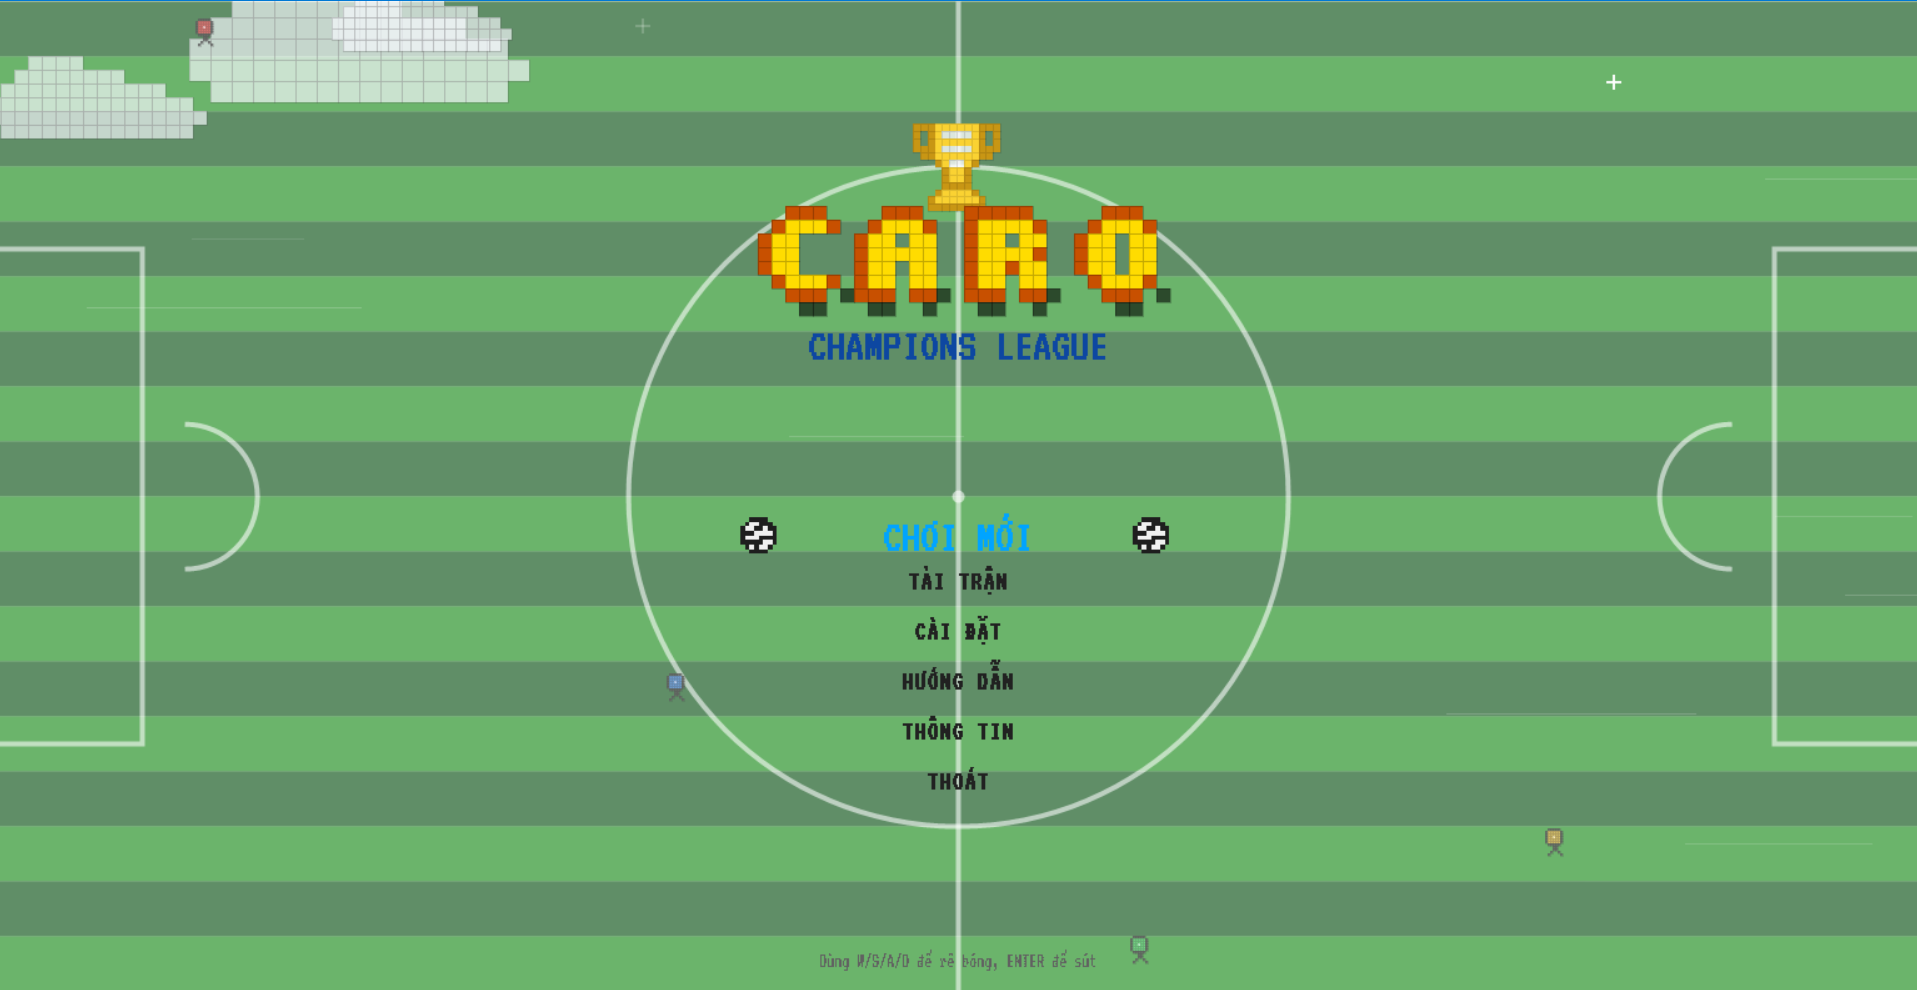
\includegraphics[width=0.9\linewidth]{images/ch4_menu.png}
\end{table}

\captionsetup{type=lstlisting}
\renewcommand{\arraystretch}{0.8}
\captionof{lstlisting}{Mã nguồn RenderMenuScreen và bố cục tiêu đề}\label{lst:ch4_menu_render}
\begin{longtable}{|>{\ttfamily\small\color{black}\raggedleft\arraybackslash}p{0.8cm}|>{\ttfamily\small\color{black}\arraybackslash}p{0.85\linewidth}|}
\hline
\normalfont\bfseries STT & \normalfont\bfseries Mã nguồn \\ \hline
1 & \cppkw{void} RenderMenuScreen(\cpptype{HDC} hdc, \cppkw{int} selectedOption, \cppkw{int} screenWidth, \cppkw{int} screenHeight) \\ \hline
2 & \{ \\ \hline
3 & \ \ Gdiplus::Graphics g(hdc); \\ \hline
4 & \ \ DrawProceduralStadium(g, screenWidth, screenHeight, true); \\ \hline
5 & \ \ Gdiplus::SolidBrush lightGlassBrush(Gdiplus::Color(80, 255, 255, 255)); \\ \hline
6 & \ \ g.FillRectangle(\&lightGlassBrush, 0, 0, screenWidth, screenHeight); \\ \hline
7 &  \\ \hline
8 & \ \ \cppkw{int} cupYOffset = UIScaler::SY((\cppkw{int})(sin(g\_GlobalAnimTime * 2.5f) * 10.0f)); \\ \hline
9 & \ \ DrawPixelTrophy(g, screenWidth / 2, screenHeight / 4 - UIScaler::SY(85) + cupYOffset, UIScaler::S(100)); \\ \hline
10 &  \\ \hline
11 & \ \ \cppkw{static} \cpptype{PixelModel} titleModel; \\ \hline
12 & \ \ \cppkw{static} std::map<int, Gdiplus::Color> titlePalette; \\ \hline
13 & \ \ \cppkw{if} (!titleModel.isLoaded) \{ \\ \hline
14 & \ \ \ \ titleModel = LoadPixelModel("Asset/models/bg/title\_caro.txt"); \\ \hline
15 & \ \ \ \ titlePalette[1] = ToGdiColor(Theme::TitleBorder); \\ \hline
16 & \ \ \ \ titlePalette[2] = ToGdiColor(Theme::TitleFill); \\ \hline
17 & \ \ \ \ titlePalette[3] = ToGdiColor(Theme::TitleShadow); \} \\ \hline
18 & \ \ DrawPixelModel(g, titleModel, screenWidth / 2, screenHeight / 4 + UIScaler::SY(20), UIScaler::S(500), titlePalette); \\ \hline
19 & \} \\ \hline
\end{longtable}

\subsection*{4.6.2. PlayScreen}
\addcontentsline{toc}{subsection}{\textcolor{black}{4.6.2. PlayScreen}}

\setlength{\parindent}{1.5em} PlayScreen tập trung vào tính rõ ràng và phản hồi thị giác:
\begin{itemize}
  \item Lưới cờ vẽ bằng GDI để giữ sắc nét.
  \item Cursor neon đổi màu theo lượt (cam cho P1, cyan cho P2).
  \item Highlight nước đi cuối và chuỗi thắng với hiệu ứng pulse.
  \item Animation cầu thủ sử dụng \texttt{DrawPixelAction} (idle/run/win/sad).
\end{itemize}
\setlength{\parindent}{1.5em} Phần logic cập nhật thời gian và trạng thái cũng làm nền cho UI (đếm giờ, thông báo thắng).

\setlength{\parindent}{1.5em} Trên PlayScreen, các chuỗi hiển thị như \texttt{play\_format} và \texttt{play\_turn} được lấy qua \texttt{GetText} nhằm đảm bảo đa ngôn ngữ. Việc dựng text score theo \texttt{state->targetScore} và \texttt{state->isP1Turn} giúp UI luôn đồng bộ với PlayState.

\setlength{\parindent}{1.5em} Bố cục gồm hai tab trái/phải cho thông tin người chơi, ở giữa là bàn cờ. Kích thước bàn cờ được tính động theo vùng trống (min giữa chiều rộng và chiều cao trừ biên), sau đó quy đổi thành \texttt{cellSize}. Trên cùng là scoreboard và đồng hồ đếm thời gian dạng ``glass panel'' có viền phát sáng theo lượt.

\begin{table}[H]
\caption*{Hình 4.4: Hình minh họa PlayScreen}
\addcontentsline{lof}{figure}{Hình 4.4: Hình minh họa PlayScreen}
\centering
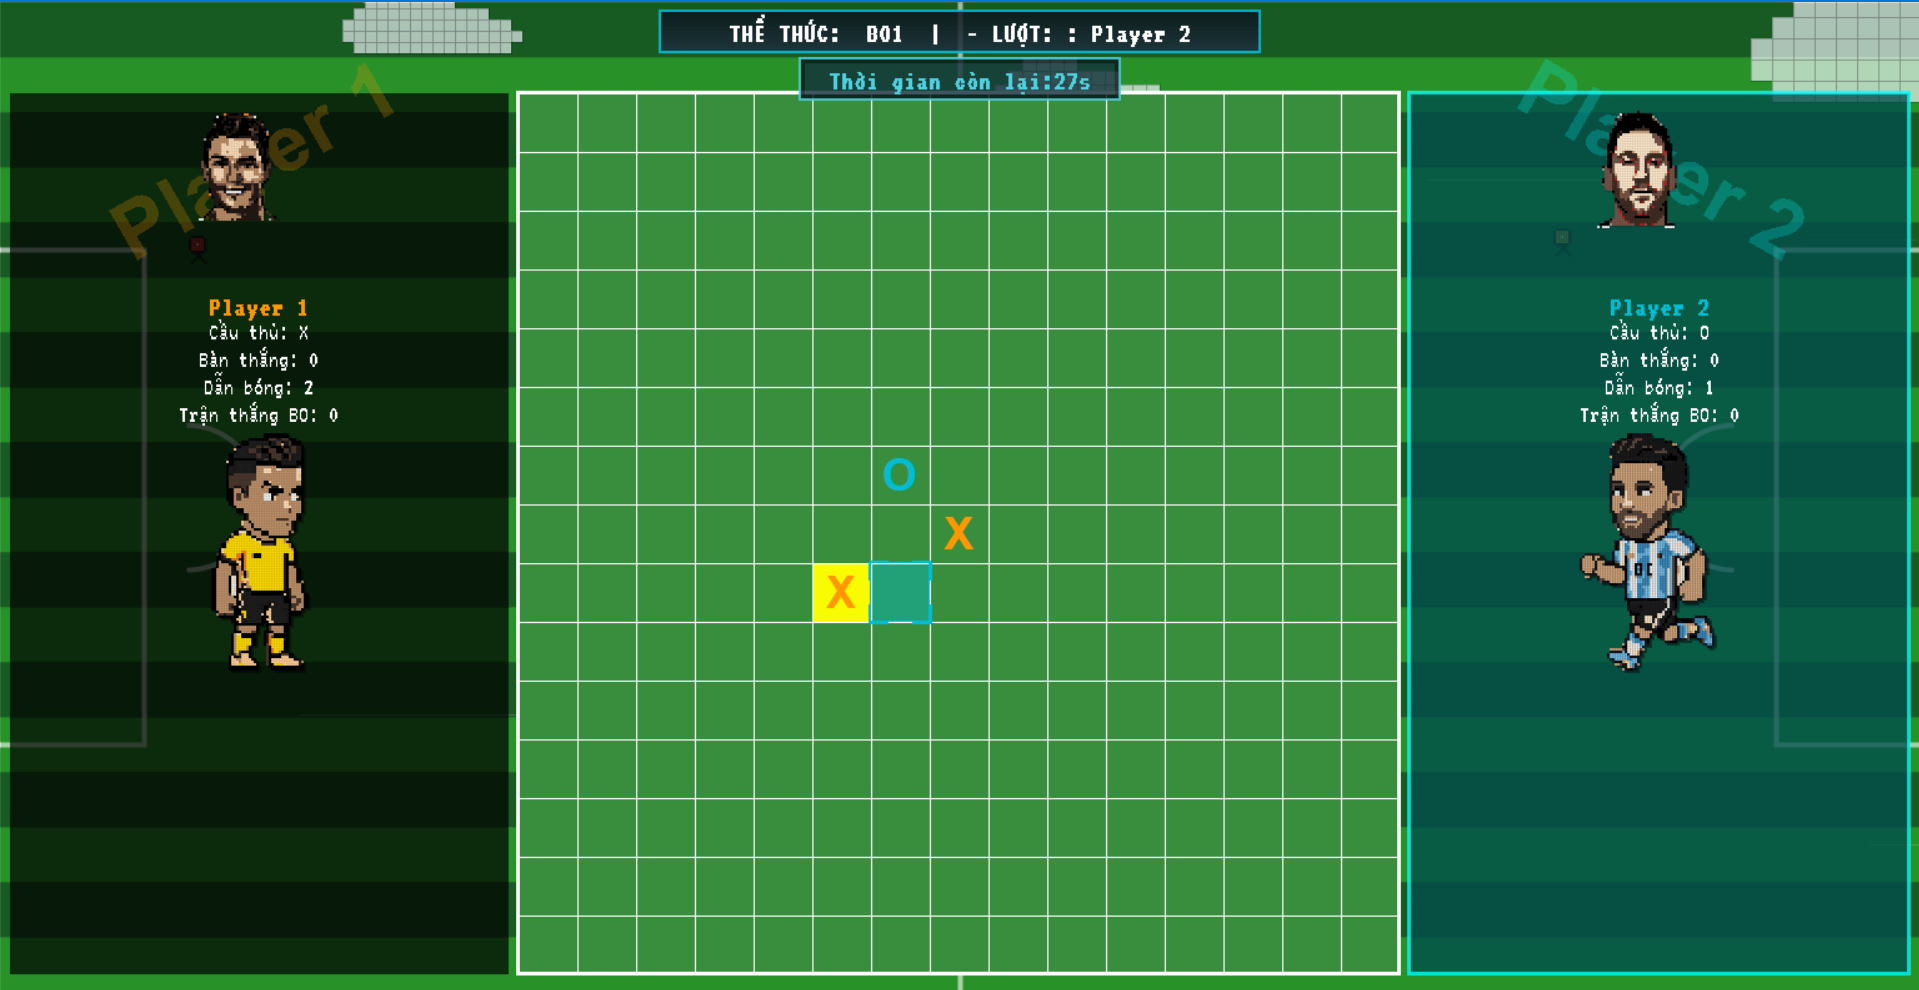
\includegraphics[width=0.9\linewidth]{images/ch4_play.png}
\end{table}

\captionsetup{type=lstlisting}
\renewcommand{\arraystretch}{0.8}
\captionof{lstlisting}{Mã nguồn RenderPlayScreen: tính kích thước và vẽ bàn cờ}\label{lst:ch4_play_render}
\begin{longtable}{|>{\ttfamily\small\color{black}\raggedleft\arraybackslash}p{0.8cm}|>{\ttfamily\small\color{black}\arraybackslash}p{0.85\linewidth}|}
\hline
\normalfont\bfseries STT & \normalfont\bfseries Mã nguồn \\ \hline
1 & \cppkw{void} RenderPlayScreen(\cpptype{HDC} hdc, \cppkw{const} \cpptype{PlayState} *state, \cppkw{int} screenWidth, \cppkw{int} screenHeight, \cppkw{const} \cpptype{GameConfig} *config) \\ \hline
2 & \{ \\ \hline
3 & \ \ Gdiplus::Graphics g(hdc); \\ \hline
4 & \ \ DrawProceduralStadium(g, screenWidth, screenHeight); \\ \hline
5 &  \\ \hline
6 & \ \ \cppkw{int} availableHeight = screenHeight - UIScaler::SY(120); \\ \hline
7 & \ \ \cppkw{int} availableWidth = screenWidth - UIScaler::SX(300); \\ \hline
8 & \ \ \cppkw{int} maxBoardSize = availableWidth < availableHeight ? availableWidth : availableHeight; \\ \hline
9 & \ \ \cppkw{int} dynamicCellSize = maxBoardSize / state->boardSize; \\ \hline
10 & \ \ \cppkw{int} boardPixelSize = state->boardSize * dynamicCellSize; \\ \hline
11 & \ \ \cppkw{int} startX = (screenWidth - boardPixelSize) / 2; \\ \hline
12 & \ \ \cppkw{int} startY = (screenHeight - boardPixelSize) / 2 + UIScaler::SY(40); \\ \hline
13 &  \\ \hline
14 & \ \ DrawGameBoard(g, hdc, state, dynamicCellSize, startX, startY); \\ \hline
15 &  \\ \hline
16 & \ \ \cppkw{int} scoreW = UIScaler::SX(600); \\ \hline
17 & \ \ \cppkw{int} scoreH = UIScaler::SY(45); \\ \hline
18 & \ \ \cppkw{int} scoreX = (screenWidth - scoreW) / 2; \\ \hline
19 & \ \ \cppkw{int} scoreY = UIScaler::SY(10); \\ \hline
20 & \ \ std::wstring formatText = GetText("play\_format") + L" BO" + std::to\_wstring(state->targetScore); \\ \hline
21 & \ \ std::wstring turnText = GetText("play\_turn") + L": " + (state->isP1Turn ? state->p1.name : state->p2.name); \\ \hline
22 & \ \ std::wstring fullScoreText = formatText + L"  |  " + turnText; \\ \hline
23 & \ \ COLORREF turnColor = state->isP1Turn ? ToCOLORREF(Palette::OrangeNormal) : ToCOLORREF(Palette::CyanNormal); \\ \hline
24 & \ \ \cppkw{float} pulseScore = 0.6f + sin(g\_GlobalAnimTime * 6.0f) * 0.4f; \\ \hline
25 & \ \ BYTE scoreAlpha = (BYTE)(130 + pulseScore * 125); \\ \hline
26 & \ \ Gdiplus::LinearGradientBrush scoreBg(Gdiplus::Point(scoreX, scoreY), Gdiplus::Point(scoreX, scoreY + scoreH), Gdiplus::Color(210, 10, 15, 25), Gdiplus::Color(210, 30, 45, 65)); \\ \hline
27 & \ \ g.FillRectangle(\&scoreBg, scoreX, scoreY, scoreW, scoreH); \\ \hline
28 & \ \ Gdiplus::Pen scoreBorder(Gdiplus::Color(scoreAlpha, GetRValue(turnColor), GetGValue(turnColor), GetBValue(turnColor)), 2.5f); \\ \hline
29 & \ \ g.DrawRectangle(\&scoreBorder, scoreX, scoreY, scoreW, scoreH); \\ \hline
30 & \} \\ \hline
\end{longtable}

\subsection*{4.6.3. Pause Game}
\addcontentsline{toc}{subsection}{\textcolor{black}{4.6.3. Pause Game}}

\setlength{\parindent}{1.5em} Pause menu là lớp phủ trực tiếp lên gameplay, nhằm giữ ngữ cảnh trong khi vẫn giảm độ tập trung vào bàn cờ. Màn hình gồm hai khối chính: khung menu bên trái và cột hướng dẫn điều khiển bên phải. Các mục như Resume, BGM, Volume, Save, Exit được trình bày theo danh sách dọc, trong đó volume có thanh trượt trực quan.

\setlength{\parindent}{1.5em} Lớp overlay dùng \texttt{Theme::GlassWhite} để giảm độ tương phản nền, tạo hiệu ứng "mờ" nhưng không làm mất hoàn toàn bối cảnh game. Điều này giúp người chơi vẫn nhận biết trạng thái ván đang tạm dừng.

\setlength{\parindent}{1.5em} Khi tạm dừng, hệ thống dùng nền kính trắng mờ để giảm nhiễu thị giác; banner ``Pause'' và icon còi (whistle) được vẽ bằng pixel art để giữ đồng nhất phong cách.

\begin{table}[H]
\caption*{Hình 4.5: Hình minh họa Pause Game}
\addcontentsline{lof}{figure}{Hình 4.5: Hình minh họa Pause Game}
\centering
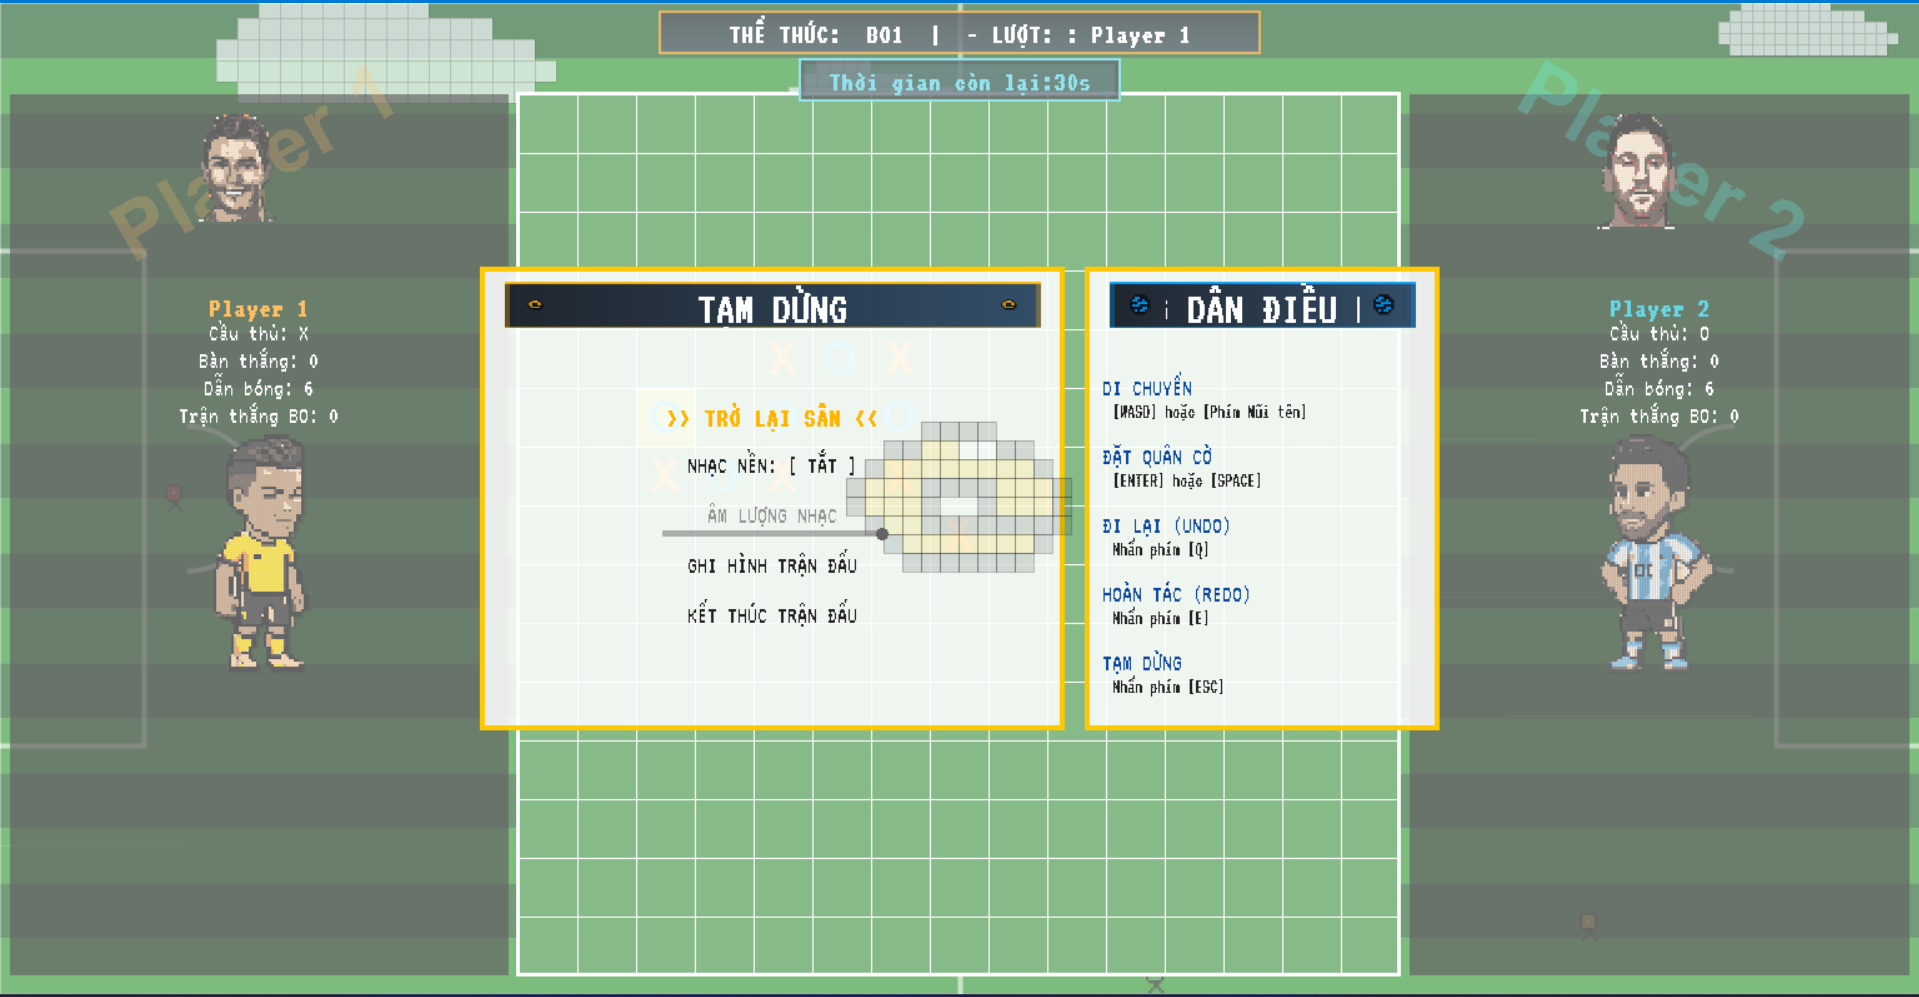
\includegraphics[width=0.9\linewidth]{images/ch4_pause.png}
\end{table}

\captionsetup{type=lstlisting}
\renewcommand{\arraystretch}{0.8}
\captionof{lstlisting}{Mã nguồn Lớp phủ Pause Menu trong RenderPlayScreen}\label{lst:ch4_pause_render}
\begin{longtable}{|>{\ttfamily\small\color{black}\raggedleft\arraybackslash}p{0.8cm}|>{\ttfamily\small\color{black}\arraybackslash}p{0.85\linewidth}|}
\hline
\normalfont\bfseries STT & \normalfont\bfseries Mã nguồn \\ \hline
1 & \cppkw{if} (state->status == MATCH\_PAUSED) \\ \hline
2 & \{ \\ \hline
3 & \ \ \cpptype{Gdiplus::SolidBrush} shadowBrush2(Gdiplus::Color(100, 255, 255, 255)); \\ \hline
4 & \ \ g.FillRectangle(\&shadowBrush2, 0, 0, screenWidth, screenHeight); \\ \hline
5 &  \\ \hline
6 & \ \ \cppkw{int} menuW = UIScaler::SX(580), menuH = UIScaler::SY(500); \\ \hline
7 & \ \ \cppkw{int} guideW = UIScaler::SX(350); \\ \hline
8 & \ \ \cppkw{int} gap = UIScaler::SX(25); \\ \hline
9 & \ \ \cppkw{int} totalW = (g\_CurrentSubMenu == SUB\_MAIN) ? (menuW + gap + guideW) : menuW; \\ \hline
10 & \ \ \cppkw{int} totalStartX = (screenWidth - totalW) / 2; \\ \hline
11 &  \\ \hline
12 & \ \ \cppkw{int} menuX = totalStartX; \\ \hline
13 & \ \ \cppkw{int} menuY = (screenHeight - menuH) / 2; \\ \hline
14 & \ \ \cpptype{Gdiplus::SolidBrush} bgBrush(ToGdiColor(Theme::GlassWhite)); \\ \hline
15 & \ \ g.FillRectangle(\&bgBrush, menuX, menuY, menuW, menuH); \\ \hline
16 & \ \ \cpptype{Gdiplus::Pen} yellowBorder(ToGdiColor(Theme::PanelYellowBorder), 4.0f); \\ \hline
17 & \ \ g.DrawRectangle(\&yellowBorder, menuX, menuY, menuW, menuH); \\ \hline
18 & \ \ DrawPixelBanner(g, hdc, GetText("pause\_title").c\_str(), menuX + menuW / 2, menuY + UIScaler::SY(40), menuW - UIScaler::SX(20), ToCOLORREF(Palette::White), RGB(255, 180, 0), "Asset/models/bg/whistle.txt"); \\ \hline
19 & \} \\ \hline
\end{longtable}

\subsection*{4.6.4. MatchConfigScreen}
\addcontentsline{toc}{subsection}{\textcolor{black}{4.6.4. MatchConfigScreen}}

\setlength{\parindent}{1.5em} Màn hình cấu hình trận đấu có hai trang, áp dụng UI điều hướng rõ ràng:
\begin{itemize}
  \item Trang 1: cấu hình chế độ, PvP/PvE, độ khó, thời gian, số ván.
  \item Trang 2: cấu hình avatar và tên người chơi với input trực tiếp.
\end{itemize}
\setlength{\parindent}{1.5em} Màu sắc và font thay đổi theo lựa chọn để nhấn mạnh mục đang focus; mỗi giá trị được hiển thị trong khung riêng, tạo cảm giác ``form'' rõ ràng.

\setlength{\parindent}{1.5em} Layout chính là một panel kính giữa màn hình, chia hai cột (nhãn và giá trị). Ở trang 2, mỗi người chơi là một ``card'' riêng với avatar, tên, và hiệu ứng glow khi đang được chọn.

\begin{table}[H]
\caption*{Hình 4.6: Hình minh họa MatchConfigScreen - trang 1}
\addcontentsline{lof}{figure}{Hình 4.6: Hình minh họa MatchConfigScreen - trang 1}
\centering
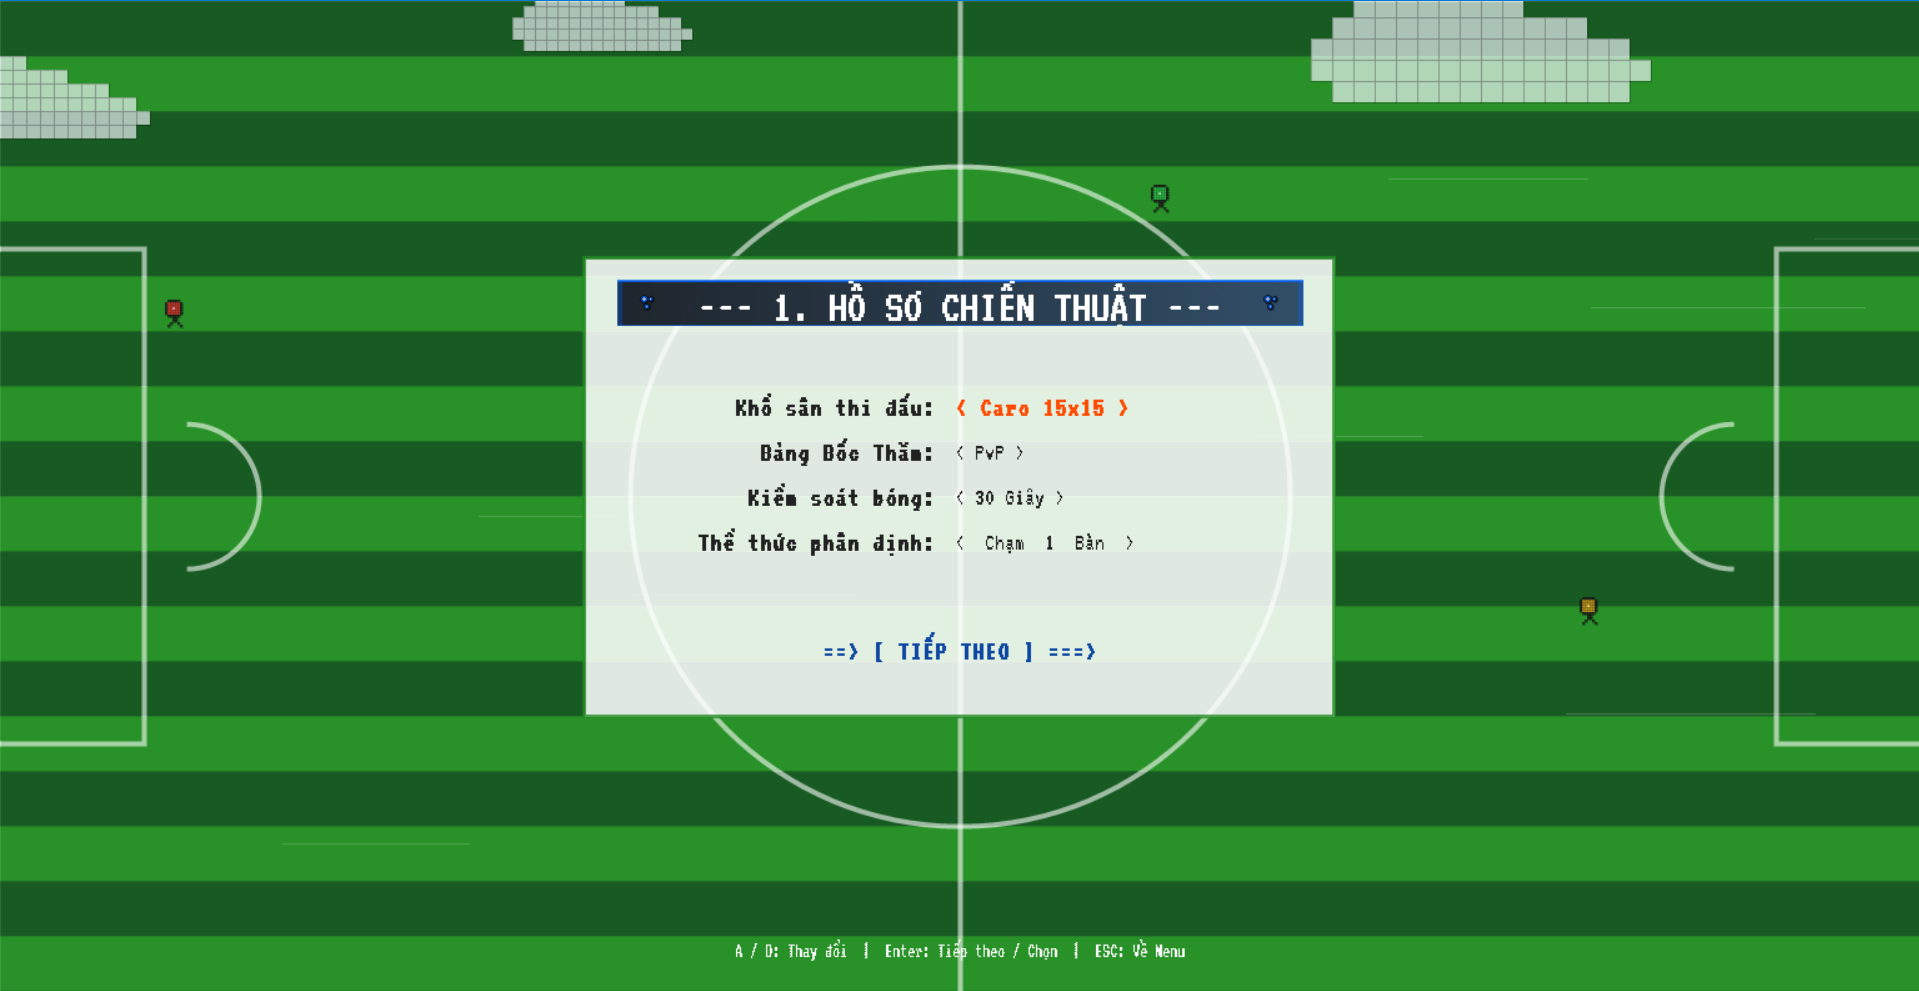
\includegraphics[width=0.9\linewidth]{images/ch4_match_config.png}
\end{table}

\begin{table}[H]
\caption*{Hình 4.7: Hình minh họa MatchConfigScreen - trang 2}
\addcontentsline{lof}{figure}{Hình 4.7: Hình minh họa MatchConfigScreen - trang 2}
\centering
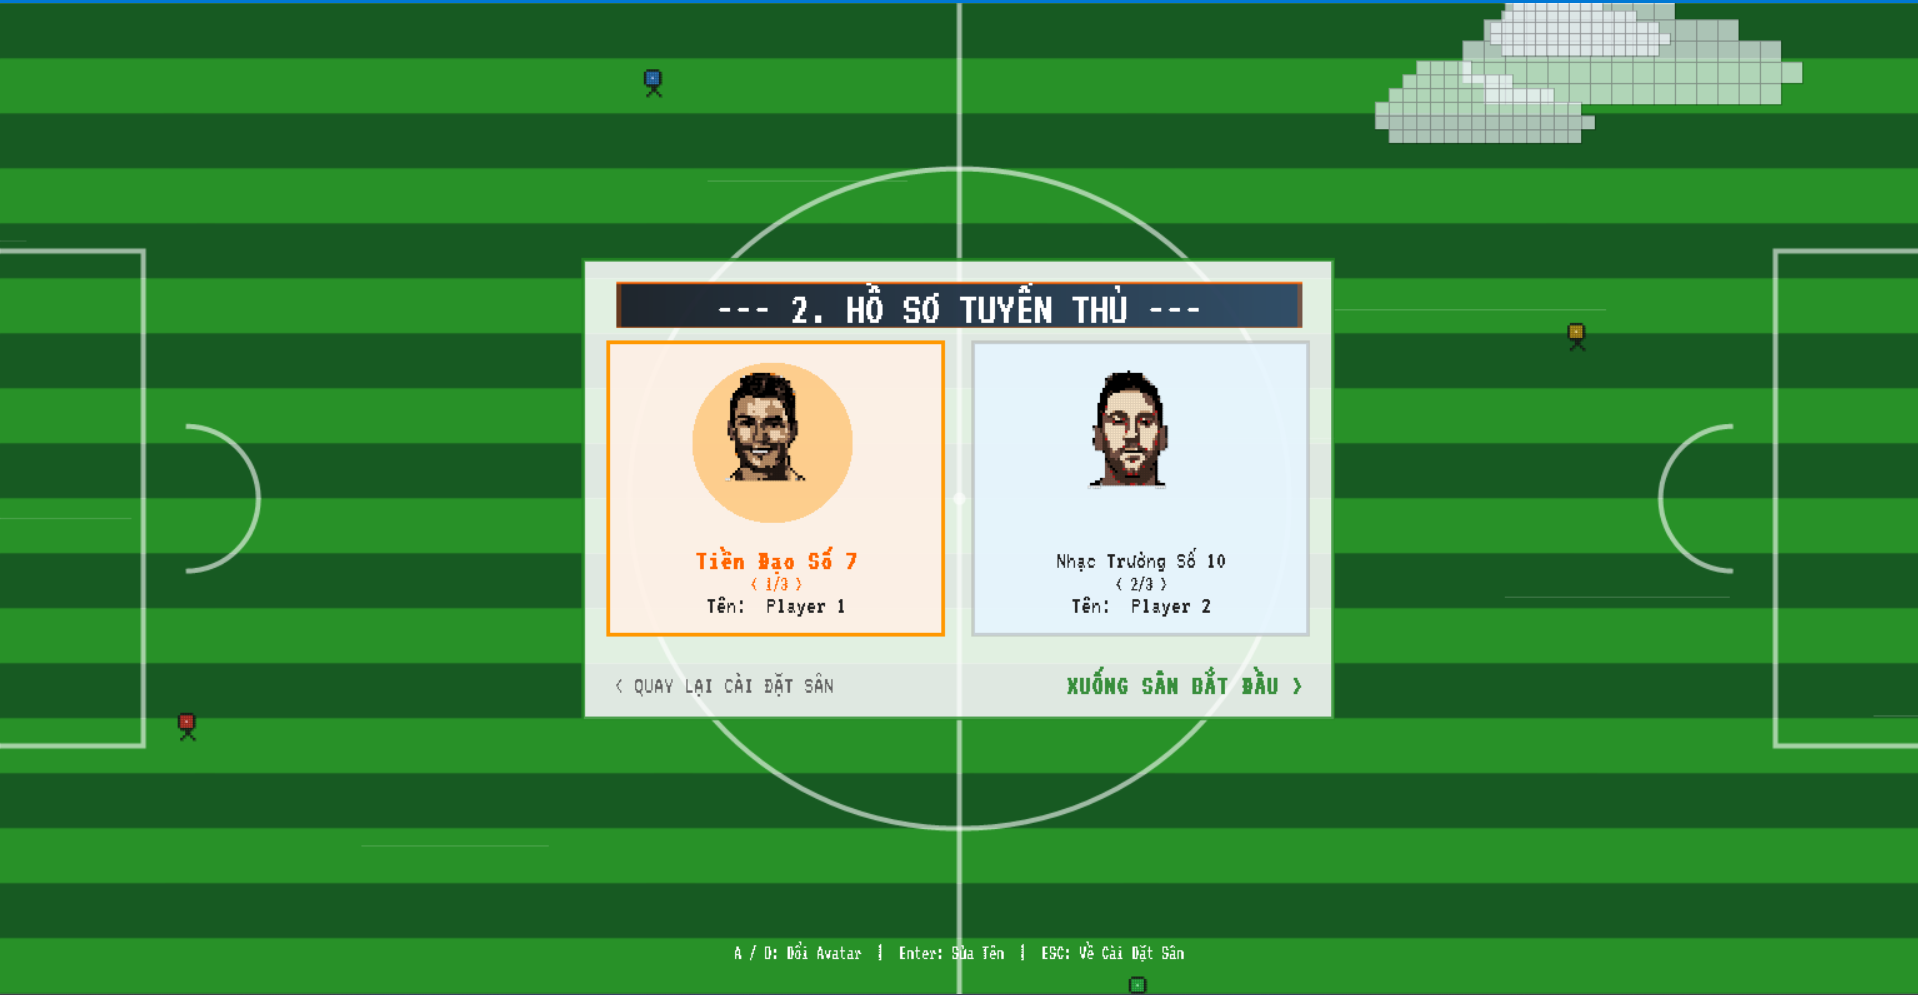
\includegraphics[width=0.9\linewidth]{images/ch4_match_config_2.png}
\end{table}

\captionsetup{type=lstlisting}
\renewcommand{\arraystretch}{0.8}
\captionof{lstlisting}{Mã nguồn RenderMatchConfigScreen: panel và banner}\label{lst:ch4_match_config_render}
\begin{longtable}{|>{\ttfamily\small\color{black}\raggedleft\arraybackslash}p{0.8cm}|>{\ttfamily\small\color{black}\arraybackslash}p{0.85\linewidth}|}
\hline
\normalfont\bfseries STT & \normalfont\bfseries Mã nguồn \\ \hline
1 & \cppkw{void} RenderMatchConfigScreen(\cpptype{HDC} hdc, \cppkw{int} selectedOption, \cppkw{const} \cpptype{PlayState} *config, \cppkw{int} screenWidth, \cppkw{int} screenHeight) \\ \hline
2 & \{ \\ \hline
3 & \ \ Gdiplus::Graphics g(hdc); \\ \hline
4 & \ \ DrawProceduralStadium(g, screenWidth, screenHeight); \\ \hline
5 &  \\ \hline
6 & \ \ Gdiplus::SolidBrush whitePanel(ToGdiColor(Theme::GlassWhite)); \\ \hline
7 & \ \ \cppkw{int} panelW = UIScaler::SX(750); \\ \hline
8 & \ \ \cppkw{int} panelH = UIScaler::SY(500); \\ \hline
9 & \ \ \cppkw{int} panelX = (screenWidth - panelW) / 2; \\ \hline
10 & \ \ \cppkw{int} panelY = (screenHeight - panelH) / 2 - UIScaler::SY(10); \\ \hline
11 & \ \ g.FillRectangle(\&whitePanel, panelX, panelY, panelW, panelH); \\ \hline
12 & \ \ Gdiplus::Pen panelPen(ToGdiColor(Theme::PanelGreenBorder), 3.0f); \\ \hline
13 & \ \ g.DrawRectangle(\&panelPen, panelX, panelY, panelW, panelH); \\ \hline
14 & \ \ DrawPixelBanner(g, hdc, GetText("config\_page1").c\_str(), screenWidth / 2, panelY + UIScaler::SY(50), panelW - UIScaler::SX(40), ToCOLORREF(Palette::White), RGB(0, 100, 255), "Asset/models/bg/gears.txt"); \\ \hline
15 & \} \\ \hline
\end{longtable}

\subsection*{4.6.5. SettingScreen}
\addcontentsline{toc}{subsection}{\textcolor{black}{4.6.5. SettingScreen}}

\setlength{\parindent}{1.5em} SettingScreen là ví dụ điển hình của layout dạng bảng và thanh trượt:
\begin{itemize}
  \item Panel kính trắng, viền màu xanh.
  \item Banner tiêu đề có icon bánh răng.
  \item Thanh volume vẽ bằng GDI+, có bar track, fill, thumb.
  \item Mục bị disable sẽ đổi màu xám để giảm độ nổi bật.
\end{itemize}
\setlength{\parindent}{1.5em} Các mục bật/tắt được trình bày dưới dạng nhãn trạng thái, trong khi thanh trượt thể hiện mức âm lượng bằng tỉ lệ chiều dài.

\setlength{\parindent}{1.5em} Hệ thống chia panel thành hai cột: nhãn (trái) và giá trị (phải). Thanh trượt âm lượng dùng GDI+ để vẽ nền, phần fill và thumb, đồng thời đổi màu khi mục đang được chọn.

\setlength{\parindent}{1.5em} Các màu của thanh trượt lấy từ \texttt{Theme::BarTrack}, \texttt{Theme::BarFillSelected} và \texttt{Theme::BarFillNormal}, giúp nhất quán với bảng màu tổng thể. Khi tắt BGM/SFX, màu mục chuyển xám để biểu đạt trạng thái disable.

\begin{table}[H]
\caption*{Hình 4.8: Hình minh họa SettingScreen}
\addcontentsline{lof}{figure}{Hình 4.8: Hình minh họa SettingScreen}
\centering
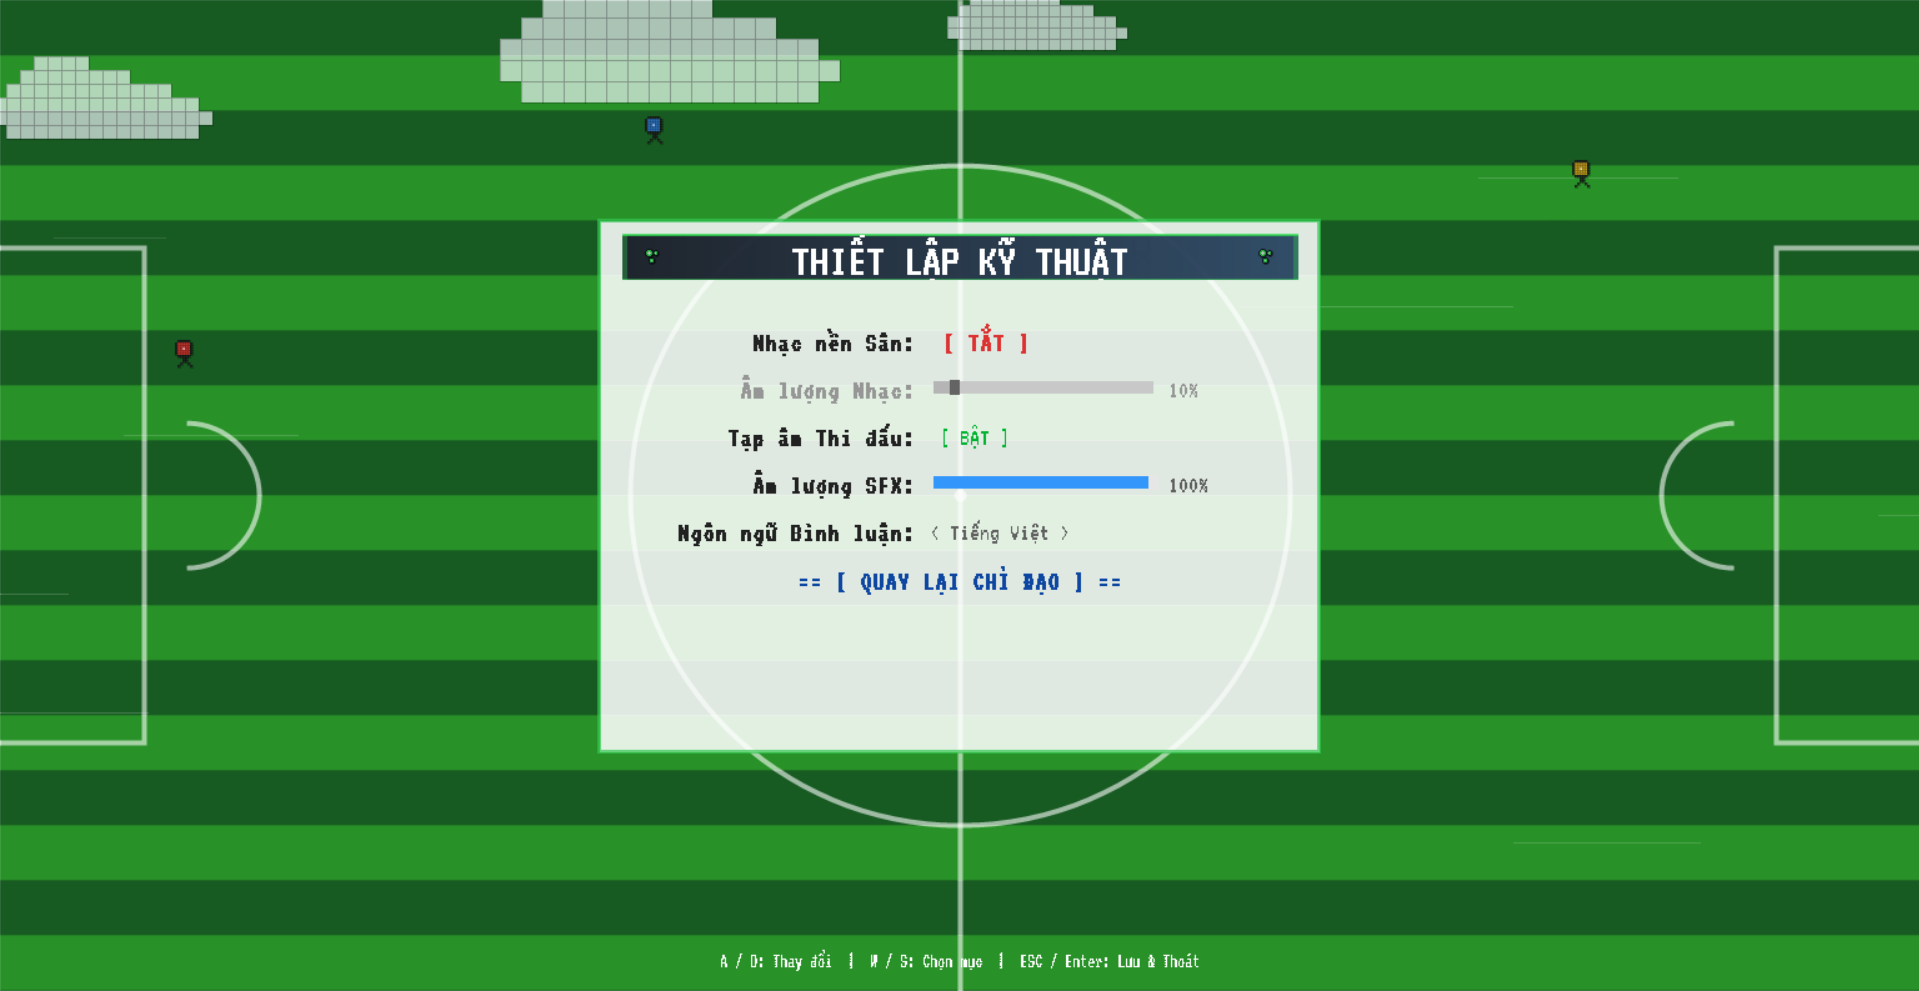
\includegraphics[width=0.9\linewidth]{images/ch4_setting.png}
\end{table}

\captionsetup{type=lstlisting}
\renewcommand{\arraystretch}{0.8}
\captionof{lstlisting}{Mã nguồn RenderSettingScreen: panel và thanh volume}\label{lst:ch4_setting_render}
\begin{longtable}{|>{\ttfamily\small\color{black}\raggedleft\arraybackslash}p{0.8cm}|>{\ttfamily\small\color{black}\arraybackslash}p{0.85\linewidth}|}
\hline
\normalfont\bfseries STT & \normalfont\bfseries Mã nguồn \\ \hline
1 & \cppkw{void} RenderSettingScreen(\cpptype{HDC} hdc, \cppkw{const} \cpptype{GameConfig} *config, \cppkw{int} selectedOption, \cppkw{int} screenWidth, \cppkw{int} screenHeight) \\ \hline
2 & \{ \\ \hline
3 & \ \ Gdiplus::Graphics g(hdc); \\ \hline
4 & \ \ DrawProceduralStadium(g, screenWidth, screenHeight); \\ \hline
5 &  \\ \hline
6 & \ \ \cppkw{int} panelW = UIScaler::SX(720); \\ \hline
7 & \ \ \cppkw{int} panelH = UIScaler::SY(580); \\ \hline
8 & \ \ \cppkw{int} panelX = (screenWidth - panelW) / 2; \\ \hline
9 & \ \ \cppkw{int} panelY = (screenHeight - panelH) / 2 - UIScaler::SY(10); \\ \hline
10 & \ \ Gdiplus::SolidBrush whitePanel(ToGdiColor(Theme::GlassWhite)); \\ \hline
11 & \ \ g.FillRectangle(\&whitePanel, panelX, panelY, panelW, panelH); \\ \hline
12 & \ \ DrawPixelBanner(g, hdc, GetText("setting\_title").c\_str(), screenWidth / 2, panelY + UIScaler::SY(40), panelW - UIScaler::SX(20), ToCOLORREF(Palette::White), RGB(50, 220, 80), "Asset/models/bg/gears.txt"); \\ \hline
13 & \} \\ \hline
\end{longtable}

\subsection*{4.6.6. LoadGameScreen}
\addcontentsline{toc}{subsection}{\textcolor{black}{4.6.6. LoadGameScreen}}

\setlength{\parindent}{1.5em} Màn hình load game chia thành ba vùng: danh sách slot, thông tin slot, và hành động. Trạng thái tương tác được quản lý rõ ràng:
\begin{itemize}
  \item \texttt{MODE\_SELECT\_SLOT}: chọn slot ở cột trái.
  \item \texttt{MODE\_SELECT\_ACTION}: chọn hành động (Load/Rename/Delete/Back).
  \item \texttt{MODE\_EDIT\_NAME}: nhập tên slot mới.
\end{itemize}
\setlength{\parindent}{1.5em} Điểm UX quan trọng: nếu slot trống sẽ hiển thị thông báo ngắn, tránh thao tác không cần thiết. Các panel được chia cột bằng layout tính theo \texttt{UIScaler} nên luôn cân đối.

\setlength{\parindent}{1.5em} Màn hình gồm ba cột: danh sách slot, thông tin chi tiết và cột hành động/đổi tên. Trạng thái chọn được tô nền bằng màu trong suốt để phân biệt giữa ``đang chọn slot'' và ``đang chọn hành động''.

\setlength{\parindent}{1.5em} Các màu nhấn cho slot lấy từ \texttt{Theme::SlotSelected} và \texttt{Theme::SlotNormal}, đảm bảo đồng bộ với palette chung. Đây là chi tiết nhỏ nhưng giúp UI không bị "lạc tông" giữa các màn hình.

\begin{table}[H]
\caption*{Hình 4.9: Hình minh họa LoadGameScreen}
\addcontentsline{lof}{figure}{Hình 4.9: Hình minh họa LoadGameScreen}
\centering
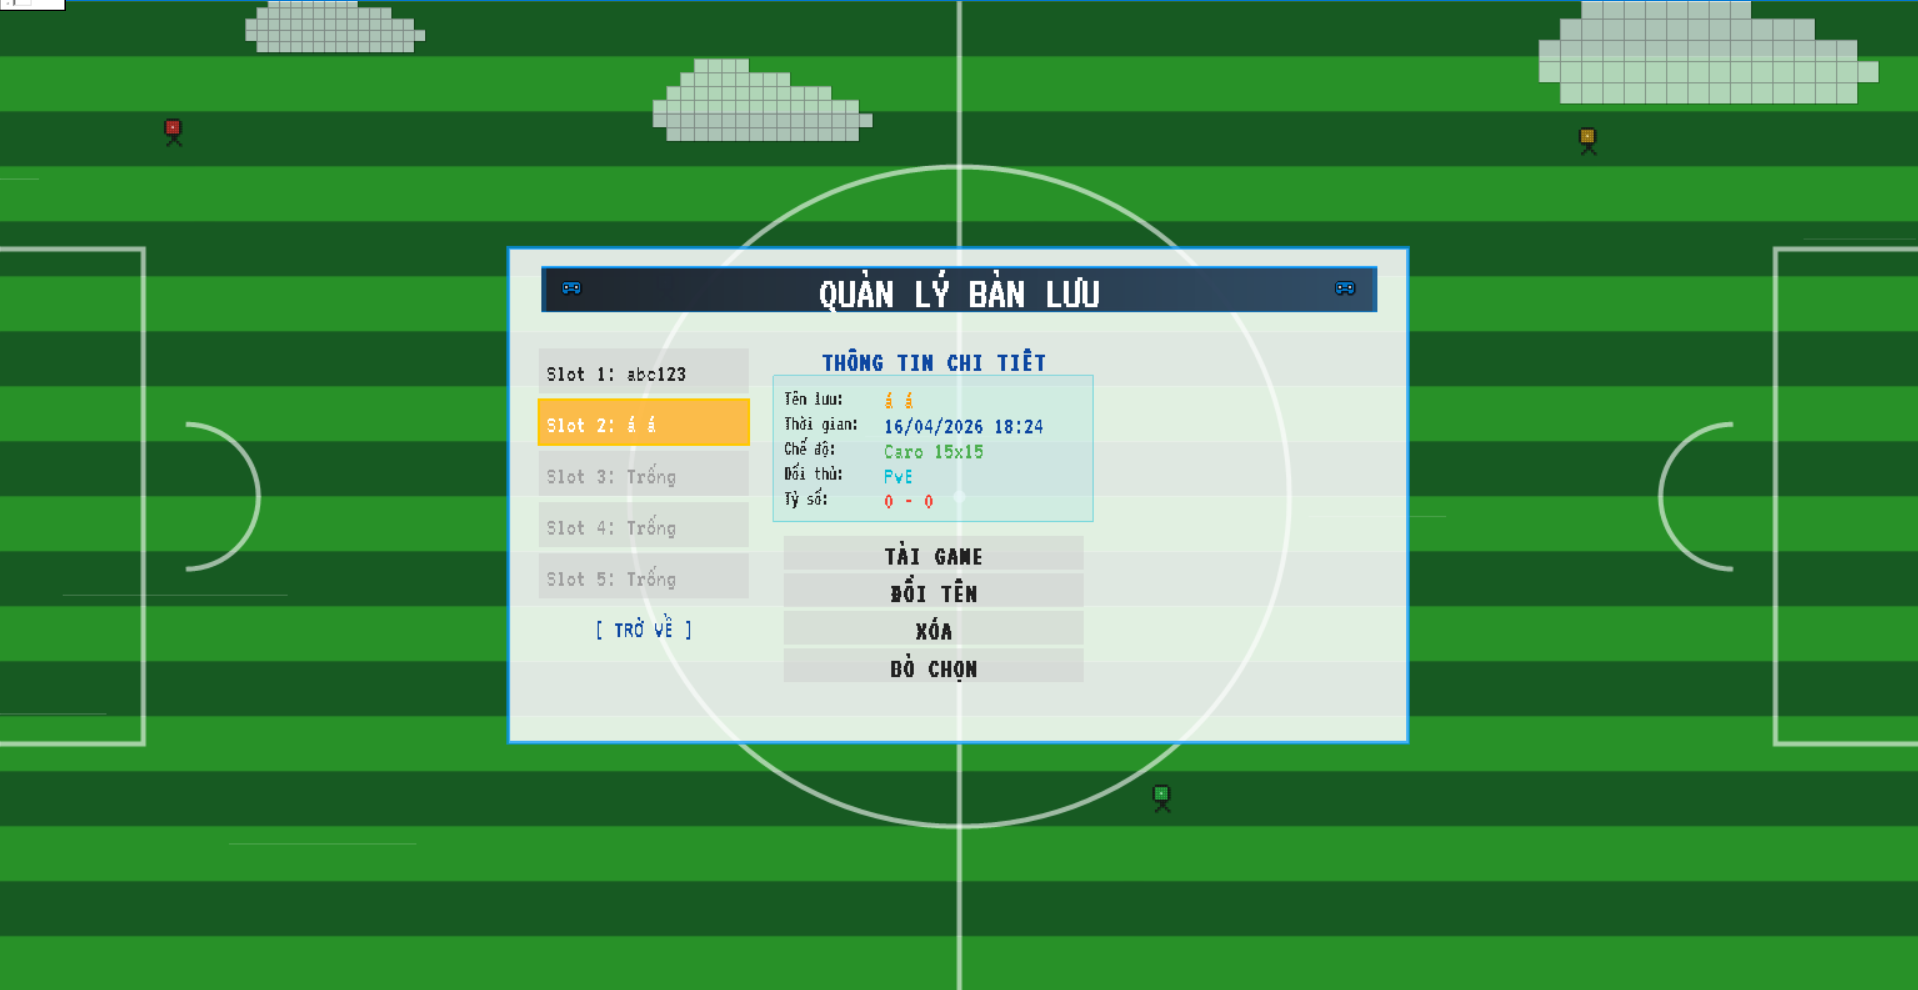
\includegraphics[width=0.9\linewidth]{images/ch4_load_game.png}
\end{table}

\captionsetup{type=lstlisting}
\renewcommand{\arraystretch}{0.8}
\captionof{lstlisting}{Mã nguồn Che do tuong tac va RenderLoadGameScreen}\label{lst:ch4_load_render}
\begin{longtable}{|>{\ttfamily\small\color{black}\raggedleft\arraybackslash}p{0.8cm}|>{\ttfamily\small\color{black}\arraybackslash}p{0.85\linewidth}|}
\hline
\normalfont\bfseries STT & \normalfont\bfseries Mã nguồn \\ \hline
1 & \cppkw{enum} LoadScreenMode \\ \hline
2 & \{ MODE\_SELECT\_SLOT, MODE\_SELECT\_ACTION, MODE\_EDIT\_NAME \}; \\ \hline
3 &  \\ \hline
4 & \cppkw{void} RenderLoadGameScreen(\cpptype{HDC} hdc, \cppkw{int} selectedOption, \cppkw{const} \cpptype{std::wstring} \&statusMessage, \cppkw{int} screenWidth, \cppkw{int} screenHeight) \\ \hline
5 & \{ \\ \hline
6 & \ \ Gdiplus::Graphics g(hdc); \\ \hline
7 & \ \ DrawProceduralStadium(g, screenWidth, screenHeight); \\ \hline
8 &  \\ \hline
9 & \ \ \cppkw{int} panelW = UIScaler::SX(900); \\ \hline
10 & \ \ \cppkw{int} panelH = UIScaler::SY(540); \\ \hline
11 & \ \ \cppkw{int} panelX = (screenWidth - panelW) / 2; \\ \hline
12 & \ \ \cppkw{int} panelY = (screenHeight - panelH) / 2; \\ \hline
13 & \ \ Gdiplus::SolidBrush bgBrush(ToGdiColor(Theme::GlassWhite)); \\ \hline
14 & \ \ g.FillRectangle(\&bgBrush, panelX, panelY, panelW, panelH); \\ \hline
15 & \ \ DrawPixelBanner(g, hdc, GetText("save\_title").c\_str(), screenWidth / 2, panelY + UIScaler::SY(45), panelW - UIScaler::SX(40), ToCOLORREF(Palette::White), RGB(0, 150, 255), "Asset/models/bg/cassette.txt"); \\ \hline
16 & \} \\ \hline
\end{longtable}

\subsection*{4.6.7. AboutScreen}
\addcontentsline{toc}{subsection}{\textcolor{black}{4.6.7. AboutScreen}}

\setlength{\parindent}{1.5em} AboutScreen thể hiện phong cách trình bày thông tin:
\begin{itemize}
  \item Nền sân + lớp kính mờ.
  \item Banner tiêu đề theo ngôn ngữ.
  \item Bảng thành viên với header nền xanh, grid line rõ ràng.
  \item Dòng giảng viên hướng dẫn và công nghệ.
\end{itemize}
\setlength{\parindent}{1.5em} Màu sắc thiên sáng, thể hiện tông sáng nhẹ nhàng hơn so với các màn hình gameplay.

\setlength{\parindent}{1.5em} Bảng thành viên được vẽ như một bảng dữ liệu: có header nền xanh, chia cột, kẻ grid line bằng GDI+ để đảm bảo độ đều. Các dòng chữ căn giữa theo từng cột.

\begin{table}[H]
\caption*{Hình 4.10: Hình minh họa AboutScreen}
\addcontentsline{lof}{figure}{Hình 4.10: Hình minh họa AboutScreen}
\centering
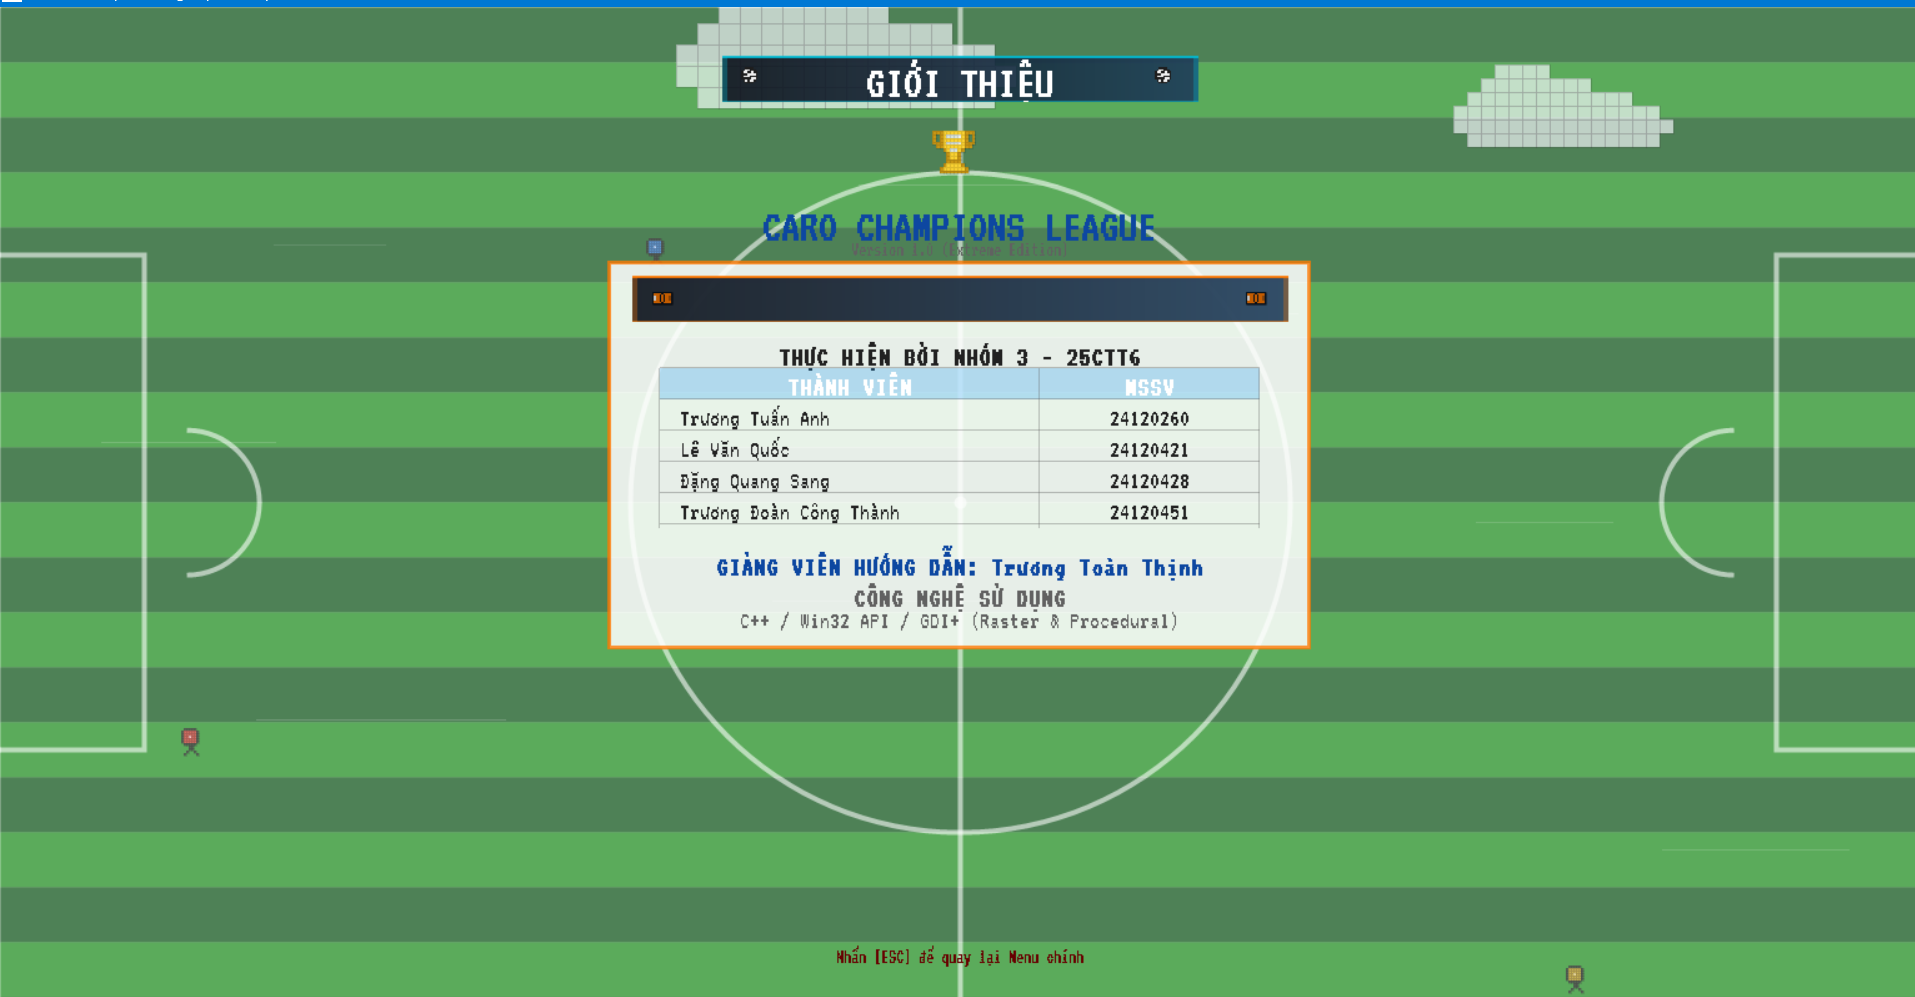
\includegraphics[width=0.9\linewidth]{images/ch4_about.png}
\end{table}

\captionsetup{type=lstlisting}
\renewcommand{\arraystretch}{0.8}
\captionof{lstlisting}{Mã nguồn RenderAboutScreen: banner va bang thanh vien}\label{lst:ch4_about_render}
\begin{longtable}{|>{\ttfamily\small\color{black}\raggedleft\arraybackslash}p{0.8cm}|>{\ttfamily\small\color{black}\arraybackslash}p{0.85\linewidth}|}
\hline
\normalfont\bfseries STT & \normalfont\bfseries Mã nguồn \\ \hline
1 & \cppkw{void} RenderAboutScreen(\cpptype{HDC} hdc, \cppkw{int} screenWidth, \cppkw{int} screenHeight) \\ \hline
2 & \{ \\ \hline
3 & \ \ Gdiplus::Graphics g(hdc); \\ \hline
4 & \ \ DrawProceduralStadium(g, screenWidth, screenHeight); \\ \hline
5 & \ \ DrawPixelBanner(g, hdc, GetText("about\_title").c\_str(), screenWidth / 2, UIScaler::SY(80), UIScaler::SX(500), ToCOLORREF(Palette::White), ToCOLORREF(Palette::CyanNormal)); \\ \hline
6 &  \\ \hline
7 & \ \ \cppkw{int} tableW = UIScaler::SX(600); \\ \hline
8 & \ \ \cppkw{int} tableH = UIScaler::SY(175); \\ \hline
9 & \ \ \cppkw{int} tableX = (screenWidth - tableW) / 2; \\ \hline
10 & \ \ \cppkw{int} tableY = UIScaler::SY(395); \\ \hline
11 & \ \ Gdiplus::Pen gridPen(Gdiplus::Color(100, 100, 100, 100), 1.0f); \\ \hline
12 & \ \ g.DrawLine(\&gridPen, (INT)tableX, (INT)tableY, (INT)(tableX + tableW), (INT)tableY); \\ \hline
13 & \} \\ \hline
\end{longtable}

\subsection*{4.6.8. GuildScreen}
\addcontentsline{toc}{subsection}{\textcolor{black}{4.6.8. GuildScreen}}

\setlength{\parindent}{1.5em} GuildScreen chia thành 3 trang hướng dẫn, có chấm phân trang và mũi tên điều hướng:
\begin{itemize}
  \item Trang 1: so sánh Caro và TicTacToe (hai cột).
  \item Trang 2: hướng dẫn di chuyển và thao tác.
  \item Trang 3: giải thích hệ thống AI, thời gian, mục tiêu, lưu trận.
\end{itemize}
\setlength{\parindent}{1.5em} Điểm nhấn UX là phân trang bằng dot + aura, giúp người dùng biết mình đang ở đâu trong chuỗi hướng dẫn.

\setlength{\parindent}{1.5em} Tiêu đề và màu banner thay đổi theo trang (cam, cyan, xanh lá), đồng thời hệ thống hiển thị mũi tên điều hướng ở hai bên để gợi ý thao tác.

\begin{table}[H]
\caption*{Hình 4.11: Hình minh họa GuildScreen}
\addcontentsline{lof}{figure}{Hình 4.11: Hình minh họa GuildScreen}
\centering
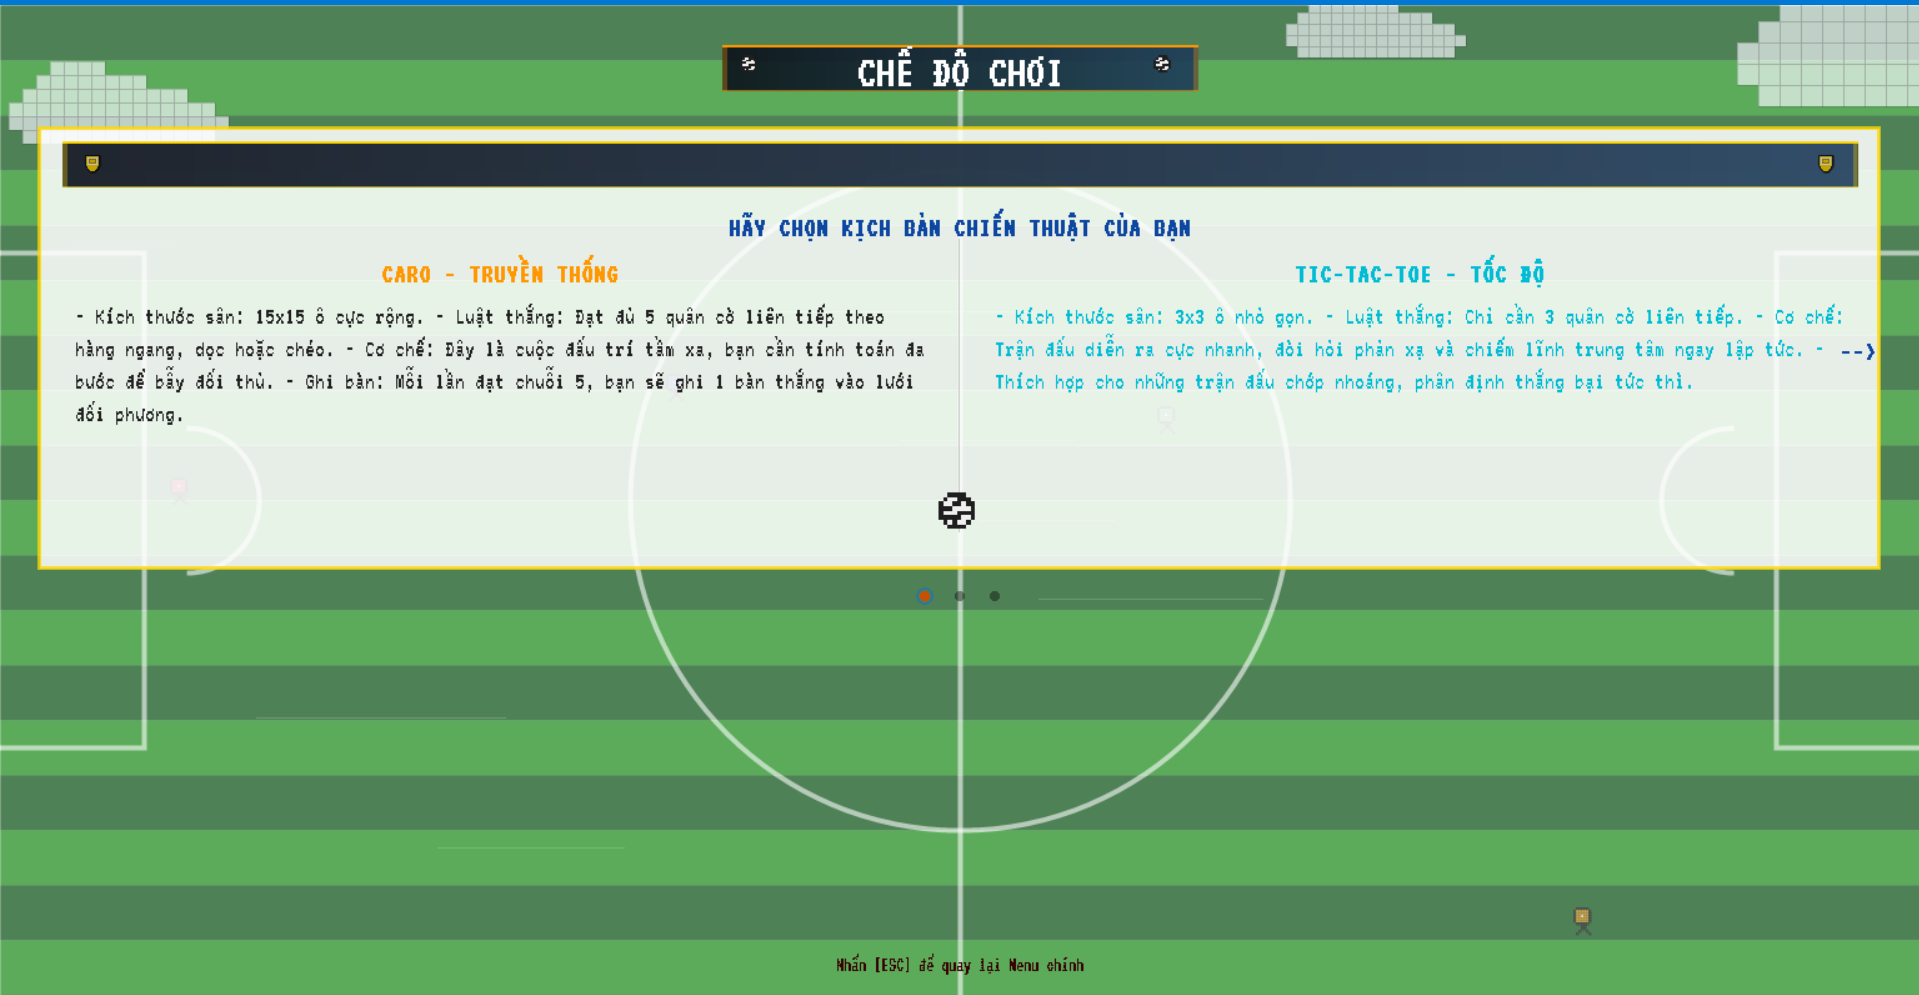
\includegraphics[width=0.9\linewidth]{images/ch4_guild.png}
\end{table}

\captionsetup{type=lstlisting}
\renewcommand{\arraystretch}{0.8}
\captionof{lstlisting}{Mã nguồn RenderGuildScreen: banner va phan trang}\label{lst:ch4_guild_render}
\begin{longtable}{|>{\ttfamily\small\color{black}\raggedleft\arraybackslash}p{0.8cm}|>{\ttfamily\small\color{black}\arraybackslash}p{0.85\linewidth}|}
\hline
\normalfont\bfseries STT & \normalfont\bfseries Mã nguồn \\ \hline
1 & \cppkw{void} RenderGuildScreen(\cpptype{HDC} hdc, \cppkw{int} screenWidth, \cppkw{int} screenHeight, \cppkw{int} currentPage) \\ \hline
2 & \{ \\ \hline
3 & \ \ Gdiplus::Graphics g(hdc); \\ \hline
4 & \ \ DrawProceduralStadium(g, screenWidth, screenHeight); \\ \hline
5 & \ \ COLORREF bannerColors[] = \{ ToCOLORREF(Palette::OrangeNormal), ToCOLORREF(Palette::CyanNormal), ToCOLORREF(Palette::GreenNormal) \}; \\ \hline
6 & \ \ std::wstring titles[] = \{ GetText("guild\_tab1"), GetText("guild\_tab2"), GetText("guild\_tab3") \}; \\ \hline
7 & \ \ DrawPixelBanner(g, hdc, titles[currentPage].c\_str(), screenWidth / 2, UIScaler::SY(70), UIScaler::SX(500), ToCOLORREF(Palette::White), bannerColors[currentPage]); \\ \hline
8 & \} \\ \hline
\end{longtable}

\subsection*{4.6.9. SaveGameScreen}
\addcontentsline{toc}{subsection}{\textcolor{black}{4.6.9. SaveGameScreen}}

\setlength{\parindent}{1.5em} SaveGameScreen có layout tương tự LoadGameScreen nhưng ưu tiên thao tác ghi dữ liệu. Màn hình chia thành ba vùng: danh sách slot, thông tin slot đang chọn, và vùng nhập tên bản lưu. UX mục tiêu là giảm thao tác nhầm: slot trống sẽ hiển thị nhãn "Empty" rõ ràng, slot đã có sẽ hiển thị tên + thời gian lưu gần nhất.

\setlength{\parindent}{1.5em} Khung nhập tên dùng \texttt{Theme::SaveBoxBorder} để tạo viền cam, giúp người chơi nhận biết vùng focus. Tên được giới hạn độ dài ở tầng lưu dữ liệu, nên UI có thể hiển thị thông báo nếu vượt quá giới hạn mà không làm lỗi file.

\setlength{\parindent}{1.5em} Ở chế độ nhập tên, vùng input được tô viền nổi và con trỏ nhấp nháy, đảm bảo người chơi nhận biết trạng thái đang nhập. Khi lưu thành công, thông báo trạng thái hiển thị ngắn ở góc dưới để xác nhận mà không phá bố cục.

\begin{figure}[H]
  \addcontentsline{lof}{figure}{Hình 4.12: Hình minh họa SaveGameScreen}
\centering
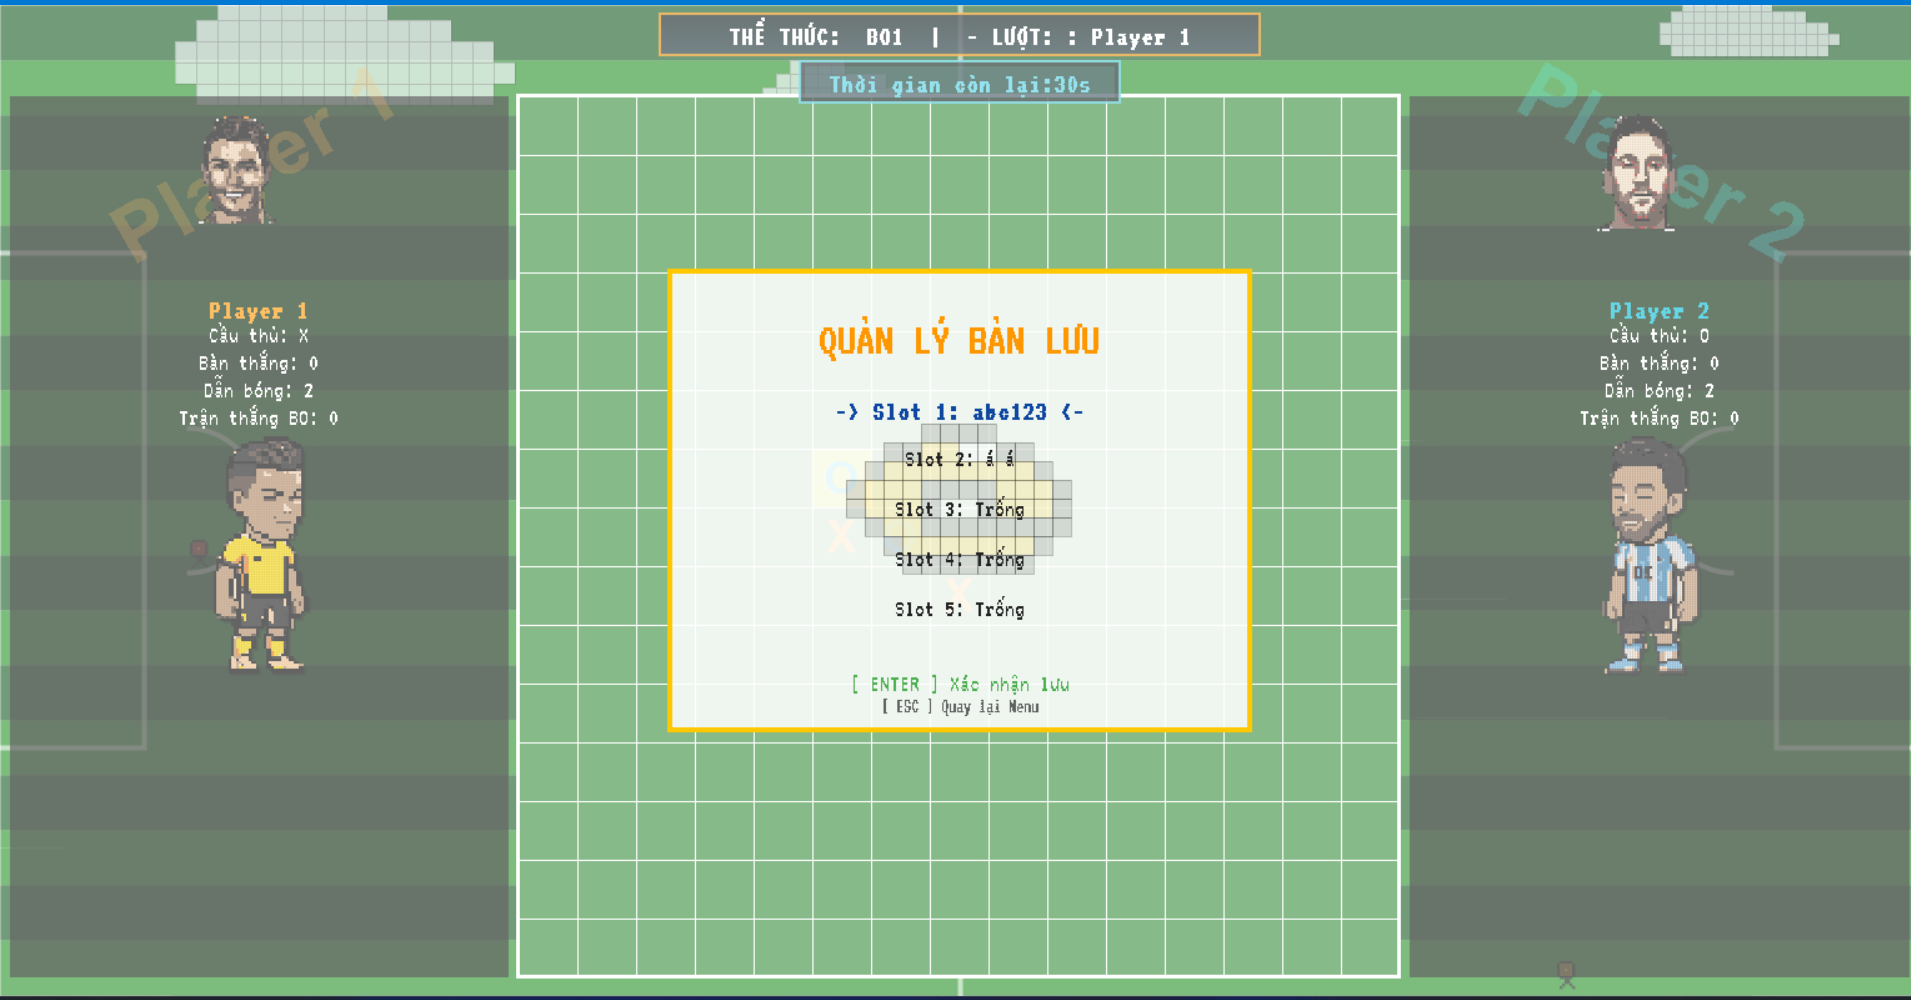
\includegraphics[width=0.45\linewidth]{images/ch4_save_game.png}
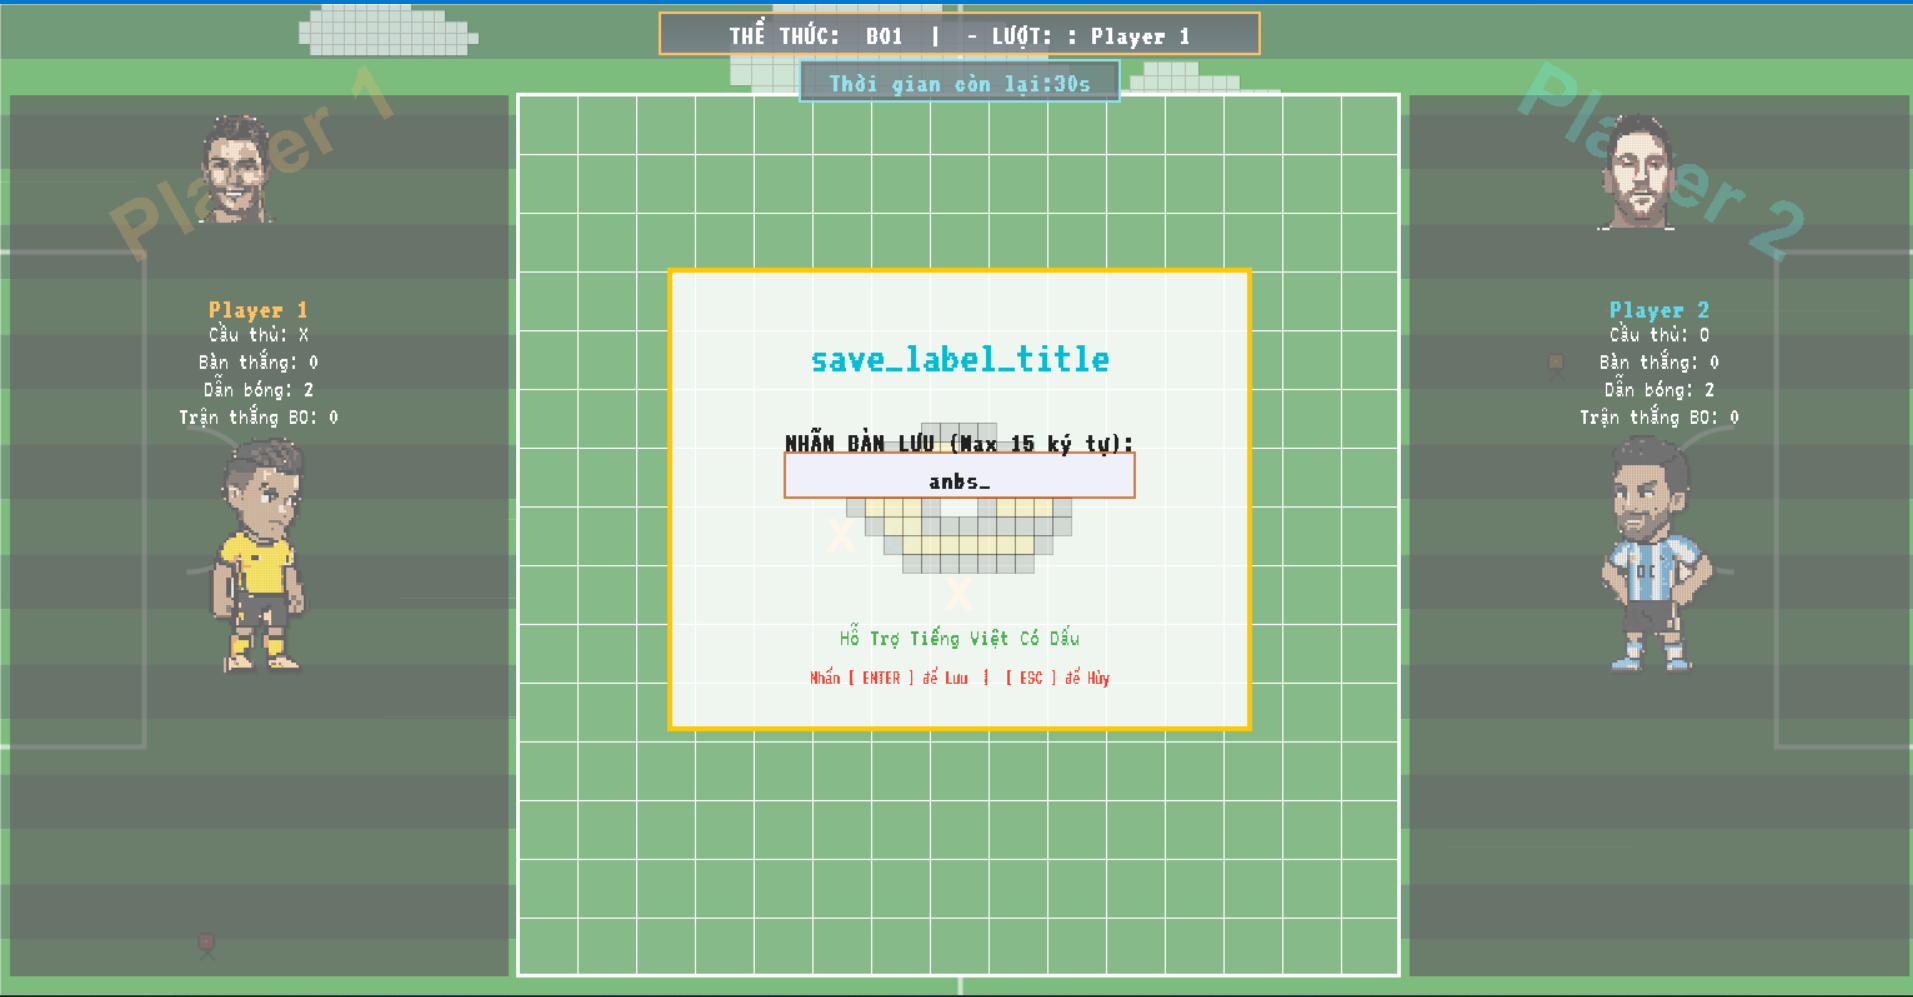
\includegraphics[width=0.45\linewidth]{images/ch4_save_game_2.png}
\caption*{Hình 4.12: Hình minh họa SaveGameScreen}
\end{figure}

\captionsetup{type=lstlisting}
\renewcommand{\arraystretch}{0.8}
\captionof{lstlisting}{Mã nguồn RenderSaveGameScreen: bố cục và banner}\label{lst:ch4_save_render}
\begin{longtable}{|>{\ttfamily\small\color{black}\raggedleft\arraybackslash}p{0.8cm}|>{\ttfamily\small\color{black}\arraybackslash}p{0.85\linewidth}|}
\hline
\normalfont\bfseries STT & \normalfont\bfseries Mã nguồn \\ \hline
1 & \cppkw{void} RenderSaveGameScreen(\cpptype{HDC} hdc, \cppkw{int} selectedOption, \cppkw{const} \cpptype{std::wstring} \&statusMessage, \cppkw{int} screenWidth, \cppkw{int} screenHeight) \\ \hline
2 & \{ \\ \hline
3 & \ \ Gdiplus::Graphics g(hdc); \\ \hline
4 & \ \ DrawProceduralStadium(g, screenWidth, screenHeight); \\ \hline
5 & \ \ \cppkw{int} panelW = UIScaler::SX(900); \\ \hline
6 & \ \ \cppkw{int} panelH = UIScaler::SY(540); \\ \hline
7 & \ \ \cppkw{int} panelX = (screenWidth - panelW) / 2; \\ \hline
8 & \ \ \cppkw{int} panelY = (screenHeight - panelH) / 2; \\ \hline
9 & \ \ Gdiplus::SolidBrush bgBrush(ToGdiColor(Theme::GlassWhite)); \\ \hline
10 & \ \ g.FillRectangle(\&bgBrush, panelX, panelY, panelW, panelH); \\ \hline
11 & \ \ DrawPixelBanner(g, hdc, GetText("save\_title").c\_str(), screenWidth / 2, panelY + UIScaler::SY(45), panelW - UIScaler::SX(40), ToCOLORREF(Palette::White), RGB(0, 150, 255), "Asset/models/bg/cassette.txt"); \\ \hline
12 & \} \\ \hline
\end{longtable}

\subsection*{4.6.10. SummaryScreen}
\addcontentsline{toc}{subsection}{\textcolor{black}{4.6.10. SummaryScreen}}

\setlength{\parindent}{1.5em} SummaryScreen là màn hình tổng kết sau ván/series, tập trung hiển thị thông tin cốt lõi: người thắng, tỷ số, thời gian, và các nút hành động (chơi lại, về menu). UI dùng banner màu nổi và hiệu ứng glow theo màu người thắng để nhấn mạnh kết quả.

\setlength{\parindent}{1.5em} Các màu victory banner và highlight kết quả lấy theo Theme (\texttt{P1TurnBorder} hoặc \texttt{P2TurnBorder}), nên người chơi nhận biết nhanh bên thắng mà không cần đọc chữ.

\setlength{\parindent}{1.5em} Phần số liệu được căn giữa theo chiều dọc, dùng font lớn để đảm bảo đọc nhanh. Các nút điều hướng được bố trí dưới cùng và tách biệt bằng khoảng đệm lớn để tránh bấm nhầm.

\begin{table}[H]
\caption*{Hình 4.13: Hình minh họa SummaryScreen}
\addcontentsline{lof}{figure}{Hình 4.13: Hình minh họa SummaryScreen}
\centering
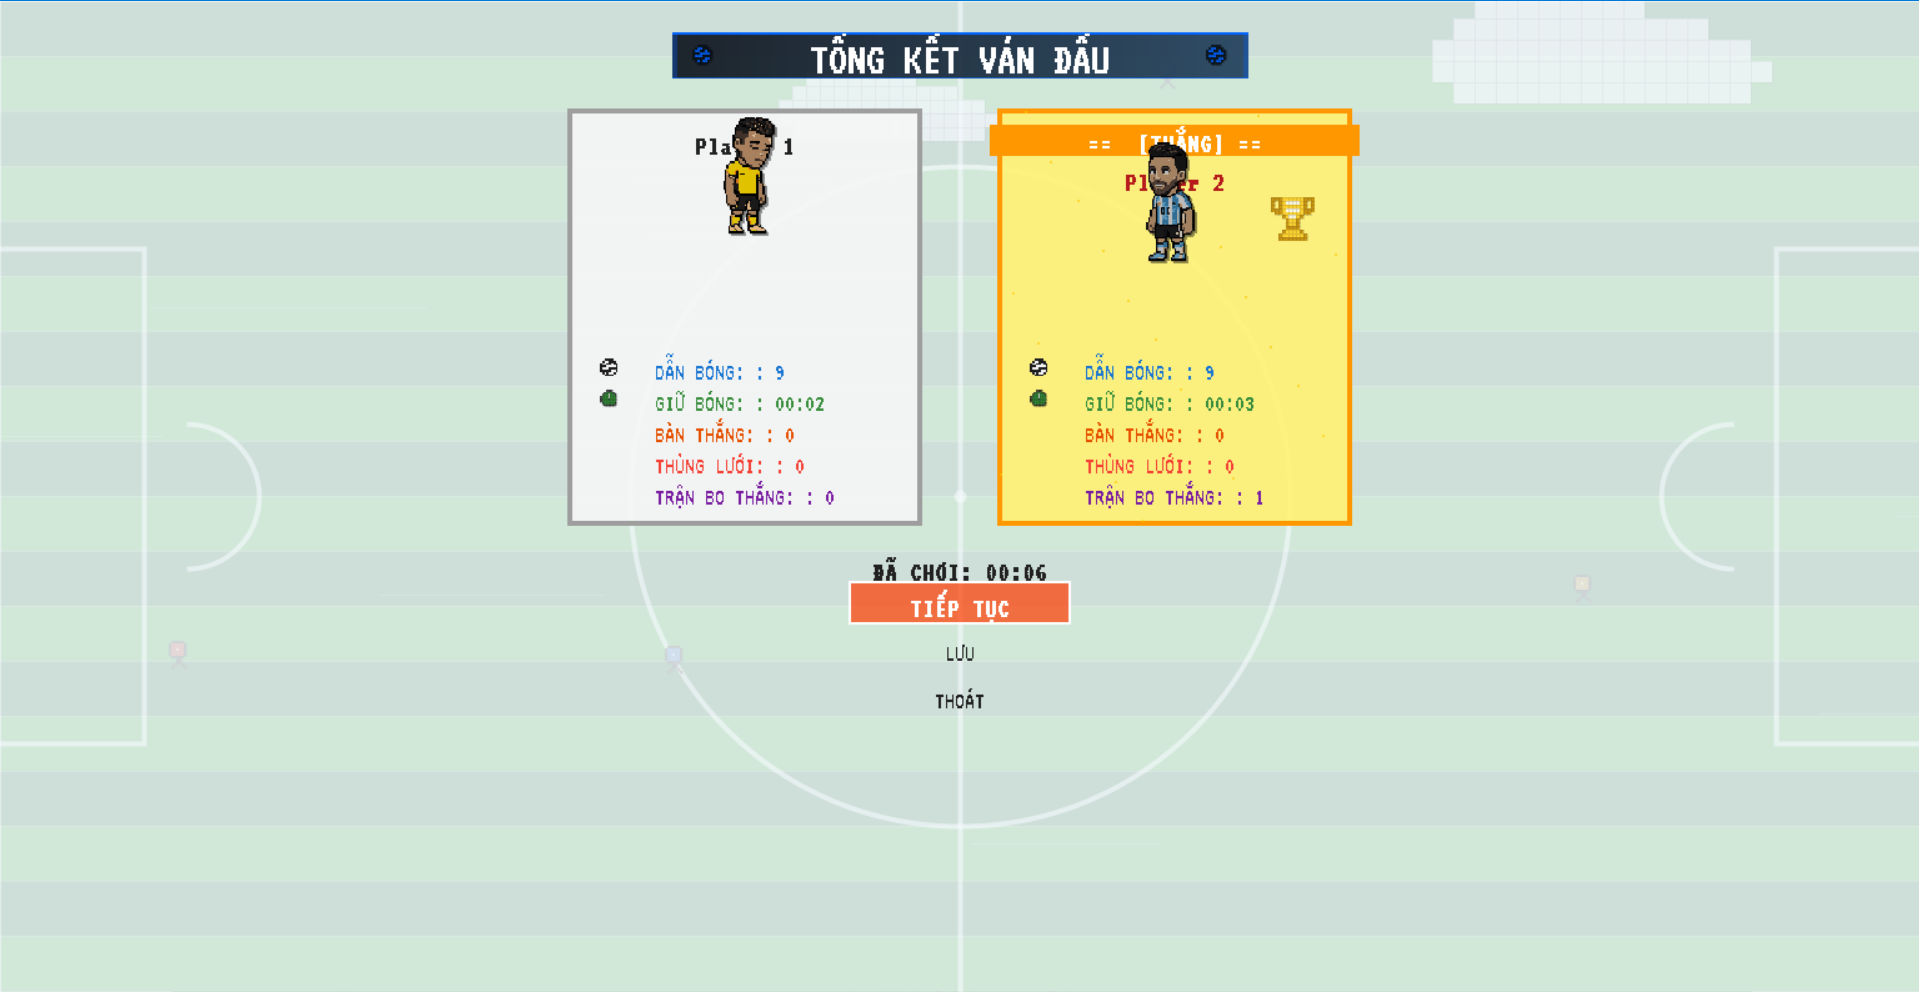
\includegraphics[width=0.9\linewidth]{images/ch4_summary.png}
\end{table}

\captionsetup{type=lstlisting}
\renewcommand{\arraystretch}{0.8}
\captionof{lstlisting}{Mã nguồn RenderSummaryScreen: banner và vùng kết quả}\label{lst:ch4_summary_render}
\begin{longtable}{|>{\ttfamily\small\color{black}\raggedleft\arraybackslash}p{0.8cm}|>{\ttfamily\small\color{black}\arraybackslash}p{0.85\linewidth}|}
\hline
\normalfont\bfseries STT & \normalfont\bfseries Mã nguồn \\ \hline
1 & \cppkw{void} RenderSummaryScreen(\cpptype{HDC} hdc, \cppkw{const} \cpptype{PlayState} *state, \cppkw{int} screenWidth, \cppkw{int} screenHeight) \\ \hline
2 & \{ \\ \hline
3 & \ \ Gdiplus::Graphics g(hdc); \\ \hline
4 & \ \ DrawProceduralStadium(g, screenWidth, screenHeight); \\ \hline
5 & \ \ \cppkw{int} panelW = UIScaler::SX(800); \\ \hline
6 & \ \ \cppkw{int} panelH = UIScaler::SY(420); \\ \hline
7 & \ \ \cppkw{int} panelX = (screenWidth - panelW) / 2; \\ \hline
8 & \ \ \cppkw{int} panelY = (screenHeight - panelH) / 2; \\ \hline
9 & \ \ Gdiplus::SolidBrush bgBrush(ToGdiColor(Theme::GlassWhite)); \\ \hline
10 & \ \ g.FillRectangle(\&bgBrush, panelX, panelY, panelW, panelH); \\ \hline
11 & \ \ DrawPixelBanner(g, hdc, GetText("summary\_title").c\_str(), screenWidth / 2, panelY + UIScaler::SY(45), panelW - UIScaler::SX(40), ToCOLORREF(Palette::White), RGB(255, 180, 0), "Asset/models/bg/trophy.txt"); \\ \hline
12 & \} \\ \hline
\end{longtable}

\section*{4.7. Tối ưu hóa và quản lý tài nguyên}
\addcontentsline{toc}{section}{\textcolor{black}{4.7. Tối ưu hóa và quản lý tài nguyên}}

\setlength{\parindent}{1.5em} Hệ thống có cơ chế dọn cache tập trung để tránh rò rỉ bộ nhớ. Hàm \texttt{ClearUICaches} giải phóng toàn bộ bitmap cache và brush cache khi cần (ví dụ khi đổi độ phân giải lớn hoặc thoát game).

\setlength{\parindent}{1.5em} Hàm này dọn tuần tự từng nhóm cache (model, avatar, football, trophy, clock, action, brush). Việc dọn theo nhóm giúp tránh bỏ sót và đảm bảo bộ nhớ đồ họa không bị giữ lại sau khi đổi scene lớn hoặc khi tắt game.

\captionsetup{type=lstlisting}
\renewcommand{\arraystretch}{0.8}
\captionof{lstlisting}{Mã nguồn Dọn cache UI tập trung}\label{lst:ch4_clear_caches}
\begin{longtable}{|>{\ttfamily\small\color{black}\raggedleft\arraybackslash}p{0.8cm}|>{\ttfamily\small\color{black}\arraybackslash}p{0.85\linewidth}|}
\hline
\normalfont\bfseries STT & \normalfont\bfseries Mã nguồn \\ \hline
1 & \cppkw{void} ClearUICaches() \\ \hline
2 & \{ \\ \hline
3 & \ \ \cppkw{for} (\cppkw{auto} \&pair : g\_ModelCache) \{ \cppkw{if} (pair.second) \cppkw{delete} pair.second; \} \\ \hline
4 & \ \ g\_ModelCache.clear(); \\ \hline
5 &  \\ \hline
6 & \ \ \cppkw{for} (\cppkw{auto} \&pair : g\_AvatarCache) \{ \cppkw{if} (pair.second) \cppkw{delete} pair.second; \} \\ \hline
7 & \ \ g\_AvatarCache.clear(); \\ \hline
8 &  \\ \hline
9 & \ \ \cppkw{for} (\cppkw{auto} \&pair : g\_BrushCache) \{ \cppkw{if} (pair.second) \cppkw{delete} pair.second; \} \\ \hline
10 & \ \ g\_BrushCache.clear(); \\ \hline
11 & \} \\ \hline
\end{longtable}

\setlength{\parindent}{1.5em} Ngoài ra, mô hình ``data-driven pixel art'' giúp giảm kích thước asset ảnh, đồng thời cho phép thay đổi palette nhanh theo theme mà không cần sửa lại sprite.

\section*{4.8. Vòng lặp ứng dụng và điều phối input}
\addcontentsline{toc}{section}{\textcolor{black}{4.8. Vòng lặp ứng dụng và điều phối input}}

\setlength{\parindent}{1.5em} Phần này mô tả vòng lặp chính của ứng dụng (message pump + update/render) và cơ chế throttling input để tránh spam phím. Hai cơ chế này quyết định tính ổn định FPS và cảm giác điều khiển trong UI.

\subsection*{4.8.1. Message pump, dt và giới hạn bước nhảy thời gian}
\addcontentsline{toc}{subsection}{\textcolor{black}{4.8.1. Message pump, dt và giới hạn bước nhảy thời gian}}

\setlength{\parindent}{1.5em} Vòng lặp chính xử lý toàn bộ tin nhắn đang chờ, sau đó mới chạy update và render. Thời gian khung hình \texttt{dt} được tính từ \texttt{high\_resolution\_clock} và bị chặn ở ngưỡng 0.1s để tránh "nhảy vọt" khi người dùng kéo/di chuyển cửa sổ. Điều này giữ logic ổn định và tránh cập nhật quá lớn gây vỡ animation.

\captionsetup{type=lstlisting}
\renewcommand{\arraystretch}{0.8}
\captionof{lstlisting}{Vòng lặp chính: xử lý message và giới hạn dt}\label{lst:ch4_main_loop}
\begin{longtable}{|>{\ttfamily\small\color{black}\raggedleft\arraybackslash}p{0.8cm}|>{\ttfamily\small\color{black}\arraybackslash}p{0.85\linewidth}|}
\hline
\normalfont\bfseries STT & \normalfont\bfseries Mã nguồn \\ \hline
1 & \cppkw{while} (bRunning) \{ \\ \hline
2 & \ \ \cppkw{while} (PeekMessage(\&msg, NULL, 0, 0, PM\_REMOVE)) \{ \\ \hline
3 & \ \ \ \ \cppkw{if} (msg.message == WM\_QUIT) \{ bRunning = \cppkw{false}; \cppkw{break}; \} \\ \hline
4 & \ \ \ \ TranslateMessage(\&msg); \ DispatchMessage(\&msg); \\ \hline
5 & \ \ \} \\ \hline
6 & \ \ \cppkw{if} (!bRunning) \cppkw{break}; \\ \hline
7 & \ \ \cppkw{auto} frameStart = std::chrono::high\_resolution\_clock::now(); \\ \hline
8 & \ \ std::chrono::duration<double> elapsed = frameStart - lastTime; \\ \hline
9 & \ \ lastTime = frameStart; \\ \hline
10 & \ \ \cppkw{double} dt = elapsed.count(); \\ \hline
11 & \ \ \cppkw{if} (dt > 0.1) dt = 0.1; \\ \hline
12 & \ \ g\_GlobalAnimTime += (float)dt; \\ \hline
13 & \} \\ \hline
\end{longtable}

\subsection*{4.8.2. Throttling input và chống autorepeat quá nhanh}
\addcontentsline{toc}{subsection}{\textcolor{black}{4.8.2. Throttling input và chống autorepeat quá nhanh}}

\setlength{\parindent}{1.5em} Ở menu và các màn hình điều hướng, phím di chuyển được giới hạn tốc độ để tránh "nhảy" nhiều mục khi người dùng giữ phím. Hệ thống tách nhấn thường và autorepeat, áp dụng ngưỡng 80ms cho nhấn tay và 150ms cho phím giữ. Cách này giữ cảm giác điều khiển mượt và dễ kiểm soát.

\captionsetup{type=lstlisting}
\renewcommand{\arraystretch}{0.8}
\captionof{lstlisting}{Throttling phím điều hướng trong MenuScreen}\label{lst:ch4_menu_throttle}
\begin{longtable}{|>{\ttfamily\small\color{black}\raggedleft\arraybackslash}p{0.8cm}|>{\ttfamily\small\color{black}\arraybackslash}p{0.85\linewidth}|}
\hline
\normalfont\bfseries STT & \normalfont\bfseries Mã nguồn \\ \hline
1 & \cppkw{bool} isRepeat = (wParam \& 0x20000) != 0; \\ \hline
2 & WPARAM rawKey = wParam \& 0xFFFF; \\ \hline
3 & \cppkw{static} ULONGLONG lastMoveTime = 0; \\ \hline
4 & ULONGLONG now = GetTickCount64(); \\ \hline
5 & \cppkw{bool} canMove = (now - lastMoveTime > (ULONGLONG)(isRepeat ? 150 : 80)); \\ \hline
6 & \cppkw{if} (rawKey == 'W' || rawKey == 'w' || rawKey == VK\_UP) \{ \\ \hline
7 & \ \ \cppkw{if} (!canMove) \cppkw{return} \cppkw{false}; \\ \hline
8 & \ \ selectedOption--; \\ \hline
9 & \ \ \cppkw{if} (!isRepeat) PlaySFX("sfx\_move"); \\ \hline
10 & \ \ lastMoveTime = now; \\ \hline
11 & \} \\ \hline
\end{longtable}

\newpage
\chapter*{\centering{\MakeUppercase{CHƯƠNG 5. LUẬT CHƠI VÀ CƠ CHẾ KIỂM TRA}}}
\addcontentsline{toc}{chapter}{\textcolor{fitblue}{\MakeUppercase{CHƯƠNG 5. LUẬT CHƠI VÀ CƠ CHẾ KIỂM TRA}}}
\setlength{\parindent}{1.5em}

\section*{5.1. Luật và biến thể}
\addcontentsline{toc}{section}{\textcolor{black}{5.1. Luật và biến thể}}

\setlength{\parindent}{1.5em} Chương này tập trung mô tả hệ luật của trò chơi, cách kiểm tra hợp lệ của nước đi và cơ chế phán xét kết quả theo thời gian thực. Toàn bộ logic luật chơi nằm trong mô-đun GameRules và GameEngine, trong khi trạng thái được lưu ở PlayState. Thiết kế tách lớp giúp luật chơi độc lập với UI, đảm bảo có thể tái sử dụng cho nhiều chế độ và kích thước bàn cờ.

\subsection*{5.1.1. Caro 5 quân và Tic-Tac-Toe}
\addcontentsline{toc}{subsection}{\textcolor{black}{5.1.1. Caro 5 quân và Tic-Tac-Toe}}

\setlength{\parindent}{1.5em} Dự án hỗ trợ hai chế độ chơi được định nghĩa bằng PlayMode: MODE\_CARO (Gomoku/Caro 5 quân) và MODE\_TTT (Tic-Tac-Toe 3 quân). Hai chế độ dùng chung một engine, chỉ khác tham số độ dài chuỗi thắng (winLength). Nhờ đó, quy tắc thắng được thay đổi mà không cần nhân đôi code.

\captionsetup{type=lstlisting}
\renewcommand{\arraystretch}{0.8}
\captionof{lstlisting}{Xác định độ dài chuỗi thắng theo chế độ chơi}\label{lst:ch5_win_length}
\begin{longtable}{|>{\ttfamily\small\color{black}\raggedleft\arraybackslash}p{0.8cm}|>{\ttfamily\small\color{black}\arraybackslash}p{0.85\linewidth}|}
\hline
\normalfont\bfseries STT & \normalfont\bfseries Mã nguồn \\ \hline
1 & \cppkw{const} \cppkw{int} winLength = (state->gameMode == MODE\_CARO) ? 5 : 3; \\ \hline
\end{longtable}

\setlength{\parindent}{1.5em} Bàn cờ lưu trong ma trận hai chiều \texttt{board[MAX\_BOARD\_SIZE][MAX\_BOARD\_SIZE]} với kích thước thực tế theo \texttt{boardSize}. Mỗi ô có giá trị \texttt{CELL\_EMPTY}, \texttt{CELL\_PLAYER1} hoặc \texttt{CELL\_PLAYER2}, cho phép thuật toán kiểm tra thắng hoạt động nhất quán trên mọi kích thước. Ở chế độ Caro, giá trị mặc định là 15x15; trong khi Tic-Tac-Toe thường dùng 3x3, nhưng thuật toán vẫn giữ nguyên logic.

\subsection*{5.1.2. Kiểm tra hợp lệ và biên}
\addcontentsline{toc}{subsection}{\textcolor{black}{5.1.2. Kiểm tra hợp lệ và biên}}

\setlength{\parindent}{1.5em} Trước khi đặt quân, hệ thống bắt buộc kiểm tra hai điều kiện: (1) tọa độ nằm trong phạm vi bàn cờ, (2) ô đang trống. Việc kiểm tra biên không dùng hằng số cứng mà dựa vào \texttt{boardSize}, giúp luật chơi tự thích nghi khi người chơi thay đổi kích thước bàn cờ.

\captionsetup{type=lstlisting}
\renewcommand{\arraystretch}{0.8}
\captionof{lstlisting}{Mã nguồn kiểm tra hợp lệ nước đi}\label{lst:ch5_valid_move}
\begin{longtable}{|>{\ttfamily\small\color{black}\raggedleft\arraybackslash}p{0.8cm}|>{\ttfamily\small\color{black}\arraybackslash}p{0.85\linewidth}|}
\hline
\normalfont\bfseries STT & \normalfont\bfseries Mã nguồn \\ \hline
1 & \cppkw{bool} isValidMove(\cppkw{const} PlayState* state, \cppkw{int} row, \cppkw{int} col) \{ \\ \hline
2 & \ \ \cppkw{if} (row < 0 || row >= state->boardSize || col < 0 || col >= state->boardSize) \\ \hline
3 & \ \ \ \ \cppkw{return} \cppkw{false}; \\ \hline
4 & \ \ \cppkw{return} state->board[row][col] == CELL\_EMPTY; \\ \hline
5 & \} \\ \hline
\end{longtable}

\setlength{\parindent}{1.5em} Thiết kế này đảm bảo không thể đánh tràn biên, đồng thời tránh ghi đè quân đã có. Đây là tầng bảo vệ đầu tiên trước khi engine chấp nhận cập nhật trạng thái trận đấu.

\subsection*{5.1.3. Trạng thái tối thiểu phục vụ kiểm tra}
\addcontentsline{toc}{subsection}{\textcolor{black}{5.1.3. Trạng thái tối thiểu phục vụ kiểm tra}}

\setlength{\parindent}{1.5em} Để việc kiểm tra thắng và kết thúc ván diễn ra chính xác, PlayState duy trì các trường dữ liệu tối thiểu: kích thước bàn cờ, ma trận trạng thái, nước đi cuối, danh sách ô thắng và bộ đếm số nước đi của mỗi người chơi. Những trường này giúp thuật toán kiểm tra thắng và điều kiện hòa chạy nhanh mà không phải quét lại toàn bộ bàn cờ.

\captionsetup{type=lstlisting}
\renewcommand{\arraystretch}{0.8}
\captionof{lstlisting}{Các trường dữ liệu phục vụ kiểm tra thắng và hòa}\label{lst:ch5_playstate_core}
\begin{longtable}{|>{\ttfamily\small\color{black}\raggedleft\arraybackslash}p{0.8cm}|>{\ttfamily\small\color{black}\arraybackslash}p{0.85\linewidth}|}
\hline
\normalfont\bfseries STT & \normalfont\bfseries Mã nguồn \\ \hline
1 & \cppkw{int} boardSize = 15; \\ \hline
2 & \cppkw{int} board[MAX\_BOARD\_SIZE][MAX\_BOARD\_SIZE] = \{0\}; \\ \hline
3 & \cppkw{int} lastMoveRow = -1; \\ \hline
4 & \cppkw{int} lastMoveCol = -1; \\ \hline
5 & std::vector<std::pair<int, int>> winningCells; \\ \hline
6 & \cppkw{int} movesCount; \ \textcolor{dkgreen}{// nằm trong PlayerInfo2 của từng người chơi} \\ \hline
\end{longtable}

\section*{5.2. Thuật toán xác định thắng}
\addcontentsline{toc}{section}{\textcolor{black}{5.2. Thuật toán xác định thắng}}

\subsection*{5.2.1. Quét 4 hướng tối ưu}
\addcontentsline{toc}{subsection}{\textcolor{black}{5.2.1. Quét 4 hướng tối ưu}}

\setlength{\parindent}{1.5em} Thuật toán phán xét thắng sử dụng ô vừa đặt làm điểm neo và quét theo bốn hướng cơ bản: ngang, dọc, chéo chính và chéo phụ. Mỗi hướng được quét hai chiều (tiến và lùi) để gom toàn bộ chuỗi liên tiếp cùng màu. Nhờ chỉ quét từ nước đi cuối, chi phí tính toán gần như tuyến tính theo độ dài chuỗi thắng thay vì theo kích thước bàn cờ, và dừng sớm ngay khi phát hiện thắng.

\captionsetup{type=lstlisting}
\renewcommand{\arraystretch}{0.8}
\captionof{lstlisting}{Mã nguồn quét 4 hướng từ nước đi cuối}\label{lst:ch5_scan_four_dirs}
\begin{longtable}{|>{\ttfamily\small\color{black}\raggedleft\arraybackslash}p{0.8cm}|>{\ttfamily\small\color{black}\arraybackslash}p{0.85\linewidth}|}
\hline
\normalfont\bfseries STT & \normalfont\bfseries Mã nguồn \\ \hline
1 & \cppkw{static} \cppkw{const} \cppkw{int} dr[] = \{ 0, 1, 1, \ 1 \}; \\ \hline
2 & \cppkw{static} \cppkw{const} \cppkw{int} dc[] = \{ 1, 0, 1, -1 \}; \\ \hline
3 & \cppkw{for} (\cppkw{int} dir = 0; dir < 4; dir++) \{ \\ \hline
4 & \ \ std::vector<std::pair<int, int>> line; \\ \hline
5 & \ \ line.push\_back(\{ lastRow, lastCol \}); \\ \hline
6 & \ \ \textcolor{dkgreen}{// Quét tiến} \\ \hline
7 & \ \ \cppkw{for} (\cppkw{int} step = 1; step < size; step++) \{ \ldots \} \\ \hline
8 & \ \ \textcolor{dkgreen}{// Quét lùi} \\ \hline
9 & \ \ \cppkw{for} (\cppkw{int} step = 1; step < size; step++) \{ \ldots \} \\ \hline
10 & \ \ \cppkw{if} ((\cppkw{int})line.size() >= winLength) \{ \ldots \} \\ \hline
11 & \} \\ \hline
\end{longtable}

\setlength{\parindent}{1.5em} Thuật toán dừng ngay khi phát hiện chuỗi đủ dài. Điều này giảm độ trễ khi bàn cờ lớn và đảm bảo việc kiểm tra thắng vẫn mượt trong thời gian thực.

\subsection*{5.2.3. Kiểm tra điều kiện hợp lệ trước khi quét}
\addcontentsline{toc}{subsection}{\textcolor{black}{5.2.3. Kiểm tra điều kiện hợp lệ trước khi quét}}

\setlength{\parindent}{1.5em} Trước khi bắt đầu quét, hệ thống xác thực nước đi cuối có nằm trong biên và có quân thực sự hay không. Điều này tránh các phép quét thừa và ngăn lỗi khi trạng thái chưa được khởi tạo đầy đủ (ví dụ lúc vừa reset bàn hoặc chưa có nước đi).

\captionsetup{type=lstlisting}
\renewcommand{\arraystretch}{0.8}
\captionof{lstlisting}{Chặn sớm khi nước đi cuối không hợp lệ}\label{lst:ch5_early_abort}
\begin{longtable}{|>{\ttfamily\small\color{black}\raggedleft\arraybackslash}p{0.8cm}|>{\ttfamily\small\color{black}\arraybackslash}p{0.85\linewidth}|}
\hline
\normalfont\bfseries STT & \normalfont\bfseries Mã nguồn \\ \hline
1 & \cppkw{if} (lastRow < 0 || lastRow >= size || lastCol < 0 || lastCol >= size) \\ \hline
2 & \ \ \cppkw{return} -1; \\ \hline
3 & \cppkw{const} \cppkw{int} currentPiece = state->board[lastRow][lastCol]; \\ \hline
4 & \cppkw{if} (currentPiece == CELL\_EMPTY) \\ \hline
5 & \ \ \cppkw{return} -1; \\ \hline
\end{longtable}

\subsection*{5.2.2. Truy vết winningCells cho highlight}
\addcontentsline{toc}{subsection}{\textcolor{black}{5.2.2. Truy vết winningCells cho highlight}}

\setlength{\parindent}{1.5em} Hàm \texttt{checkWinCondition()} hỗ trợ tham số tùy chọn \texttt{outWinCells}. Khi phát hiện thắng, toàn bộ chuỗi liên tiếp được trả về, không bị cắt ở đúng \texttt{winLength}. Điều này xử lý đúng trường hợp người chơi đặt quân ở giữa, nối hai đoạn rời thành một chuỗi dài hơn. Danh sách ô thắng được lưu trong PlayState và dùng trực tiếp bởi lớp render để highlight.

\captionsetup{type=lstlisting}
\renewcommand{\arraystretch}{0.8}
\captionof{lstlisting}{Trả về toàn bộ chuỗi thắng và lưu trong PlayState}\label{lst:ch5_win_cells}
\begin{longtable}{|>{\ttfamily\small\color{black}\raggedleft\arraybackslash}p{0.8cm}|>{\ttfamily\small\color{black}\arraybackslash}p{0.85\linewidth}|}
\hline
\normalfont\bfseries STT & \normalfont\bfseries Mã nguồn \\ \hline
1 & \cppkw{if} ((\cppkw{int})line.size() >= winLength) \{ \\ \hline
2 & \ \ \cppkw{if} (outWinCells) *outWinCells = line; \\ \hline
3 & \ \ \cppkw{return} currentPiece; \\ \hline
4 & \} \\ \hline
\end{longtable}

\setlength{\parindent}{1.5em} Khi vẽ bàn cờ, UIComponents sử dụng danh sách này để tạo hiệu ứng highlight động trên đúng các ô thắng, đảm bảo trực quan và nhất quán với luật chơi.

\captionsetup{type=lstlisting}
\renewcommand{\arraystretch}{0.8}
\captionof{lstlisting}{Highlight các ô thắng dựa trên winningCells}\label{lst:ch5_ui_highlight}
\begin{longtable}{|>{\ttfamily\small\color{black}\raggedleft\arraybackslash}p{0.8cm}|>{\ttfamily\small\color{black}\arraybackslash}p{0.85\linewidth}|}
\hline
\normalfont\bfseries STT & \normalfont\bfseries Mã nguồn \\ \hline
1 & \cppkw{if} (!state->winningCells.empty()) \{ \\ \hline
2 & \ \ \cppkw{for} (\cppkw{const} \cppkw{auto} \&wCell : state->winningCells) \{ \\ \hline
3 & \ \ \ \ \cppkw{int} drawX = offsetX + wCell.second * cellSize; \\ \hline
4 & \ \ \ \ \cppkw{int} drawY = offsetY + wCell.first * cellSize; \\ \hline
5 & \ \ \ \ g.FillRectangle(winBrush, drawX + 1, drawY + 1, cellSize - 2, cellSize - 2); \\ \hline
6 & \ \ \ \ g.DrawRectangle(\&winPen, drawX + 2, drawY + 2, cellSize - 4, cellSize - 4); \\ \hline
7 & \ \ \} \\ \hline
8 & \} \\ \hline
\end{longtable}

\section*{5.3. Trạng thái kết thúc đặc biệt}
\addcontentsline{toc}{section}{\textcolor{black}{5.3. Trạng thái kết thúc đặc biệt}}

\subsection*{5.3.1. Hòa và chặn nước đi}
\addcontentsline{toc}{subsection}{\textcolor{black}{5.3.1. Hòa và chặn nước đi}}

\setlength{\parindent}{1.5em} Ván đấu kết thúc hòa nếu toàn bộ bàn cờ đã đầy mà không xuất hiện chuỗi thắng. Thay vì quét lại toàn bộ bàn cờ để kiểm tra còn ô trống hay không, hệ thống dùng tổng số nước đi của hai người chơi, giúp tối ưu thời gian kiểm tra.

\captionsetup{type=lstlisting}
\renewcommand{\arraystretch}{0.8}
\captionof{lstlisting}{Kiểm tra điều kiện hòa bằng bộ đếm nước đi}\label{lst:ch5_draw_check}
\begin{longtable}{|>{\ttfamily\small\color{black}\raggedleft\arraybackslash}p{0.8cm}|>{\ttfamily\small\color{black}\arraybackslash}p{0.85\linewidth}|}
\hline
\normalfont\bfseries STT & \normalfont\bfseries Mã nguồn \\ \hline
1 & \cppkw{if} (state->p1.movesCount + state->p2.movesCount == size * size) \\ \hline
2 & \ \ \cppkw{return} CELL\_EMPTY; \\ \hline
3 & \cppkw{return} -1; \\ \hline
\end{longtable}

\setlength{\parindent}{1.5em} Khi \texttt{checkWinCondition()} trả về trạng thái thắng hoặc hòa, GameEngine lập tức kết thúc ván đấu, cập nhật trạng thái và người thắng trong PlayState.

\captionsetup{type=lstlisting}
\renewcommand{\arraystretch}{0.8}
\captionof{lstlisting}{Cập nhật trạng thái ván đấu sau khi kiểm tra thắng}\label{lst:ch5_process_move}
\begin{longtable}{|>{\ttfamily\small\color{black}\raggedleft\arraybackslash}p{0.8cm}|>{\ttfamily\small\color{black}\arraybackslash}p{0.85\linewidth}|}
\hline
\normalfont\bfseries STT & \normalfont\bfseries Mã nguồn \\ \hline
1 & \cppkw{int} winStatus = checkWinCondition(state, row, col, \&state->winningCells); \\ \hline
2 & \cppkw{if} (winStatus != -1) \{ \\ \hline
3 & \ \ state->status = MATCH\_FINISHED; \\ \hline
4 & \ \ state->winner = winStatus; \\ \hline
5 & \} \cppkw{else} \{ \ \ switchTurn(state); \} \\ \hline
\end{longtable}

\subsection*{5.3.2. Cơ chế BO (Best-of) và thắng series}
\addcontentsline{toc}{subsection}{\textcolor{black}{5.3.2. Cơ chế BO (Best-of) và thắng series}}

\setlength{\parindent}{1.5em} Ngoài luật thắng từng ván, hệ thống còn hỗ trợ luật thắng theo series BO (BO1/BO3/BO5) thông qua \texttt{targetScore}. Sau mỗi ván thắng, engine kiểm tra số bàn thắng cần để kết thúc series. Nếu đã đủ, \texttt{matchWins} được tăng, và \texttt{totalWins} được reset để bắt đầu series tiếp theo.

\captionsetup{type=lstlisting}
\renewcommand{\arraystretch}{0.8}
\captionof{lstlisting}{Xác định thắng series BO trong processMove}\label{lst:ch5_bo_series}
\begin{longtable}{|>{\ttfamily\small\color{black}\raggedleft\arraybackslash}p{0.8cm}|>{\ttfamily\small\color{black}\arraybackslash}p{0.85\linewidth}|}
\hline
\normalfont\bfseries STT & \normalfont\bfseries Mã nguồn \\ \hline
1 & \cppkw{int} winRequired = (state->targetScore + 1) / 2; \\ \hline
2 & \cppkw{if} (state->targetScore > 1) \{ \ \ winRequired = state->targetScore; \} \\ \hline
3 & \cppkw{bool} seriesWon = (state->p1.totalWins >= winRequired || state->p2.totalWins >= winRequired); \\ \hline
4 & \cppkw{if} (seriesWon) \{ \ldots \} \\ \hline
\end{longtable}

\setlength{\parindent}{1.5em} Cách tính \texttt{winRequired} đảm bảo BO1 cần 1 ván, BO3 cần 2 ván, BO5 cần 3 ván. Với các thiết lập \texttt{targetScore} khác, hệ thống vẫn hoạt động nhất quán vì dùng \texttt{targetScore} làm mục tiêu trực tiếp.

\subsection*{5.3.3. Timeout và đồng bộ TimeSystem}
\addcontentsline{toc}{subsection}{\textcolor{black}{5.3.3. Timeout và đồng bộ TimeSystem}}

\setlength{\parindent}{1.5em} Hệ thống thời gian được tách riêng trong TimeSystem, sử dụng cơ chế tích lũy \texttt{dt} để đếm giây chính xác và tránh sai số khi khung hình không đều. Mỗi khi đủ một giây, \texttt{timeRemaining} giảm đi một đơn vị. Khi về 0, hệ thống báo timeout để xử lý đổi lượt.

\captionsetup{type=lstlisting}
\renewcommand{\arraystretch}{0.8}
\captionof{lstlisting}{Đếm ngược theo giây bằng bộ tích lũy thời gian}\label{lst:ch5_update_countdown}
\begin{longtable}{|>{\ttfamily\small\color{black}\raggedleft\arraybackslash}p{0.8cm}|>{\ttfamily\small\color{black}\arraybackslash}p{0.85\linewidth}|}
\hline
\normalfont\bfseries STT & \normalfont\bfseries Mã nguồn \\ \hline
1 & timeAccumulator += dt; \\ \hline
2 & \cppkw{if} (timeAccumulator >= 1.0) \{ \\ \hline
3 & \ \ timeAccumulator -= 1.0; \\ \hline
4 & \ \ state->timeRemaining--; \\ \hline
5 & \ \ \cppkw{if} (state->timeRemaining <= 0) \{ state->timeRemaining = 0; \} \\ \hline
6 & \ \ \cppkw{return} \cppkw{true}; \\ \hline
7 & \} \\ \hline
8 & \cppkw{return} \cppkw{false}; \\ \hline
\end{longtable}

\setlength{\parindent}{1.5em} PlayScreen đồng bộ timeout bằng cách lắng nghe cờ trả về từ \texttt{UpdateCountdown()}. Khi hết thời gian, hệ thống phát âm thanh timeout và đổi lượt ngay lập tức. Điều này biến thời gian thành một ràng buộc luật chơi trực tiếp, không chỉ là hiển thị giao diện.

\captionsetup{type=lstlisting}
\renewcommand{\arraystretch}{0.8}
\captionof{lstlisting}{Xử lý timeout và đổi lượt trong vòng lặp chơi}\label{lst:ch5_timeout_switch}
\begin{longtable}{|>{\ttfamily\small\color{black}\raggedleft\arraybackslash}p{0.8cm}|>{\ttfamily\small\color{black}\arraybackslash}p{0.85\linewidth}|}
\hline
\normalfont\bfseries STT & \normalfont\bfseries Mã nguồn \\ \hline
1 & \cppkw{if} (UpdateCountdown(state, dt)) \{ \\ \hline
2 & \ \ \cppkw{if} (state->timeRemaining <= 0) \{ \\ \hline
3 & \ \ \ \ PlaySFX("sfx\_timeout"); \\ \hline
4 & \ \ \ \ switchTurn(state); \\ \hline
5 & \ \ \} \\ \hline
6 & \} \\ \hline
\end{longtable}

\setlength{\parindent}{1.5em} Mỗi khi đổi lượt, \texttt{ResetTimer()} sẽ đọc \texttt{maxTurnTime} của người chơi hiện tại để thiết lập lại thời gian đếm ngược. Cách làm này hỗ trợ luật chơi bất đối xứng (hai người chơi có giới hạn thời gian khác nhau) và đảm bảo đồng bộ giữa luật chơi và hiển thị.

\newpage
\chapter*{\centering{\MakeUppercase{CHƯƠNG 6. BỘ MÁY ĐIỀU PHỐI TRẬN ĐẤU}}}
\addcontentsline{toc}{chapter}{\textcolor{fitblue}{\MakeUppercase{CHƯƠNG 6. BỘ MÁY ĐIỀU PHỐI TRẬN ĐẤU}}}
\setlength{\parindent}{1.5em}

\section*{6.1. Điều phối lượt đánh}
\addcontentsline{toc}{section}{\textcolor{black}{6.1. Điều phối lượt đánh}}

\setlength{\parindent}{1.5em} Bộ máy điều phối ván đấu được tập trung tại GameEngine. Mục tiêu của lớp này là đóng gói toàn bộ pipeline xử lý nước đi thành một điểm vào duy nhất, giúp UI (PlayScreen) chỉ phát lệnh hành động và nhận kết quả, không can thiệp trực tiếp vào luật. Cách tổ chức này tách rõ ba lớp trách nhiệm: GameRules phán xét, GameEngine điều phối, TimeSystem quản lý thời gian. Nhờ vậy, mọi cập nhật đều nhất quán, tránh sai lệch trạng thái khi có nhiều thao tác đồng thời (đặt quân, lưu lịch sử, cập nhật điểm, kiểm tra thắng, đổi lượt).

\subsection*{6.1.1. Luồng xử lý: Nhập lệnh \texorpdfstring{$\rightarrow$}{} Luật \texorpdfstring{$\rightarrow$}{} Cập nhật trạng thái}
\addcontentsline{toc}{subsection}{\textcolor{black}{6.1.1. Luồng xử lý: Nhập lệnh \texorpdfstring{$\rightarrow$}{} Luật \texorpdfstring{$\rightarrow$}{} Cập nhật trạng thái}}

\setlength{\parindent}{1.5em} Hàm \texttt{processMove()} là luồng chuẩn cho một nước đi: kiểm tra hợp lệ, ghi quân lên bàn, cập nhật nước đi cuối, lưu lịch sử, xóa redo (nếu có), cập nhật thống kê, sau đó kiểm tra thắng hoặc đổi lượt. Chỉ khi toàn bộ trạng thái đã cập nhật xong, hệ thống mới phát âm thanh hoặc chuyển màn hình. Thiết kế này giúp việc phục hồi (undo/redo) và đồng bộ thời gian không bị lệch, đồng thời tránh hiện tượng “bán cập nhật” khi có lỗi giữa chừng.

\setlength{\parindent}{1.5em} Để đảm bảo tính nguyên tử, các cập nhật quan trọng được thực hiện theo thứ tự cố định: (1) cập nhật bàn cờ và nước đi cuối, (2) ghi lịch sử và xóa redo, (3) cập nhật thống kê, (4) phán xét thắng/thua, (5) đổi lượt hoặc kết thúc ván. Thứ tự này phản ánh đúng logic vận hành của ván đấu và bảo toàn tính nhất quán khi undo/redo.

\captionsetup{type=lstlisting}
\renewcommand{\arraystretch}{0.8}
\captionof{lstlisting}{Luồng xử lý một nước đi trong processMove}\label{lst:ch6_process_move}
\begin{longtable}{|>{\ttfamily\small\color{black}\raggedleft\arraybackslash}p{0.8cm}|>{\ttfamily\small\color{black}\arraybackslash}p{0.85\linewidth}|}
\hline
\normalfont\bfseries STT & \normalfont\bfseries Mã nguồn \\ \hline
1 & \cppkw{if} (state->status != MATCH\_PLAYING || !isValidMove(state, row, col)) \\ \hline
2 & \ \ \cppkw{return} \cppkw{false}; \\ \hline
3 & state->board[row][col] = state->isP1Turn ? CELL\_PLAYER1 : CELL\_PLAYER2; \\ \hline
4 & state->lastMoveRow = row; \\ \hline
5 & state->lastMoveCol = col; \\ \hline
6 & state->matchHistory.push\_back(\{ row, col \}); \\ \hline
7 & state->redoStack.clear(); \\ \hline
8 & \cppkw{if} (state->isP1Turn) state->p1.movesCount++; \cppkw{else} state->p2.movesCount++; \\ \hline
9 & \cppkw{int} winStatus = checkWinCondition(state, row, col, \&state->winningCells); \\ \hline
10 & \cppkw{if} (winStatus != -1) \{ \\ \hline
11 & \ \ \cppkw{if} (winStatus == CELL\_PLAYER1) state->p1.totalWins++; \\ \hline
12 & \ \ \cppkw{else if} (winStatus == CELL\_PLAYER2) state->p2.totalWins++; \\ \hline
13 & \ \ \cppkw{int} winRequired = (state->targetScore + 1) / 2; \\ \hline
14 & \ \ \cppkw{if} (state->targetScore > 1) \{ winRequired = state->targetScore; \} \\ \hline
15 & \ \ \cppkw{bool} seriesWon = (state->p1.totalWins >= winRequired || state->p2.totalWins >= winRequired); \\ \hline
16 & \ \ \cppkw{if} (seriesWon) \{ \ldots \} \\ \hline
17 & \ \ state->status = MATCH\_FINISHED; \\ \hline
18 & \ \ state->winner = winStatus; \\ \hline
19 & \ \ PlaySFX("sfx\_whistle"); \ \ PlaySFX("sfx\_crowd"); \ \ PlaySFX("sfx\_siu"); \\ \hline
20 & \} \cppkw{else} \{ switchTurn(state); \} \\ \hline
\end{longtable}

\setlength{\parindent}{1.5em} Pipeline này đảm bảo nguyên tắc “nguồn sự thật duy nhất”: trạng thái luôn được cập nhật tập trung ở GameEngine, tránh sai lệch do cập nhật phân tán. Ngoài ra, việc lưu \texttt{lastMoveRow/Col} ngay tại thời điểm đặt quân giúp các bước kiểm tra thắng và highlight luôn bám đúng nước đi cuối.

\subsection*{6.1.2. Đồng bộ lượt và biến isP1Turn}
\addcontentsline{toc}{subsection}{\textcolor{black}{6.1.2. Đồng bộ lượt và biến isP1Turn}}

\setlength{\parindent}{1.5em} Biến \texttt{isP1Turn} trong PlayState đóng vai trò nguồn sự thật duy nhất cho lượt chơi. Mọi hệ thống phụ (UI, AI, TimeSystem) đều đọc biến này thay vì tự suy diễn. Hàm \texttt{switchTurn()} đảo lượt và reset thời gian theo cấu hình, đảm bảo đồng bộ tuyệt đối giữa luật chơi và bộ đếm giờ. Cơ chế này cũng giúp việc undo/redo khôi phục đúng lượt hiện tại mà không cần suy luận lại từ lịch sử.

\captionsetup{type=lstlisting}
\renewcommand{\arraystretch}{0.8}
\captionof{lstlisting}{Đổi lượt và đồng bộ timer}\label{lst:ch6_switch_turn}
\begin{longtable}{|>{\ttfamily\small\color{black}\raggedleft\arraybackslash}p{0.8cm}|>{\ttfamily\small\color{black}\arraybackslash}p{0.85\linewidth}|}
\hline
\normalfont\bfseries STT & \normalfont\bfseries Mã nguồn \\ \hline
1 & \cppkw{void} switchTurn(PlayState* state) \{ \\ \hline
2 & \ \ state->isP1Turn = !state->isP1Turn; \\ \hline
3 & \ \ state->timeRemaining = state->countdownTime; \\ \hline
4 & \ \ ResetTimer(state); \\ \hline
5 & \} \\ \hline
\end{longtable}

\section*{6.2. Điều phối match series}
\addcontentsline{toc}{section}{\textcolor{black}{6.2. Điều phối match series}}

\subsection*{6.2.1. BO1/BO3/BO5 và mục tiêu thắng}
\addcontentsline{toc}{subsection}{\textcolor{black}{6.2.1. BO1/BO3/BO5 và mục tiêu thắng}}

\setlength{\parindent}{1.5em} Quy tắc BO đã được trình bày ở chương luật chơi. Tại đây chỉ tập trung vào cách engine hiện thực hóa việc cộng dồn và chốt series. Sau mỗi ván thắng, GameEngine tăng \texttt{totalWins}, tính ngưỡng \texttt{winRequired} từ \texttt{targetScore} và kiểm tra đã đủ điều kiện thắng series hay chưa. Khi thắng series, \texttt{matchWins} tăng và \texttt{totalWins} được reset về 0 để chuẩn bị cho series tiếp theo. Việc tách biệt này giúp luật chơi rõ ràng, còn engine chỉ chịu trách nhiệm cập nhật trạng thái.

\captionsetup{type=lstlisting}
\renewcommand{\arraystretch}{0.8}
\captionof{lstlisting}{Xác định thắng series trong processMove}\label{lst:ch6_bo_series}
\begin{longtable}{|>{\ttfamily\small\color{black}\raggedleft\arraybackslash}p{0.8cm}|>{\ttfamily\small\color{black}\arraybackslash}p{0.85\linewidth}|}
\hline
\normalfont\bfseries STT & \normalfont\bfseries Mã nguồn \\ \hline
1 & \cppkw{int} winRequired = (state->targetScore + 1) / 2; \\ \hline
2 & \cppkw{if} (state->targetScore > 1) \{ winRequired = state->targetScore; \} \\ \hline
3 & \cppkw{bool} seriesWon = (state->p1.totalWins >= winRequired || state->p2.totalWins >= winRequired); \\ \hline
4 & \cppkw{if} (seriesWon) \{ \ldots \} \\ \hline
\end{longtable}

\setlength{\parindent}{1.5em} Cách tính này hoạt động nhất quán với mọi cấu hình \texttt{targetScore} và đảm bảo trạng thái series luôn đồng bộ với số ván đã thắng của từng người chơi.

\subsection*{6.2.2. Reset hiệp và bảo toàn tỷ số}
\addcontentsline{toc}{subsection}{\textcolor{black}{6.2.2. Reset hiệp và bảo toàn tỷ số}}

\setlength{\parindent}{1.5em} Khi chuyển sang một round mới trong cùng series, \texttt{startNextRound()} reset bàn cờ, lịch sử nước đi và dữ liệu thời gian, nhưng giữ nguyên điểm series. Điều này giúp kết quả từng ván tách biệt khỏi tiến trình series. Hệ thống cũng đưa con trỏ về giữa bàn và xóa danh sách ô thắng để bắt đầu ván mới sạch sẽ. Ngoài ra, bảng băm trạng thái (nếu dùng cho AI) được xóa để tránh dùng lại dữ liệu của ván trước.

\captionsetup{type=lstlisting}
\renewcommand{\arraystretch}{0.8}
\captionof{lstlisting}{Khởi tạo round mới, giữ nguyên tiến trình series}\label{lst:ch6_start_round}
\begin{longtable}{|>{\ttfamily\small\color{black}\raggedleft\arraybackslash}p{0.8cm}|>{\ttfamily\small\color{black}\arraybackslash}p{0.85\linewidth}|}
\hline
\normalfont\bfseries STT & \normalfont\bfseries Mã nguồn \\ \hline
1 & state->timeRemaining = state->countdownTime; \\ \hline
2 & state->isP1Turn = \cppkw{true}; \\ \hline
3 & state->status = MATCH\_PLAYING; \\ \hline
4 & state->winner = -1; \\ \hline
5 & resetPlayerForRound(state->p1); \\ \hline
6 & resetPlayerForRound(state->p2); \\ \hline
7 & state->lastMoveRow = -1; \\ \hline
8 & state->lastMoveCol = -1; \\ \hline
9 & state->winningCells.clear(); \\ \hline
10 & state->matchHistory.clear(); \\ \hline
11 & state->redoStack.clear(); \\ \hline
12 & state->matchDuration = 0.0f; \\ \hline
13 & \cppkw{for} (\cppkw{int} r = 0; r < MAX\_BOARD\_SIZE; r++) \\ \hline
14 & \ \ \cppkw{for} (\cppkw{int} c = 0; c < MAX\_BOARD\_SIZE; c++) \\ \hline
15 & \ \ \ \ state->board[r][c] = CELL\_EMPTY; \\ \hline
16 & state->cursorRow = state->boardSize / 2; \\ \hline
17 & state->cursorCol = state->boardSize / 2; \\ \hline
18 & clearTranspositionTable(); \\ \hline
19 & ResetTimer(state); \\ \hline
\end{longtable}

\setlength{\parindent}{1.5em} Việc reset bộ đếm lượt được thực hiện ở PlayerEngineer, tách rõ dữ liệu ván (movesCount) khỏi dữ liệu series (totalWins, matchWins).

\captionsetup{type=lstlisting}
\renewcommand{\arraystretch}{0.8}
\captionof{lstlisting}{Reset thống kê lượt, giữ nguyên tiến trình BO}\label{lst:ch6_reset_player_round}
\begin{longtable}{|>{\ttfamily\small\color{black}\raggedleft\arraybackslash}p{0.8cm}|>{\ttfamily\small\color{black}\arraybackslash}p{0.85\linewidth}|}
\hline
\normalfont\bfseries STT & \normalfont\bfseries Mã nguồn \\ \hline
1 & \cppkw{void} resetPlayerForRound(PlayerInfo2\& player) \{ \\ \hline
2 & \ \ player.movesCount = 0; \\ \hline
3 & \ \ \textcolor{dkgreen}{// totalWins và matchWins được giữ nguyên} \\ \hline
4 & \} \\ \hline
\end{longtable}

\section*{6.3. Undo/Redo và lịch sử}
\addcontentsline{toc}{section}{\textcolor{black}{6.3. Undo/Redo và lịch sử}}

\subsection*{6.3.1. Stack lưu nước đi}
\addcontentsline{toc}{subsection}{\textcolor{black}{6.3.1. Stack lưu nước đi}}

\setlength{\parindent}{1.5em} Lịch sử nước đi được quản lý bằng hai vector đóng vai trò stack: \texttt{matchHistory} (stack chính) và \texttt{redoStack} (stack phục hồi). Khi đặt nước mới, hệ thống push vào history và xóa redo để tránh sai lệch nhánh. Cơ chế này tương đương với mô hình lệnh: mỗi nước đi là một lệnh có thể hoàn tác hoặc phục hồi.

\captionsetup{type=lstlisting}
\renewcommand{\arraystretch}{0.8}
\captionof{lstlisting}{Ghi lịch sử và hủy nhánh redo khi có nước mới}\label{lst:ch6_history_push}
\begin{longtable}{|>{\ttfamily\small\color{black}\raggedleft\arraybackslash}p{0.8cm}|>{\ttfamily\small\color{black}\arraybackslash}p{0.85\linewidth}|}
\hline
\normalfont\bfseries STT & \normalfont\bfseries Mã nguồn \\ \hline
1 & state->matchHistory.push\_back(\{ row, col \}); \\ \hline
2 & state->redoStack.clear(); \\ \hline
\end{longtable}

\subsection*{6.3.2. Khôi phục trạng thái và đồng hồ}
\addcontentsline{toc}{subsection}{\textcolor{black}{6.3.2. Khôi phục trạng thái và đồng hồ}}

\setlength{\parindent}{1.5em} Undo không chỉ cập nhật bàn cờ mà còn phải đồng bộ lượt chơi, bộ đếm nước đi, trạng thái thắng và timer. Ở chế độ PvE, hệ thống hoàn tác hai nước cùng lúc để luôn trả lượt về người chơi. Điều này tránh tình huống người chơi phải chờ bot đi ngay sau khi hoàn tác.

\captionsetup{type=lstlisting}
\renewcommand{\arraystretch}{0.8}
\captionof{lstlisting}{Undo theo cơ chế 2 bước trong PvE}\label{lst:ch6_undo_pve}
\begin{longtable}{|>{\ttfamily\small\color{black}\raggedleft\arraybackslash}p{0.8cm}|>{\ttfamily\small\color{black}\arraybackslash}p{0.85\linewidth}|}
\hline
\normalfont\bfseries STT & \normalfont\bfseries Mã nguồn \\ \hline
1 & \cppkw{int} popCount = (state->matchType == MATCH\_PVE \\ \hline
2 & \ \ \ \ \&\& state->matchHistory.size() >= 2) ? 2 : 1; \\ \hline
3 & \cppkw{for} (\cppkw{int} i = 0; i < popCount; i++) \{ \\ \hline
4 & \ \ \cppkw{if} (state->matchHistory.empty()) \cppkw{break}; \\ \hline
5 & \ \ \cppkw{auto} last = state->matchHistory.back(); \\ \hline
6 & \ \ state->matchHistory.pop\_back(); \\ \hline
7 & \ \ state->redoStack.push\_back(last); \\ \hline
8 & \ \ state->board[last.first][last.second] = CELL\_EMPTY; \\ \hline
9 & \ \ state->isP1Turn = !state->isP1Turn; \\ \hline
10 & \ \ \cppkw{if} (state->isP1Turn) state->p1.movesCount--; \cppkw{else} state->p2.movesCount--; \\ \hline
11 & \} \\ \hline
\end{longtable}

\setlength{\parindent}{1.5em} Sau khi hoàn tác, hệ thống phải cập nhật lại nước đi cuối để phục vụ việc highlight và kiểm tra thắng ở các thao tác tiếp theo. Nếu lịch sử rỗng, nước đi cuối được đặt về trạng thái chưa khởi tạo.

\captionsetup{type=lstlisting}
\renewcommand{\arraystretch}{0.8}
\captionof{lstlisting}{Cập nhật nước đi cuối sau Undo}\label{lst:ch6_undo_last_move}
\begin{longtable}{|>{\ttfamily\small\color{black}\raggedleft\arraybackslash}p{0.8cm}|>{\ttfamily\small\color{black}\arraybackslash}p{0.85\linewidth}|}
\hline
\normalfont\bfseries STT & \normalfont\bfseries Mã nguồn \\ \hline
1 & \cppkw{if} (state->matchHistory.empty()) \{ \\ \hline
2 & \ \ state->lastMoveRow = -1; \\ \hline
3 & \ \ state->lastMoveCol = -1; \\ \hline
4 & \} \cppkw{else} \{ \\ \hline
5 & \ \ \cppkw{auto} last = state->matchHistory.back(); \\ \hline
6 & \ \ state->lastMoveRow = last.first; \\ \hline
7 & \ \ state->lastMoveCol = last.second; \\ \hline
8 & \} \\ \hline
\end{longtable}

\setlength{\parindent}{1.5em} Nếu ván đã kết thúc mà người chơi thực hiện Undo, hệ thống mở lại trạng thái chơi và điều chỉnh điểm thắng để nhất quán với lịch sử, sau đó reset timer cho lượt hiện tại. Ngoài ra, \texttt{winningCells} được xóa để tránh highlight cũ ảnh hưởng lên ván đã mở lại.

\captionsetup{type=lstlisting}
\renewcommand{\arraystretch}{0.8}
\captionof{lstlisting}{Reopen ván đấu sau Undo}\label{lst:ch6_undo_reopen}
\begin{longtable}{|>{\ttfamily\small\color{black}\raggedleft\arraybackslash}p{0.8cm}|>{\ttfamily\small\color{black}\arraybackslash}p{0.85\linewidth}|}
\hline
\normalfont\bfseries STT & \normalfont\bfseries Mã nguồn \\ \hline
1 & \cppkw{if} (state->status == MATCH\_FINISHED) \{ \\ \hline
2 & \ \ state->status = MATCH\_PLAYING; \\ \hline
3 & \ \ \cppkw{if} (state->winner == CELL\_PLAYER1) state->p1.totalWins--; \\ \hline
4 & \ \ \cppkw{else if} (state->winner == CELL\_PLAYER2) state->p2.totalWins--; \\ \hline
5 & \ \ state->winner = -1; \\ \hline
6 & \} \\ \hline
7 & state->winningCells.clear(); \\ \hline
8 & ResetTimer(state); \\ \hline
\end{longtable}

\section*{6.4. Hệ thống thời gian}
\addcontentsline{toc}{section}{\textcolor{black}{6.4. Hệ thống thời gian}}

\subsection*{6.4.1. Đếm ngược lượt và thời gian giữ bóng}
\addcontentsline{toc}{subsection}{\textcolor{black}{6.4.1. Đếm ngược lượt và thời gian giữ bóng}}

\setlength{\parindent}{1.5em} Hệ thống thời gian quản lý hai trục độc lập: đếm ngược cho từng lượt (\texttt{timeRemaining}) và tổng thời gian giữ bóng (\texttt{totalTimePossessed}). Tại vòng lặp PlayScreen, mỗi khung hình cộng dồn thời gian cho người đang tới lượt, đồng thời cập nhật đếm ngược để kiểm soát timeout. Nhờ vậy, luật chơi vẫn chuẩn xác ngay cả khi tốc độ khung hình dao động.

\captionsetup{type=lstlisting}
\renewcommand{\arraystretch}{0.8}
\captionof{lstlisting}{Cộng dồn thời gian giữ bóng và kiểm soát timeout}\label{lst:ch6_possession_time}
\begin{longtable}{|>{\ttfamily\small\color{black}\raggedleft\arraybackslash}p{0.8cm}|>{\ttfamily\small\color{black}\arraybackslash}p{0.85\linewidth}|}
\hline
\normalfont\bfseries STT & \normalfont\bfseries Mã nguồn \\ \hline
1 & \cppkw{if} (state->status == MATCH\_PLAYING) \{ \\ \hline
2 & \ \ state->matchDuration += (float)dt; \\ \hline
3 & \ \ \cppkw{if} (state->isP1Turn) \{ state->p1.totalTimePossessed += (float)dt; \} \\ \hline
4 & \ \ \cppkw{else} \{ state->p2.totalTimePossessed += (float)dt; \} \\ \hline
5 & \ \ \cppkw{if} (state->matchType == MATCH\_PVE) \{ \ldots \} \\ \hline
6 & \ \ \cppkw{else if} (UpdateCountdown(state, dt)) \{ \\ \hline
7 & \ \ \ \ \cppkw{if} (state->timeRemaining <= 0) \{ PlaySFX("sfx\_timeout"); switchTurn(state); \} \\ \hline
8 & \ \ \} \\ \hline
9 & \} \\ \hline
\end{longtable}

\setlength{\parindent}{1.5em} Việc tách riêng hai loại thời gian giúp luật chơi (timeout) và thống kê sau trận (possession) không ảnh hưởng lẫn nhau, đồng thời cung cấp dữ liệu phân tích cho người chơi.

\subsection*{6.4.2. Quỹ thời gian toàn trận và khởi tạo match}
\addcontentsline{toc}{subsection}{\textcolor{black}{6.4.2. Quỹ thời gian toàn trận và khởi tạo match}}

\setlength{\parindent}{1.5em} Khi khởi tạo match mới, \texttt{initNewMatch()} thiết lập đầy đủ thông số chế độ, kích thước bàn, thời gian lượt, độ khó bot và điểm mục tiêu BO. Đồng thời, nếu người chơi bật chế độ tính giờ toàn trận, hệ thống sẽ khởi tạo quỹ thời gian cho mỗi bên ngay tại đây. Hàm này cũng khởi tạo thông tin người chơi, xóa bảng băm AI và gọi \texttt{startNextRound()} để đảm bảo trạng thái ban đầu sạch.

\captionsetup{type=lstlisting}
\renewcommand{\arraystretch}{0.8}
\captionof{lstlisting}{Khởi tạo trận mới và quỹ thời gian toàn trận}\label{lst:ch6_match_time_bank}
\begin{longtable}{|>{\ttfamily\small\color{black}\raggedleft\arraybackslash}p{0.8cm}|>{\ttfamily\small\color{black}\arraybackslash}p{0.85\linewidth}|}
\hline
\normalfont\bfseries STT & \normalfont\bfseries Mã nguồn \\ \hline
1 & state->gameMode = mode; \\ \hline
2 & state->matchType = type; \\ \hline
3 & state->boardSize = boardSize; \\ \hline
4 & state->countdownTime = countdownTime; \\ \hline
5 & state->difficulty = difficulty; \\ \hline
6 & state->targetScore = targetScore; \\ \hline
7 & state->isMatchTimed = (totalTime > 0); \\ \hline
8 & state->p1TotalTimeLeft = totalTime * 60; \\ \hline
9 & state->p2TotalTimeLeft = totalTime * 60; \\ \hline
10 & initPlayer(state->p1, state->p1.name, state->p1.avatarPath, 'X', (float)countdownTime); \\ \hline
11 & initPlayer(state->p2, state->p2.name, state->p2.avatarPath, 'O', (float)countdownTime); \\ \hline
12 & clearTranspositionTable(); \\ \hline
13 & startNextRound(state); \\ \hline
\end{longtable}

\subsection*{6.3.3. Phục hồi redo và phán xét lại trạng thái}
\addcontentsline{toc}{subsection}{\textcolor{black}{6.3.3. Phục hồi redo và phán xét lại trạng thái}}

\setlength{\parindent}{1.5em} Redo thực hiện ngược với Undo: lấy nước đi từ \texttt{redoStack}, đặt lại lên bàn, cập nhật lịch sử, rồi kiểm tra thắng. Nếu phát hiện kết thúc ván, hệ thống cập nhật trạng thái và người thắng; nếu chưa kết thúc thì đổi lượt bình thường.

\captionsetup{type=lstlisting}
\renewcommand{\arraystretch}{0.8}
\captionof{lstlisting}{Phục hồi nước đi trong redoMove}\label{lst:ch6_redo_move}
\begin{longtable}{|>{\ttfamily\small\color{black}\raggedleft\arraybackslash}p{0.8cm}|>{\ttfamily\small\color{black}\arraybackslash}p{0.85\linewidth}|}
\hline
\normalfont\bfseries STT & \normalfont\bfseries Mã nguồn \\ \hline
1 & \cppkw{if} (state->redoStack.empty()) \cppkw{return}; \\ \hline
2 & \cppkw{int} popCount = (state->matchType == MATCH\_PVE \\ \hline
3 & \ \ \ \ \&\& state->redoStack.size() >= 2) ? 2 : 1; \\ \hline
4 & \cppkw{for} (\cppkw{int} i = 0; i < popCount; i++) \{ \\ \hline
5 & \ \ \cppkw{if} (state->redoStack.empty()) \cppkw{break}; \\ \hline
6 & \ \ \cppkw{auto} nextMove = state->redoStack.back(); \\ \hline
7 & \ \ state->redoStack.pop\_back(); \\ \hline
8 & \ \ state->board[nextMove.first][nextMove.second] = state->isP1Turn ? CELL\_PLAYER1 : CELL\_PLAYER2; \\ \hline
9 & \ \ state->lastMoveRow = nextMove.first; \\ \hline
10 & \ \ state->lastMoveCol = nextMove.second; \\ \hline
11 & \ \ state->matchHistory.push\_back(nextMove); \\ \hline
12 & \ \ \cppkw{if} (state->isP1Turn) state->p1.movesCount++; \cppkw{else} state->p2.movesCount++; \\ \hline
13 & \ \ \cppkw{int} winStatus = checkWinCondition(state, nextMove.first, nextMove.second, \&state->winningCells); \\ \hline
14 & \ \ \cppkw{if} (winStatus != -1) \{ state->status = MATCH\_FINISHED; state->winner = winStatus; \} \\ \hline
15 & \ \ \cppkw{else} \{ state->isP1Turn = !state->isP1Turn; \} \\ \hline
16 & \} \\ \hline
17 & ResetTimer(state); \\ \hline
\end{longtable}

\newpage
\chapter*{\centering{\MakeUppercase{CHƯƠNG 7. TRÍ TUỆ NHÂN TẠO}}}
\addcontentsline{toc}{chapter}{\textcolor{fitblue}{\MakeUppercase{CHƯƠNG 7. TRÍ TUỆ NHÂN TẠO}}}
\setlength{\parindent}{1.5em}

\section*{7.1. Tổng quan kiến trúc AI}
\addcontentsline{toc}{section}{\textcolor{black}{7.1. Tổng quan kiến trúc AI}}

\setlength{\parindent}{1.5em} Trí tuệ nhân tạo (AI) của trò chơi được hiện thực trong mô-đun BotAI. Hệ thống cung cấp 3 mức độ khó: dễ (ngẫu nhiên), trung bình (đánh giá heuristic cục bộ), và khó (tìm kiếm alpha-beta có bảng băm trạng thái). Mỗi mức độ đều dùng chung cấu trúc dữ liệu bàn cờ nhưng khác chiến lược ra quyết định.

\setlength{\parindent}{1.5em} Về mặt nguyên lý, AI được thiết kế theo ba tầng: (1) tầng chọn nước đi nhanh để đảm bảo phản hồi tức thì, (2) tầng đánh giá cục bộ để có quyết định chiến thuật hợp lý, và (3) tầng tìm kiếm sâu để nhìn trước nhiều nước. Việc chia tầng giúp cân bằng giữa chất lượng và thời gian phản hồi, phù hợp đặc thù ván cờ Caro có không gian trạng thái rất lớn.

\captionsetup{type=lstlisting}
\renewcommand{\arraystretch}{0.8}
\captionof{lstlisting}{Điểm vào chính của AI theo mức độ khó}\label{lst:ch7_entry}
\begin{longtable}{|>{\ttfamily\small\color{black}\raggedleft\arraybackslash}p{0.8cm}|>{\ttfamily\small\color{black}\arraybackslash}p{0.85\linewidth}|}
\hline
\normalfont\bfseries STT & \normalfont\bfseries Mã nguồn \\ \hline
1 & \cppkw{void} calculateAIMove(\cppkw{const} PlayState* state, \cppkw{int} difficulty, \cppkw{int}\& outRow, \cppkw{int}\& outCol) \{ \\ \hline
2 & \ \ initZobrist(); \\ \hline
3 & \ \ \cppkw{if} (difficulty == 1) \{ randomMove(state, outRow, outCol); \cppkw{return}; \} \\ \hline
4 & \ \ \cppkw{if} (difficulty == 2) \{ simpleMove(state, outRow, outCol); \cppkw{return}; \} \\ \hline
5 & \ \ \cppkw{int} size = state->boardSize; \\ \hline
6 & \ \ \cppkw{int} winLen = (state->gameMode == MODE\_CARO) ? 5 : 3; \\ \hline
7 & \ \ \cppkw{int} depth = 5; \\ \hline
8 & \ \ \textcolor{dkgreen}{// Sao chép bàn cờ sang virtualBoard để thử nước đi} \\ \hline
9 & \ \ \cppkw{int} virtualBoard[MAX\_BOARD\_SIZE][MAX\_BOARD\_SIZE]; \\ \hline
10 & \ \ \cppkw{for} (\cppkw{int} r = 0; r < MAX\_BOARD\_SIZE; r++) \\ \hline
11 & \ \ \ \ \cppkw{for} (\cppkw{int} c = 0; c < MAX\_BOARD\_SIZE; c++) \{ virtualBoard[r][c] = state->board[r][c]; \} \\ \hline
12 & \ \ \cppkw{uint64\_t} rootHash = buildHash(virtualBoard, size); \\ \hline
13 & \ \ std::vector<MoveCandidate> moves; \\ \hline
14 & \ \ moves.reserve(64); \\ \hline
15 & \ \ \cppkw{for} (\cppkw{int} r = 0; r < size; r++) \{ \\ \hline
16 & \ \ \ \ \cppkw{for} (\cppkw{int} c = 0; c < size; c++) \{ \\ \hline
17 & \ \ \ \ \ \ \cppkw{if} (virtualBoard[r][c] != CELL\_EMPTY || !isCandidate(virtualBoard, size, r, c)) \cppkw{continue}; \\ \hline
18 & \ \ \ \ \ \ \cppkw{int} atk = scoreMove(virtualBoard, size, winLen, r, c, CELL\_PLAYER2); \\ \hline
19 & \ \ \ \ \ \ \cppkw{int} def = scoreMove(virtualBoard, size, winLen, r, c, CELL\_PLAYER1); \\ \hline
20 & \ \ \ \ \ \ moves.push\_back(\{ r, c, atk + def * 2 \}); \\ \hline
21 & \ \ \ \ \} \\ \hline
22 & \ \ \} \\ \hline
23 & \ \ \cppkw{if} (moves.empty()) \{ randomMove(state, outRow, outCol); \cppkw{return}; \} \\ \hline
24 & \ \ sort(moves.begin(), moves.end(), [](\cppkw{const} MoveCandidate\& a, \cppkw{const} MoveCandidate\& b) \{ \cppkw{return} a.score > b.score; \}); \\ \hline
25 & \ \ \textcolor{dkgreen}{// Ưu tiên nước thắng ngay hoặc chặn thua ngay} \\ \hline
26 & \ \ \cppkw{for} (\cppkw{const} \cppkw{auto}\& m : moves) \{ \\ \hline
27 & \ \ \ \ virtualBoard[m.r][m.c] = CELL\_PLAYER2; \\ \hline
28 & \ \ \ \ \cppkw{if} (hasImmediateWin(virtualBoard, size, winLen, CELL\_PLAYER2)) \{ outRow = m.r; outCol = m.c; \cppkw{return}; \} \\ \hline
29 & \ \ \ \ virtualBoard[m.r][m.c] = CELL\_EMPTY; \\ \hline
30 & \ \ \} \\ \hline
31 & \ \ \cppkw{for} (\cppkw{const} \cppkw{auto}\& m : moves) \{ \\ \hline
32 & \ \ \ \ virtualBoard[m.r][m.c] = CELL\_PLAYER1; \\ \hline
33 & \ \ \ \ \cppkw{if} (hasImmediateWin(virtualBoard, size, winLen, CELL\_PLAYER1)) \{ outRow = m.r; outCol = m.c; \cppkw{return}; \} \\ \hline
34 & \ \ \ \ virtualBoard[m.r][m.c] = CELL\_EMPTY; \\ \hline
35 & \ \ \} \\ \hline
36 & \ \ \cppkw{int} bestScore = INT\_MIN; \\ \hline
37 & \ \ outRow = moves[0].r; \\ \hline
38 & \ \ outCol = moves[0].c; \\ \hline
39 & \ \ \cppkw{for} (\cppkw{const} \cppkw{auto}\& m : moves) \{ \\ \hline
40 & \ \ \ \ \cppkw{uint64\_t} newHash = rootHash \textasciicircum\ zobristFor(m.r, m.c, CELL\_PLAYER2); \\ \hline
41 & \ \ \ \ virtualBoard[m.r][m.c] = CELL\_PLAYER2; \\ \hline
42 & \ \ \ \ \cppkw{int} score = alphaBeta(virtualBoard, size, winLen, depth - 1, INT\_MIN, INT\_MAX, \cppkw{false}, newHash); \\ \hline
43 & \ \ \ \ virtualBoard[m.r][m.c] = CELL\_EMPTY; \\ \hline
44 & \ \ \ \ \cppkw{if} (score > bestScore) \{ bestScore = score; outRow = m.r; outCol = m.c; \} \\ \hline
45 & \ \ \} \\ \hline
46 & \} \\ \hline
\end{longtable}

\setlength{\parindent}{1.5em} Ba chiến lược này được thiết kế để cân bằng giữa tốc độ phản hồi và chất lượng nước đi. Dễ đảm bảo phản hồi tức thì, trung bình có tính chiến thuật cục bộ, còn khó có khả năng nhìn trước nhiều nước nhờ cây tìm kiếm.

\subsection*{7.1.2. Gọi AI bất đồng bộ để giữ mượt giao diện}
\addcontentsline{toc}{subsection}{\textcolor{black}{7.1.2. Gọi AI bất đồng bộ để giữ mượt giao diện}}

\setlength{\parindent}{1.5em} Ở chế độ PvE, việc tìm nước đi có thể tốn thời gian (alpha-beta + bảng băm). Để tránh block luồng render, PlayScreen chạy AI bằng \texttt{std::async} và chỉ áp dụng kết quả khi \texttt{future} báo sẵn sàng. Cách này giúp UI tiếp tục cập nhật animation và đồng hồ trong lúc bot đang tính.

\captionsetup{type=lstlisting}
\renewcommand{\arraystretch}{0.8}
\captionof{lstlisting}{Chạy AI bất đồng bộ và nhận kết quả an toàn}\label{lst:ch7_async_ai}
\begin{longtable}{|>{\ttfamily\small\color{black}\raggedleft\arraybackslash}p{0.8cm}|>{\ttfamily\small\color{black}\arraybackslash}p{0.85\linewidth}|}
\hline
\normalfont\bfseries STT & \normalfont\bfseries Mã nguồn \\ \hline
1 & \cppkw{if} (state->status == MATCH\_PLAYING \&\& state->matchType == MATCH\_PVE \&\& !state->isP1Turn) \{ \\ \hline
2 & \ \ \cppkw{if} (!g\_AIsCalculating) \{ \\ \hline
3 & \ \ \ \ g\_AIsCalculating = \cppkw{true}; \\ \hline
4 & \ \ \ \ PlayState localState = *state; \\ \hline
5 & \ \ \ \ g\_AIFuture = std::async(std::launch::async, [localState]() \{ \\ \hline
6 & \ \ \ \ \ \ \cppkw{int} r, c; \\ \hline
7 & \ \ \ \ \ \ calculateAIMove(\&localState, localState.difficulty, r, c); \\ \hline
8 & \ \ \ \ \ \ \cppkw{return} std::make\_pair(r, c); \}); \\ \hline
9 & \ \ \} \cppkw{else if} (g\_AIFuture.valid() \&\& g\_AIFuture.wait\_for(std::chrono::seconds(0)) == std::future\_status::ready) \{ \\ \hline
10 & \ \ \ \ \cppkw{auto} bestMove = g\_AIFuture.get(); \\ \hline
11 & \ \ \ \ g\_AIsCalculating = \cppkw{false}; \\ \hline
12 & \ \ \ \ \cppkw{if} (processMove(state, bestMove.first, bestMove.second)) \{ \\ \hline
13 & \ \ \ \ \ \ PlaySFX("sfx\_place"); \\ \hline
14 & \ \ \ \ \} \\ \hline
15 & \ \ \} \\ \hline
16 & \} \\ \hline
\end{longtable}

\section*{7.2. Đánh giá heuristic (đánh giá cục bộ)}
\addcontentsline{toc}{section}{\textcolor{black}{7.2. Đánh giá heuristic (đánh giá cục bộ)}}

\subsection*{7.2.1. Nhận dạng mẫu công/thủ theo 4 hướng}
\addcontentsline{toc}{subsection}{\textcolor{black}{7.2.1. Nhận dạng mẫu công/thủ theo 4 hướng}}

\setlength{\parindent}{1.5em} Hệ thống đánh giá một vị trí dựa trên việc phân tích chuỗi quân liên tiếp theo 4 hướng: ngang, dọc, chéo chính, chéo phụ. Hàm \texttt{analyzeDirection()} đếm số quân liên tiếp và số đầu hở thực sự. Đầu hở chỉ được tính khi ô kế tiếp nằm trong bàn và trống, không tính biên hoặc quân địch.

\setlength{\parindent}{1.5em} Các bước của thuật toán phân tích hướng như sau:
\begin{itemize}
	\item Bước 1: lấy ô đang xét làm trung tâm, khởi tạo \texttt{count = 1}, \texttt{openEnds = 0}.
	\item Bước 2: quét tiến theo (dr, dc) để đếm chuỗi liên tiếp cùng quân, dừng khi gặp biên hoặc ô khác quân.
	\item Bước 3: nếu ô dừng lại vẫn nằm trong bàn và trống, tăng \texttt{openEnds}.
	\item Bước 4: quét lùi theo (-dr, -dc) tương tự bước 2.
	\item Bước 5: kiểm tra đầu hở phía lùi và tăng \texttt{openEnds} nếu hợp lệ.
\end{itemize}
\setlength{\parindent}{1.5em} Thiết kế này phản ánh đúng bản chất chiến thuật Caro: chuỗi dài và hai đầu hở là nguy hiểm nhất; chuỗi bị chặn ở biên hoặc bởi quân đối thủ có giá trị thấp hơn.

\captionsetup{type=lstlisting}
\renewcommand{\arraystretch}{0.8}
\captionof{lstlisting}{Phân tích chuỗi và đầu hở theo một hướng}\label{lst:ch7_analyze_dir}
\begin{longtable}{|>{\ttfamily\small\color{black}\raggedleft\arraybackslash}p{0.8cm}|>{\ttfamily\small\color{black}\arraybackslash}p{0.85\linewidth}|}
\hline
\normalfont\bfseries STT & \normalfont\bfseries Mã nguồn \\ \hline
1 & \cpptype{LineInfo} analyzeDirection( \\ \hline
2 & \ \ \cppkw{const} \cppkw{int} board[MAX\_BOARD\_SIZE][MAX\_BOARD\_SIZE], \\ \hline
3 & \ \ \cppkw{int} size, \cppkw{int} row, \cppkw{int} col, \cppkw{int} dr, \cppkw{int} dc, \cppkw{int} player) \{ \\ \hline
4 & \ \ LineInfo res = \{ 1, 0 \}; \\ \hline
5 & \ \ \textcolor{dkgreen}{// Hướng tiến} \\ \hline
6 & \ \ \cppkw{int} r = row + dr, c = col + dc; \\ \hline
7 & \ \ \cppkw{while} (isInBounds(r, c, size) \&\& board[r][c] == player) \{ \\ \hline
8 & \ \ \ \ res.count++; r += dr; c += dc; \\ \hline
9 & \ \ \} \\ \hline
10 & \ \ \cppkw{if} (isInBounds(r, c, size) \&\& board[r][c] == CELL\_EMPTY) res.openEnds++; \\ \hline
11 & \ \ \textcolor{dkgreen}{// Hướng lùi} \\ \hline
12 & \ \ r = row - dr; c = col - dc; \\ \hline
13 & \ \ \cppkw{while} (isInBounds(r, c, size) \&\& board[r][c] == player) \{ \\ \hline
14 & \ \ \ \ res.count++; r -= dr; c -= dc; \\ \hline
15 & \ \ \} \\ \hline
16 & \ \ \cppkw{if} (isInBounds(r, c, size) \&\& board[r][c] == CELL\_EMPTY) res.openEnds++; \\ \hline
17 & \ \ \cppkw{return} res; \\ \hline
18 & \} \\ \hline
\end{longtable}

\setlength{\parindent}{1.5em} Cách làm này đảm bảo phân biệt rõ chuỗi bị chặn bởi biên bàn và chuỗi bị chặn bởi quân đối phương, giúp AI đánh giá chính xác mức độ nguy hiểm của một thế cờ.

\subsection*{7.2.2. Trọng số chuỗi mở và chuỗi bị chặn}
\addcontentsline{toc}{subsection}{\textcolor{black}{7.2.2. Trọng số chuỗi mở và chuỗi bị chặn}}

\setlength{\parindent}{1.5em} Hàm \texttt{evaluateLine()} ánh xạ (count, openEnds) sang điểm số. Chuỗi có hai đầu hở được ưu tiên cao vì khả năng mở rộng lớn, chuỗi bị chặn cả hai đầu có điểm 0 vì không còn giá trị tấn công. Với chuỗi đạt độ dài thắng, điểm số được đẩy lên mức cực lớn để ưu tiên tuyệt đối.

\setlength{\parindent}{1.5em} Lý do dùng bảng trọng số cố định là để AI phản ứng nhanh, không cần đánh giá toàn bộ bàn cờ theo cách tốn kém. Trong thực tế, chỉ một vài mẫu cơ bản (2, 3, 4 quân liên tiếp với số đầu hở khác nhau) đã đủ mô tả mức độ nguy hiểm của thế cờ.

\setlength{\parindent}{1.5em} Các bước tính điểm cho một chuỗi cụ thể:
\begin{itemize}
	\item Bước 1: nếu \texttt{count} đạt hoặc vượt \texttt{winLen}, trả về điểm cực lớn để ưu tiên thắng.
	\item Bước 2: nếu \texttt{openEnds = 0}, trả về 0 vì chuỗi bị chặn hoàn toàn.
	\item Bước 3: xác định chuỗi có hai đầu hở hay một đầu hở.
	\item Bước 4: ánh xạ (\texttt{count}, \texttt{openEnds}) vào trọng số tương ứng.
\end{itemize}

\captionsetup{type=lstlisting}
\renewcommand{\arraystretch}{0.8}
\captionof{lstlisting}{Bảng trọng số đánh giá một chuỗi}\label{lst:ch7_eval_line}
\begin{longtable}{|>{\ttfamily\small\color{black}\raggedleft\arraybackslash}p{0.8cm}|>{\ttfamily\small\color{black}\arraybackslash}p{0.85\linewidth}|}
\hline
\normalfont\bfseries STT & \normalfont\bfseries Mã nguồn \\ \hline
1 & \cppkw{if} (line.count >= winLen) \cppkw{return} 1000000; \\ \hline
2 & \cppkw{if} (line.openEnds == 0) \cppkw{return} 0; \\ \hline
3 & \cppkw{bool} open2 = (line.openEnds == 2); \\ \hline
4 & \cppkw{switch} (line.count) \{ \\ \hline
5 & \ \ \cppkw{case} 4: \cppkw{return} open2 ? 50000 : 10000; \\ \hline
6 & \ \ \cppkw{case} 3: \cppkw{return} open2 ? 5000 : 1000; \\ \hline
7 & \ \ \cppkw{case} 2: \cppkw{return} open2 ? 500 : 100; \\ \hline
8 & \ \ \cppkw{case} 1: \cppkw{return} open2 ? 50 : 10; \\ \hline
9 & \ \ \cppkw{default}: \cppkw{return} 0; \\ \hline
10 & \} \\ \hline
\end{longtable}

\subsection*{7.2.3. Tính điểm một nước đi theo công/thủ}
\addcontentsline{toc}{subsection}{\textcolor{black}{7.2.3. Tính điểm một nước đi theo công/thủ}}

\setlength{\parindent}{1.5em} Điểm của một ô ứng cử viên được tính bằng tổng điểm bốn hướng. Ở chế độ trung bình và khó, AI chấm điểm cả tấn công (đặt cho mình) và phòng thủ (đặt để chặn đối phương), sau đó cộng theo trọng số để xếp hạng nước đi.

\setlength{\parindent}{1.5em} Cơ chế này có vai trò như một bộ lọc chiến thuật: nếu điểm phòng thủ cao, AI sẽ ưu tiên chặn đối thủ; nếu điểm tấn công cao, AI sẽ ưu tiên mở rộng chuỗi của mình. Đây là nền tảng cho cả \texttt{simpleMove} và danh sách ứng cử viên trong alpha-beta.

\setlength{\parindent}{1.5em} Quy trình chấm điểm một ô ứng cử viên:
\begin{itemize}
	\item Bước 1: với 4 hướng cơ bản, gọi \texttt{analyzeDirection} để lấy \texttt{count} và \texttt{openEnds}.
	\item Bước 2: chuyển từng hướng sang điểm bằng \texttt{evaluateLine}.
	\item Bước 3: cộng điểm 4 hướng để ra tổng điểm tấn công hoặc phòng thủ.
	\item Bước 4: kết hợp điểm công/thủ để xếp hạng nước đi.
\end{itemize}

\captionsetup{type=lstlisting}
\renewcommand{\arraystretch}{0.8}
\captionof{lstlisting}{Tính điểm một ô theo 4 hướng}\label{lst:ch7_score_move}
\begin{longtable}{|>{\ttfamily\small\color{black}\raggedleft\arraybackslash}p{0.8cm}|>{\ttfamily\small\color{black}\arraybackslash}p{0.85\linewidth}|}
\hline
\normalfont\bfseries STT & \normalfont\bfseries Mã nguồn \\ \hline
1 & \cppkw{int} scoreMove( \\ \hline
2 & \ \ \cppkw{const} \cppkw{int} board[MAX\_BOARD\_SIZE][MAX\_BOARD\_SIZE], \\ \hline
3 & \ \ \cppkw{int} size, \cppkw{int} winLen, \cppkw{int} row, \cppkw{int} col, \cppkw{int} player) \{ \\ \hline
4 & \ \ \cppkw{static} \cppkw{const} \cppkw{int} dirs[4][2] = \{ \{0,1\}, \{1,0\}, \{1,1\}, \{1,-1\} \}; \\ \hline
5 & \ \ \cppkw{int} total = 0; \\ \hline
6 & \ \ \cppkw{for} (\cppkw{int} d = 0; d < 4; d++) \{ \\ \hline
7 & \ \ \ \ LineInfo line = analyzeDirection(board, size, row, col, dirs[d][0], dirs[d][1], player); \\ \hline
8 & \ \ \ \ total += evaluateLine(line, winLen); \\ \hline
9 & \ \ \} \\ \hline
10 & \ \ \cppkw{return} total; \\ \hline
11 & \} \\ \hline
\end{longtable}

\section*{7.3. Tìm kiếm cây quyết định}
\addcontentsline{toc}{section}{\textcolor{black}{7.3. Tìm kiếm cây quyết định}}

\subsection*{7.3.1. Minimax và cắt tỉa alpha-beta}
\addcontentsline{toc}{subsection}{\textcolor{black}{7.3.1. Minimax và cắt tỉa alpha-beta}}

\setlength{\parindent}{1.5em} Ở mức khó, AI dùng thuật toán alpha-beta trên cây nước đi. Hàm \texttt{alphaBeta()} nhận bàn cờ, độ sâu, và khoảng giá trị \texttt{[alpha, beta]}. Nếu \texttt{beta} không thể vượt qua \texttt{alpha}, nhánh được cắt bỏ để tiết kiệm thời gian.

\setlength{\parindent}{1.5em} Quy trình alpha-beta trong dự án gồm các bước chính:
\begin{itemize}
	\item Bước 1: tra cứu Transposition Table (TT) để lấy kết quả đã tính ở độ sâu tương đương; nếu đủ tin cậy thì trả về ngay.
	\item Bước 2: nếu đạt độ sâu 0, trả về điểm đánh giá cục bộ bằng \texttt{computeIncrementalScore}.
	\item Bước 3: kiểm tra thắng ngay (quiescence nhẹ) để ưu tiên trạng thái kết thúc rõ ràng.
	\item Bước 4: sinh danh sách ứng cử viên, sắp xếp theo điểm, giới hạn nhánh.
	\item Bước 5: thử từng nước đi, gọi đệ quy alpha-beta, cập nhật \texttt{alpha} hoặc \texttt{beta}.
	\item Bước 6: nếu \texttt{beta <= alpha} thì cắt tỉa nhánh còn lại.
	\item Bước 7: lưu kết quả vào TT với cờ biên phù hợp (EXACT/LOWER/UPPER).
\end{itemize}
\setlength{\parindent}{1.5em} Thuật toán này giúp giảm số lượng node phải duyệt, từ đó đạt độ sâu lớn hơn trong cùng thời gian, phù hợp với nhịp độ chơi thời gian thực.
\setlength{\parindent}{1.5em} Nhờ các bước này, AI có thể đạt độ sâu 5 trong thời gian thực tế mà không làm gián đoạn trải nghiệm người chơi.

\captionsetup{type=lstlisting}
\renewcommand{\arraystretch}{0.8}
\captionof{lstlisting}{Hàm alpha-beta đầy đủ (có TT và cắt tỉa)}\label{lst:ch7_alpha_beta}
\begin{longtable}{|>{\ttfamily\small\color{black}\raggedleft\arraybackslash}p{0.8cm}|>{\ttfamily\small\color{black}\arraybackslash}p{0.85\linewidth}|}
\hline
\normalfont\bfseries STT & \normalfont\bfseries Mã nguồn \\ \hline
1 & \cppkw{int} alphaBeta(\cppkw{int} board[MAX\_BOARD\_SIZE][MAX\_BOARD\_SIZE], \cppkw{int} size, \cppkw{int} winLen, \cppkw{int} depth, \cppkw{int} alpha, \cppkw{int} beta, \cppkw{bool} isMax, \cppkw{uint64\_t} hash) \{ \\ \hline
2 & \ \ TTEntry* tte = ttLookup(hash); \\ \hline
3 & \ \ \cppkw{if} (tte->hash == hash \&\& tte->depth >= depth) \{ \\ \hline
4 & \ \ \ \ \cppkw{if} (tte->flag == TT\_EXACT) \cppkw{return} tte->score; \\ \hline
5 & \ \ \ \ \cppkw{if} (tte->flag == TT\_LOWER \&\& tte->score > alpha) alpha = tte->score; \\ \hline
6 & \ \ \ \ \cppkw{if} (tte->flag == TT\_UPPER \&\& tte->score < beta) beta = tte->score; \\ \hline
7 & \ \ \ \ \cppkw{if} (alpha >= beta) \cppkw{return} tte->score; \\ \hline
8 & \ \ \} \\ \hline
9 & \ \ \cppkw{if} (depth == 0) \cppkw{return} computeIncrementalScore(board, size, winLen); \\ \hline
10 & \ \ \cppkw{if} (hasImmediateWin(board, size, winLen, CELL\_PLAYER2)) \cppkw{return} 900000 + depth; \\ \hline
11 & \ \ \cppkw{if} (hasImmediateWin(board, size, winLen, CELL\_PLAYER1)) \cppkw{return} -900000 - depth; \\ \hline
12 & \ \ std::vector<MoveCandidate> moves; moves.reserve(64); \\ \hline
13 & \ \ \cppkw{int} curPlayer = isMax ? CELL\_PLAYER2 : CELL\_PLAYER1; \\ \hline
14 & \ \ \cppkw{int} oppPlayer = isMax ? CELL\_PLAYER1 : CELL\_PLAYER2; \\ \hline
15 & \ \ \cppkw{for} (\cppkw{int} r = 0; r < size; r++) \{ \\ \hline
16 & \ \ \ \ \cppkw{for} (\cppkw{int} c = 0; c < size; c++) \{ \\ \hline
17 & \ \ \ \ \ \ \cppkw{if} (board[r][c] != CELL\_EMPTY || !isCandidate(board, size, r, c)) \cppkw{continue}; \\ \hline
18 & \ \ \ \ \ \ \cppkw{int} atk = scoreMove(board, size, winLen, r, c, curPlayer); \\ \hline
19 & \ \ \ \ \ \ \cppkw{int} def = scoreMove(board, size, winLen, r, c, oppPlayer); \\ \hline
20 & \ \ \ \ \ \ moves.push\_back(\{ r, c, atk + def \}); \\ \hline
21 & \ \ \ \ \} \\ \hline
22 & \ \ \} \\ \hline
23 & \ \ \cppkw{if} (moves.empty()) \cppkw{return} computeIncrementalScore(board, size, winLen); \\ \hline
24 & \ \ sort(moves.begin(), moves.end(), [](\cppkw{const} MoveCandidate\& a, \cppkw{const} MoveCandidate\& b) \{ \cppkw{return} a.score > b.score; \}); \\ \hline
25 & \ \ \cppkw{static} \cppkw{constexpr} \cppkw{int} MAX\_BRANCHES = 12; \\ \hline
26 & \ \ \cppkw{if} ((\cppkw{int})moves.size() > MAX\_BRANCHES) moves.resize(MAX\_BRANCHES); \\ \hline
27 & \ \ \cppkw{int} originalAlpha = alpha; \\ \hline
28 & \ \ \cppkw{int} best = isMax ? INT\_MIN : INT\_MAX; \\ \hline
29 & \ \ \cppkw{for} (\cppkw{const} \cppkw{auto}\& m : moves) \{ \\ \hline
30 & \ \ \ \ \cppkw{uint64\_t} newHash = hash \textasciicircum\ zobristFor(m.r, m.c, isMax ? CELL\_PLAYER2 : CELL\_PLAYER1); \\ \hline
31 & \ \ \ \ board[m.r][m.c] = isMax ? CELL\_PLAYER2 : CELL\_PLAYER1; \\ \hline
32 & \ \ \ \ \cppkw{int} val = alphaBeta(board, size, winLen, depth - 1, alpha, beta, !isMax, newHash); \\ \hline
33 & \ \ \ \ board[m.r][m.c] = CELL\_EMPTY; \\ \hline
34 & \ \ \ \ \cppkw{if} (isMax) \{ \cppkw{if} (val > best) best = val; \cppkw{if} (best > alpha) alpha = best; \} \\ \hline
35 & \ \ \ \ \cppkw{else} \{ \cppkw{if} (val < best) best = val; \cppkw{if} (best < beta) beta = best; \} \\ \hline
36 & \ \ \ \ \cppkw{if} (beta <= alpha) \cppkw{break}; \\ \hline
37 & \ \ \} \\ \hline
38 & \ \ TTFlag flag; \\ \hline
39 & \ \ \cppkw{if} (best <= originalAlpha) flag = TT\_UPPER; \\ \hline
40 & \ \ \cppkw{else if} (best >= beta) flag = TT\_LOWER; \\ \hline
41 & \ \ \cppkw{else} flag = TT\_EXACT; \\ \hline
42 & \ \ ttStore(hash, best, depth, flag); \\ \hline
43 & \ \ \cppkw{return} best; \\ \hline
44 & \} \\ \hline
\end{longtable}

\subsection*{7.3.2. Sắp xếp nước đi}
\addcontentsline{toc}{subsection}{\textcolor{black}{7.3.2. Sắp xếp nước đi}}

\setlength{\parindent}{1.5em} Trước khi tìm kiếm, danh sách ứng cử viên được sắp xếp giảm dần theo điểm công + thủ. Nếu nước tốt được duyệt trước, alpha-beta sẽ cắt tỉa nhiều hơn, tăng hiệu suất.

\setlength{\parindent}{1.5em} Đây là bước quan trọng để giảm thời gian tìm kiếm: khi nước mạnh được xét trước, \texttt{alpha} hoặc \texttt{beta} nhanh chóng thu hẹp khoảng giá trị, giúp cắt bỏ nhiều nhánh yếu.

\captionsetup{type=lstlisting}
\renewcommand{\arraystretch}{0.8}
\captionof{lstlisting}{Tạo và sắp xếp danh sách ứng cử viên}\label{lst:ch7_move_order}
\begin{longtable}{|>{\ttfamily\small\color{black}\raggedleft\arraybackslash}p{0.8cm}|>{\ttfamily\small\color{black}\arraybackslash}p{0.85\linewidth}|}
\hline
\normalfont\bfseries STT & \normalfont\bfseries Mã nguồn \\ \hline
1 & std::vector<MoveCandidate> moves; \\ \hline
2 & moves.reserve(64); \\ \hline
3 & \cppkw{for} (\cppkw{int} r = 0; r < size; r++) \{ \\ \hline
4 & \ \ \cppkw{for} (\cppkw{int} c = 0; c < size; c++) \{ \\ \hline
5 & \ \ \ \ \cppkw{if} (virtualBoard[r][c] != CELL\_EMPTY || !isCandidate(virtualBoard, size, r, c)) \cppkw{continue}; \\ \hline
6 & \ \ \ \ \cppkw{int} atk = scoreMove(virtualBoard, size, winLen, r, c, CELL\_PLAYER2); \\ \hline
7 & \ \ \ \ \cppkw{int} def = scoreMove(virtualBoard, size, winLen, r, c, CELL\_PLAYER1); \\ \hline
8 & \ \ \ \ moves.push\_back(\{ r, c, atk + def * 2 \}); \\ \hline
9 & \ \ \} \\ \hline
10 & \} \\ \hline
11 & sort(moves.begin(), moves.end(), [](\cppkw{const} MoveCandidate\& a, \cppkw{const} MoveCandidate\& b) \{ \cppkw{return} a.score > b.score; \}); \\ \hline
\end{longtable}

\subsection*{7.3.3. Ưu tiên thắng ngay và chặn thua}
\addcontentsline{toc}{subsection}{\textcolor{black}{7.3.3. Ưu tiên thắng ngay và chặn thua}}

\setlength{\parindent}{1.5em} Ở nút gốc, AI kiểm tra nước thắng ngay lập tức cho mình, sau đó kiểm tra nước chặn thắng của đối phương. Nếu phát hiện, trả về ngay mà không cần chạy alpha-beta, đảm bảo phản xạ chiến thuật chính xác.

\setlength{\parindent}{1.5em} Mục tiêu của bước này là loại bỏ các trường hợp hiển nhiên: nếu có nước thắng tức thì, mọi tìm kiếm sâu hơn là không cần thiết; nếu đối thủ có nước thắng ngay, AI phải chặn lập tức để tránh thua.

\captionsetup{type=lstlisting}
\renewcommand{\arraystretch}{0.8}
\captionof{lstlisting}{Ưu tiên nước thắng hoặc chặn thua tại gốc}\label{lst:ch7_immediate_win}
\begin{longtable}{|>{\ttfamily\small\color{black}\raggedleft\arraybackslash}p{0.8cm}|>{\ttfamily\small\color{black}\arraybackslash}p{0.85\linewidth}|}
\hline
\normalfont\bfseries STT & \normalfont\bfseries Mã nguồn \\ \hline
1 & \cppkw{for} (\cppkw{const} \cppkw{auto}\& m : moves) \{ \\ \hline
2 & \ \ virtualBoard[m.r][m.c] = CELL\_PLAYER2; \\ \hline
3 & \ \ \cppkw{if} (hasImmediateWin(virtualBoard, size, winLen, CELL\_PLAYER2)) \{ \\ \hline
4 & \ \ \ \ outRow = m.r; outCol = m.c; \\ \hline
5 & \ \ \ \ virtualBoard[m.r][m.c] = CELL\_EMPTY; \\ \hline
6 & \ \ \ \ \cppkw{return}; \\ \hline
7 & \ \ \} \\ \hline
8 & \ \ virtualBoard[m.r][m.c] = CELL\_EMPTY; \\ \hline
9 & \} \\ \hline
10 & \cppkw{for} (\cppkw{const} \cppkw{auto}\& m : moves) \{ \\ \hline
11 & \ \ virtualBoard[m.r][m.c] = CELL\_PLAYER1; \\ \hline
12 & \ \ \cppkw{if} (hasImmediateWin(virtualBoard, size, winLen, CELL\_PLAYER1)) \{ \\ \hline
13 & \ \ \ \ outRow = m.r; outCol = m.c; \\ \hline
14 & \ \ \ \ virtualBoard[m.r][m.c] = CELL\_EMPTY; \\ \hline
15 & \ \ \ \ \cppkw{return}; \\ \hline
16 & \ \ \} \\ \hline
17 & \ \ virtualBoard[m.r][m.c] = CELL\_EMPTY; \\ \hline
18 & \} \\ \hline
\end{longtable}

\section*{7.4. Tối ưu và tăng tốc}
\addcontentsline{toc}{section}{\textcolor{black}{7.4. Tối ưu và tăng tốc}}

\subsection*{7.4.1. Zobrist hashing}
\addcontentsline{toc}{subsection}{\textcolor{black}{7.4.1. Zobrist hashing}}

\setlength{\parindent}{1.5em} Zobrist hashing mã hóa trạng thái bàn cờ thành một số 64-bit bằng phép XOR. Mỗi cặp (ô, quân) được gán một số ngẫu nhiên; khi đặt hoặc xóa quân, hash mới chỉ cần XOR thêm một giá trị, rất nhanh.

\setlength{\parindent}{1.5em} Lý do dùng Zobrist là vì trạng thái bàn cờ thay đổi liên tục khi thử nước đi trong alpha-beta. Việc tính lại hash toàn bàn sẽ tốn $O(n^2)$, còn Zobrist cho phép cập nhật $O(1)$ bằng XOR.

\setlength{\parindent}{1.5em} Trình tự hoạt động của Zobrist:
\begin{itemize}
	\item Bước 1: khởi tạo bảng số ngẫu nhiên cho từng cặp (ô, quân).
	\item Bước 2: xây hash ban đầu bằng XOR các ô đang có quân.
	\item Bước 3: khi thử một nước đi, chỉ cần XOR thêm (hoặc XOR lại) giá trị tương ứng.
\end{itemize}

\captionsetup{type=lstlisting}
\renewcommand{\arraystretch}{0.8}
\captionof{lstlisting}{Khởi tạo bảng Zobrist và sinh hash}\label{lst:ch7_zobrist}
\begin{longtable}{|>{\ttfamily\small\color{black}\raggedleft\arraybackslash}p{0.8cm}|>{\ttfamily\small\color{black}\arraybackslash}p{0.85\linewidth}|}
\hline
\normalfont\bfseries STT & \normalfont\bfseries Mã nguồn \\ \hline
1 & mt19937\_64 rng(0xDEADBEEFCAFEBABEULL); \\ \hline
2 & \cppkw{for} (\cppkw{int} r = 0; r < MAX\_BOARD\_SIZE; r++) \\ \hline
3 & \ \ \cppkw{for} (\cppkw{int} c = 0; c < MAX\_BOARD\_SIZE; c++) \\ \hline
4 & \ \ \ \ \cppkw{for} (\cppkw{int} p = 0; p < 2; p++) \\ \hline
5 & \ \ \ \ \ \ zobristTable[r][c][p] = rng(); \\ \hline
6 & \cppkw{uint64\_t} h = 0; \\ \hline
7 & \cppkw{if} (board[r][c] != CELL\_EMPTY) h \textasciicircum= zobristFor(r, c, board[r][c]); \\ \hline
\end{longtable}

\subsection*{7.4.2. Transposition Table}
\addcontentsline{toc}{subsection}{\textcolor{black}{7.4.2. Transposition Table}}

\setlength{\parindent}{1.5em} Transposition Table lưu lại kết quả đánh giá của các trạng thái đã duyệt, giúp tránh tính lại ở những nhánh trùng lặp. Bảng có kích thước $2^{20}$ entry. Mỗi entry lưu hash, điểm, độ sâu và cờ biên (exact/lower/upper).

\setlength{\parindent}{1.5em} Trong cây tìm kiếm, cùng một trạng thái có thể xuất hiện qua nhiều thứ tự nước đi khác nhau. TT giúp tái sử dụng kết quả cũ, giảm đáng kể số node phải duyệt. Cờ biên được dùng để cập nhật \texttt{alpha/beta} đúng mức và đảm bảo tính an toàn của cắt tỉa.

\setlength{\parindent}{1.5em} Các bước sử dụng TT:
\begin{itemize}
	\item Bước 1: tra bảng bằng hash, nếu có kết quả đủ độ sâu thì dùng ngay.
	\item Bước 2: nếu không đủ, tiếp tục tìm kiếm và cập nhật kết quả mới.
	\item Bước 3: lưu kết quả kèm cờ biên để lần sau sử dụng đúng ngữ cảnh.
\end{itemize}

\captionsetup{type=lstlisting}
\renewcommand{\arraystretch}{0.8}
\captionof{lstlisting}{Lưu và tra cứu bảng TT}\label{lst:ch7_tt}
\begin{longtable}{|>{\ttfamily\small\color{black}\raggedleft\arraybackslash}p{0.8cm}|>{\ttfamily\small\color{black}\arraybackslash}p{0.85\linewidth}|}
\hline
\normalfont\bfseries STT & \normalfont\bfseries Mã nguồn \\ \hline
1 & TTEntry* tte = ttLookup(hash); \\ \hline
2 & \cppkw{if} (tte->hash == hash \&\& tte->depth >= depth) \{ \\ \hline
3 & \ \ \cppkw{if} (tte->flag == TT\_EXACT) \cppkw{return} tte->score; \\ \hline
4 & \ \ \cppkw{if} (tte->flag == TT\_LOWER \&\& tte->score > alpha) alpha = tte->score; \\ \hline
5 & \ \ \cppkw{if} (tte->flag == TT\_UPPER \&\& tte->score < beta) beta = tte->score; \\ \hline
6 & \ \ \cppkw{if} (alpha >= beta) \cppkw{return} tte->score; \\ \hline
7 & \} \\ \hline
8 & TTFlag flag; \\ \hline
9 & \cppkw{if} (best <= originalAlpha) flag = TT\_UPPER; \\ \hline
10 & \cppkw{else if} (best >= beta) flag = TT\_LOWER; \\ \hline
11 & \cppkw{else} flag = TT\_EXACT; \\ \hline
12 & ttStore(hash, best, depth, flag); \\ \hline
\end{longtable}

\subsection*{7.4.3. Lọc ứng cử viên và giới hạn nhánh}
\addcontentsline{toc}{subsection}{\textcolor{black}{7.4.3. Lọc ứng cử viên và giới hạn nhánh}}

\setlength{\parindent}{1.5em} Để giảm không gian tìm kiếm, AI chỉ xét các ô trống nằm trong bán kính 2 ô quanh những quân đã có. Đồng thời, số lượng nước đi mỗi tầng bị giới hạn ở \texttt{MAX\_BRANCHES = 12}. Nhờ đó, độ sâu 5 vẫn chạy được trong thời gian thực.

\setlength{\parindent}{1.5em} Lọc ứng cử viên dựa trên quan sát thực tế: các nước đi xa vùng đang có quân hiếm khi mang lại lợi ích chiến thuật tức thời. Giới hạn nhánh giúp chi phí tìm kiếm tăng tuyến tính theo độ sâu thay vì bùng nổ theo số ô trống toàn bàn.

\setlength{\parindent}{1.5em} Trình tự lọc và giới hạn:
\begin{itemize}
	\item Bước 1: bỏ qua các ô không nằm gần vùng đã có quân.
	\item Bước 2: chấm điểm và sắp xếp các ô còn lại.
	\item Bước 3: giữ lại tối đa \texttt{MAX\_BRANCHES} nước đi tốt nhất cho mỗi tầng.
\end{itemize}

\captionsetup{type=lstlisting}
\renewcommand{\arraystretch}{0.8}
\captionof{lstlisting}{Lọc ứng cử viên theo bán kính và giới hạn nhánh}\label{lst:ch7_candidate_limit}
\begin{longtable}{|>{\ttfamily\small\color{black}\raggedleft\arraybackslash}p{0.8cm}|>{\ttfamily\small\color{black}\arraybackslash}p{0.85\linewidth}|}
\hline
\normalfont\bfseries STT & \normalfont\bfseries Mã nguồn \\ \hline
1 & \cppkw{if} (board[r][c] != CELL\_EMPTY || !isCandidate(board, size, r, c)) \cppkw{continue}; \\ \hline
2 & \cppkw{static} \cppkw{constexpr} \cppkw{int} MAX\_BRANCHES = 12; \\ \hline
3 & \cppkw{if} ((\cppkw{int})moves.size() > MAX\_BRANCHES) moves.resize(MAX\_BRANCHES); \\ \hline
\end{longtable}

\newpage
\chapter*{\centering{\MakeUppercase{CHƯƠNG 8. MÔ-ĐUN HỆ THỐNG PHỤ TRỢ}}}
\addcontentsline{toc}{chapter}{\textcolor{fitblue}{\MakeUppercase{CHƯƠNG 8. MÔ-ĐUN HỆ THỐNG PHỤ TRỢ}}}
\setlength{\parindent}{1.5em}

\section*{8.1. Lưu trữ và serialization}
\addcontentsline{toc}{section}{\textcolor{black}{8.1. Lưu trữ và serialization}}

\setlength{\parindent}{1.5em} Hệ thống lưu/đọc ván đấu được triển khai trong mô-đun \texttt{SaveLoadSystem}. Mục tiêu là lưu trữ đầy đủ trạng thái trận đấu (PlayState) dưới dạng binary để tốc độ đọc/ghi nhanh, đồng thời có khả năng tương thích phiên bản và chống lỗi file \cite{ms_cpp_language_ref}. Cấu trúc dữ liệu lưu giữ bao gồm các trường POD (game mode, thời gian, bàn cờ, lượt, v.v.) và các trường động (thông tin người chơi, lịch sử nước đi, redo stack, danh sách ô thắng).

\setlength{\parindent}{1.5em} Thiết kế ưu tiên tốc độ I/O: dữ liệu được ghi theo thứ tự tuyến tính, hạn chế chuyển đổi trung gian. Việc dùng định dạng binary giúp file nhỏ hơn so với JSON/XML, giảm thời gian đọc/ghi và ít gây phân mảnh dữ liệu trong quá trình lưu liên tục. Hệ thống cũng đảm bảo tính nhất quán bằng cách coi việc ghi/đọc như một giao thức tuần tự: chỉ cần sai lệch thứ tự hoặc độ dài là quá trình đọc sẽ dừng sớm và trả về lỗi, tránh gây hỏng trạng thái trong bộ nhớ.

\subsection*{8.1.1. Binary Save: magic, version và chuỗi Unicode}
\addcontentsline{toc}{subsection}{\textcolor{black}{8.1.1. Binary Save: magic, version và chuỗi Unicode}}

\setlength{\parindent}{1.5em} File lưu bắt đầu bằng \texttt{SAVE\_MAGIC} và \texttt{SAVE\_VERSION} nhằm xác thực tính hợp lệ và cho phép nâng cấp cấu trúc theo thời gian. Chuỗi tiếng Việt được lưu bằng \texttt{std::wstring} để đảm bảo hiển thị đúng dấu, trong khi avatar path dùng \texttt{std::string}. Các hàm hỗ trợ \texttt{WriteWStr/ReadWStr} và \texttt{WriteStr/ReadStr} giúp thống nhất quy ước ghi độ dài trước khi ghi dữ liệu thô.

\setlength{\parindent}{1.5em} Tổ hợp \texttt{magic + version} đóng vai trò như chữ ký file và mốc phát triển định dạng. Nhờ đó, hệ thống có thể từ chối các file không thuộc trò chơi hoặc file bị sửa tay. Việc lưu chuỗi theo định dạng \texttt{[len][data]} giúp tránh đọc tràn, đồng thời giữ được ký tự Unicode đầy đủ. Các giới hạn độ dài (4096 ký tự) đóng vai trò bộ lọc an toàn trong trường hợp file bị hỏng hoặc bị chèn dữ liệu rác.

\captionsetup{type=lstlisting}
\renewcommand{\arraystretch}{0.8}
\captionof{lstlisting}{Ghi/đọc chuỗi Unicode kèm độ dài}
\label{lst:ch8_write_read_wstr}
\begin{longtable}{|>{\ttfamily\small\color{black}\raggedleft\arraybackslash}p{0.8cm}|>{\ttfamily\small\color{black}\arraybackslash}p{0.85\linewidth}|}
\hline
\normalfont\bfseries STT & \normalfont\bfseries Mã nguồn \\ \hline
1 & \cppkw{static} \cppkw{void} WriteWStr(std::ofstream\& f, \cppkw{const} std::wstring\& s) \{ \\ \hline
2 & \ \ \cppkw{uint32\_t} len = (\cppkw{uint32\_t})s.size(); \\ \hline
3 & \ \ f.write(reinterpret\_cast<\cppkw{const} char*>(\&len), \cppkw{sizeof}(len)); \\ \hline
4 & \ \ \cppkw{if} (len > 0) \{ \\ \hline
5 & \ \ \ \ f.write(reinterpret\_cast<\cppkw{const} char*>(s.data()), len * \cppkw{sizeof}(wchar\_t)); \\ \hline
6 & \ \ \} \\ \hline
7 & \} \\ \hline
8 & \cppkw{static} \cppkw{bool} ReadWStr(std::ifstream\& f, std::wstring\& s) \{ \\ \hline
9 & \ \ \cppkw{uint32\_t} len = 0; \\ \hline
10 & \ \ \cppkw{if} (!f.read(reinterpret\_cast<char*>(\&len), \cppkw{sizeof}(len))) \cppkw{return} \cppkw{false}; \\ \hline
11 & \ \ \cppkw{if} (len > 4096) \cppkw{return} \cppkw{false}; \\ \hline
12 & \ \ s.resize(len); \\ \hline
13 & \ \ \cppkw{if} (len > 0 \&\& !f.read(reinterpret\_cast<char*>(\&s[0]), len * \cppkw{sizeof}(wchar\_t))) \cppkw{return} \cppkw{false}; \\ \hline
14 & \ \ \cppkw{return} \cppkw{true}; \\ \hline
15 & \} \\ \hline
\end{longtable}

\setlength{\parindent}{1.5em} Độ dài chuỗi được giới hạn (4096 ký tự) để tránh file lỗi hoặc dữ liệu rác gây tràn bộ nhớ khi đọc.

\subsection*{8.1.2. Serialize PlayerInfo2 và các vector động}
\addcontentsline{toc}{subsection}{\textcolor{black}{8.1.2. Serialize PlayerInfo2 và các vector động}}

\setlength{\parindent}{1.5em} Đối tượng người chơi \texttt{PlayerInfo2} chứa cả dữ liệu tĩnh (tên, avatar, ký hiệu quân) và dữ liệu động theo ván (wins, số nước đi, thời gian). Hệ thống ghi theo thứ tự cố định; khi đọc sẽ dựa vào \texttt{SAVE\_VERSION} để quyết định có tồn tại các trường mới hay không. Với các mảng động như \texttt{winningCells}, \texttt{matchHistory}, \texttt{redoStack}, hệ thống ghi số lượng phần tử rồi ghi mảng thô.

\setlength{\parindent}{1.5em} Việc tuần tự hóa \texttt{PlayerInfo2} tách rõ phần "dữ liệu nhận diện" (name, avatar, piece) và phần "thống kê" (wins, moves, time). Nhờ đó, khi bổ sung trường mới ở phiên bản sau, hệ thống vẫn có thể gán giá trị mặc định trong quá trình đọc để tránh rác bộ nhớ. Các vector động được ghi bằng \texttt{WriteVec} với độ dài trước, và khi đọc có giới hạn số phần tử (100000) để chặn file lỗi gây tràn bộ nhớ.

\captionsetup{type=lstlisting}
\renewcommand{\arraystretch}{0.8}
\captionof{lstlisting}{Serialize PlayerInfo2 theo phiên bản}
\label{lst:ch8_serialize_player}
\begin{longtable}{|>{\ttfamily\small\color{black}\raggedleft\arraybackslash}p{0.8cm}|>{\ttfamily\small\color{black}\arraybackslash}p{0.85\linewidth}|}
\hline
\normalfont\bfseries STT & \normalfont\bfseries Mã nguồn \\ \hline
1 & \cppkw{static} \cppkw{void} WritePlayer(std::ofstream\& f, \cppkw{const} PlayerInfo2\& p) \{ \\ \hline
2 & \ \ WriteWStr(f, p.name); \\ \hline
3 & \ \ WriteStr(f, p.avatarPath); \\ \hline
4 & \ \ f.write(\&p.piece, \cppkw{sizeof}(p.piece)); \\ \hline
5 & \ \ f.write(reinterpret\_cast<\cppkw{const} char*>(\&p.totalWins), \cppkw{sizeof}(p.totalWins)); \\ \hline
6 & \ \ f.write(reinterpret\_cast<\cppkw{const} char*>(\&p.matchWins), \cppkw{sizeof}(p.matchWins)); \\ \hline
7 & \ \ f.write(reinterpret\_cast<\cppkw{const} char*>(\&p.movesCount), \cppkw{sizeof}(p.movesCount)); \\ \hline
8 & \ \ f.write(reinterpret\_cast<\cppkw{const} char*>(\&p.maxTurnTime), \cppkw{sizeof}(p.maxTurnTime)); \\ \hline
9 & \ \ f.write(reinterpret\_cast<\cppkw{const} char*>(\&p.totalTimePossessed), \cppkw{sizeof}(p.totalTimePossessed)); \\ \hline
10 & \} \\ \hline
11 & \cppkw{static} \cppkw{bool} ReadPlayer(std::ifstream\& f, PlayerInfo2\& p, \cppkw{uint32\_t} version) \{ \\ \hline
12 & \ \ \cppkw{if} (!ReadWStr(f, p.name)) \cppkw{return} \cppkw{false}; \\ \hline
13 & \ \ \cppkw{if} (!ReadStr(f, p.avatarPath)) \cppkw{return} \cppkw{false}; \\ \hline
14 & \ \ \cppkw{if} (!f.read(\&p.piece, \cppkw{sizeof}(p.piece))) \cppkw{return} \cppkw{false}; \\ \hline
15 & \ \ \cppkw{if} (!f.read(reinterpret\_cast<char*>(\&p.totalWins), \cppkw{sizeof}(p.totalWins))) \cppkw{return} \cppkw{false}; \\ \hline
16 & \ \ \cppkw{if} (version >= 5) \{ \cppkw{if} (!f.read(reinterpret\_cast<char*>(\&p.matchWins), \cppkw{sizeof}(p.matchWins))) \cppkw{return} \cppkw{false}; \} \cppkw{else} \{ p.matchWins = 0; \} \\ \hline
17 & \ \ \cppkw{if} (!f.read(reinterpret\_cast<char*>(\&p.movesCount), \cppkw{sizeof}(p.movesCount))) \cppkw{return} \cppkw{false}; \\ \hline
18 & \ \ \cppkw{if} (!f.read(reinterpret\_cast<char*>(\&p.maxTurnTime), \cppkw{sizeof}(p.maxTurnTime))) \cppkw{return} \cppkw{false}; \\ \hline
19 & \ \ \cppkw{if} (version >= 5) \{ \\ \hline
20 & \ \ \ \cppkw{if} (!f.read(reinterpret\_cast<char*>(\&p.totalTimePossessed), \cppkw{sizeof}(p.totalTimePossessed))) \cppkw{return} \cppkw{false}; \} \\ \hline
21 & \ \ \ \cppkw{else} \{ p.totalTimePossessed = 0.0f; \} \\ \hline
22 & \ \ \cppkw{return} \cppkw{true}; \\ \hline
23 & \} \\ \hline
\end{longtable}

\setlength{\parindent}{1.5em} Cách đọc có điều kiện theo phiên bản giúp các bản lưu cũ vẫn mở được mà không gây crash. Đây là cơ chế then chốt để duy trì tính tương thích ngược khi game mở rộng tính năng.

\subsection*{8.1.3. Save/Load toàn bộ PlayState}
\addcontentsline{toc}{subsection}{\textcolor{black}{8.1.3. Save/Load toàn bộ PlayState}}

\setlength{\parindent}{1.5em} Hàm \texttt{SaveMatchData} ghi toàn bộ \texttt{PlayState} vào file binary, từ thông tin meta (tên bản lưu, timestamp) đến dữ liệu trận đấu. Ngược lại, \texttt{LoadMatchData} đọc dữ liệu, kiểm tra \texttt{SAVE\_MAGIC} và \texttt{SAVE\_VERSION}, sau đó lần lượt khôi phục trạng thái.

\setlength{\parindent}{1.5em} Điểm quan trọng là các trường POD được ghi theo đúng thứ tự mà mã nguồn định nghĩa trong \texttt{SaveMatchData} (tuần tự cố định). Điều này giúp thao tác đọc nhanh (sequential read) và dễ kiểm soát lỗi. Khi xảy ra lỗi đọc ở bất kỳ bước nào, hàm trả về \texttt{false} để tầng trên quyết định xử lý (ví dụ: báo file lỗi hoặc tự reset ván).

\captionsetup{type=lstlisting}
\renewcommand{\arraystretch}{0.8}
\captionof{lstlisting}{Ghi trạng thái trận đấu ra file nhị phân}
\label{lst:ch8_save_match}
\begin{longtable}{|>{\ttfamily\small\color{black}\raggedleft\arraybackslash}p{0.8cm}|>{\ttfamily\small\color{black}\arraybackslash}p{0.85\linewidth}|}
\hline
\normalfont\bfseries STT & \normalfont\bfseries Mã nguồn \\ \hline
1 & \cppkw{bool} SaveMatchData(\cppkw{const} PlayState* state, \cppkw{const} std::wstring\& filename) \{ \\ \hline
2 & \ \ CreateDirectoryW(L"Asset", NULL); \\ \hline
3 & \ \ CreateDirectoryW(L"Asset/save", NULL); \\ \hline
4 & \ \ std::ofstream file(filename, std::ios::binary); \\ \hline
5 & \ \ \cppkw{if} (!file.is\_open()) \cppkw{return} \cppkw{false}; \\ \hline
6 & \ \ file.write(reinterpret\_cast<\cppkw{const} char*>(\&SAVE\_MAGIC), \cppkw{sizeof}(SAVE\_MAGIC)); \\ \hline
7 & \ \ file.write(reinterpret\_cast<\cppkw{const} char*>(\&SAVE\_VERSION), \cppkw{sizeof}(SAVE\_VERSION)); \\ \hline
8 & \ \ WriteWStr(file, state->saveName); \\ \hline
9 & \ \ \textcolor{dkgreen}{// Tự tạo timestamp nếu chưa có} \\ \hline
10 & \ \ \cppkw{if} (state->saveTimestamp.empty()) \{ \ldots \} \\ \hline
11 & \ \ WriteWStr(file, ts); \\ \hline
12 & \ \ file.write(reinterpret\_cast<\cppkw{const} char*>(\&state->gameMode), \cppkw{sizeof}(state->gameMode)); \\ \hline
13 & \ \ file.write(reinterpret\_cast<\cppkw{const} char*>(\&state->matchType), \cppkw{sizeof}(state->matchType)); \\ \hline
14 & \ \ file.write(reinterpret\_cast<\cppkw{const} char*>(\&state->isP1Turn), \cppkw{sizeof}(state->isP1Turn)); \\ \hline
15 & \ \ file.write(reinterpret\_cast<\cppkw{const} char*>(\&state->countdownTime), \cppkw{sizeof}(state->countdownTime)); \\ \hline
16 & \ \ file.write(reinterpret\_cast<\cppkw{const} char*>(\&state->timeRemaining), \cppkw{sizeof}(state->timeRemaining)); \\ \hline
17 & \ \ file.write(reinterpret\_cast<\cppkw{const} char*>(\&state->boardSize), \cppkw{sizeof}(state->boardSize)); \\ \hline
18 & \ \ file.write(reinterpret\_cast<\cppkw{const} char*>(state->board), \cppkw{sizeof}(state->board)); \\ \hline
19 & \ \ file.write(reinterpret\_cast<\cppkw{const} char*>(\&state->cursorRow), \cppkw{sizeof}(state->cursorRow)); \\ \hline
20 & \ \ file.write(reinterpret\_cast<\cppkw{const} char*>(\&state->cursorCol), \cppkw{sizeof}(state->cursorCol)); \\ \hline
21 & \ \ file.write(reinterpret\_cast<\cppkw{const} char*>(\&state->lastMoveRow), \cppkw{sizeof}(state->lastMoveRow)); \\ \hline
22 & \ \ file.write(reinterpret\_cast<\cppkw{const} char*>(\&state->lastMoveCol), \cppkw{sizeof}(state->lastMoveCol)); \\ \hline
23 & \ \ file.write(reinterpret\_cast<\cppkw{const} char*>(\&state->status), \cppkw{sizeof}(state->status)); \\ \hline
24 & \ \ file.write(reinterpret\_cast<\cppkw{const} char*>(\&state->winner), \cppkw{sizeof}(state->winner)); \\ \hline
25 & \ \ file.write(reinterpret\_cast<\cppkw{const} char*>(\&state->difficulty), \cppkw{sizeof}(state->difficulty)); \\ \hline
26 & \ \ file.write(reinterpret\_cast<\cppkw{const} char*>(\&state->targetScore), \cppkw{sizeof}(state->targetScore)); \\ \hline
27 & \ \ file.write(reinterpret\_cast<\cppkw{const} char*>(\&state->matchDuration), \cppkw{sizeof}(state->matchDuration)); \\ \hline
28 & \ \ file.write(reinterpret\_cast<\cppkw{const} char*>(\&state->p1TotalTimeLeft), \cppkw{sizeof}(state->p1TotalTimeLeft)); \\ \hline
29 & \ \ file.write(reinterpret\_cast<\cppkw{const} char*>(\&state->p2TotalTimeLeft), \cppkw{sizeof}(state->p2TotalTimeLeft)); \\ \hline
30 & \ \ file.write(reinterpret\_cast<\cppkw{const} char*>(\&state->isMatchTimed), \cppkw{sizeof}(state->isMatchTimed)); \\ \hline
31 & \ \ WritePlayer(file, state->p1); \\ \hline
32 & \ \ WritePlayer(file, state->p2); \\ \hline
33 & \ \ WriteVec(file, state->winningCells); \\ \hline
34 & \ \ WriteVec(file, state->matchHistory); \\ \hline
35 & \ \ WriteVec(file, state->redoStack); \\ \hline
36 & \ \ file.close(); \\ \hline
37 & \ \ \cppkw{return} \cppkw{true}; \\ \hline
21 & \} \\ \hline
\end{longtable}

\setlength{\parindent}{1.5em} Khi đọc dữ liệu, hệ thống trả về \texttt{false} nếu file lỗi hoặc không đúng phiên bản yêu cầu. Việc đọc theo thứ tự cố định đảm bảo mọi trường dữ liệu được phục hồi chính xác.

\captionsetup{type=lstlisting}
\renewcommand{\arraystretch}{0.8}
\captionof{lstlisting}{Đọc và khôi phục trạng thái trận đấu}
\label{lst:ch8_load_match}
\begin{longtable}{|>{\ttfamily\small\color{black}\raggedleft\arraybackslash}p{0.8cm}|>{\ttfamily\small\color{black}\arraybackslash}p{0.85\linewidth}|}
\hline
\normalfont\bfseries STT & \normalfont\bfseries Mã nguồn \\ \hline
1 & \cppkw{bool} LoadMatchData(PlayState* state, \cppkw{const} std::wstring\& filename) \{ \\ \hline
2 & \ \ std::ifstream file(filename, std::ios::binary); \\ \hline
3 & \ \ \cppkw{if} (!file.is\_open()) \cppkw{return} \cppkw{false}; \\ \hline
4 & \ \ \cppkw{uint32\_t} magic = 0, version = 0; \\ \hline
5 & \ \ file.read(reinterpret\_cast<char*>(\&magic), \cppkw{sizeof}(magic)); \\ \hline
6 & \ \ file.read(reinterpret\_cast<char*>(\&version), \cppkw{sizeof}(version)); \\ \hline
7 & \ \ \cppkw{if} (magic != SAVE\_MAGIC || version < 3) \{ file.close(); \cppkw{return} \cppkw{false}; \} \\ \hline
8 & \ \ \cppkw{if} (!ReadWStr(file, state->saveName)) \cppkw{return} \cppkw{false}; \\ \hline
9 & \ \ \cppkw{if} (version >= 4) \{ \cppkw{if} (!ReadWStr(file, state->saveTimestamp)) \cppkw{return} \cppkw{false}; \} \cppkw{else} \{ state->saveTimestamp = L"N/A (Bản cũ)"; \} \\ \hline
10 & \ \ \textcolor{dkgreen}{// Đọc lần lượt các trường POD và dữ liệu động} \\ \hline
11 & \ \ \cppkw{if} (!file.read(reinterpret\_cast<char*>(\&state->gameMode), \cppkw{sizeof}(state->gameMode))) \cppkw{return} \cppkw{false}; \\ \hline
12 & \ \ \cppkw{if} (!file.read(reinterpret\_cast<char*>(\&state->matchType), \cppkw{sizeof}(state->matchType))) \cppkw{return} \cppkw{false}; \\ \hline
13 & \ \ \cppkw{if} (!file.read(reinterpret\_cast<char*>(\&state->isP1Turn), \cppkw{sizeof}(state->isP1Turn))) \cppkw{return} \cppkw{false}; \\ \hline
14 & \ \ \cppkw{if} (!file.read(reinterpret\_cast<char*>(\&state->countdownTime), \cppkw{sizeof}(state->countdownTime))) \cppkw{return} \cppkw{false}; \\ \hline
15 & \ \ \cppkw{if} (!file.read(reinterpret\_cast<char*>(\&state->timeRemaining), \cppkw{sizeof}(state->timeRemaining))) \cppkw{return} \cppkw{false}; \\ \hline
16 & \ \ \cppkw{if} (!file.read(reinterpret\_cast<char*>(\&state->boardSize), \cppkw{sizeof}(state->boardSize))) \cppkw{return} \cppkw{false}; \\ \hline
17 & \ \ \cppkw{if} (!file.read(reinterpret\_cast<char*>(state->board), \cppkw{sizeof}(state->board))) \cppkw{return} \cppkw{false}; \\ \hline
18 & \ \ \cppkw{if} (!file.read(reinterpret\_cast<char*>(\&state->cursorRow), \cppkw{sizeof}(state->cursorRow))) \cppkw{return} \cppkw{false}; \\ \hline
19 & \ \ \cppkw{if} (!file.read(reinterpret\_cast<char*>(\&state->cursorCol), \cppkw{sizeof}(state->cursorCol))) \cppkw{return} \cppkw{false}; \\ \hline
20 & \ \ \cppkw{if} (!file.read(reinterpret\_cast<char*>(\&state->lastMoveRow), \cppkw{sizeof}(state->lastMoveRow))) \cppkw{return} \cppkw{false}; \\ \hline
21 & \ \ \cppkw{if} (!file.read(reinterpret\_cast<char*>(\&state->lastMoveCol), \cppkw{sizeof}(state->lastMoveCol))) \cppkw{return} \cppkw{false}; \\ \hline
22 & \ \ \cppkw{if} (!file.read(reinterpret\_cast<char*>(\&state->status), \cppkw{sizeof}(state->status))) \cppkw{return} \cppkw{false}; \\ \hline
23 & \ \ \cppkw{if} (!file.read(reinterpret\_cast<char*>(\&state->winner), \cppkw{sizeof}(state->winner))) \cppkw{return} \cppkw{false}; \\ \hline
24 & \ \ \cppkw{if} (!file.read(reinterpret\_cast<char*>(\&state->difficulty), \cppkw{sizeof}(state->difficulty))) \cppkw{return} \cppkw{false}; \\ \hline
25 & \ \ \cppkw{if} (!file.read(reinterpret\_cast<char*>(\&state->targetScore), \cppkw{sizeof}(state->targetScore))) \cppkw{return} \cppkw{false}; \\ \hline
26 & \ \ \cppkw{if} (!file.read(reinterpret\_cast<char*>(\&state->matchDuration), \cppkw{sizeof}(state->matchDuration))) \cppkw{return} \cppkw{false}; \\ \hline
27 & \ \ \cppkw{if} (!file.read(reinterpret\_cast<char*>(\&state->p1TotalTimeLeft), \cppkw{sizeof}(state->p1TotalTimeLeft))) \cppkw{return} \cppkw{false}; \\ \hline
28 & \ \ \cppkw{if} (!file.read(reinterpret\_cast<char*>(\&state->p2TotalTimeLeft), \cppkw{sizeof}(state->p2TotalTimeLeft))) \cppkw{return} \cppkw{false}; \\ \hline
29 & \ \ \cppkw{if} (!file.read(reinterpret\_cast<char*>(\&state->isMatchTimed), \cppkw{sizeof}(state->isMatchTimed))) \cppkw{return} \cppkw{false}; \\ \hline
30 & \ \ \cppkw{if} (!ReadPlayer(file, state->p1, version)) \cppkw{return} \cppkw{false}; \\ \hline
31 & \ \ \cppkw{if} (!ReadPlayer(file, state->p2, version)) \cppkw{return} \cppkw{false}; \\ \hline
32 & \ \ \cppkw{if} (!ReadVec(file, state->winningCells)) \cppkw{return} \cppkw{false}; \\ \hline
33 & \ \ \cppkw{if} (!ReadVec(file, state->matchHistory)) \cppkw{return} \cppkw{false}; \\ \hline
34 & \ \ \cppkw{if} (!ReadVec(file, state->redoStack)) \cppkw{return} \cppkw{false}; \\ \hline
35 & \ \ file.close(); \\ \hline
36 & \ \ \cppkw{return} \cppkw{true}; \\ \hline
18 & \} \\ \hline
\end{longtable}

\subsection*{8.1.4. Hệ thống slot và metadata}
\addcontentsline{toc}{subsection}{\textcolor{black}{8.1.4. Hệ thống slot và metadata}}

\setlength{\parindent}{1.5em} Game hỗ trợ tối đa \texttt{MAX\_SAVE\_SLOTS} slot. Mỗi slot là một file \texttt{Asset/save/slot\_X.bin}. Ngoài việc lưu/đọc, hệ thống còn hỗ trợ kiểm tra tồn tại, xóa, đổi tên, và trích xuất metadata phục vụ giao diện danh sách bản lưu.

\setlength{\parindent}{1.5em} Metadata được đọc nhanh từ phần đầu file (magic, version, name, timestamp, mode, type) nhằm giảm chi phí I/O khi hiển thị danh sách. Điều này tránh phải load toàn bộ \texttt{PlayState} cho mỗi slot. Với các bản lưu cũ, hệ thống gắn nhãn "Bản cũ" và cung cấp timestamp mặc định; nếu đọc tên thất bại, trả về nhãn "File lỗi" để UI xử lý an toàn.

\begin{table}[H]
\caption*{Bảng 8.1: Cấu hình slot lưu game và metadata}
\addcontentsline{lot}{table}{Bảng 8.1: Cấu hình slot lưu game và metadata}
\label{tbl:ch8_save_slots}
\centering
\renewcommand{\arraystretch}{0.9}
\begin{tabularx}{\linewidth}{|L{3.3cm}|L{6.0cm}|X|}
\hline
\textbf{Thành phần} & \textbf{Giá trị/Nguồn} & \textbf{Ghi chú} \\ \hline
Số slot tối đa & \texttt{MAX\_SAVE\_SLOTS = 5} & Giới hạn cố định trong \texttt{GameConstants.h} \\ \hline
Tên hiển thị tối đa & \texttt{MAX\_SAVE\_NAME\_LEN = 15} & Khi đổi tên, hệ thống cắt theo giới hạn này \\ \hline
Đường dẫn slot & \texttt{Asset/save/slot\_N.bin} & Sinh bởi \texttt{GetSavePath(slot)} \\ \hline
Metadata chính & name, timestamp, mode, type, p1Wins, p2Wins, difficulty, boardSize, version & Đọc nhanh để hiển thị danh sách \\ \hline
Thao tác hỗ trợ & Check, delete, rename, đọc metadata & Phục vụ màn hình Load/Save \\ \hline
\end{tabularx}
\end{table}

\captionsetup{type=lstlisting}
\renewcommand{\arraystretch}{0.8}
\captionof{lstlisting}{Truy xuất metadata bản lưu để hiển thị danh sách}
\label{lst:ch8_save_metadata}
\begin{longtable}{|>{\ttfamily\small\color{black}\raggedleft\arraybackslash}p{0.8cm}|>{\ttfamily\small\color{black}\arraybackslash}p{0.85\linewidth}|}
\hline
\normalfont\bfseries STT & \normalfont\bfseries Mã nguồn \\ \hline
1 & \cppkw{struct} SaveMetadata \{ \\ \hline
2 & \ \ std::wstring name; \\ \hline
3 & \ \ std::wstring timestamp; \\ \hline
4 & \ \ \cppkw{int} mode; \ \ \cppkw{int} type; \\ \hline
5 & \ \ \cppkw{int} p1Wins; \ \ \cppkw{int} p2Wins; \\ \hline
6 & \ \ \cppkw{int} difficulty; \ \ \cppkw{int} boardSize; \\ \hline
7 & \ \ \cppkw{bool} exists; \ \ \cppkw{uint32\_t} version; \\ \hline
8 & \}; \\ \hline
9 & \cppkw{std::wstring} GetSavePath(\cppkw{int} slot) \{ \cppkw{return} L"Asset/save/slot\_" + std::to\_wstring(slot) + L".bin"; \} \\ \hline
10 & \cppkw{bool} CheckSaveExists(\cppkw{int} slot) \{ \\ \hline
11 & \ \ DWORD dwAttrib = GetFileAttributesW(GetSavePath(slot).c\_str()); \\ \hline
12 & \ \ \cppkw{return} (dwAttrib != INVALID\_FILE\_ATTRIBUTES \&\& !(dwAttrib \& FILE\_ATTRIBUTE\_DIRECTORY)); \\ \hline
13 & \} \\ \hline
\end{longtable}

\setlength{\parindent}{1.5em} Trích xuất metadata giúp giao diện hiển thị nhanh mà không cần load toàn bộ trạng thái, giảm chi phí đọc I/O khi mở màn hình Load Game.

\section*{8.2. Đa phương tiện}
\addcontentsline{toc}{section}{\textcolor{black}{8.2. Đa phương tiện}}

\subsection*{8.2.1. AudioSystem: preload và phát âm thanh}
\addcontentsline{toc}{subsection}{\textcolor{black}{8.2.1. AudioSystem: preload và phát âm thanh}}

\setlength{\parindent}{1.5em} Hệ thống âm thanh sử dụng API MCI (Media Control Interface) của Windows để phát nhạc nền (BGM) và hiệu ứng (SFX). Để kiểm soát volume ổn định, SFX được mở bằng type \texttt{mpegvideo} và preload một lần khi khởi động game. Sau đó, PlaySFX chỉ phát bằng alias thay vì mở file lặp lại, giúp giảm độ trễ khi thao tác.

\setlength{\parindent}{1.5em} MCI phù hợp cho dự án desktop nhẹ vì có sẵn trong Windows và không cần thư viện ngoài. Việc preload tạo "alias" cố định cho từng hiệu ứng, cho phép hệ thống gọi phát tức thời mà không cần truy xuất file trên đĩa mỗi lần. Luồng SFX được khởi tạo bằng \texttt{std::call\_once} để đảm bảo chỉ có một worker nền.

\captionsetup{type=lstlisting}
\renewcommand{\arraystretch}{0.8}
\captionof{lstlisting}{Preload các SFX và khởi tạo luồng nền}
\label{lst:ch8_audio_init}
\begin{longtable}{|>{\ttfamily\small\color{black}\raggedleft\arraybackslash}p{0.8cm}|>{\ttfamily\small\color{black}\arraybackslash}p{0.85\linewidth}|}
\hline
\normalfont\bfseries STT & \normalfont\bfseries Mã nguồn \\ \hline
1 & \cppkw{void} InitAudioSystem() \{ \\ \hline
2 & \ \ EnsureSFXThread(); \\ \hline
3 & \ \ PreLoad("Asset/audio/move.wav", "sfx\_move"); \\ \hline
4 & \ \ PreLoad("Asset/audio/select.wav", "sfx\_select"); \\ \hline
5 & \ \ PreLoad("Asset/audio/DatCo.wav", "sfx\_place"); \\ \hline
6 & \ \ PreLoad("Asset/audio/Tiengcoi.wav", "sfx\_whistle"); \\ \hline
7 & \ \ PreLoad("Asset/audio/MatLuot.wav", "sfx\_timeout"); \\ \hline
8 & \ \ PreLoad("Asset/audio/select.wav", "sfx\_error"); \\ \hline
9 & \ \ PreLoad("Asset/audio/siuuu.wav", "sfx\_success"); \\ \hline
10 & \ \ PreLoad("Asset/audio/siuuu.wav", "sfx\_siu"); \\ \hline
11 & \ \ PreLoad("Asset/audio/TiengKhanGia\_Het\_Tran.wav", "sfx\_crowd"); \\ \hline
13 & \} \\ \hline
\end{longtable}

\begin{table}[H]
\caption*{Bảng 8.2: Danh sách SFX preload và alias}
\addcontentsline{lot}{table}{Bảng 8.2: Danh sách SFX preload và alias}
\label{tbl:ch8_sfx_alias}
\centering
\renewcommand{\arraystretch}{0.9}
\begin{tabularx}{\linewidth}{|L{3.0cm}|L{7.0cm}|X|}
\hline
\textbf{Alias} & \textbf{File âm thanh} & \textbf{Tác vụ} \\ \hline
\texttt{sfx\_move} & \texttt{Asset/audio/move.wav} & Di chuyển con trỏ \\ \hline
\texttt{sfx\_select} & \texttt{Asset/audio/select.wav} & Chọn menu \\ \hline
\texttt{sfx\_place} & \texttt{Asset/audio/DatCo.wav} & Đặt quân \\ \hline
\texttt{sfx\_whistle} & \texttt{Asset/audio/Tiengcoi.wav} & Còi hiệu ứng \\ \hline
\texttt{sfx\_timeout} & \texttt{Asset/audio/MatLuot.wav} & Hết lượt / timeout \\ \hline
\texttt{sfx\_error} & \texttt{Asset/audio/select.wav} & Báo lỗi thao tác \\ \hline
\texttt{sfx\_success} & \texttt{Asset/audio/siuuu.wav} & Thắng ván / lưu thành công \\ \hline
\texttt{sfx\_siu} & \texttt{Asset/audio/siuuu.wav} & Khán đài cổ vũ \\ \hline
\texttt{sfx\_crowd} & \texttt{Asset/audio/Tieng..Tran.wav} & Khán giả hết trận \\ \hline
\end{tabularx}
\end{table}

\subsection*{8.2.2. SFX bất đồng bộ và cơ chế chống spam}
\addcontentsline{toc}{subsection}{\textcolor{black}{8.2.2. SFX bất đồng bộ và cơ chế chống spam}}

\setlength{\parindent}{1.5em} Để tránh giật khi phát âm thanh liên tục, các yêu cầu SFX được đẩy vào hàng đợi và xử lý bởi một worker thread. Hệ thống đặt cooldown 50ms theo alias để tránh spam, giới hạn hàng đợi tối đa 32 yêu cầu, đồng thời chỉ cập nhật volume khi có thay đổi để giảm số lệnh MCI.

\setlength{\parindent}{1.5em} Hàng đợi SFX giúp tách biệt luồng render/logic khỏi thao tác I/O âm thanh. Cơ chế \texttt{mutex + condition\_variable} đảm bảo thread nền ngủ khi không có yêu cầu và chỉ thức dậy khi có lệnh mới. Việc kiểm soát volume theo alias tránh gửi lệnh "setaudio" liên tục, giảm overhead và hạn chế trễ âm thanh. Khi alias chưa sẵn sàng, worker tự động \texttt{open} lại để đảm bảo lần phát đầu không bị rớt.

\captionsetup{type=lstlisting}
\renewcommand{\arraystretch}{0.8}
\captionof{lstlisting}{Hàng đợi SFX và xử lý luồng nền}
\label{lst:ch8_sfx_worker}
\begin{longtable}{|>{\ttfamily\small\color{black}\raggedleft\arraybackslash}p{0.8cm}|>{\ttfamily\small\color{black}\arraybackslash}p{0.85\linewidth}|}
\hline
\normalfont\bfseries STT & \normalfont\bfseries Mã nguồn \\ \hline
1 & \cppkw{void} SFXWorker() \{ \\ \hline
2 & \ \ \cppkw{while} (\cppkw{true}) \{ \\ \hline
3 & \ \ \ \ SFXRequest req; \\ \hline
4 & \ \ \ \ \{ \textcolor{dkgreen}{// Lấy yêu cầu từ queue} \\ \hline
5 & \ \ \ \ \ \ std::unique\_lock<std::mutex> lock(g\_SFXMutex); \\ \hline
6 & \ \ \ \ \ \ g\_SFXCond.wait(lock, []() \{ \cppkw{return} !g\_SFXQueue.empty() || !g\_SFXRunning; \}); \\ \hline
7 & \ \ \ \ \ \ \cppkw{if} (!g\_SFXRunning \&\& g\_SFXQueue.empty()) \cppkw{break}; \\ \hline
8 & \ \ \ \ \ \ \cppkw{if} (g\_SFXQueue.empty()) \cppkw{continue}; \\ \hline
9 & \ \ \ \ \ \ req = g\_SFXQueue.front(); \\ \hline
10 & \ \ \ \ \ \ g\_SFXQueue.pop(); \\ \hline
11 & \ \ \ \ \} \\ \hline
12 & \ \ \ \ \cppkw{if} (req.command == SFXCommand::Preload) \{ \\ \hline
13 & \ \ \ \ \ \ mciSendStringA(("close " + req.alias).c\_str(), NULL, 0, NULL); \\ \hline
14 & \ \ \ \ \ \ \cppkw{bool} opened = OpenSFXAlias(req.path, req.alias); \\ \hline
15 & \ \ \ \ \ \ \{ std::lock\_guard<std::mutex> lock(g\_SFXMutex); g\_SFXReady[req.alias] = opened; \} \\ \hline
16 & \ \ \ \ \ \ \cppkw{continue}; \\ \hline
17 & \ \ \ \ \} \\ \hline
18 & \ \ \ \ \cppkw{if} (req.command == SFXCommand::Stop) \{ \\ \hline
19 & \ \ \ \ \ \ mciSendStringA(("stop " + req.alias).c\_str(), NULL, 0, NULL); \\ \hline
20 & \ \ \ \ \ \ \cppkw{continue}; \\ \hline
21 & \ \ \ \ \} \\ \hline
22 & \ \ \ \ \cppkw{if} (req.command != SFXCommand::Play) \cppkw{continue}; \\ \hline
23 & \ \ \ \ \cppkw{bool} isReady = \cppkw{false}; std::string path; \\ \hline
24 & \ \ \ \ \{ std::lock\_guard<std::mutex> lock(g\_SFXMutex); \\ \hline
25 & \ \ \ \ \ \ \cppkw{auto} readyIt = g\_SFXReady.find(req.alias); \\ \hline
26 & \ \ \ \ \ \ isReady = (readyIt != g\_SFXReady.end() \&\& readyIt->second); \\ \hline
27 & \ \ \ \ \ \ \cppkw{auto} pathIt = g\_SFXPaths.find(req.alias); \\ \hline
28 & \ \ \ \ \ \ \cppkw{if} (pathIt != g\_SFXPaths.end()) path = pathIt->second; \} \\ \hline
29 & \ \ \ \ \cppkw{if} (!isReady \&\& !path.empty()) \{ \\ \hline
30 & \ \ \ \ \ \ mciSendStringA(("close " + req.alias).c\_str(), NULL, 0, NULL); \\ \hline
31 & \ \ \ \ \ \ \cppkw{bool} opened = OpenSFXAlias(path, req.alias); \\ \hline
32 & \ \ \ \ \ \ \{ std::lock\_guard<std::mutex> lock(g\_SFXMutex); g\_SFXReady[req.alias] = opened; \} \\ \hline
33 & \ \ \ \ \} \\ \hline
34 & \ \ \ \ ULONGLONG now = GetTickCount64(); \\ \hline
35 & \ \ \ \ \cppkw{auto} lastTimeIt = g\_LastSFXTime.find(req.alias); \\ \hline
36 & \ \ \ \ \cppkw{if} (lastTimeIt != g\_LastSFXTime.end() \&\& (now - lastTimeIt->second) < 50ULL) \cppkw{continue}; \\ \hline
37 & \ \ \ \ g\_LastSFXTime[req.alias] = now; \\ \hline
38 & \ \ \ \ \cppkw{auto} lastVolIt = g\_LastSFXVolume.find(req.alias); \\ \hline
39 & \ \ \ \ \cppkw{int} lastVol = (lastVolIt == g\_LastSFXVolume.end()) ? -1 : lastVolIt->second; \\ \hline
40 & \ \ \ \ \cppkw{if} (lastVol != req.volume) \{ \\ \hline
41 & \ \ \ \ \ \ std::string volCmd = "setaudio " + req.alias + " volume to " + std::to\_string(req.volume); \\ \hline
42 & \ \ \ \ \ \ mciSendStringA(volCmd.c\_str(), NULL, 0, NULL); \\ \hline
43 & \ \ \ \ \ \ g\_LastSFXVolume[req.alias] = req.volume; \\ \hline
44 & \ \ \ \ \} \\ \hline
45 & \ \ \ \ mciSendStringA(("stop " + req.alias).c\_str(), NULL, 0, NULL); \\ \hline
46 & \ \ \ \ mciSendStringA(("play " + req.alias + " from 0").c\_str(), NULL, 0, NULL); \\ \hline
47 & \ \ \} \\ \hline
48 & \} \\ \hline
\end{longtable}

\subsection*{8.2.3. BGM: lặp vô hạn và quản lý volume}
\addcontentsline{toc}{subsection}{\textcolor{black}{8.2.3. BGM: lặp vô hạn và quản lý volume}}

\setlength{\parindent}{1.5em} Nhạc nền được phát theo cơ chế repeat và cập nhật âm lượng dựa trên cấu hình toàn cục. Để tránh gửi lệnh không cần thiết, hệ thống chỉ cập nhật volume khi có sự thay đổi.

\setlength{\parindent}{1.5em} Vòng đời BGM gồm 3 bước: đóng nhạc cũ (nếu có), mở file mới, thiết lập volume và lặp vô hạn. Cách làm này ngăn rò rỉ handle MCI khi người chơi đổi màn hình hoặc thay đổi bài nhạc. Khi thoát game, \texttt{ShutdownAudioSystem} sẽ dừng thread và gọi \texttt{close all} để giải phóng tài nguyên.

\begin{table}[H]
\caption*{Bảng 8.3: Cấu hình BGM và quy tắc cập nhật âm lượng}
\addcontentsline{lot}{table}{Bảng 8.3: Cấu hình BGM và quy tắc cập nhật âm lượng}
\label{tbl:ch8_bgm_config}
\centering
\renewcommand{\arraystretch}{0.9}
\begin{tabularx}{\linewidth}{|L{3.3cm}|L{5.4cm}|X|}
\hline
\textbf{Thành phần} & \textbf{Giá trị/Nguồn} & \textbf{Ghi chú} \\ \hline
Điều kiện phát BGM & \texttt{g\_Config.isBgmEnabled} & Nếu tắt thì bỏ qua \texttt{PlayBGM} \\ \hline
Alias BGM & \texttt{bgm} & Dùng lệnh MCI mở/phát/đóng \\ \hline
Âm lượng & \texttt{g\_Config.bgmVolume * 10} & Scale sang thang MCI (0--1000) \\ \hline
Lặp vô hạn & \texttt{play bgm repeat} & Tự lặp khi hết nhạc \\ \hline
Tối ưu cập nhật & \texttt{lastBgmVol} & Chỉ gửi lệnh khi volume đổi \\ \hline
\end{tabularx}
\end{table}

\captionsetup{type=lstlisting}
\renewcommand{\arraystretch}{0.8}
\captionof{lstlisting}{Phát nhạc nền và cập nhật volume}
\label{lst:ch8_bgm_play}
\begin{longtable}{|>{\ttfamily\small\color{black}\raggedleft\arraybackslash}p{0.8cm}|>{\ttfamily\small\color{black}\arraybackslash}p{0.85\linewidth}|}
\hline
\normalfont\bfseries STT & \normalfont\bfseries Mã nguồn \\ \hline
1 & \cppkw{void} PlayBGM(\cppkw{const} std::string\& filepath) \{ \\ \hline
2 & \ \ \cppkw{if} (!g\_Config.isBgmEnabled) \cppkw{return}; \\ \hline
3 & \ \ StopBGM(); \\ \hline
4 & \ \ std::string cmd = "open \"" + filepath + "\" type mpegvideo alias bgm"; \\ \hline
5 & \ \ mciSendStringA(cmd.c\_str(), NULL, 0, NULL); \\ \hline
6 & \ \ UpdateBGMVolume(\cppkw{true}); \\ \hline
7 & \ \ mciSendStringA("play bgm repeat", NULL, 0, NULL); \\ \hline
8 & \} \\ \hline
9 & \cppkw{void} UpdateBGMVolume(\cppkw{bool} force) \{ \\ \hline
10 & \ \ \cppkw{static} \cppkw{int} lastBgmVol = -1; \\ \hline
11 & \ \ \cppkw{int} vol = g\_Config.bgmVolume * 10; \\ \hline
12 & \ \ \cppkw{if} (!force \&\& lastBgmVol == vol) \cppkw{return}; \\ \hline
13 & \ \ std::string volCmd = "setaudio bgm volume to " + std::to\_string(vol); \\ \hline
14 & \ \ mciSendStringA(volCmd.c\_str(), NULL, 0, NULL); \\ \hline
15 & \ \ lastBgmVol = vol; \\ \hline
16 & \} \\ \hline
\end{longtable}

\section*{8.3. Ngôn ngữ}
\addcontentsline{toc}{section}{\textcolor{black}{8.3. Ngôn ngữ}}

\setlength{\parindent}{1.5em} Hệ thống đa ngôn ngữ nằm trong \texttt{Localization}, sử dụng file text dạng \texttt{key=value}. Khi tải, toàn bộ cặp khóa-giá trị được đưa vào \texttt{map}. Việc chuyển đổi UTF-8 sang \texttt{wstring} đảm bảo ký tự tiếng Việt hiển thị đúng trong UI.

\setlength{\parindent}{1.5em} Thiết kế này giúp nội dung giao diện tách khỏi mã nguồn: khi cần thay đổi câu chữ hoặc bổ sung ngôn ngữ mới, chỉ cần chỉnh file \texttt{Asset/lang}. Mã nguồn chỉ làm nhiệm vụ tra cứu, không cần sửa đổi từng chuỗi literal trong UI.

\setlength{\parindent}{1.5em} Ví dụ trích một phần nội dung \texttt{key=value} trong file ngôn ngữ:

\captionsetup{type=lstlisting}
\renewcommand{\arraystretch}{0.8}
\captionof{lstlisting}{Ví dụ định dạng \texttt{key=value} trong file ngôn ngữ}
\label{lst:ch8_lang_kv_example}
\begin{longtable}{|>{\ttfamily\small\color{black}\raggedleft\arraybackslash}p{0.8cm}|>{\ttfamily\small\color{black}\arraybackslash}p{0.85\linewidth}|}
\hline
\normalfont\bfseries STT & \normalfont\bfseries Mã nguồn \\ \hline
1 & menu\_play=Chơi nhanh \\ \hline
2 & menu\_load=Tiếp tục \\ \hline
3 & menu\_settings=Cài đặt \\ \hline
4 & match\_turn=Lượt của bạn \\ \hline
5 & result\_draw=Hòa \\ \hline
\end{longtable}

\begin{table}[H]
\caption*{Bảng 8.4: Danh sách ngôn ngữ và file bản địa hóa}
\addcontentsline{lot}{table}{Bảng 8.4: Danh sách ngôn ngữ và file bản địa hóa}
\label{tbl:ch8_languages}
\centering
\renewcommand{\arraystretch}{0.9}
\begin{tabularx}{\linewidth}{|L{2.0cm}|L{3.2cm}|L{4.5cm}|X|}
\hline
\textbf{Mã} & \textbf{Enum} & \textbf{File} & \textbf{Ghi chú} \\ \hline
VI & \texttt{APP\_LANG\_VI} & \texttt{Asset/lang/vi.txt} & UTF-8 \textrightarrow{} \texttt{wstring} \\ \hline
EN & \texttt{APP\_LANG\_EN} & \texttt{Asset/lang/en.txt} & UTF-8 \textrightarrow{} \texttt{wstring} \\ \hline
\end{tabularx}
\end{table}

\captionsetup{type=lstlisting}
\renewcommand{\arraystretch}{0.8}
\captionof{lstlisting}{Nạp từ điển ngôn ngữ và chuyển UTF-8}
\label{lst:ch8_localization_load}
\begin{longtable}{|>{\ttfamily\small\color{black}\raggedleft\arraybackslash}p{0.8cm}|>{\ttfamily\small\color{black}\arraybackslash}p{0.85\linewidth}|}
\hline
\normalfont\bfseries STT & \normalfont\bfseries Mã nguồn \\ \hline
1 & \cppkw{static} std::wstring UTF8ToWString(\cppkw{const} std::string\& str) \{ \\ \hline
2 & \ \ \cppkw{if} (str.empty()) \cppkw{return} L""; \\ \hline
3 & \ \ \cppkw{int} size\_needed = MultiByteToWideChar(CP\_UTF8, 0, \&str[0], (\cppkw{int})str.size(), NULL, 0); \\ \hline
4 & \ \ std::wstring wstrTo(size\_needed, 0); \\ \hline
5 & \ \ MultiByteToWideChar(CP\_UTF8, 0, \&str[0], (\cppkw{int})str.size(), \&wstrTo[0], size\_needed); \\ \hline
6 & \ \ \cppkw{return} wstrTo; \\ \hline
7 & \} \\ \hline
8 & \cppkw{void} LoadLanguageFile(Language lang) \{ \\ \hline
9 & \ \ g\_dictionary.clear(); \\ \hline
10 & \ \ std::string filepath = (lang == APP\_LANG\_VI) ? "Asset/lang/vi.txt" : "Asset/lang/en.txt"; \\ \hline
11 & \ \ std::ifstream file(filepath); \\ \hline
12 & \ \ \cppkw{if} (!file.is\_open()) \cppkw{return}; \\ \hline
13 & \ \ std::string line; \\ \hline
14 & \ \ \cppkw{while} (std::getline(file, line)) \{ \\ \hline
15 & \ \ \ \ size\_t pos = line.find('='); \\ \hline
16 & \ \ \ \ \cppkw{if} (pos != std::string::npos) \{ \\ \hline
17 & \ \ \ \ \ \ std::string key = line.substr(0, pos); \\ \hline
18 & \ \ \ \ \ \ std::string val = line.substr(pos + 1); \\ \hline
19 & \ \ \ \ \ \ g\_dictionary[key] = UTF8ToWString(val); \\ \hline
20 & \ \ \ \ \} \\ \hline
21 & \ \ \} \\ \hline
22 & \} \\ \hline
\end{longtable}

\setlength{\parindent}{1.5em} Khi UI truy vấn một khóa chưa tồn tại, hệ thống sẽ tự cache chính khóa đó dưới dạng \texttt{wstring}. Cơ chế này giảm chi phí chuyển đổi lặp lại trong các vòng lặp render.

\setlength{\parindent}{1.5em} Ngoài ra, hành vi "fallback về chính key" giúp phát hiện lỗi dịch: nếu một key bị thiếu trong file ngôn ngữ, UI sẽ hiển thị key đó thay vì chuỗi rỗng, hỗ trợ kiểm thử nhanh và tránh mất thông tin.

\captionsetup{type=lstlisting}
\renewcommand{\arraystretch}{0.8}
\captionof{lstlisting}{Truy xuất text với cache khóa thiếu}
\label{lst:ch8_get_text}
\begin{longtable}{|>{\ttfamily\small\color{black}\raggedleft\arraybackslash}p{0.8cm}|>{\ttfamily\small\color{black}\arraybackslash}p{0.85\linewidth}|}
\hline
\normalfont\bfseries STT & \normalfont\bfseries Mã nguồn \\ \hline
1 & \cppkw{std::wstring} GetText(\cppkw{const} std::string\& key) \{ \\ \hline
2 & \ \ \cppkw{auto} it = g\_dictionary.find(key); \\ \hline
3 & \ \ \cppkw{if} (it != g\_dictionary.end()) \cppkw{return} it->second; \\ \hline
4 & \ \ std::wstring wkey = UTF8ToWString(key); \\ \hline
5 & \ \ g\_dictionary[key] = wkey; \\ \hline
6 & \ \ \cppkw{return} wkey; \\ \hline
7 & \} \\ \hline
\end{longtable}

\section*{8.4. Thời gian}
\addcontentsline{toc}{section}{\textcolor{black}{8.4. Thời gian}}

\setlength{\parindent}{1.5em} Hệ thống thời gian phục vụ đếm ngược theo lượt, hiển thị dạng \texttt{MM:SS}, và hỗ trợ reset theo người chơi hiện tại. Biến \texttt{timeAccumulator} tích lũy \texttt{dt} để giảm sai số và chỉ trừ thời gian khi đủ một giây thực.

\setlength{\parindent}{1.5em} Cách tích lũy \texttt{dt} tránh tình trạng trừ thời gian theo từng frame (dễ gây lệch khi FPS không ổn định). Khi đủ 1 giây, hệ thống mới giảm \texttt{timeRemaining}, giúp đồng hồ đếm ngược sát với thời gian thực hơn.

\subsection*{8.4.1. Cập nhật bộ đếm theo dt}
\addcontentsline{toc}{subsection}{\textcolor{black}{8.4.1. Cập nhật bộ đếm theo dt}}

\captionsetup{type=lstlisting}
\renewcommand{\arraystretch}{0.8}
\captionof{lstlisting}{Cập nhật đếm ngược và phát hiện hết lượt}
\label{lst:ch8_update_countdown}
\begin{longtable}{|>{\ttfamily\small\color{black}\raggedleft\arraybackslash}p{0.8cm}|>{\ttfamily\small\color{black}\arraybackslash}p{0.85\linewidth}|}
\hline
\normalfont\bfseries STT & \normalfont\bfseries Mã nguồn \\ \hline
1 & \cppkw{bool} UpdateCountdown(PlayState* state, \cppkw{double} dt) \{ \\ \hline
2 & \ \ \cppkw{if} (state->timeRemaining <= 0) \cppkw{return} \cppkw{true}; \\ \hline
3 & \ \ timeAccumulator += dt; \\ \hline
4 & \ \ \cppkw{if} (timeAccumulator >= 1.0) \{ \\ \hline
5 & \ \ \ \ timeAccumulator -= 1.0; \\ \hline
6 & \ \ \ \ state->timeRemaining--; \\ \hline
7 & \ \ \ \ \cppkw{if} (state->timeRemaining <= 0) \{ state->timeRemaining = 0; \} \\ \hline
8 & \ \ \ \ \cppkw{return} \cppkw{true}; \\ \hline
9 & \ \ \} \\ \hline
10 & \ \ \cppkw{return} \cppkw{false}; \\ \hline
11 & \} \\ \hline
\end{longtable}

\subsection*{8.4.2. Reset theo lượt và cơ chế failsafe}
\addcontentsline{toc}{subsection}{\textcolor{black}{8.4.2. Reset theo lượt và cơ chế failsafe}}

\setlength{\parindent}{1.5em} Khi chuyển lượt, bộ đếm thời gian được reset theo \texttt{maxTurnTime} của người chơi hiện tại. Nếu giá trị này bị lỗi (<=0) do dữ liệu cũ hoặc bộ nhớ chưa khởi tạo, hệ thống tự động dùng \texttt{countdownTime} hoặc mặc định 30 giây để tránh game bị treo thời gian.

\setlength{\parindent}{1.5em} Điều này đặc biệt quan trọng khi load bản lưu cũ: nếu phiên bản trước chưa lưu \texttt{maxTurnTime}, hệ thống sẽ tự khôi phục giá trị hợp lệ và ghi lại vào state để những lần sau chạy ổn định.

\captionsetup{type=lstlisting}
\renewcommand{\arraystretch}{0.8}
\captionof{lstlisting}{Reset bộ đếm kèm kiểm tra an toàn}
\label{lst:ch8_reset_timer}
\begin{longtable}{|>{\ttfamily\small\color{black}\raggedleft\arraybackslash}p{0.8cm}|>{\ttfamily\small\color{black}\arraybackslash}p{0.85\linewidth}|}
\hline
\normalfont\bfseries STT & \normalfont\bfseries Mã nguồn \\ \hline
1 & \cppkw{void} ResetTimer(PlayState* state) \{ \\ \hline
2 & \ \ \cppkw{float} maxFloatTime = state->isP1Turn ? state->p1.maxTurnTime : state->p2.maxTurnTime; \\ \hline
3 & \ \ \cppkw{if} (maxFloatTime <= 0.0f) \{ \\ \hline
4 & \ \ \ \ maxFloatTime = (state->countdownTime > 0) ? \cppkw{static\_cast}<\cppkw{float}>(state->countdownTime) : 30.0f; \\ \hline
5 & \ \ \ \ \cppkw{if} (state->isP1Turn) \{ state->p1.maxTurnTime = maxFloatTime; \} \cppkw{else} \{ state->p2.maxTurnTime = maxFloatTime; \} \\ \hline
6 & \ \ \} \\ \hline
7 & \ \ state->timeRemaining = \cppkw{static\_cast}<\cppkw{int}>(maxFloatTime); \\ \hline
8 & \ \ state->countdownTime = state->timeRemaining; \\ \hline
9 & \ \ timeAccumulator = 0.0; \\ \hline
10 & \} \\ \hline
\end{longtable}

\subsection*{8.4.3. Hiển thị thời gian dạng MM:SS}
\addcontentsline{toc}{subsection}{\textcolor{black}{8.4.3. Hiển thị thời gian dạng MM:SS}}

\captionsetup{type=lstlisting}
\renewcommand{\arraystretch}{0.8}
\captionof{lstlisting}{Định dạng thời gian hiển thị}
\label{lst:ch8_time_display}
\begin{longtable}{|>{\ttfamily\small\color{black}\raggedleft\arraybackslash}p{0.8cm}|>{\ttfamily\small\color{black}\arraybackslash}p{0.85\linewidth}|}
\hline
\normalfont\bfseries STT & \normalfont\bfseries Mã nguồn \\ \hline
1 & \cppkw{std::string} GetTimeDisplay(PlayState* state) \{ \\ \hline
2 & \ \ \cppkw{int} minutes = state->timeRemaining / 60; \\ \hline
3 & \ \ \cppkw{int} seconds = state->timeRemaining \% 60; \\ \hline
4 & \ \ std::ostringstream oss; \\ \hline
5 & \ \ oss << std::setfill('0') << std::setw(2) << minutes << ":" << std::setfill('0') << std::setw(2) << seconds; \\ \hline
6 & \ \ \cppkw{return} oss.str(); \\ \hline
7 & \} \\ \hline
\end{longtable}

\section*{8.5. Cấu hình hệ thống}
\addcontentsline{toc}{section}{\textcolor{black}{8.5. Cấu hình hệ thống}}

\setlength{\parindent}{1.5em} Các thiết lập cơ bản (BGM/SFX bật tắt, âm lượng, ngôn ngữ) được lưu trong \texttt{GameConfig} và được đọc/ghi bằng \texttt{ConfigLoader}. Nếu file cấu hình chưa tồn tại, hệ thống tự tạo giá trị mặc định nhằm đảm bảo game luôn khởi động được.

\setlength{\parindent}{1.5em} Việc lưu cấu hình dạng binary giúp quá trình tải nhanh và cấu trúc dữ liệu gọn. Khi đọc, hệ thống kiểm tra kích thước file và validate giá trị (volume, ngôn ngữ); nếu sai sẽ khôi phục mặc định và ghi lại file để đảm bảo cấu hình hợp lệ. Cấu hình được nạp ngay khi mở game để các mô-đun khác (Audio, Localization) có thể dựa vào giá trị thiết lập hiện hành. Thiết kế này cũng tránh trường hợp game chạy với trạng thái nửa cấu hình khi người dùng chưa vào phần Settings.

\captionsetup{type=lstlisting}
\renewcommand{\arraystretch}{0.8}
\captionof{lstlisting}{Thiết lập mặc định và nạp cấu hình}
\label{lst:ch8_config_load}
\begin{longtable}{|>{\ttfamily\small\color{black}\raggedleft\arraybackslash}p{0.8cm}|>{\ttfamily\small\color{black}\arraybackslash}p{0.85\linewidth}|}
\hline
\normalfont\bfseries STT & \normalfont\bfseries Mã nguồn \\ \hline
1 & \cppkw{static} \cppkw{void} SetDefaultConfig(GameConfig* config) \{ \\ \hline
2 & \ \ config->isBgmEnabled = \cppkw{true}; \\ \hline
3 & \ \ config->bgmVolume = 50; \\ \hline
4 & \ \ config->isSfxEnabled = \cppkw{true}; \\ \hline
5 & \ \ config->sfxVolume = 50; \\ \hline
6 & \ \ config->currentLang = APP\_LANG\_VI; \\ \hline
7 & \} \\ \hline
8 & \cppkw{void} LoadConfig(GameConfig* config, \cppkw{const} std::string\& filepath) \{ \\ \hline
9 & \ \ std::ifstream file(filepath, std::ios::binary); \\ \hline
10 & \ \ \cppkw{if} (!file.is\_open()) \{ SetDefaultConfig(config); \cppkw{return}; \} \\ \hline
11 & \ \ file.read(reinterpret\_cast<char*>(config), \cppkw{sizeof}(GameConfig)); \\ \hline
12 & \ \ file.close(); \\ \hline
13 & \} \\ \hline
\end{longtable}

\setlength{\parindent}{1.5em} Việc lưu cấu hình cũng ở dạng binary để đơn giản hóa thao tác và giảm thời gian I/O.

\captionsetup{type=lstlisting}
\renewcommand{\arraystretch}{0.8}
\captionof{lstlisting}{Lưu cấu hình hiện hành}
\label{lst:ch8_config_save}
\begin{longtable}{|>{\ttfamily\small\color{black}\raggedleft\arraybackslash}p{0.8cm}|>{\ttfamily\small\color{black}\arraybackslash}p{0.85\linewidth}|}
\hline
\normalfont\bfseries STT & \normalfont\bfseries Mã nguồn \\ \hline
1 & \cppkw{void} SaveConfig(\cppkw{const} GameConfig* config, \cppkw{const} std::string\& filepath) \{ \\ \hline
2 & \ \ std::ofstream file(filepath, std::ios::binary); \\ \hline
3 & \ \ \cppkw{if} (file.is\_open()) \{ \\ \hline
4 & \ \ \ \ file.write(reinterpret\_cast<\cppkw{const} char*>(config), \cppkw{sizeof}(GameConfig)); \\ \hline
5 & \ \ \ \ file.close(); \\ \hline
6 & \ \ \} \\ \hline
7 & \} \\ \hline
\end{longtable}
\newpage
\chapter*{\centering{\MakeUppercase{CHƯƠNG 9. TỔNG KẾT}}}
\addcontentsline{toc}{chapter}{\textcolor{fitblue}{\MakeUppercase{CHƯƠNG 9. TỔNG KẾT}}}
\setlength{\parindent}{1.5em}

\section*{9.1. Kết quả đạt được}
\addcontentsline{toc}{section}{\textcolor{black}{9.1. Kết quả đạt được}}

\setlength{\parindent}{1.5em} Dự án đã hoàn thiện một trò chơi Gomoku/TTT có đầy đủ vòng đời trận đấu: cấu hình, chơi, tạm dừng, lưu/đọc, và tổng kết. Hệ thống logic tách lớp rõ ràng, các mô-đun phụ trợ (âm thanh, ngôn ngữ, thời gian, cấu hình) hoạt động ổn định, và phần đồ họa/UX đảm bảo tính trực quan, phản hồi tốt trong thời gian thực.

\setlength{\parindent}{1.5em} Các mục tiêu chính đã đạt: hỗ trợ nhiều chế độ chơi (PvP/PvE), tùy biến kích thước bàn cờ, quản lý lượt và thời gian, lưu/đọc đa slot, và trải nghiệm UI theo phong cách pixel art kết hợp procedural graphics.

\section*{9.2. Các hạng mục đã hoàn thiện}
\addcontentsline{toc}{section}{\textcolor{black}{9.2. Các hạng mục đã hoàn thiện}}

\setlength{\parindent}{1.5em} \textbf{Logic trò chơi:} Cơ chế luật chơi, kiểm tra thắng/hòa, xử lý lượt, và thống kê được triển khai nhất quán trên mọi kích thước bàn cờ và chế độ (Caro/TTT).

\setlength{\parindent}{1.5em} \textbf{Đồ họa và UI/UX:} Hệ thống RenderAPI dựa trên Win32 GDI/GDI+ với bộ đệm kép, cache bitmap, palette động, và các màn hình UI hoàn chỉnh (Menu, Play, Pause, Settings, Load/Save, Summary...).

\setlength{\parindent}{1.5em} \textbf{Mô-đun phụ trợ:} Hệ thống Save/Load dạng binary có versioning; AudioSystem hỗ trợ SFX async và BGM; Localization đọc file key=value; TimeSystem xử lý đếm ngược và hiển thị thời gian; ConfigLoader đọc/ghi thiết lập.

\begin{table}[H]
\caption*{Bảng 9.1: Ma trận chức năng các mô-đun phụ trợ}
\addcontentsline{lot}{table}{Bảng 9.1: Ma trận chức năng các mô-đun phụ trợ}
\label{tbl:ch9_modules}
\centering
\renewcommand{\arraystretch}{0.9}
\begin{tabularx}{\linewidth}{|L{3.4cm}|L{5.5cm}|X|}
\hline
\textbf{Mô-đun} & \textbf{Tệp chính} & \textbf{Chức năng} \\ \hline
SaveLoadSystem & \texttt{SaveLoadSystem.h/.cpp} & Lưu/tải binary, versioning, metadata slot \\ \hline
AudioSystem & \texttt{AudioSystem.h/.cpp} & Preload SFX, BGM lặp, kiểm soát volume \\ \hline
Localization & \texttt{Localization.h/.cpp} & Đọc \texttt{key=value}, UTF-8 \textrightarrow{} \texttt{wstring} \\ \hline
TimeSystem & \texttt{TimeSystem.h/.cpp} & Đếm ngược, reset theo lượt, hiển thị \texttt{MM:SS} \\ \hline
ConfigLoader & \texttt{ConfigLoader.h/.cpp} & Nạp/lưu \texttt{GameConfig} dạng binary \\ \hline
\end{tabularx}
\end{table}

\section*{9.3. Dấu ấn kỹ thuật nổi bật}
\addcontentsline{toc}{section}{\textcolor{black}{9.3. Dấu ấn kỹ thuật nổi bật}}

\setlength{\parindent}{1.5em} Dự án sử dụng cơ chế định nghĩa trạng thái ván đấu tập trung trong \texttt{PlayState}, giúp các hệ thống (game logic, UI, save/load) dùng chung nguồn dữ liệu và giảm sai lệch. Với AI, hệ thống áp dụng alpha-beta pruning và Zobrist hashing trong quá trình đánh giá nước đi, giúp giảm nhánh tìm kiếm và tăng tốc độ tra cứu trạng thái. Các hằng số cốt lõi được gom về \texttt{GameConstants} để đồng bộ hóa kích thước bàn cờ, giá trị ô cờ và giới hạn slot lưu.

\captionsetup{type=lstlisting}
\renewcommand{\arraystretch}{0.8}
\captionof{lstlisting}{Các hằng số nền tảng cho bàn cờ và lưu game}
\label{lst:ch9_constants}
\begin{longtable}{|>{\ttfamily\small\color{black}\raggedleft\arraybackslash}p{0.8cm}|>{\ttfamily\small\color{black}\arraybackslash}p{0.85\linewidth}|}
\hline
\normalfont\bfseries STT & \normalfont\bfseries Mã nguồn \\ \hline
1 & \#define GOMOKU\_SIZE 15 \\ \hline
2 & \#define WIN\_CONDITION 5 \\ \hline
3 & \#define MAX\_BOARD\_SIZE 20 \\ \hline
4 & \#define CELL\_EMPTY 0 \\ \hline
5 & \#define CELL\_PLAYER1 1 \\ \hline
6 & \#define CELL\_PLAYER2 2 \\ \hline
7 & \#define MAX\_SAVE\_SLOTS 5 \\ \hline
8 & \#define MAX\_SAVE\_NAME\_LEN 15 \\ \hline
\end{longtable}

\begin{table}[H]
\caption*{Bảng 9.2: Tóm tắt các trường quan trọng trong PlayState}
\addcontentsline{lot}{table}{Bảng 9.2: Tóm tắt các trường quan trọng trong PlayState}
\label{tbl:ch9_playstate_fields}
\centering
\renewcommand{\arraystretch}{0.9}
\begin{tabularx}{\linewidth}{|L{4.0cm}|L{3.2cm}|X|}
\hline
\textbf{Trường} & \textbf{Kiểu/nhóm} & \textbf{Vai trò (và lưu/đọc)} \\ \hline
\texttt{gameMode, matchType} & enum & Chế độ ván đấu (được lưu) \\ \hline
\texttt{p1, p2} & PlayerInfo2 & Thông tin người chơi, thống kê (được lưu) \\ \hline
\texttt{boardSize, board} & int + ma trận & Kích thước và trạng thái bàn cờ (được lưu) \\ \hline
\texttt{isP1Turn} & bool & Lượt hiện tại (được lưu) \\ \hline
\texttt{countdownTime, timeRemaining} & int & Thời gian lượt (được lưu) \\ \hline
\texttt{cursorRow, cursorCol} & int & Con trỏ UI (được lưu để phục hồi) \\ \hline
\texttt{lastMoveRow, lastMoveCol} & int & Highlight nước đi cuối (được lưu) \\ \hline
\texttt{winningCells} & vector pair & Chuỗi thắng (được lưu) \\ \hline
\texttt{matchHistory, redoStack} & vector pair & Lịch sử và hoàn tác (được lưu) \\ \hline
\texttt{status, winner} & enum/int & Trạng thái ván và kết quả (được lưu) \\ \hline
\texttt{difficulty, targetScore} & int & Thiết lập PvE/BO (được lưu) \\ \hline
\texttt{matchDuration, p1TotalTimeLeft, p2TotalTimeLeft, isMatchTimed} & float/int/bool & Thời gian toàn trận (được lưu) \\ \hline
\texttt{saveName, saveTimestamp} & wstring & Metadata bản lưu (được lưu) \\ \hline
\end{tabularx}
\end{table}

\setlength{\parindent}{1.5em} Cấu trúc \texttt{PlayState} bao phủ cả dữ liệu logic và dữ liệu hiển thị (cursor, winningCells, matchHistory...), nhờ đó UI phản ánh đúng trạng thái trận đấu và save/load có thể phục hồi đầy đủ ván đang chơi.

\captionsetup{type=lstlisting}
\renewcommand{\arraystretch}{0.8}
\captionof{lstlisting}{Trạng thái ván đấu tập trung trong PlayState}
\label{lst:ch9_playstate}
\begin{longtable}{|>{\ttfamily\small\color{black}\raggedleft\arraybackslash}p{0.8cm}|>{\ttfamily\small\color{black}\arraybackslash}p{0.85\linewidth}|}
\hline
\normalfont\bfseries STT & \normalfont\bfseries Mã nguồn \\ \hline
1 & \cppkw{int} boardSize = 15; \\ \hline
2 & \cppkw{int} board[MAX\_BOARD\_SIZE][MAX\_BOARD\_SIZE] = \{0\}; \\ \hline
3 & \cppkw{int} lastMoveRow = -1; \\ \hline
4 & \cppkw{int} lastMoveCol = -1; \\ \hline
5 & std::vector<std::pair<int, int>> winningCells; \\ \hline
6 & std::vector<std::pair<int, int>> matchHistory; \\ \hline
7 & std::vector<std::pair<int, int>> redoStack; \\ \hline
8 & \cppkw{bool} isP1Turn = \cppkw{true}; \\ \hline
\end{longtable}

\input{sections/references}

\end{document}